\documentclass[11pt,a4paper]{article}
\usepackage{eno}
\usepackage{float}
\usepackage{needspace}
\addto\captionsfrench{\def\tablename{Tableau}}
\usepackage{tabularx}
\usepackage{afterpage}
\newcommand{\naturecalc}[2][7]{\par\Needspace{#1\baselineskip}\medskip\noindent\textbf{Nature du calcul :} #2.\par\nopagebreak}
\usepackage{array}
\usepackage{tikz}
\usepackage{pdfpages}
\usepackage{pdflscape}

% ---------- Valeurs fixes du projet hydroponie ----------
\enoformation{Licence << Sciences pour l'ingénieur >>}
\enocontexte{Projet tutoré -- Tour hydroponique autonome}
\enotype{Projet tutoré}
\enoauteur{Enoaarii RAPARII}
\enoemail{enoaarii.raparii@etudiant.upf.pf}
\enotitre{Rapport de projet}
\enoversion{Version 1.1 -- novembre 2026}

\makeatletter
\renewcommand{\pagedegarde}{%
  \begin{titlepage}
  \thispagestyle{garde}
  \centering
  \vspace*{1.2cm}
  \includegraphics[width=6.6cm]{\eno@logo}\par
  \vspace{2.6cm}
  {\large \eno@formation\par}
  \ifx\eno@contexte\@empty\else{\large\bfseries \eno@contexte\par}\fi
  \vspace{2.2cm}
  \begin{tcolorbox}[enhanced,sharp corners,boxrule=0.6pt,colframe=black,
      colback=white,halign=center,left=6mm,right=6mm,top=7mm,bottom=7mm]
    {\fontsize{30}{36}\selectfont\bfseries \eno@titre\par}
  \end{tcolorbox}
  \vfill
  {\large\bfseries \eno@auteur\par}\vspace{0.25em}
  \ifx\eno@email\@empty\else{\color{enoOrange}\eno@email\par}\fi
  \vspace{1.6cm}
  \ifx\eno@version\@empty\else{\large \eno@version\par}\fi
  \vspace*{2.4cm}
  \end{titlepage}
  \setcounter{page}{1}}
\makeatother

\newcolumntype{Y}{>{\raggedright\arraybackslash}X}
\newcommand{\dimline}[1]{&\quad\text{\small analyse dimensionnelle : }\Bigl[\,#1\,\Bigr]}
\newcounter{lex}
\newcommand{\terme}[2]{\par\medskip\noindent\stepcounter{lex}\textbf{\thelex.\ #1.} #2\par}
\newcommand{\ix}[1]{\textsubscript{#1}}

\newcommand{\schemapaysage}[2][]{\afterpage{{\begin{landscape}\thispagestyle{empty}\centering\includegraphics[#1,height=0.93\textwidth,width=0.97\linewidth,keepaspectratio]{#2}\end{landscape}}}}

\newcounter{annexe}\newcounter{schema}
\newcommand{\schemacap}[2]{%
 \ifcsname schn@#1\endcsname\else\stepcounter{schema}\expandafter\xdef\csname schn@#1\endcsname{\theschema}\fi
 \par\vspace{4pt}\begin{center}\begin{minipage}{0.9\linewidth}\centering\small\textbf{Schéma \csname schn@#1\endcsname}\ -- #2\end{minipage}\end{center}}
\newcommand{\schemapaysageC}[4][]{\afterpage{{\begin{landscape}\thispagestyle{empty}\centering\includegraphics[#1,height=0.84\textwidth,width=0.97\linewidth,keepaspectratio]{#2}\schemacap{#3}{#4}\end{landscape}}}}
\newcommand{\annexeENO}[1]{\clearpage\refstepcounter{annexe}\phantomsection\section*{Annexe \theannexe{} : #1}\addcontentsline{toc}{section}{Annexe \theannexe{} : #1}}
\newcommand{\annexefiche}[1]{\refstepcounter{annexe}\Needspace{6\baselineskip}\phantomsection\subsubsection*{Annexe \theannexe{} : #1}\addcontentsline{toc}{subsection}{Annexe \theannexe{} : #1}}
\newcommand{\annexepaysage}[5][]{\clearpage{\begin{landscape}\thispagestyle{empty}\refstepcounter{annexe}\phantomsection\addcontentsline{toc}{section}{Annexe \theannexe{} : #3}{\centering\large\bfseries Annexe \theannexe{} : #3\par}\vspace{4pt}\centering\includegraphics[#1,height=0.80\textwidth,width=0.97\linewidth,keepaspectratio]{#2}\schemacap{#4}{#5}\end{landscape}}\clearpage}
\newcommand{\pagesuite}[4][]{\clearpage{\begin{landscape}\thispagestyle{empty}\centering\includegraphics[#1,height=0.84\textwidth,width=0.97\linewidth,keepaspectratio]{#2}\schemacap{#3}{#4}\end{landscape}}}
\begin{document}
\pagedegarde

\begin{remerciements}
Je tiens à remercier tout particulièrement mon tuteur, \textbf{Monsieur Anthony Utahia}, qui ne refuse jamais de prendre le temps de répondre à mes questions, et qui me conseille et m'oriente tout au long de ce projet. Malgré un emploi du temps très chargé, il n'hésite pas à faire des heures supplémentaires, gratuitement, pour m'aider. Ce qu'il m'a imposé, comme l'installation solaire et la tour, m'a été bénéfique : vu le temps dont je disposais, cela pose un cadre et donne une direction à suivre. Sa disponibilité et ses conseils guident les choix présentés dans ce rapport.

Ce rapport est le condensé de mon travail, et uniquement de mon travail. Je l'ai mené en autonomie, depuis le choix du matériel jusqu'aux programmes et aux essais, en trois mois seulement : je suis titulaire d'une licence de physique-chimie et je n'ai rejoint la SPI qu'en septembre 2026. Je remercie mes proches, qui m'ont soutenu pendant cette période dense.

Je remercie aussi mon coéquipier, \textbf{Gabriel Piritua}, avec qui je partage ce projet. Il a la charge de l'armoire électrique et du chariot qui transportera tout le système. Son travail n'étant pas disponible pour l'instant, il n'apparaît pas dans ce rapport, ni dans les coûts : je ne présente que ce que j'ai moi-même réalisé.

J'aborde ce projet comme un vrai défi, et c'est justement ce qui le rend si formateur. Travailler en autonomie me pousse à chercher l'information par moi-même, à lire des fiches techniques, à comprendre pourquoi un montage ne se comporte pas comme prévu et à trouver la bonne solution. Face à une difficulté, comme la perturbation de la sonde pH par la sonde EC, je dois la comprendre jusqu'au bout avant d'y répondre.

Ce projet me permet d'acquérir des compétences concrètes et complémentaires :
\begin{itemize}
\item \textbf{en électronique} : capteurs analogiques, commande de puissance par MOSFET\ix{15}, bus I2C\ix{12}, conversion analogique-numérique et câblage ;
\item \textbf{en programmation} : Python, Arduino, serveur web, base de données et interface web ;
\item \textbf{en gestion de projet} : organisation, respect des délais, essais et documentation ;
\item \textbf{en autonomie} : rechercher l'information, analyser un problème et le résoudre par moi-même.
\end{itemize}
Ces compétences sont directement utiles à mon ambition : devenir ingénieur en électronique. La tour hydroponique réunit, à petite échelle, le travail d'un ingénieur : concevoir un système complet, faire dialoguer le matériel et le logiciel, et le rendre fiable. Ce projet me rend plus autonome, plus rigoureux et encore plus motivé pour la suite de mes études.
\end{remerciements}

\sommaire

% =====================================================================
\clearpage
\section*{Préambule}
\addcontentsline{toc}{section}{Préambule}

Avant de lire ce rapport, il faut connaître le contexte dans lequel il a été écrit, car il explique ses choix et ses limites.

\textbf{Mon parcours.} Je suis titulaire d'une licence de physique-chimie. J'ai intégré la licence « Sciences pour l'ingénieur » (SPI) en septembre 2026, en troisième année. Ce cursus s'étale normalement sur trois ans d'électronique, d'informatique, d'automatique et de mécanique. Pour ce projet, je dois condenser trois ans de travail en trois mois. Je découvre donc en cours de route des notions qu'un étudiant de la SPI a déjà vues : le bus I2C\ix{12}, la commande par MOSFET\ix{15}, la conversion analogique-numérique, la programmation en Python et en Arduino, le serveur web.

\textbf{Ce que cela change pour le projet.} Cette contrainte de temps pèse sur tout le rapport. Je consacre beaucoup de place à la recherche et à la démonstration des formules, parce que je dois comprendre chaque notion avant de m'en servir. Je privilégie les calculs et la conception, qui s'appuient sur ma formation de physicien, et je dis honnêtement ce qui est construit, ce qui est seulement calculé et ce qui reste à essayer : une partie du matériel n'est pas encore arrivée, et plusieurs essais ne sont pas faits. Je retiens des solutions simples et prudentes plutôt que des solutions optimales, et je fabrique moi-même certains éléments, comme la sonde de conductivité, quand le délai de livraison dépasse le temps dont je dispose.

\textbf{Un projet à deux, une arrivée commune.} Le projet se mène à deux, avec mon coéquipier. Nous sommes tous les deux arrivés en troisième année de SPI cette année, après un parcours différent de celui des étudiants qui font la SPI depuis la première année. Nous avons donc, lui comme moi, trois mois pour acquérir ce que le cursus enseigne normalement en trois ans, et nous nous répartissons le travail : le sien (l'armoire électrique et le chariot) n'est pas disponible pour l'instant, et ce rapport ne présente que mon travail.

% =====================================================================
\clearpage
\section*{Résumé}
\addcontentsline{toc}{section}{Résumé}

Imaginez un petit potager vertical qui se garde presque tout seul. Une tour d'un mètre de haut, fournie par mon tuteur, douze plants de laitue, et une eau qui monte en haut du tube avant de ruisseler sur les racines, comme une petite cascade qui coule par cycles de quinze minutes. De temps en temps, la tour goûte son eau : elle vérifie qu'elle n'est ni trop acide ni trop chargée en engrais, corrige quand il le faut, et envoie ses mesures sur un téléphone, où que l'on se trouve. Elle se nourrit du soleil, grâce à un panneau solaire et à deux batteries. C'est le projet que je mène depuis septembre 2026, dans le cadre de ma licence « Sciences pour l'ingénieur » à l'Université de la Polynésie française.

\textbf{Ce qui est fait.} J'ai d'abord calculé le circuit d'eau : une pompe qui fait monter l'eau d'environ 1,2 m dans la tour (elle doit en fait fournir une hauteur de 2,6 m, pertes comprises), et un grand bac de \qty{152}{L} qui contient toute la solution nutritive. J'ai ensuite dimensionné l'alimentation solaire : un panneau de \qty{120}{Wc}, deux batteries de \qty{12}{V} (\qty{6}{Ah} et \qty{17}{Ah}, branchées en parallèle, soit \qty{23}{Ah} au total) et des fusibles, pour une consommation d'environ \qty{226}{Wh} par jour. J'ai conçu la sonde qui mesure la quantité d'engrais dans l'eau, avec comme électrodes deux simples mines de crayon à papier en graphite. J'ai écrit le programme qui décide à la place du jardinier, quand arroser, quand doser l'engrais, quand économiser la batterie : le Raspberry Pi décide, l'Arduino exécute. J'ai enfin construit le tableau de bord web, accessible depuis Internet derrière une page de connexion, qui permet de surveiller la tour et de la commander de loin.

\textbf{Ce qui a déjà été essayé en vrai.} Le 1\textsuperscript{er} novembre, j'ai enregistré près d'une demi-heure de mesures avec la sonde pH, que j'ai étalonnée dans des solutions de référence : la chaîne complète fonctionne, de la sonde jusqu'au téléphone. Le 27 octobre, j'ai semé les premières laitues, et elles poussent : environ \qty{5}{cm} au 11 novembre, sous la seule lumière d'une fenêtre.

\textbf{Ce qui reste à faire.} La commande de matériel passée chez Adafruit n'est pas encore arrivée, à cause des délais de livraison et des démarches administratives. La même raison m'a poussé à fabriquer moi-même la sonde de conductivité : elle n'est ni construite ni testée. Le câblage complet et les essais de tous les organes de la tour, pompes, niveaux et dosage, sont donc à faire. Ce rapport dit toujours honnêtement ce qui est vérifié, ce qui est seulement calculé ou écrit, et ce qui reste à essayer.

\textbf{Ce que ce rapport ne couvre pas.} L'armoire électrique et le chariot qui transportera l'ensemble sont le travail de mon partenaire Gabriel Piritua, qui n'a pas pu fournir ses éléments pour l'instant. Ils sont donc absents de ce rapport, de même que leur coût.

\textbf{Pour la suite du rapport.} Après le cahier des charges et l'introduction viennent cinq études, où je raconte ce que j'ai fait et les problèmes rencontrés au fur et à mesure, dans leur contexte : l'étude hydraulique, l'étude électrique, l'étude thermique, l'étude informatique (avec son tutoriel d'installation, destiné à quelqu'un qui part de zéro) et l'étude financière, avec ce que le système a coûté et ce qu'il peut rapporter. Viennent ensuite le suivi des plantes et le bilan.

% =====================================================================
\clearpage
\section*{Mode d'emploi du rapport}
\addcontentsline{toc}{section}{Mode d'emploi du rapport}

Ce rapport est long, parce qu'il suit un projet entier, de la première idée jusqu'au prix de vente. Personne n'a besoin de tout lire dans l'ordre, alors voici comment s'y retrouver, un peu comme on choisit son chemin sur une carte selon l'endroit où l'on veut aller.

\textbf{Pour comprendre ce qu'est ce projet.} Il suffit de lire le Résumé, le cahier des charges (partie~1), l'Introduction (partie~2) et le bilan final. On y trouve le but de la tour, la manière dont elle fonctionne dans les grandes lignes et l'état d'avancement, sans un seul calcul.

\textbf{Comment le rapport est organisé.} Le rapport s'ouvre sur le cahier des charges (partie 1), qui dit ce que la tour doit faire, puis sur l'introduction (partie 2). Il est ensuite découpé en cinq études, suivies des annexes et de la bibliographie, regroupées à la fin. L'étude hydraulique réunit le circuit d'eau (partie 3) et la mécanique de la tour (partie 4). L'étude électrique est la partie 5, l'étude thermique la partie 6. L'étude informatique réunit les mesures, les sondes et la fabrication de la sonde EC (partie 7), la commande (partie 8), le dashboard de démonstration (partie 9) et le tutoriel d'installation (partie 10). L'étude financière réunit le matériel et son prix (partie 11) et le calcul des coûts et du retour sur investissement (partie 12). Le suivi des plantes (partie 13) et le bilan (partie 14) terminent le rapport. Les plans, les schémas officiels et les fiches techniques de tout le matériel sont dans les annexes numérotées, et la bibliographie est tout à la fin. Les schémas sont numérotés dans l'ordre où ils apparaissent (Schéma 1, 2, 3...) et se trouvent dans les parties où ils sont utiles.

\textbf{Pour comprendre pourquoi chaque choix technique a été fait.} Il faut lire les parties d'études, dans l'ordre : le circuit d'eau, la mécanique de la tour, l'énergie solaire, la thermodynamique du système, les mesures et les sondes, puis la commande par ordinateur. Chaque partie commence par la question que je me suis posée, comme on ouvre une petite enquête, puis donne la réponse, et enfin ce qu'il reste à vérifier. La partie 13 suit la croissance des laitues.

\textbf{Pour savoir ce que coûte un système comme celui-ci.} Les parties utiles sont le matériel (partie 11) et l'étude financière (partie 12). Elle donne l'investissement de départ, le coût annuel de fonctionnement, la valeur de la production de laitues, le temps de retour et le prix de revient d'une laitue. Les prix de vente en plusieurs formules ne sont pas étudiés dans cette version.

\textbf{Pour installer le système chez soi.} Le tutoriel d'installation décrit tout, depuis une carte Raspberry Pi vierge jusqu'à l'accès depuis un téléphone, en passant par la création des comptes. Il est écrit pour quelqu'un qui n'a jamais utilisé ce genre de matériel : aucune connaissance préalable n'est nécessaire.

\textbf{Comment lire les calculs.} Chaque fois qu'un résultat s'appuie sur un calcul, celui-ci est regroupé sous le titre « Détail du calcul ». Le résultat est donné en premier, avant le raisonnement qui y mène : on peut donc lire le résultat et sauter le détail sans perdre le fil, ou au contraire suivre le détail ligne par ligne pour vérifier. La formule est toujours écrite avant d'être utilisée, et chaque grandeur est présentée avec son unité. Les courts passages « À retenir » résument l'essentiel d'une sous-partie en quelques lignes, et les « Attention » signalent un piège que j'ai moi-même rencontré.

\textbf{Comment lire l'état d'avancement.} Un tableau global, dans le bilan, indique pour chaque fonction ce qui est fait, ce qui a été vérifié avec le vrai matériel ou avec un Arduino simulé, et ce qui reste à faire. Les chiffres des parties d'études sont des calculs, tant que les mesures ne sont pas faites : le texte le dit à chaque fois. Je préfère dire honnêtement où j'en suis plutôt que de présenter comme acquis ce qui ne l'est pas.

\textbf{Les lettres des formules.} Il y a plus de lettres que de grandeurs à nommer : une même lettre peut donc avoir un sens différent d'une partie à l'autre (par exemple $H$ pour la hauteur de la pompe ou pour l'irradiation, $K$ pour les pertes dans un tuyau ou pour la constante d'une sonde, $\alpha$ pour une pente, une absorption ou un coefficient de température). Dans chaque calcul, chaque lettre est redéfinie, avec son unité, à sa première apparition : seule cette définition compte. Les blocs « Détail du calcul » démontrent les formules ; on peut les sauter à la première lecture, car le résultat est écrit tout en haut du bloc.

\textbf{Calculé ou mesuré ?} La plupart des chiffres des parties 3 à 6 sont des calculs fondés sur des fiches techniques et des hypothèses ; les mesures réelles disponibles sont dans la partie 8.8 (mesures du 1\textsuperscript{er} novembre), la partie 13 (suivi des laitues) et la partie 14 (montage du 12 novembre), et le bilan final (partie 14) indique ce qui reste à mesurer. Avant chaque « Détail du calcul », une ligne « Nature du calcul » dit s'il s'agit de théorie, de mesures ou d'une simulation.

\textbf{Un dernier conseil.} Quand un mot technique semble obscur, il faut regarder le Lexique, juste avant l'Introduction : tous les mots importants y sont expliqués. Chaque entrée du Lexique est numérotée, et chaque fois qu'un mot technique du Lexique apparaît dans le texte, un petit numéro en bas du mot renvoie à son entrée : par exemple MOSFET\ix{15}, dont l'entrée porte le numéro 15. Et tous les prix de ce rapport sont donnés en XPF, le franc Pacifique.

% =====================================================================
\clearpage
\section*{Lexique}
\addcontentsline{toc}{section}{Lexique}

Quelques mots reviennent sans cesse. Les voici en langage simple ; ils seront aussi expliqués dans le texte à leur première apparition.

\terme{Hydroponie}{Culture de plantes sans terre. Les racines baignent dans de l'eau, ou sont arrosées par de l'eau, dans laquelle on a dissous les engrais dont la plante a besoin.}

\terme{Solution nutritive}{L'eau enrichie en engrais dans laquelle vivent les racines. C'est le « repas » de la plante, qu'il faut garder bien dosé.}

\terme{Tour hydroponique}{Un tube vertical percé de trous où l'on place les plants. L'eau est envoyée en haut, ruisselle le long du tube sur les racines, puis retombe dans un bac. On cultive beaucoup de plants sur très peu de place au sol.}

\terme{pH}{Un nombre qui dit si l'eau est acide ou non, sur une échelle de 0 à 14. Autour de 7, l'eau est neutre ; en dessous, elle est acide ; au-dessus, elle est basique. La laitue se plaît entre environ 5,6 et 6,0, un peu acide.}

\terme{EC (conductivité)}{Une mesure de la facilité avec laquelle l'eau laisse passer le courant électrique. Plus il y a d'engrais dissous, plus l'eau conduit : l'EC est donc une image de la quantité d'engrais, sans dire de quel engrais il s'agit. Elle s'exprime ici en millisiemens par centimètre (mS/cm).}

\terme{Sonde}{L'objet que l'on plonge dans l'eau pour mesurer quelque chose : acidité (sonde pH), quantité d'engrais (sonde EC) ou température.}

\terme{Étalonnage}{Régler une sonde en la plongeant dans des liquides dont on connaît la valeur exacte, comme on règle une balance avec un poids connu.}

\terme{Pompe péristaltique}{Une petite pompe qui écrase un tuyau souple pour pousser le liquide, comme on presse un tube de dentifrice. Elle sert à doser très précisément l'engrais ou le correcteur de pH, goutte par goutte.}

\terme{Raspberry Pi}{Un mini-ordinateur de la taille d'une carte bancaire. Dans la tour, c'est le cerveau : il décide quand arroser, quand ajouter de l'engrais, quand économiser la batterie.}

\terme{Arduino}{Une petite carte électronique qui lit les capteurs et allume les pompes. Elle ne décide rien : elle exécute les ordres du Raspberry Pi.}

\terme{Tableau de bord (dashboard)}{Une page web qui affiche les mesures de la tour, ses alertes et ses réglages, et permet de la commander à la main depuis un ordinateur ou un téléphone.}

\terme{I2C}{Une façon pour plusieurs petits modules électroniques de parler à une même carte en partageant seulement deux fils. Chaque module possède une adresse, comme un numéro d'appartement. Les deux fils s'appellent SDA\ix{13} et SCL\ix{14}.}

\terme{SDA (Serial Data)}{L'un des deux fils du bus I2C\ix{12}. Il transporte les données (les valeurs mesurées et les ordres) dans les deux sens, entre l'Arduino et les modules.}

\terme{SCL (Serial Clock)}{L'autre fil du bus I2C\ix{12}. Il transporte l'horloge : des impulsions régulières envoyées par l'Arduino, qui cadencent la lecture des données sur le fil SDA\ix{13}. Les deux fils doivent rester séparés.}

\terme{MOSFET}{Un interrupteur électronique commandé par un tout petit signal. Il permet à l'Arduino, qui travaille en 5 volts, d'allumer une pompe qui travaille en 12 volts.}

\terme{Convertisseur analogique-numérique (ADS1115)}{Un composant qui transforme une tension mesurée par une sonde en un nombre que l'ordinateur peut lire, avec une grande finesse.}

\terme{UBEC}{Un petit convertisseur qui transforme le 12 volts de la batterie en 5 volts stables, pour alimenter le Raspberry Pi.}

\terme{Wc, Wh}{Le watt-crête (Wc) est la puissance maximale d'un panneau solaire en plein soleil. Le watt-heure (Wh) mesure une quantité d'énergie : un appareil de \qty{10}{W} qui fonctionne pendant \qty{2}{h} consomme \qty{20}{Wh}.}

\terme{Régulateur MPPT}{Un appareil placé entre le panneau solaire et la batterie. Il tire le maximum de ce que le panneau produit et charge la batterie sans l'abîmer.}

\terme{Tailscale et Funnel}{Un service qui permet d'atteindre la tour depuis Internet, avec une adresse sécurisée, sans toucher aux réglages de la box. Funnel\ix{20} est la fonction qui publie le tableau de bord sur cette adresse.}

\terme{BOM (nomenclature)}{La liste de tout le matériel à acheter, avec les quantités et les prix.}

\terme{INA260}{Un petit module qui mesure la tension et le courant de la batterie. L'Arduino le lit sur le bus I2C\ix{12} et le Raspberry en tire le pourcentage de charge pour décider de couper ou de relancer la pompe.}

\terme{Capteur de niveau (eTape)}{Un ruban de 30 cm dont la résistance change avec la hauteur d'eau qui le mouille. En mesurant sa résistance, on connaît le niveau du réservoir.}

\terme{DS18B20, DHT20}{Deux capteurs de température : le DS18B20\ix{24} est étanche et plonge dans l'eau ; le DHT20\ix{24} mesure la température et l'humidité de l'air.}

\terme{Fusible}{Un fil calibré qui fond si le courant dépasse une valeur (son calibre, en ampères). Il coupe le circuit avant que les câbles ne chauffent.}

\terme{Autonomie}{Le nombre d'heures ou de jours pendant lesquels la tour fonctionne sur ses batteries, sans aucun apport du soleil.}

\terme{Profondeur de décharge (DoD)}{La part de la capacité d'une batterie qu'on accepte d'utiliser. Je prends 50 \% : au-delà, une batterie au plomb s'use beaucoup plus vite.}

\terme{Constante de cellule $K$}{Le nombre qui relie la résistance de l'eau entre les deux électrodes d'une sonde à sa conductivité. Il ne dépend que de la forme de la sonde (distance entre électrodes, surface immergée), en cm$^{-1}$.}

\terme{Courant alternatif}{Un courant qui change de sens en permanence. Pour mesurer la conductivité on inverse le sens du courant, car un courant toujours dans le même sens abîmerait les électrodes et fausserait la mesure.}

\terme{Pas (du convertisseur)}{La plus petite variation de tension que le convertisseur sait distinguer. Plus il est petit, plus la mesure est fine.}

\terme{Hystérésis}{Deux seuils différents pour couper et pour relancer (par exemple couper à 11,5 V et relancer à 12,6 V). Cela évite que l'appareil s'allume et s'éteigne sans cesse autour d'un seul seuil.}

\terme{XPF}{Le franc Pacifique, la monnaie de la Polynésie française. Tous les prix de ce rapport sont donnés en XPF.}

% =====================================================================
% PARTIE 1 : LE CAHIER DES CHARGES
\clearpage
\partieENO{Le cahier des charges}

Avant de calculer ou de construire quoi que ce soit, il faut dire ce que la tour doit faire, dans quelles limites, et à quoi l'on reconnaîtra qu'elle y arrive. C'est le rôle du cahier des charges. Je commence par le besoin et le contexte du projet (1.1), puis je fixe les objectifs de la tour (1.2). Je liste ensuite les contraintes qui s'imposent à moi (1.3) et je les traduis en exigences chiffrées (1.4). Je précise ce qui reste en dehors du projet (1.5), puis les critères qui permettront de valider le résultat (1.6). Chaque exigence renvoie à la partie du rapport où elle est étudiée.

\subsection{Le besoin}

Le point de départ est simple : faire pousser des plantes sans terre, dans une eau dont le système contrôle lui-même la composition. Dans une tour d'hydroponie, les racines reçoivent une solution d'eau et d'engrais qui circule en boucle. Si l'eau est trop acide, ou trop pauvre ou trop riche en engrais, les plantes souffrent. Aujourd'hui, ce contrôle se fait à la main, avec des appareils de mesure portables, et il suppose que quelqu'un passe tous les jours.

Le besoin est donc le suivant : une tour qui \textbf{mesure} la qualité de son eau, qui \textbf{corrige} seule ce qui doit l'être, qui \textbf{fonctionne sans prise de courant}, grâce au soleil, et qui permet de \textbf{surveiller} la culture à distance. Le projet est mené à l'Université de la Polynésie française (UPF), à Tahiti, dans le cadre de la licence « Sciences pour l'ingénieur ». Mon tuteur, Monsieur Anthony Utahia, fournit la tour et valide les grandes décisions.

\begin{aretenir}
La tour doit pouvoir se garder presque seule : elle mesure son eau, la corrige, se nourrit du soleil et envoie ses mesures sur un téléphone.
\end{aretenir}

\subsection{Les objectifs}

Je traduis le besoin en cinq fonctions que la tour doit remplir. Je mets la protection au même niveau que l'arrosage, car une pompe qui tourne à vide ou une batterie vidée à fond peuvent abîmer le matériel pour de bon.

\begin{center}
\renewcommand{\arraystretch}{1.15}

Le tableau suivant relie chaque fonction à la partie du rapport où elle est étudiée.

\begin{tabularx}{\textwidth}{|>{\raggedright\arraybackslash}p{2.4cm}|Y|>{\raggedright\arraybackslash}p{2.6cm}|}
\hline
\textbf{Fonction} & \textbf{Ce que la tour doit faire} & \textbf{Étudié dans} \\
\hline
Faire circuler l'eau & Monter l'eau en haut du tube, la répartir sur les racines et la ramener au bac, par cycles & Parties 3 et 4 \\
\hline
Mesurer & Lire en continu le pH, la conductivité (EC), les températures de l'eau et de l'air, l'humidité, la lumière, le niveau du bac et l'état de la batterie & Partie 7 \\
\hline
Corriger & Ajouter l'engrais ou le correcteur de pH par petites doses, selon la plante cultivée & Partie 8 \\
\hline
S'alimenter seule & Fonctionner avec un panneau solaire et des batteries, sans réseau électrique & Partie 5 \\
\hline
Se protéger et se montrer & Couper les organes en cas de danger, et afficher les mesures sur un tableau de bord web et sur un écran & Parties 8 et 9 \\
\hline
\end{tabularx}
\end{center}

\subsection{Les contraintes}

Le cahier des charges ne dit pas seulement ce que l'on veut : il dit aussi ce que l'on n'a pas le droit de changer. Je distingue les contraintes qui viennent du projet, celles qui viennent du site, et celles qui viennent du matériel.

\textbf{Les contraintes du projet.} La tour est fournie et imposée par mon tuteur : c'est un tube de PVC vertical d'un mètre, de \qty{144}{mm} de diamètre intérieur, qui porte douze plants. L'alimentation par énergie solaire est imposée aussi. Le délai est court : trois mois, de septembre à novembre 2026, pour mener le projet de bout en bout. Cette durée interdit de comparer plusieurs systèmes ; elle impose aussi une plante à cycle court, la laitue, prête environ un mois après son repiquage.

\textbf{Les contraintes du site.} La tour est installée à l'UPF, à Tahiti : climat chaud et humide, eau qui se réchauffe vite, soleil abondant mais irrégulier. Le calcul de l'énergie se fait sur le mois le moins ensoleillé, et non sur la moyenne de l'année, pour que la tour tienne en toute saison.

\textbf{Les contraintes du matériel.} Une partie du matériel est déjà disponible (Arduino Uno, Raspberry Pi, sonde de pH, kit de capteurs), le reste est commandé à l'étranger, avec des délais de livraison qui peuvent dépasser la durée du projet. C'est pour cela que je fabrique moi-même la sonde de conductivité. Enfin, le travail de mon coéquipier, Gabriel Piritua (armoire électrique et chariot), est hors de ce rapport : le cahier des charges ne couvre que ma part.

\subsection{Les exigences chiffrées}

Je donne maintenant à chaque fonction une valeur à atteindre. Ces valeurs viennent des calculs et des choix détaillés dans les parties d'études ; le tableau les rassemble pour qu'on puisse les lire d'un seul regard.

\begin{center}
\renewcommand{\arraystretch}{1.15}
\begin{tabularx}{\textwidth}{|>{\raggedright\arraybackslash}p{2.7cm}|Y|>{\raggedright\arraybackslash}p{2.4cm}|}
\hline
\textbf{Sujet} & \textbf{Exigence} & \textbf{Étudié dans} \\
\hline
Culture & Douze plants de laitue dans la tour d'un mètre ; récolte environ un mois après le repiquage & Partie 13 \\
\hline
Eau & pH entre 5,6 et 6,0 ; conductivité entre \qty{1200}{\micro S/cm} et \qty{1600}{\micro S/cm} ; alarme si le pH sort de 5,2 à 6,5 ou si l'EC sort de \qty{800}{\micro S/cm} à \qty{2200}{\micro S/cm} & Parties 8 et 13 \\
\hline
Réservoir & Un bac unique de \qty{152}{L}, qui contient toute la solution nutritive ; arrêt de la pompe quand le niveau passe sous \qty{15}{\percent} & Parties 3 et 8 \\
\hline
Arrosage & Pompe de circulation par cycles de \qty{15}{min} de marche et \qty{15}{min} d'arrêt le jour, réglables, et quelques marches seulement la nuit (\qty{6,75}{h} par jour au total) & Parties 3 et 8 \\
\hline
Mesures & Une lecture du pH toutes les \qty{10}{s} ; une lecture de l'EC par minute ; les deux sondes jamais alimentées en même temps & Partie 7 \\
\hline
Énergie & Panneau de \qty{120}{Wc} et deux batteries de \qty{12}{V} en parallèle (\qty{23}{Ah}) ; consommation d'environ \qty{227}{Wh/j} couverte au pire mois, avec \qty{6,75}{h} de pompe par jour & Partie 5 \\
\hline
Sécurité & Si le Raspberry ne répond plus pendant \qty{30}{s}, l'Arduino coupe toutes les pompes ; coupure quand la batterie est basse ; nombre de doses par jour limité & Partie 8 \\
\hline
Surveillance & Tableau de bord web consultable à distance après connexion, et écran sur la tour & Parties 8 et 9 \\
\hline
Coût & Environ \qty{101863}{XPF} de matériel, livraison comprise, et environ \qty{12260}{XPF} par an de fonctionnement & Parties 11 et 12 \\
\hline
\end{tabularx}
\end{center}

\begin{attention}
Ces valeurs sont les exigences que je me fixe, pas des résultats mesurés. La plupart sont calculées à partir de fiches techniques et d'hypothèses. Le bilan (partie 14) dit, fonction par fonction, ce qui a déjà été vérifié sur la tour et ce qui reste à essayer.
\end{attention}

\subsection{Ce qui est hors du projet}

Pour que le cahier des charges reste réaliste, je dis aussi ce que je ne traite pas. L'armoire électrique et le chariot sont le travail de mon coéquipier. Les plantes à cycle long, comme la tomate cerise et le poivron, sont prévues dans le tableau de bord, mais je ne les essaie qu'après le projet. Les prix de vente en plusieurs formules ne sont pas étudiés dans cette version.

\subsection{Les critères de validation}

Une exigence n'a de valeur que si l'on sait comment la vérifier. Pour chaque fonction, je prévois une façon de conclure que la tour répond au besoin. Pour l'eau, la tour tient le pH et la conductivité dans leurs plages pendant plusieurs jours, sans que je touche à quoi que ce soit. Pour l'énergie, la batterie ne descend jamais sous son seuil de coupure pendant une semaine, y compris par temps couvert. Pour la sécurité, une panne simulée (câble USB débranché, réservoir presque vide) coupe bien les pompes. Pour la surveillance, les mesures arrivent sur le téléphone depuis l'extérieur du réseau de l'université. Enfin, pour la culture, les douze plants arrivent à la récolte.

\begin{aretenir}
Le cahier des charges se résume en une phrase : une tour solaire de douze plants de laitue qui mesure son eau, la corrige seule, se protège, et se surveille à distance. Les parties suivantes montrent comment chaque exigence est calculée, construite et vérifiée.
\end{aretenir}


% =====================================================================
\partieENO{Introduction et contexte}

Avant d'entrer dans les calculs, cette partie pose le décor. Je commence par le but du projet et par ce qu'est l'hydroponie. Je fais ensuite un tour des grands systèmes qui existent, pour situer la tour parmi eux. J'explique après pourquoi c'est une tour que nous avons, fournie et imposée par mon tuteur, et pourquoi j'y cultive de la laitue. Je termine par ce que couvre exactement ce rapport, et par ce qu'il laisse volontairement de côté.

\subsection{D'où vient le projet}

Le projet part d'une idée simple : faire pousser des plantes sans terre, en laissant un système mesurer lui-même ce dont elles ont besoin. À l'origine, il est question de détecter les nutriments présents dans l'eau pour pouvoir ajuster sa composition, et de chercher le meilleur moyen de cultiver des plantes en hydroponie.

\textbf{Une idée qui a plus de trois siècles.} Cultiver sans terre n'a rien de nouveau. Les premiers essais sérieux datent de 1699 : le naturaliste anglais John Woodward fait pousser de la menthe dans de l'eau et constate qu'elle se développe mieux dans une eau où l'on a mis un peu de terre que dans de l'eau distillée. Il en déduit, sans le savoir tout à fait, que la terre fournit à la plante des substances qu'elle absorbe par l'eau. Entre 1859 et 1875, les botanistes allemands Julius von Sachs et Wilhelm Knop mettent au point les premières recettes d'eau nutritive complètes : on sait alors faire vivre une plante entière avec des sels minéraux dissous. Vers 1929, William Gericke, à l'université de Berkeley, propose d'utiliser ces recettes pour produire des récoltes, et le mot « hydroponie » est proposé en 1937 par son collègue W. A. Setchell. En 1938, Hoagland et Arnon publient une solution nutritive de référence, dont des versions modifiées servent encore aujourd'hui. L'hydroponie, comme science, a donc environ 160 ans, et comme technique de culture, environ 90 ans (sources A et B en annexe).

\textbf{Pourquoi s'y intéresser.} Trois avantages reviennent sans cesse, et je les ai gardés en tête pendant tout le projet. Je précise pour chacun jusqu'où il est solide.

Le premier est le rendement. Une étude de l'université d'Arizona compare de la laitue cultivée en plein champ et de la laitue hydroponique en serre. Les auteurs trouvent environ \qty{3,9}{kg/m^2/an} au champ contre \qty{41}{kg/m^2/an} en hydroponie, soit à peu près onze fois plus par mètre carré (source C). Cela s'explique simplement : les racines baignent dans une eau déjà dosée, la plante ne dépense pas d'énergie à chercher sa nourriture, et on peut serrer les plants et enchaîner les cultures. Il faut toutefois rester prudent : ce chiffre vient d'un modèle de serre chauffée, éclairée et climatisée, dans un climat très sec. Il donne un ordre de grandeur, pas une promesse pour ma tour posée près d'une fenêtre.

Le deuxième est la protection contre les maladies. Les cultures sans sol ont d'abord été développées pour échapper aux maladies qui vivent dans la terre (source D). Sans terre, on évite aussi les mauvaises herbes, et on traite moins (source E). Mais il y a une contrepartie que je ne veux pas cacher : quand l'eau est recyclée, certains organismes qui aiment l'humidité, comme le Pythium, peuvent s'y installer et se propager d'une plante à l'autre (sources D et F). La température de l'eau joue un rôle dans leur développement (source G). C'est une des raisons pour lesquelles la tour mesure la température de l'eau : une eau trop chaude est un risque pour les racines.

Le troisième est la consommation d'eau. La même étude donne environ \qty{250}{L/kg} d'eau pour la laitue de plein champ et environ \qty{20}{L/kg} en hydroponie (source C). L'eau est recyclée en circuit fermé : celle que la plante n'a pas bue retourne au bac au lieu de s'infiltrer dans le sol.

\naturecalc{théorie, à partir de valeurs tirées de la littérature ; rien de mesuré sur la tour}
\begin{demonstration}[économie d'eau]
\resultat{\text{économie} = 92\,\%}
Je note $V_c$ le volume d'eau nécessaire pour produire un kilogramme de laitue au champ, en litres par kilogramme, et $V_h$ celui de l'hydroponie, dans la même unité. L'économie relative $E$ est la part d'eau qu'on ne consomme plus, rapportée à ce qu'on consommait au champ :
\[
E = \frac{V_c - V_h}{V_c}
\]
Avec $V_c = \qty{250}{L/kg}$ et $V_h = \qty{20}{L/kg}$ :
\begin{align*}
E &= \frac{\qty{250}{L/kg} - \qty{20}{L/kg}}{\qty{250}{L/kg}}\\
E &= \frac{\qty{230}{L/kg}}{\qty{250}{L/kg}}\\
E &= 0{,}92
\end{align*}
Soit \num{92}\,\% d'eau en moins.
\end{demonstration}

Là encore, une réserve honnête : la même étude montre que l'hydroponie en serre demande beaucoup plus d'énergie, surtout à cause de l'éclairage artificiel, environ 82 fois plus par kilogramme (source C). Dans mon cas, la lumière vient de la fenêtre et l'électricité du soleil par le panneau solaire, ce qui change l'équilibre.

Je me suis aussi vite rendu compte d'une chose : une sonde ordinaire ne reconnaît pas chaque nutriment un par un. Elle mesure la quantité totale d'engrais dissous. C'est comme goûter une soupe : on sait si elle est trop salée, mais pas quel ingrédient en est responsable. Cette mesure suffit pourtant pour garder l'eau dans la bonne zone, à condition de mesurer aussi son acidité. C'est ce que fait la tour avec deux sondes, une pour le pH et une pour la conductivité.

Le principe de l'hydroponie est celui d'un repas livré : au lieu de chercher sa nourriture dans la terre, la plante la reçoit directement dans l'eau, déjà prête. Cela suppose que l'eau soit toujours bien dosée. D'où l'intérêt d'une tour qui surveille ses mesures et corrige seule.

\subsection{Un tour d'horizon des systèmes hydroponiques}

Avant de choisir, il faut savoir ce qui existe. Il y a plusieurs grandes familles de systèmes hydroponiques. Elles diffèrent surtout par la manière dont l'eau arrive aux racines. Je les présente une par une avec une image du quotidien, puis je les compare dans un tableau.

Le système à mèche est le plus simple. Une mèche, comme celle d'une bougie, plonge dans le bac et monte l'eau jusqu'au pied de la plante par capillarité. Il n'y a ni pompe ni électricité. En contrepartie, il ne convient qu'à de petites plantes qui boivent peu.

La culture en eau profonde laisse les racines flotter directement dans un bain de solution nutritive, comme quelqu'un qui garderait les pieds dans une bassine. Un petit appareil qui fait des bulles apporte l'air dont les racines ont besoin pour respirer. C'est simple et efficace pour les salades, mais l'eau doit rester fraîche et bien oxygénée.

La technique du film nutritif, appelée NFT, fait couler un mince filet d'eau le long de gouttières légèrement inclinées, comme un petit ruisseau. Les racines baignent dans ce filet. Elle est très utilisée pour les salades et les herbes. Si la pompe s'arrête, les racines sèchent très vite.

Le flux et reflux fonctionne comme la marée : le bac se remplit d'eau, puis se vide, à intervalles réguliers. Les racines sont tour à tour baignées et à l'air. Il faut une minuterie fiable, et un système un peu plus compliqué à installer.

Le goutte-à-goutte distribue l'eau plante par plante, comme une perfusion. Il convient bien aux grosses plantes qui ont besoin de beaucoup d'eau, comme la tomate. Les petites buses peuvent se boucher, ce qui demande de les surveiller.

L'aéroponie suspend les racines dans l'air et les arrose d'un brouillard fin de solution nutritive, comme un brumisateur. La croissance y est très rapide et la consommation d'eau très faible, mais les buses sont fines et la moindre panne peut faire sécher les racines en quelques heures.

La tour verticale combine plusieurs de ces idées. Une pompe monte l'eau par un tuyau placé au centre de la tour, jusqu'en haut. Là, un couvercle la répartit vers la paroi, d'où elle ruisselle le long des racines des plants disposés tout autour avant de retomber dans un bac. L'eau circule en circuit fermé et on cultive beaucoup de plants sur très peu de place.

Le tableau 1, le \textbf{tableau comparatif des sept grands systèmes hydroponiques}, résume ces sept systèmes pour les comparer d'un seul regard. Son but et ce qu'il raconte sont expliqués juste en dessous.

\begin{table}[H]
\centering
\footnotesize
\renewcommand{\arraystretch}{1.3}
\begin{tabularx}{\textwidth}{|>{\raggedright\arraybackslash}p{1.9cm}|Y|Y|Y|Y|}
\hline
\multicolumn{5}{|c|}{\textbf{Tableau comparatif des sept grands systèmes hydroponiques}} \\
\hline
\textbf{Système} & \textbf{Comment l'eau arrive aux racines} & \textbf{Ce qu'il lui faut} & \textbf{Points forts} & \textbf{Limites} \\
\hline
Mèche & Par capillarité, comme l'huile monte dans une mèche de bougie & Aucune électricité, aucune pompe & Très simple, aucune panne possible côté électrique & Petites plantes seulement \\
\hline
Eau profonde & Racines plongées dans un bain d'eau nutritive aéré & Une pompe à air, en continu & Simple, adapté aux salades & Oxygénation et température de l'eau à surveiller \\
\hline
NFT (film nutritif) & Mince filet d'eau qui coule dans une gouttière inclinée & Une pompe, en continu & Peu d'eau, adapté aux salades et aux herbes & Racines qui sèchent vite si la pompe s'arrête \\
\hline
Flux et reflux & Bac rempli puis vidé à intervalles réguliers, comme la marée & Une pompe et une minuterie & Souple, convient à plusieurs plantes & Minuterie et réglages à soigner \\
\hline
Goutte-à-goutte & Gouttes distribuées plante par plante, comme une perfusion & Une pompe et des petites buses & Adapté aux grosses plantes qui boivent beaucoup & Buses qui se bouchent \\
\hline
Aéroponie & Brouillard fin sur des racines suspendues dans l'air & Une pompe à haute pression, en continu & Croissance rapide, eau économisée & Buses fines, panne très risquée \\
\hline
Tour verticale & Eau montée par un tuyau central, répartie en haut par un couvercle, qui ruisselle le long des racines & Une pompe qui monte l'eau d'environ \qty{1,2}{m} (hauteur à fournir : \qty{2,6}{m} avec les pertes), par cycles de marche et d'arrêt & Beaucoup de plants sur peu de place, circuit fermé & Montée de l'eau à calculer, hauteur limitée \\
\hline
\end{tabularx}
\caption{Tableau comparatif des sept grands systèmes hydroponiques.}
\end{table}

\textbf{À quoi sert ce tableau.} Il compare d'un seul regard les sept systèmes, pour comprendre pourquoi aucun n'est parfait et pourquoi la tour est un bon compromis. Chaque ligne décrit un système : son nom, la façon dont l'eau arrive aux racines, ce dont il a besoin pour fonctionner, ce qu'il fait bien et ce qu'il coûte en contrepartie.

\textbf{Ce qu'il raconte.} Chaque point fort a sa contrepartie : l'aéroponie pousse très vite mais ne pardonne aucune panne, la mèche n'a besoin d'aucune électricité mais ne nourrit que de petites plantes. Tous les systèmes à pompe en continu (film nutritif, aéroponie, tour) sont exposés à la panne : sans pompe, plus d'eau pour les racines, d'où la surveillance et l'alimentation sûre de ma tour. La tour se distingue par sa place : beaucoup de plants sur très peu de surface avec un circuit fermé, au prix d'une eau à hisser en haut du tube, ce que j'ai chiffré dans l'étude hydraulique.

Le schéma qui suit montre ce principe : un tuyau monte au centre de la tour, le couvercle répartit l'eau vers la paroi, elle ruisselle sur les racines puis retombe dans le bac.


\begin{figure}[H]
\centering
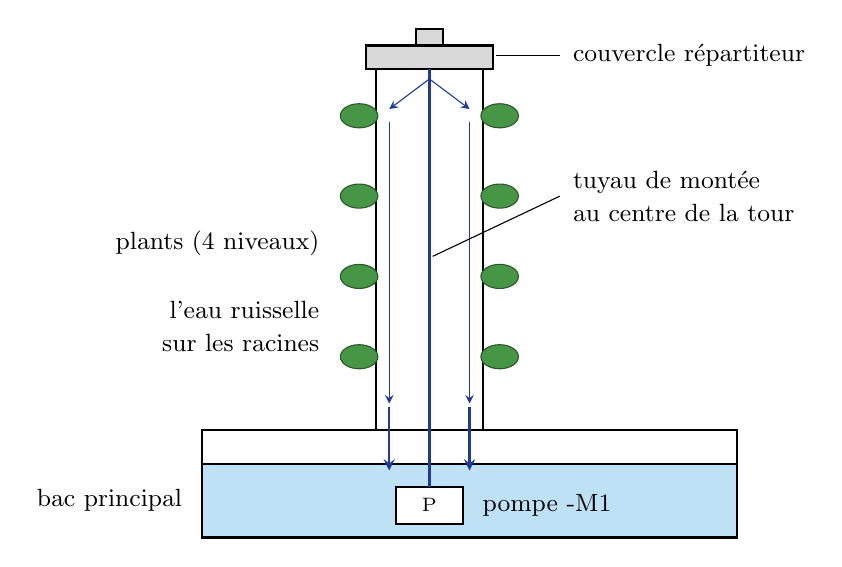
\begin{tikzpicture}[scale=0.85, >=stealth]
  \definecolor{eauc}{RGB}{190,225,245}
  \definecolor{plantec}{RGB}{70,150,70}
  \definecolor{bleuc}{RGB}{30,60,150}
  % bac
  \draw[thick, fill=eauc] (0,0) rectangle (8,1.1);
  \draw[thick] (0,1.1) rectangle (8,1.6);
  % tour (tube PVC)
  \draw[thick, fill=white] (2.6,1.6) rectangle (4.2,7.0);
  % couvercle
  \draw[thick, fill=gray!30] (2.45,7.0) rectangle (4.35,7.35);
  \draw[thick, fill=gray!30] (3.2,7.35) rectangle (3.6,7.6);
  % plants
  \foreach \y in {2.7,3.9,5.1,6.3} {
    \draw[fill=plantec, draw=plantec!60!black] (2.35,\y) ellipse (0.28 and 0.18);
    \draw[fill=plantec, draw=plantec!60!black] (4.45,\y) ellipse (0.28 and 0.18);
  }
  % pompe (sous la tour, dans le bac)
  \draw[thick, fill=white] (2.9,0.2) rectangle (3.9,0.75);
  \node at (3.4,0.48) {\scriptsize P};
  % tuyau de montee au centre de la tour
  \draw[very thick, bleuc] (3.4,0.75) -- (3.4,7.0);
  % eau projetee par le couvercle vers la paroi
  \draw[->, bleuc] (3.4,6.85) -- (2.8,6.4);
  \draw[->, bleuc] (3.4,6.85) -- (4.0,6.4);
  % ruissellement le long de la paroi
  \draw[->, bleuc] (2.8,6.2) -- (2.8,2.0);
  \draw[->, bleuc] (4.0,6.2) -- (4.0,2.0);
  % retour dans le bac
  \draw[->, thick, bleuc] (2.8,1.95) -- (2.8,1.0);
  \draw[->, thick, bleuc] (4.0,1.95) -- (4.0,1.0);
  % etiquettes
  \node[anchor=west] at (5.4,5.3) {\small tuyau de montée};
  \node[anchor=west] at (5.4,4.85) {\small au centre de la tour};
  \draw[thin] (5.35,5.1) -- (3.45,4.2);
  \node[anchor=west] at (5.4,7.2) {\small couvercle répartiteur};
  \draw[thin] (5.35,7.2) -- (4.4,7.2);
  \node[anchor=east] at (1.9,4.4) {\small plants (4 niveaux)};
  \node[anchor=east] at (1.9,3.4) {\small l'eau ruisselle};
  \node[anchor=east] at (1.9,2.9) {\small sur les racines};
  \node[anchor=east] at (-0.15,0.55) {\small bac principal};
  \node[anchor=west] at (4.05,0.48) {\small pompe -M1};
\end{tikzpicture}
\caption{Principe de la tour : la pompe, au fond du bac, envoie l'eau par un tuyau qui monte au centre de la tour jusqu'au couvercle. Le couvercle la répartit vers la paroi, elle ruisselle sur les racines puis retombe dans le bac. Schéma simplifié : les douze plants ne sont pas tous représentés.}
\end{figure}

\begin{aretenir}
Il n'existe pas de meilleur système dans l'absolu. Chacun convient à certaines plantes et à certaines contraintes. Choisir, c'est accepter ce que chaque système fait bien et ce qu'il fait moins bien.
\end{aretenir}

\subsection{Pourquoi une tour, et pourquoi de la laitue}

Dans la liste précédente, je n'ai pas choisi la tour : elle nous a été imposée par notre tuteur, qui nous la fournit, et ce au vu des délais. Il en va de même pour l'alimentation par énergie solaire. Cette année, nous sommes arrivés en troisième année de licence, et nous n'avons eu que trois mois, de septembre à novembre, pour mener le projet de bout en bout. Dans un délai aussi court, on ne peut pas comparer plusieurs systèmes, en construire un de chaque sorte et mesurer lequel marche le mieux. Il fallait partir d'un système précis, et c'est la tour qui a été retenue.

Je n'ai pas regretté ces contraintes. Avec si peu de temps, elles posent un cadre et donnent une direction à suivre : au lieu de me perdre à comparer toutes les possibilités, j'ai pu avancer tout de suite sur des choix précis. La tour a aussi de vrais atouts : peu de place au sol, une eau qui circule en circuit fermé, et un mécanisme assez simple à mesurer et à piloter. Elle impose aussi des contraintes, que les études de ce rapport détaillent : l'eau doit monter à environ un mètre, et la pompe doit tourner sans gaspiller la batterie.

Le même manque de temps a guidé le choix de la plante. Une culture longue dépasserait largement la durée du projet. La laitue, elle, est prête environ un mois après son repiquage, et elle supporte très bien l'hydroponie. Elle me permet de voir pousser quelque chose pendant le projet. Les valeurs de pH et de conductivité utilisées par la tour sont donc celles de la laitue, tout en gardant celles de la tomate cerise et du poivron en réserve dans le tableau de bord, pour une future culture.

\subsection{Ce que couvre ce rapport}

\textbf{Périmètre de ce rapport.} Ce rapport inclut uniquement le travail que j'ai effectué. Le projet se mène à deux, et la part de mon partenaire, \textbf{Gabriel Piritua}, consiste à monter l'armoire électrique et à construire le chariot qui transportera tout le système. Son travail n'est pas disponible pour l'instant : il n'apparaît donc pas dans ce rapport, et son coût n'est pas compté. Quand il sera disponible, il pourra s'ajouter à cet ensemble.

Mon travail, lui, va de la conception à la commande par ordinateur. Il comprend le calcul du circuit d'eau, le dimensionnement de l'alimentation solaire, la conception de la sonde de conductivité, la liste du matériel à acheter, le programme qui pilote la tour, le tableau de bord pour la surveiller, le suivi de la germination des laitues et enfin l'étude de ce que le système coûte et pourrait se vendre. Il comprend aussi un tutoriel pour que quelqu'un d'autre puisse l'installer.

Mon tuteur est Monsieur Anthony Utahia. Il m'accompagne tout au long du projet, et c'est avec lui que je valide chaque grande décision.

\Needspace{8\baselineskip}
\begin{aretenir}
Le projet est mené depuis septembre 2026. Il est en cours : certains éléments sont vérifiés sur la tour, d'autres sont calculés ou écrits mais pas encore essayés, et d'autres restent à construire. Ce rapport dit toujours dans quel état se trouve chaque élément.
\end{aretenir}

% ===== ETUDE HYDRAULIQUE =====
% =====================================================================
\partieENO{Le circuit d'eau}

Cette partie décrit comment l'eau circule dans la tour et ce que cela donne en chiffres. Je commence par le principe du circuit et par la difficulté qui a fait naître la pièce la plus particulière de la tour, le couvercle répartiteur. Je donne ensuite ses dimensions, puis je calcule le débit que la pompe fournit vraiment dans ce circuit. J'en déduis ce que reçoit chaque plant, la vitesse à laquelle le bac se renouvelle et la fréquence à laquelle il faut refaire le plein. Je compare ensuite les besoins en eau et en nutriments des plantes, au cours de leur vie, à la littérature, et je justifie pourquoi je n'ajoute pas de bac de secours. Je termine par le protocole de mesure, car aucune mesure n'est encore faite : tous les chiffres de cette partie sont théoriques.

\subsection{Le principe du circuit et la difficulté de départ}

La tour est un tube de PVC vertical de \qty{1}{m}, de diamètre intérieur \qty{144}{mm} et de diamètre extérieur \qty{159}{mm}. Il porte 12 plants de laitue. Une pompe immergée dans le bac de \qty{152}{L} envoie l'eau en haut de la tour par un tuyau flexible de \qty{9}{mm} de diamètre intérieur. L'eau y est répartie, elle ruisselle le long de la paroi, mouille les racines, puis retombe dans le bac par gravité. Le circuit est fermé : l'eau tourne en boucle et ne se perd que par la consommation des plantes et par l'évaporation. Le schéma hydraulique de la page suivante résume l'ensemble : bac, pompe, tour, dosage, sondes et appoint.

\schemapaysageC{Schema_hydraulique_hydroponie.pdf}{hydro}{Schéma hydraulique de la tour : bac unique, pompe de circulation -M1, pompes de dosage -M2 à -M4, sondes -B1 à -B4 et appoint manuel.}

Mon premier problème est la répartition. Si le tuyau débouche simplement en haut du tube, l'eau tombe en un jet central et suit le même chemin à chaque fois : les racines placées au bord ne sont presque pas mouillées, et celles du centre sont noyées. Il faut une pièce qui répartisse l'eau sur toute la circonférence du tube. J'ai donc conçu un couvercle répartiteur, imprimé en 3D, qui joue le rôle d'une pomme de douche.

\subsection{Le couvercle répartiteur}

Le couvercle se pose sur le haut du tube. Son embase s'emboîte dans le tube (diamètre \qty{144}{mm}, égal au diamètre intérieur du PVC) et sa bride de \qty{168}{mm} de diamètre recouvre la tranche du tube, qui fait \qty{159}{mm} à l'extérieur. L'eau arrive par un moyeu central de \qty{44}{mm}. Elle est ensuite guidée par \textbf{huit canaux} disposés en étoile, à \ang{45} les uns des autres, jusqu'à \textbf{huit trous de \qty{4}{mm} de diamètre} percés vers la paroi du tube. Chaque canal alimente un trou : l'eau sort donc en huit points régulièrement espacés et se répartit sur toute la circonférence.

Le plan du couvercle répartiteur, reproduit ci-dessous, donne ses dimensions et la position des huit canaux.

\begin{figure}[H]
\centering
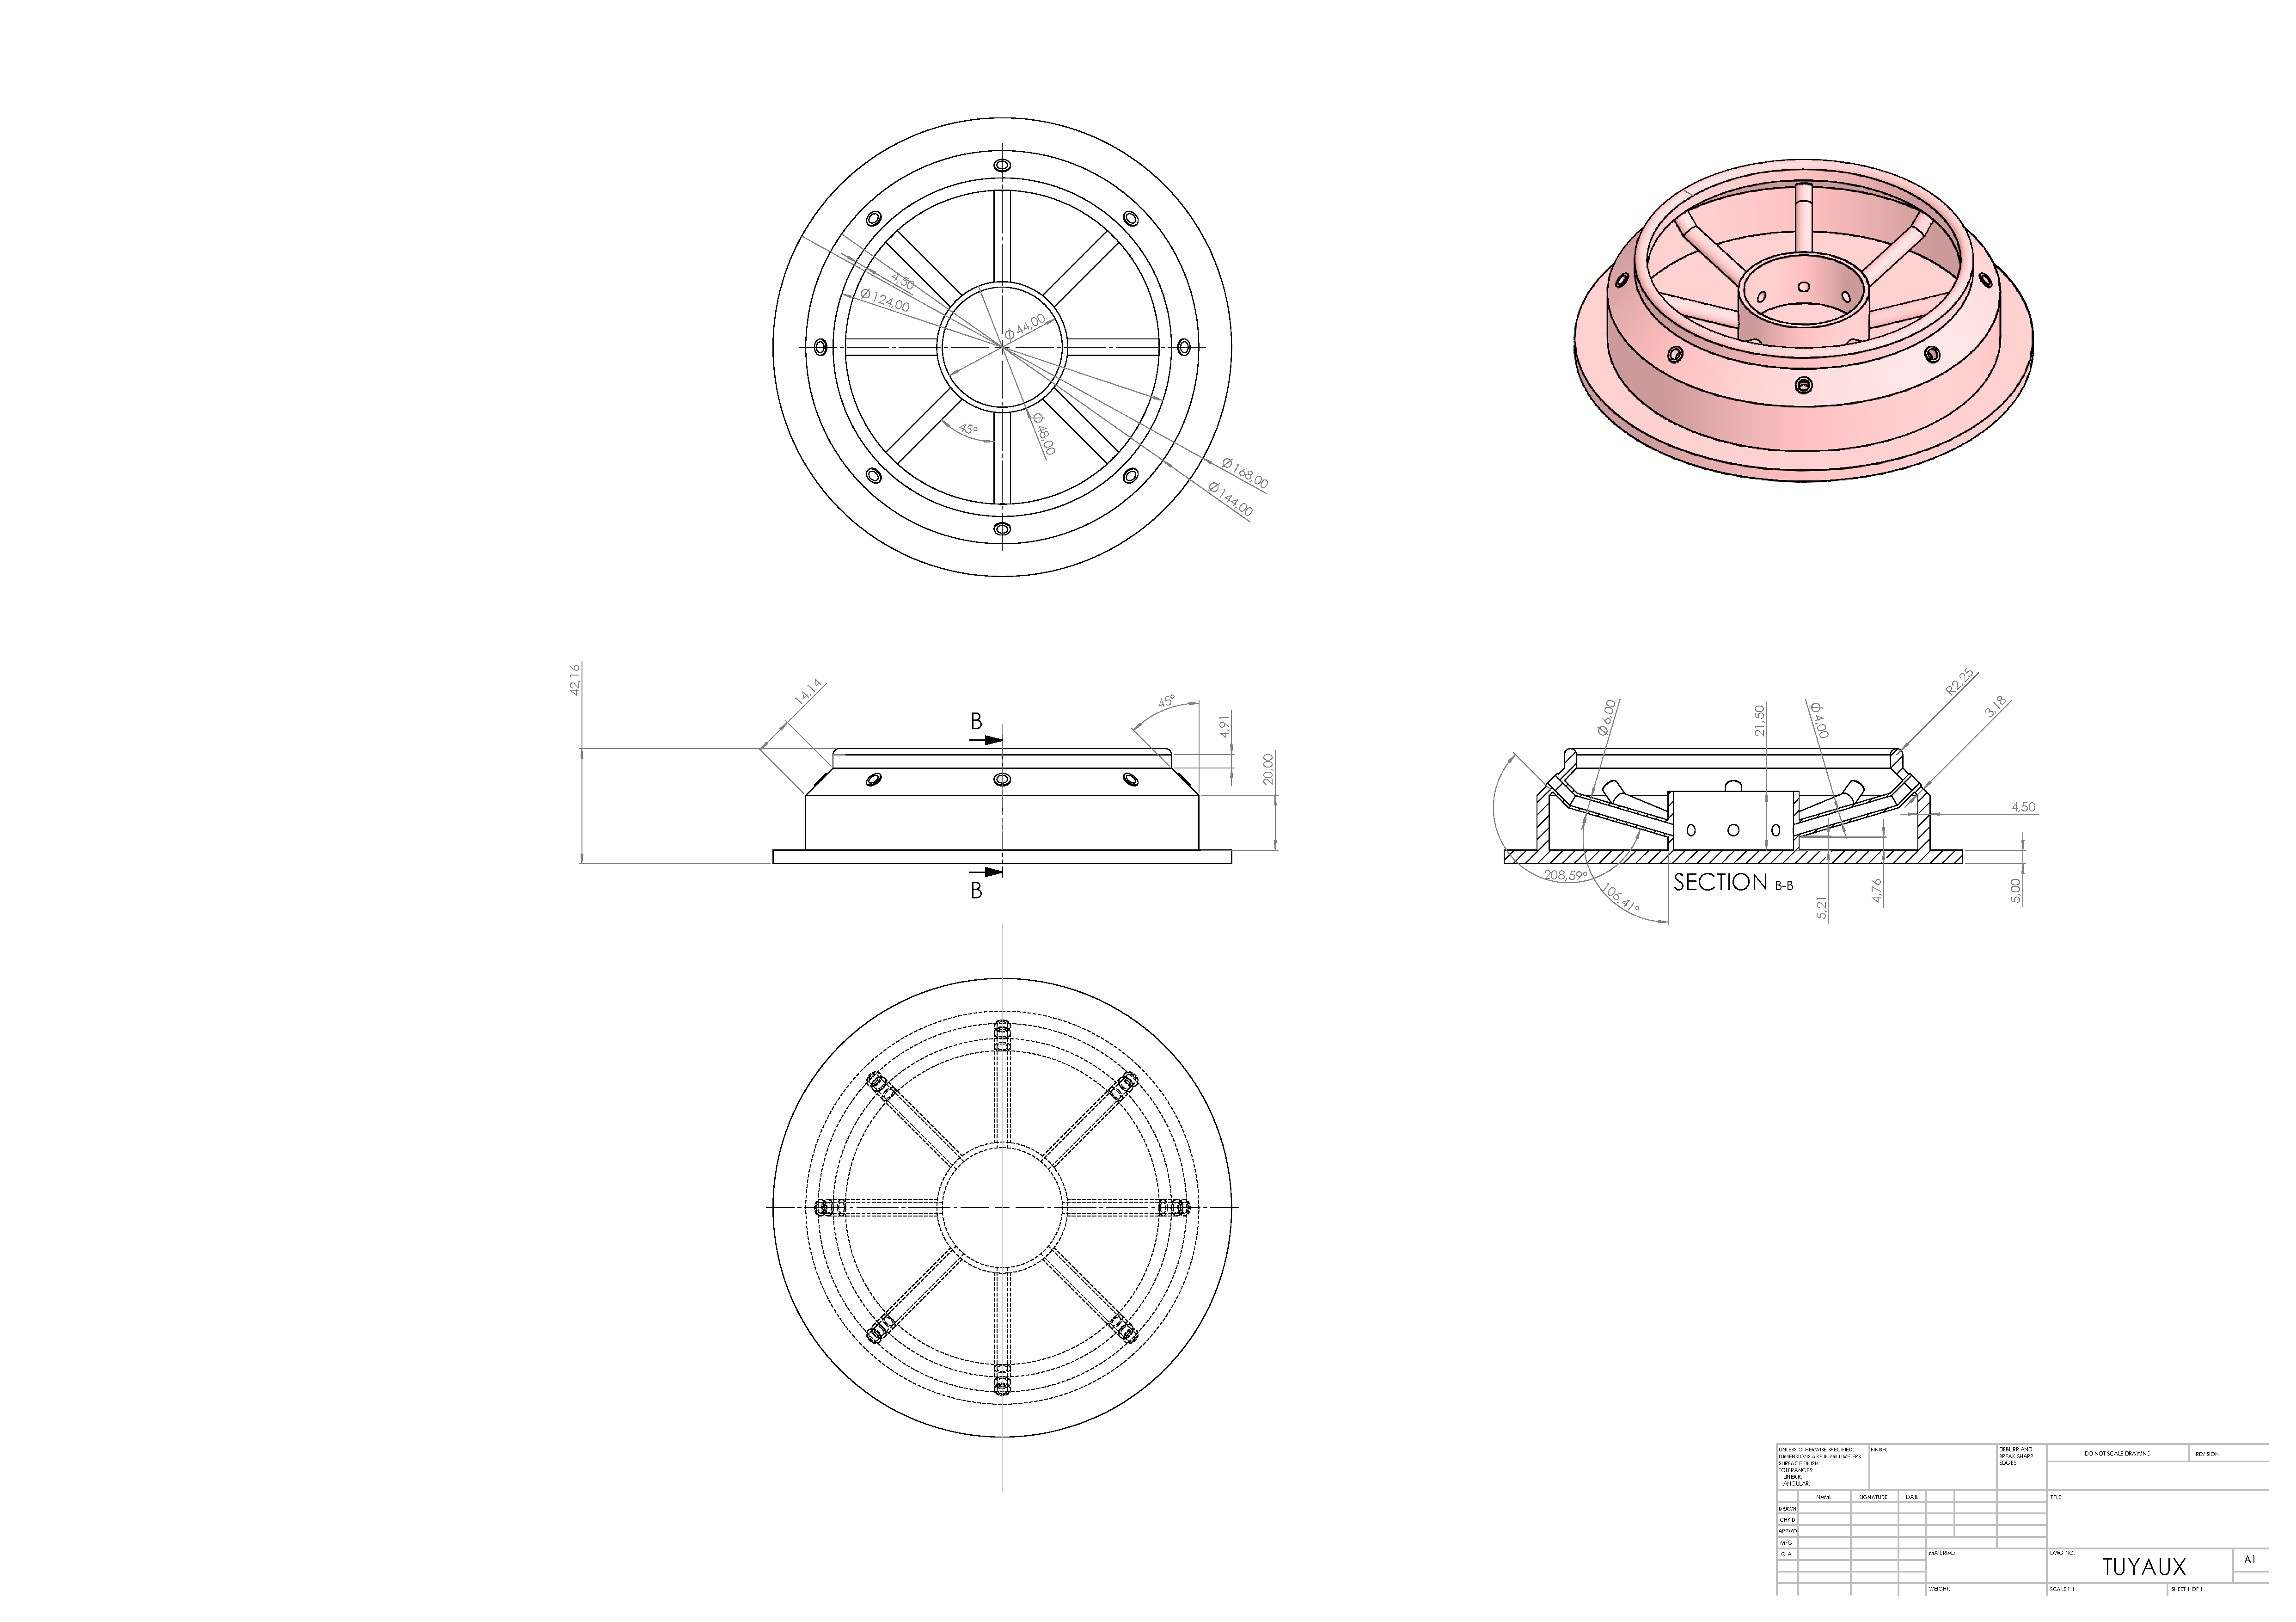
\includegraphics[page=1,trim=763bp 50bp 30bp 118bp,clip,width=0.86\textwidth]{Plan_couvercle_repartiteur.pdf}
\schemacap{planrep}{Plan du couvercle répartiteur : vue de dessus, vue de côté, vue de dessous avec les huit canaux et coupe B-B.}
\end{figure}

Le plan du couvercle répartiteur est la figure ci-dessus. Le plan de la pièce COUVERCLE (bouchon et embout) est reproduit en pleine page ci-dessous. Les deux plans complets sont aussi dans les annexes 1 et 2, à la fin du rapport.

\schemapaysageC[page=1]{Plan_couvercle_bouchon.pdf}{planbou}{Plan de la pièce COUVERCLE (bouchon et embout).}

Le choix du nombre de trous est un compromis. Plus il y en a, mieux l'eau est répartie, mais plus ils sont petits et plus ils risquent de se boucher avec les dépôts d'engrais. Huit trous de \qty{4}{mm} sont assez gros pour rester ouverts et assez nombreux pour que chaque trou arrose environ un huitième de la paroi, soit une zone d'environ \qty{57}{mm} de large sur le périmètre intérieur de \qty{452}{mm}.

\naturecalc{théorie, avec les dimensions mesurées sur la tour (bac, flexible, tube) et des valeurs de fiches techniques ; aucun débit ni aucune consommation n'est mesuré}
\begin{demonstration}[périmètre arrosé par chaque trou]
\resultat{p \approx \qty{57}{mm}}
Je note $D_t$ le diamètre intérieur du tube de la tour, en mètres (ici \qty{0,144}{m}), $P$ le périmètre intérieur du tube, en mètres, $n$ le nombre de trous (sans unité) et $p$ la longueur de paroi arrosée par un trou, en mètres. Le périmètre d'un cercle vaut $\pi$ fois son diamètre :
\begin{align*}
P &= \pi\, D_t\\
P &= \pi \times \qty{0,144}{m}\\
P &\approx \qty{0,452}{m}
\end{align*}
J'arrondis à trois chiffres. Les huit trous sont régulièrement espacés, donc chacun arrose la même longueur :
\begin{align*}
p &= \frac{P}{n}\\
p &= \frac{\qty{0,452}{m}}{8}\\
p &\approx \qty{0,0565}{m}
\end{align*}
soit environ \qty{57}{mm}, en arrondissant au millimètre.
\end{demonstration}

\subsection{Le point de fonctionnement de la pompe}

\subsubsection*{Ce que je cherche et ce que je suppose}

Je cherche le débit que la pompe fournit réellement dans ce circuit. La fiche de la pompe ne donne que deux points : à débit nul, elle monte l'eau à $H_{max} = \qty{5}{m}$ ; sans hauteur à vaincre, elle débite $Q_{max} = \qty{800}{L/h}$. Pour connaître le débit réel, je compare ce que la pompe peut fournir à ce que le circuit demande : le débit réel est celui pour lequel les deux hauteurs sont égales.

Faute de courbe constructeur, je relie les deux points connus par une droite. Je ne connais que ces deux points : je ne peux donc pas savoir de quel côté de la droite passe la vraie courbe de la pompe. Le débit de \qty{388}{L/h} est un résultat théorique, valable sous l'hypothèse de la droite, et non un débit garanti. Je le remplacerai par la mesure décrite dans le protocole, faite avec le circuit complet.

Les données du circuit sont les suivantes. Certaines sont mesurées, d'autres sont des hypothèses à vérifier.

\begin{table}[H]
\centering
\small
\renewcommand{\arraystretch}{1.1}
\begin{tabularx}{\textwidth}{|>{\raggedright\arraybackslash}p{5.6cm}|Y|>{\raggedright\arraybackslash}p{2.6cm}|}
\hline
\textbf{Donnée} & \textbf{Valeur retenue} & \textbf{Statut} \\
\hline
Volume du bac & \qty{152}{L} & mesuré \\
\hline
Pompe de circulation & \qty{800}{L/h} maximum, \qty{5}{m} maximum, \qty{12}{V}, \qty{19}{W} & fiche technique \\
\hline
Marche de la pompe & \qty{6,75}{h} par jour : le jour (10 h, de 7 h à 17 h), \qty{15}{min} de marche puis \qty{15}{min} d'arrêt, soit \qty{5}{h} ; la nuit (14 h, de 17 h à 7 h), 7 marches de \qty{15}{min} (17 h, 17 h 30, 21 h, 0 h, 3 h, 6 h et 6 h 30) $= \qty{1,75}{h}$ ; la coupure jour/nuit est choisie ici pour le bilan hydraulique, et la partie 5 la place à 6 h et 18 h, pour le même total & choix du projet \\
\hline
Diamètre intérieur du flexible & \qty{9}{mm} & mesuré \\
\hline
Longueur du flexible & \qty{1,8}{m} (\qty{0,4}{m} dans le bac, \qty{1,0}{m} le long de la tour, \qty{0,4}{m} de raccord) & hypothèse \\
\hline
Hauteur entre la surface du bac et le couvercle & \qty{1,2}{m} & hypothèse \\
\hline
Trous du couvercle & 8 trous de \qty{4}{mm} & plan \\
\hline
Pertes singulières & somme des coefficients $K = 2,8$ & hypothèse \\
\hline
Contraction du jet à la sortie d'un trou & coefficient $C_d = 0,62$ & hypothèse \\
\hline
Eau à \qty{25}{\celsius} & masse volumique \qty{997}{kg/m^3}, viscosité cinématique \qty{0,893e-6}{m^2/s} & tables \\
\hline
\end{tabularx}
\caption{Données du circuit d'eau.}
\end{table}

Les pertes singulières regroupent l'entrée dans la pompe et le raccord (coefficient \num{0,5}), deux coudes à \ang{90} (\num{0,9} chacun) et l'entrée dans le couvercle (\num{0,5}), soit $K = 0,5 + 2 \times 0,9 + 0,5 = 2,8$.

\subsubsection*{La courbe de la pompe}

\naturecalc{théorie, avec les dimensions mesurées sur la tour (bac, flexible, tube) et des valeurs de fiches techniques ; aucun débit ni aucune consommation n'est mesuré}
\begin{demonstration}[courbe linéaire de la pompe]
\resultat{H_p(Q) = H_{max}\left(1 - \dfrac{Q}{Q_{max}}\right)}
Je note $Q$ le débit de la pompe, en litres par heure, et $H_p$ la hauteur d'eau qu'elle peut fournir à ce débit, en mètres. Je cherche une droite de la forme :
\begin{align*}
H_p(Q) &= \alpha\,Q + \beta
\end{align*}
où $\alpha$ est sa pente, en mètres par litre par heure, et $\beta$ son ordonnée à l'origine, en mètres. Elle passe par le point $(Q = 0\,;\,H_p = H_{max})$. En remplaçant $Q$ par $0$ :
\begin{align*}
H_p(0) &= \alpha \times 0 + \beta\\
H_{max} &= \beta
\end{align*}
Elle passe aussi par le point $(Q = Q_{max}\,;\,H_p = 0)$. En remplaçant :
\begin{align*}
0 &= \alpha\, Q_{max} + H_{max}\\
\alpha\, Q_{max} &= -H_{max}\\
\alpha &= -\frac{H_{max}}{Q_{max}}
\end{align*}
En remettant $\alpha$ et $\beta$ dans l'équation de la droite :
\begin{align*}
H_p(Q) &= -\frac{H_{max}}{Q_{max}}\,Q + H_{max}\\
H_p(Q) &= H_{max}\left(1 - \frac{Q}{Q_{max}}\right)
\end{align*}
Avec les valeurs de la fiche :
\begin{align*}
H_p(Q) &= \qty{5}{m}\times\left(1 - \frac{Q}{\qty{800}{L/h}}\right)
\end{align*}
\end{demonstration}

\subsubsection*{La courbe du circuit}

La courbe du circuit donne la hauteur que la pompe doit fournir pour faire passer un débit donné dans le tuyau et dans le couvercle. Je pars de la conservation de l'énergie de l'eau, puis j'ajoute les pertes.

\naturecalc{théorie, avec les dimensions mesurées sur la tour (bac, flexible, tube) et des valeurs de fiches techniques ; aucun débit ni aucune consommation n'est mesuré}
\begin{demonstration}[hauteur demandée par le circuit]
\resultat{H_r = H_g + \dfrac{v_j^2}{2g} + h_r + h_s}
Je considère une tranche d'eau de masse $m$, en kilogrammes, de volume $m/\rho$, avec $\rho$ la masse volumique de l'eau, en kilogrammes par mètre cube. Elle a trois énergies :
\begin{align*}
E_{pression} &= p\,\frac{m}{\rho}\\
E_{cin} &= \frac{1}{2}\,m\,v^2\\
E_{pot} &= m\,g\,z
\end{align*}
où $p$ est la pression, en pascals, $v$ la vitesse, en mètres par seconde, $g = \qty{9,81}{m/s^2}$ l'accélération de la pesanteur et $z$ l'altitude, en mètres. Je divise chaque énergie par le poids $m g$ de la tranche, en newtons : j'obtiens une énergie par unité de poids, qui s'exprime en mètres, donc une hauteur :
\begin{align*}
e &= \frac{p}{\rho g} + \frac{v^2}{2g} + z
\end{align*}
Entre la surface du bac (point 1) et la sortie des trous du couvercle (point 2), la pompe apporte la hauteur $H$, en mètres, et les frottements en retirent $\Delta H$, en mètres :
\begin{align*}
\frac{p_1}{\rho g} + \frac{v_1^2}{2g} + z_1 + H &= \frac{p_2}{\rho g} + \frac{v_2^2}{2g} + z_2 + \Delta H
\end{align*}
Au point 1, l'eau est à la pression atmosphérique $p_{atm}$ et presque immobile, car la surface du bac est très grande devant le tuyau : $p_1 = p_{atm}$ et $v_1 \approx 0$. Au point 2, l'eau sort à l'air libre : $p_2 = p_{atm}$, avec la vitesse de jet $v_j$. Les pressions atmosphériques s'annulent. En notant $H_g = z_2 - z_1$ la hauteur entre la surface du bac et le couvercle, en mètres :
\begin{align*}
H &= H_g + \frac{v_j^2}{2g} + \Delta H
\end{align*}
Les pertes se séparent en pertes régulières $h_r$ (frottement le long du tuyau) et pertes singulières $h_s$ (coudes, raccords), toutes en mètres :
\begin{align*}
\Delta H &= h_r + h_s
\end{align*}
La hauteur $H$ que la pompe doit fournir est la hauteur demandée par le circuit, notée $H_r$ :
\begin{align*}
H_r &= H_g + \frac{v_j^2}{2g} + h_r + h_s
\end{align*}
\end{demonstration}

\naturecalc{théorie, avec les dimensions mesurées sur la tour (bac, flexible, tube) et des valeurs de fiches techniques ; aucun débit ni aucune consommation n'est mesuré}
\begin{demonstration}[perte de charge régulière]
\resultat{h_r = \lambda\,\dfrac{L}{D}\,\dfrac{v^2}{2g}}
Je note $L$ la longueur du tuyau, en mètres, $D$ son diamètre intérieur, en mètres, et $v$ la vitesse moyenne de l'eau, en mètres par seconde. J'isole un tronçon de tuyau où l'écoulement est établi : la vitesse ne change pas, donc la quantité de mouvement de l'eau ne change pas et les forces se compensent. La différence de pression $\Delta p$, en pascals, sur les deux sections pousse l'eau ; la contrainte de frottement $\tau_p$, en pascals, sur la paroi la retient :
\begin{align*}
\Delta p \cdot \frac{\pi D^2}{4} &= \tau_p \cdot \pi D L
\end{align*}
Je divise les deux membres par $\pi D^2/4$ :
\begin{align*}
\Delta p &= \frac{4\,\tau_p\,L}{D}
\end{align*}
La contrainte $\tau_p$ dépend de $\rho$, de $v$ et de la viscosité. La seule grandeur homogène à une pression que l'on peut former avec $\rho$ et $v$ est $\rho v^2$. Le rapport $\tau_p/(\rho v^2)$ est donc un nombre sans dimension : il ne peut dépendre que du nombre de Reynolds $Re = vD/\nu$, avec $\nu$ la viscosité cinématique de l'eau, en mètres carrés par seconde. Je l'écris par convention $\lambda/8$, où $\lambda$ est le coefficient de frottement, sans unité :
\begin{align*}
\tau_p &= \frac{\lambda}{8}\,\rho v^2
\end{align*}
En remplaçant dans l'expression de $\Delta p$ :
\begin{align*}
\Delta p &= \frac{4 L}{D}\times\frac{\lambda}{8}\,\rho v^2\\
\Delta p &= \lambda\,\frac{L}{D}\,\frac{\rho v^2}{2}
\end{align*}
Pour l'exprimer en hauteur d'eau, je divise par $\rho g$ :
\begin{align*}
h_r &= \frac{\Delta p}{\rho g}\\
h_r &= \lambda\,\frac{L}{D}\,\frac{v^2}{2g}
\end{align*}
Pour un tuyau lisse en régime turbulent ($4000 < Re < 10^5$), la loi expérimentale que j'utilise pour $\lambda$ est :
\begin{align*}
\lambda &= 0,316\,Re^{-1/4}
\end{align*}
\end{demonstration}

\naturecalc{théorie, avec les dimensions mesurées sur la tour (bac, flexible, tube) et des valeurs de fiches techniques ; aucun débit ni aucune consommation n'est mesuré}
\begin{demonstration}[perte singulière, vitesse du tuyau et vitesse du jet]
\resultat{H_r(Q) = H_g + \left(\lambda\dfrac{L}{D} + K\right)\dfrac{Q^2}{2gA^2} + \dfrac{Q^2}{2g\,a^2}}
Chaque coude ou raccord dissipe une fraction de l'énergie cinétique de l'eau, proportionnelle à $v^2/(2g)$ par un coefficient $K_i$ propre à la pièce, sans unité. En additionnant toutes les pièces :
\begin{align*}
h_s &= \left(\sum K_i\right)\frac{v^2}{2g}\\
h_s &= K\,\frac{v^2}{2g}
\end{align*}
Le débit volumique $Q$, en mètres cubes par seconde, est le même dans toute section du tuyau. Avec $A$ la section intérieure du tuyau, en mètres carrés :
\begin{align*}
Q &= v\,A\\
v &= \frac{Q}{A}\\
A &= \frac{\pi D^2}{4}
\end{align*}
À la sortie de chaque trou de diamètre $d$, en mètres, le jet se contracte à la section $C_d\,\pi d^2/4$. Avec $n$ trous, la section utile totale $a$, en mètres carrés, vaut :
\begin{align*}
a &= n\,C_d\,\frac{\pi d^2}{4}
\end{align*}
et la vitesse du jet $v_j$, en mètres par seconde, vaut :
\begin{align*}
v_j &= \frac{Q}{a}
\end{align*}
Je remplace $h_r$, $h_s$, $v$ et $v_j$ dans $H_r$ :
\begin{align*}
H_r(Q) &= H_g + \left(\lambda\frac{L}{D} + K\right)\frac{v^2}{2g} + \frac{v_j^2}{2g}\\
H_r(Q) &= H_g + \left(\lambda\frac{L}{D} + K\right)\frac{Q^2}{2gA^2} + \frac{Q^2}{2g\,a^2}
\end{align*}
\end{demonstration}

\naturecalc{théorie, avec les dimensions mesurées sur la tour (bac, flexible, tube) et des valeurs de fiches techniques ; aucun débit ni aucune consommation n'est mesuré}
\begin{demonstration}[sections du tuyau et du couvercle]
\resultat{a \approx \qty{62,3}{mm^2}\ \text{pour}\ A \approx \qty{63,6}{mm^2}}
La section intérieure du flexible, de diamètre $D = \qty{9}{mm} = \qty{0,009}{m}$, vaut :
\begin{align*}
A &= \frac{\pi D^2}{4}\\
A &= \frac{\pi \times (\qty{0,009}{m})^2}{4}\\
A &\approx \qty{6,36e-5}{m^2}
\end{align*}
La section utile des huit trous de diamètre $d = \qty{4}{mm} = \qty{0,004}{m}$, avec $C_d = 0,62$, vaut :
\begin{align*}
a &= n\,C_d\,\frac{\pi d^2}{4}\\
a &= 8 \times 0,62 \times \frac{\pi \times (\qty{0,004}{m})^2}{4}\\
a &\approx \qty{6,23e-5}{m^2}
\end{align*}
Les deux sections sont presque égales (rapport $A/a \approx 1,02$) : le couvercle ne freine presque pas l'eau, il la répartit sans former un jet rapide.
\end{demonstration}

\subsubsection*{Le point de fonctionnement}

Le débit réel est celui pour lequel la hauteur fournie par la pompe égale la hauteur demandée par le circuit : $H_p(Q) = H_r(Q)$. Comme le coefficient $\lambda$ dépend lui-même du débit, je ne peux pas isoler $Q$ à la main : je résous l'équation numériquement avec un script. Je vérifie ensuite le résultat terme par terme.

La figure suivante superpose la courbe de la pompe et celle du circuit : leur croisement est le point de fonctionnement.

\begin{figure}[H]
\centering
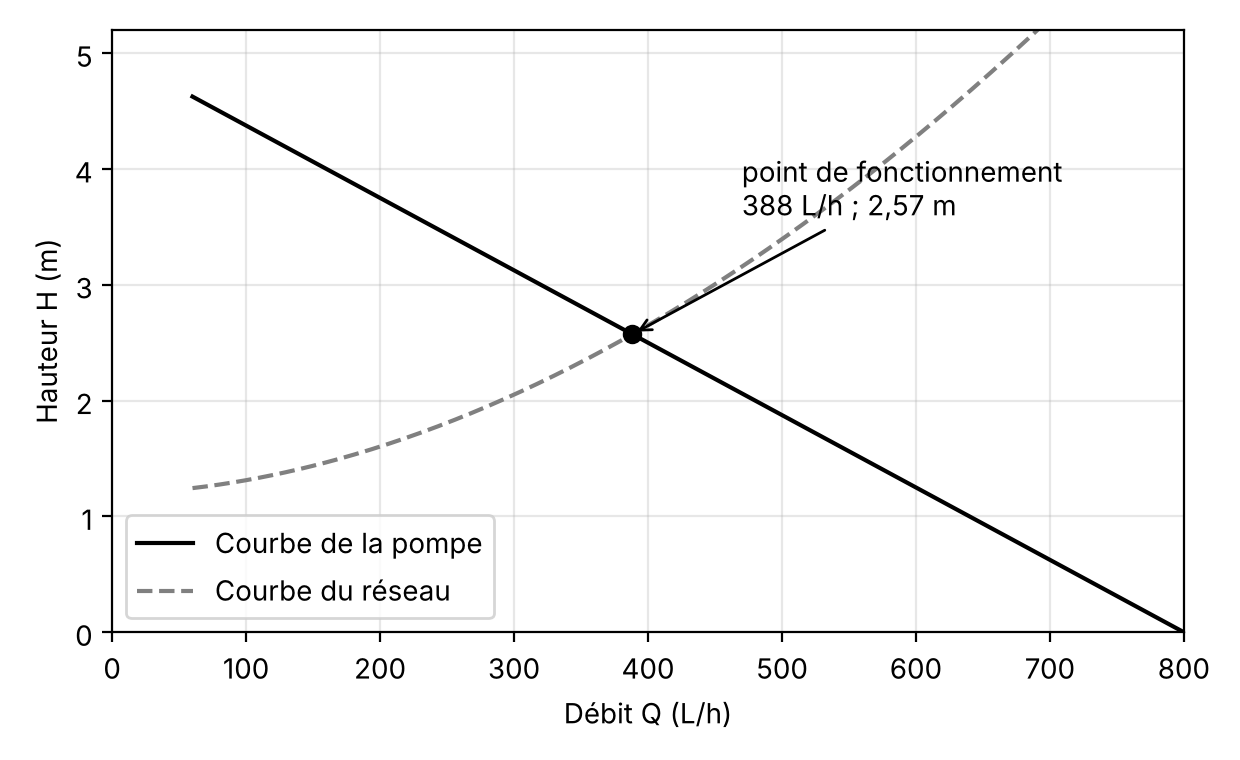
\includegraphics[width=0.82\textwidth]{img/point_fonct.png}
\caption{Courbe de la pompe, courbe du circuit et point de fonctionnement.}
\end{figure}

\naturecalc{théorie, avec les dimensions mesurées sur la tour (bac, flexible, tube) et des valeurs de fiches techniques ; aucun débit ni aucune consommation n'est mesuré}
\begin{demonstration}[vérification du point de fonctionnement]
\resultat{Q \approx \qty{388}{L/h}\ \text{sous}\ H \approx \qty{2,57}{m}}
Le script donne le débit $Q = \qty{1,0787e-4}{m^3/s}$. Je le convertis en litres par heure, sachant qu'un mètre cube vaut \qty{1000}{L} et qu'une heure vaut \qty{3600}{s} :
\begin{align*}
Q &= \qty{1,0787e-4}{m^3/s} \times \qty{1000}{L/m^3} \times \qty{3600}{s/h}\\
Q &\approx \qty{388,3}{L/h}
\end{align*}
La vitesse dans le tuyau vaut :
\begin{align*}
v &= \frac{Q}{A}\\
v &= \frac{\qty{1,0787e-4}{m^3/s}}{\qty{6,362e-5}{m^2}}\\
v &\approx \qty{1,696}{m/s}
\end{align*}
Le nombre de Reynolds vaut :
\begin{align*}
Re &= \frac{v\,D}{\nu}\\
Re &= \frac{\qty{1,696}{m/s}\times\qty{0,009}{m}}{\qty{0,893e-6}{m^2/s}}\\
Re &\approx 17\,100
\end{align*}
Ce nombre est supérieur à $4000$ : l'écoulement est turbulent et la loi de $\lambda$ s'applique.
\begin{align*}
\lambda &= 0,316 \times 17\,089^{-1/4}\\
\lambda &= \frac{0,316}{11,43}\\
\lambda &\approx 0,0276
\end{align*}
L'énergie cinétique par unité de poids dans le tuyau vaut :
\begin{align*}
\frac{v^2}{2g} &= \frac{(\qty{1,696}{m/s})^2}{2\times\qty{9,81}{m/s^2}}\\
\frac{v^2}{2g} &\approx \qty{0,1465}{m}
\end{align*}
Le rapport $L/D$ vaut $\qty{1,8}{m}/\qty{0,009}{m} = 200$. Les pertes régulières valent :
\begin{align*}
h_r &= 0,0276 \times 200 \times \qty{0,1465}{m}\\
h_r &\approx \qty{0,810}{m}
\end{align*}
Les pertes singulières valent :
\begin{align*}
h_s &= 2,8 \times \qty{0,1465}{m}\\
h_s &\approx \qty{0,410}{m}
\end{align*}
La vitesse du jet vaut :
\begin{align*}
v_j &= \frac{Q}{a}\\
v_j &= \frac{\qty{1,0787e-4}{m^3/s}}{\qty{6,233e-5}{m^2}}\\
v_j &\approx \qty{1,731}{m/s}
\end{align*}
et son énergie cinétique par unité de poids :
\begin{align*}
\frac{v_j^2}{2g} &= \frac{(\qty{1,731}{m/s})^2}{2\times\qty{9,81}{m/s^2}}\\
\frac{v_j^2}{2g} &\approx \qty{0,153}{m}
\end{align*}
La hauteur demandée par le circuit vaut :
\begin{align*}
H_r &= \qty{1,2}{m} + \qty{0,810}{m} + \qty{0,410}{m} + \qty{0,153}{m}\\
H_r &\approx \qty{2,573}{m}
\end{align*}
La hauteur fournie par la pompe vaut :
\begin{align*}
H_p &= \qty{5}{m}\times\left(1 - \frac{\qty{388,3}{L/h}}{\qty{800}{L/h}}\right)\\
H_p &= \qty{5}{m}\times 0,5146\\
H_p &\approx \qty{2,573}{m}
\end{align*}
Les deux hauteurs sont égales : le point de fonctionnement est vérifié. Les pertes dans le flexible ($h_r + h_s$, soit \qty{1,22}{m}) pèsent presque autant que la montée elle-même (\qty{1,2}{m}) : c'est le flexible fin de \qty{9}{mm} qui limite le débit, et non le couvercle.
\end{demonstration}

\naturecalc{théorie, avec les dimensions mesurées sur la tour (bac, flexible, tube) et des valeurs de fiches techniques ; aucun débit ni aucune consommation n'est mesuré}
\begin{demonstration}[pression avant le couvercle et hauteur du jet]
\resultat{p - p_{atm} \approx \qty{60}{Pa}\ \text{et}\ h_{jet} \approx \qty{15}{cm}}
Entre le tuyau juste avant le couvercle (vitesse $v$, pression $p$) et le jet (vitesse $v_j$, pression atmosphérique), à la même altitude et sans perte (déjà comptée par $C_d$), la conservation de l'énergie donne :
\begin{align*}
\frac{p - p_{atm}}{\rho g} + \frac{v^2}{2g} &= \frac{v_j^2}{2g}
\end{align*}
Je multiplie par $\rho g$ et j'isole la surpression, en pascals :
\begin{align*}
p - p_{atm} &= \frac{\rho}{2}\left(v_j^2 - v^2\right)\\
p - p_{atm} &= \frac{\qty{997}{kg/m^3}}{2}\times\left((\qty{1,731}{m/s})^2 - (\qty{1,696}{m/s})^2\right)\\
p - p_{atm} &\approx \qty{60}{Pa}
\end{align*}
soit environ $\qty{0,0006}{bar}$ : l'eau arrive presque sans pression au couvercle.

Si un trou était dirigé vers le haut, son jet monterait, sans frottement de l'air, jusqu'à ce que toute son énergie cinétique soit devenue potentielle :
\begin{align*}
\frac{1}{2}\,m\,v_j^2 &= m\,g\,h_{jet}\\
h_{jet} &= \frac{v_j^2}{2g}\\
h_{jet} &\approx \qty{0,153}{m}
\end{align*}
soit environ \qty{15}{cm}. Cette hauteur se mesure facilement et permet de vérifier le débit (protocole en fin de partie).
\end{demonstration}

\naturecalc{théorie, avec les dimensions mesurées sur la tour (bac, flexible, tube) et des valeurs de fiches techniques ; aucun débit ni aucune consommation n'est mesuré}
\begin{demonstration}[puissance hydraulique et rendement]
\resultat{P_h \approx \qty{2,7}{W}\ \text{et}\ \eta \approx 0,14}
La pompe élève chaque seconde un volume $Q$, c'est-à-dire un poids $\rho g Q$, en newtons par seconde, d'une hauteur $H$. Sa puissance hydraulique $P_h$, en watts, vaut donc :
\begin{align*}
P_h &= \rho\,g\,Q\,H\\
P_h &= \qty{997}{kg/m^3}\times\qty{9,81}{m/s^2}\times\qty{1,0787e-4}{m^3/s}\times\qty{2,573}{m}\\
P_h &\approx \qty{2,71}{W}
\end{align*}
Comparée aux $P_e = \qty{19}{W}$ électriques de la pompe, le rendement global $\eta$ (sans unité) vaut :
\begin{align*}
\eta &= \frac{P_h}{P_e}\\
\eta &= \frac{\qty{2,71}{W}}{\qty{19}{W}}\\
\eta &\approx 0,14
\end{align*}
Ce rendement faible est normal pour une petite pompe utilisée loin de son point de meilleur rendement. Il ne change pas la consommation électrique retenue dans l'étude énergétique, \qty{19}{W}.
\end{demonstration}

\subsubsection*{Sensibilité au diamètre du flexible}

Le diamètre du flexible est la donnée qui pèse le plus. Le tableau donne le point de fonctionnement pour d'autres flexibles courants, avec le même couvercle et la même longueur.

\begin{table}[H]
\centering
\small
\renewcommand{\arraystretch}{1.1}
\begin{tabularx}{\textwidth}{|Y|Y|Y|Y|}
\hline
\textbf{Diamètre intérieur (mm)} & \textbf{Débit (L/h)} & \textbf{Vitesse (m/s)} & \textbf{Hauteur (m)} \\
\hline
\textbf{9 (mon flexible)} & \textbf{388} & \textbf{1,70} & \textbf{2,57} \\
\hline
10 & 431 & 1,52 & 2,31 \\
\hline
13 & 505 & 1,06 & 1,84 \\
\hline
16 & 535 & 0,74 & 1,66 \\
\hline
\end{tabularx}
\caption{Point de fonctionnement selon le diamètre du flexible.}
\end{table}

Un flexible plus gros augmenterait le débit d'environ 30 \% (de \qty{388}{L/h} à \qty{505}{L/h} pour \qty{13}{mm}). Ce n'est pas nécessaire : on verra que \qty{388}{L/h} suffisent largement.

\subsection{Débit par plant et renouvellement du bac}

\naturecalc{théorie, avec les dimensions mesurées sur la tour (bac, flexible, tube) et des valeurs de fiches techniques ; aucun débit ni aucune consommation n'est mesuré}
\begin{demonstration}[débit par plant]
\resultat{q_{plant} \approx \qty{32}{L/h}}
Je note $n_p = 12$ le nombre de plants. Le couvercle répartit le débit $Q$ sur toute la paroi, donc chaque plant reçoit en moyenne :
\begin{align*}
q_{plant} &= \frac{Q}{n_p}\\
q_{plant} &= \frac{\qty{388,3}{L/h}}{12}\\
q_{plant} &\approx \qty{32,4}{L/h}
\end{align*}
soit \qty{0,54}{L/min}. Pour une tour à ruissellement, je retiens un besoin minimal de \qty{2}{L/h} par godet pendant la marche, pour que la paroi et les racines restent mouillées sur toute la hauteur. Le débit disponible est donc environ 16 fois supérieur à ce besoin :
\begin{align*}
\frac{q_{plant}}{q_{min}} &= \frac{\qty{32,4}{L/h}}{\qty{2}{L/h}}\\
\frac{q_{plant}}{q_{min}} &\approx 16
\end{align*}
\end{demonstration}

Cette division suppose une répartition égale, ce que le couvercle ne garantit pas : il n'a que 8 sorties pour 12 emplacements. Le débit moyen par sortie vaut $q_{trou} = \qty{388,3}{L/h} / 8 \approx \qty{48,5}{L/h}$. L'eau ruisselle ensuite le long de la paroi et peut mouiller plusieurs godets, mais je ne peux pas annoncer un débit réel par plant tant que la répartition n'est pas mesurée. Je retiens donc le débit moyen de \qty{32}{L/h} par plant comme un ordre de grandeur, et le vrai critère reste visuel : les huit zones arrosées doivent se rejoindre et toutes les racines doivent être mouillées pendant la marche. Ce sera vérifié à l'essai.

\naturecalc{théorie, avec les dimensions mesurées sur la tour (bac, flexible, tube) et des valeurs de fiches techniques ; aucun débit ni aucune consommation n'est mesuré}
\begin{demonstration}[temps de renouvellement du bac]
\resultat{\tau \approx \qty{23,5}{min}}
Le temps de renouvellement $\tau$ est la durée pour que la pompe fasse passer dans la tour un volume égal à celui du bac $V = \qty{152}{L}$ :
\begin{align*}
\tau &= \frac{V}{Q}\\
\tau &= \frac{\qty{152}{L}}{\qty{388,3}{L/h}}\\
\tau &\approx \qty{0,391}{h}
\end{align*}
Je multiplie par \qty{60}{min/h} :
\begin{align*}
\tau &= \qty{0,391}{h}\times\qty{60}{min/h}\\
\tau &\approx \qty{23,5}{min}
\end{align*}
Pendant les $t_{marche} = \qty{6,75}{h}$ de marche par jour, le volume du bac passe dans la tour :
\begin{align*}
N_j &= \frac{Q\,t_{marche}}{V}\\
N_j &= \frac{\qty{388,3}{L/h}\times\qty{6,75}{h/j}}{\qty{152}{L}}\\
N_j &= \frac{\qty{2621}{L/j}}{\qty{152}{L}}\\
N_j &\approx 17{,}2\ \text{fois par jour}
\end{align*}
Une période de marche de \qty{15}{min} fait donc passer environ $\qty{15}{min}/\qty{23,5}{min} \approx 64\ \%$ du volume du bac dans la tour.
\end{demonstration}

\subsection{Consommation d'eau et fréquence de l'appoint}

L'eau quitte le bac de deux façons : elle est absorbée par les plants (transpirée par les feuilles) et elle s'évapore au contact de l'air. Les chiffres suivants sont des hypothèses de départ, à remplacer par les mesures.

\begin{table}[H]
\centering
\small
\renewcommand{\arraystretch}{1.1}
\begin{tabularx}{\textwidth}{|>{\raggedright\arraybackslash}p{5.2cm}|Y|}
\hline
\textbf{Hypothèse} & \textbf{Valeur retenue} \\
\hline
Consommation d'une laitue adulte (pointe) & \qty{0,30}{L/j} par plant, pendant les 10 derniers jours avant la récolte \\
\hline
Consommation moyenne sur le cycle & \qty{0,15}{L/j} par plant : une laitue a peu de feuilles la première moitié du cycle, puis consomme de plus en plus, d'où une moyenne d'environ la moitié de la pointe \\
\hline
Évaporation & surface d'eau libre de \qty{0,10}{m^2} (ouvertures, godets, parois mouillées) et \qty{5}{mm/j}, eau tiède et air chaud et humide \\
\hline
Bac plein & bac de \qty{0,70}{m} sur \qty{0,45}{m}, soit une surface $S_{bac} = \qty{0,70}{m}\times\qty{0,45}{m} \approx \qty{0,315}{m^2}$, rempli avec \qty{152}{L} (hauteur d'eau $\qty{0,152}{m^3}/\qty{0,315}{m^2} \approx \qty{0,48}{m}$, bac plein) \\
\hline
Appoint toléré & baisse de 10 \% du volume du bac \\
\hline
\end{tabularx}
\caption{Hypothèses du bilan hydrique.}
\end{table}

\naturecalc{théorie, avec les dimensions mesurées sur la tour (bac, flexible, tube) et des valeurs de fiches techniques ; aucun débit ni aucune consommation n'est mesuré}
\begin{demonstration}[évaporation et consommation journalière]
\resultat{C_{pic} = \qty{4,1}{L/j}\ \text{et}\ C_{moy} = \qty{2,3}{L/j}}
Une lame d'eau de \qty{1}{mm} d'épaisseur sur \qty{1}{m^2} représente un volume de :
\begin{align*}
\qty{e-3}{m}\times\qty{1}{m^2} &= \qty{e-3}{m^3}\\
&= \qty{1}{L}
\end{align*}
Je note $S_e = \qty{0,10}{m^2}$ la surface d'eau libre et $e = \qty{5}{mm/j}$ la hauteur évaporée par jour. L'évaporation $E$, en litres par jour, vaut :
\begin{align*}
E &= S_e \times e \times \qty{1}{L/(mm\cdot m^2)}\\
E &= \qty{0,10}{m^2}\times\qty{5}{mm/j}\times\qty{1}{L/(mm\cdot m^2)}\\
E &= \qty{0,5}{L/j}
\end{align*}
La consommation journalière $C$ du bac, en litres par jour, est la somme de ce que boivent les $n_p$ plants (chacun $c$, en litres par jour) et de l'évaporation :
\begin{align*}
C &= n_p\,c + E
\end{align*}
En pointe ($c = \qty{0,30}{L/j}$) :
\begin{align*}
C_{pic} &= 12\times\qty{0,30}{L/j} + \qty{0,5}{L/j}\\
C_{pic} &= \qty{3,6}{L/j} + \qty{0,5}{L/j}\\
C_{pic} &= \qty{4,1}{L/j}
\end{align*}
En moyenne sur le cycle ($c = \qty{0,15}{L/j}$) :
\begin{align*}
C_{moy} &= 12\times\qty{0,15}{L/j} + \qty{0,5}{L/j}\\
C_{moy} &= \qty{1,8}{L/j} + \qty{0,5}{L/j}\\
C_{moy} &= \qty{2,3}{L/j}
\end{align*}
\end{demonstration}

\naturecalc{théorie, avec les dimensions mesurées sur la tour (bac, flexible, tube) et des valeurs de fiches techniques ; aucun débit ni aucune consommation n'est mesuré}
\begin{demonstration}[fréquence de l'appoint]
\resultat{T_{pic} \approx \qty{3,7}{j}\ \text{et}\ T_{moy} \approx \qty{6,6}{j}}
La baisse tolérée est 10 \% du volume du bac :
\begin{align*}
V_{tol} &= 0,10\times\qty{152}{L}\\
V_{tol} &= \qty{15,2}{L}
\end{align*}
Elle correspond à une baisse de niveau, avec $S_{bac} = \qty{0,315}{m^2}$ :
\begin{align*}
\Delta h &= \frac{V_{tol}}{S_{bac}}\\
\Delta h &= \frac{\qty{15,2e-3}{m^3}}{\qty{0,315}{m^2}}\\
\Delta h &\approx \qty{0,048}{m}
\end{align*}
soit environ \qty{5}{cm}. Le volume baisse linéairement avec le temps $t$, en jours :
\begin{align*}
V(t) &= V - C\,t
\end{align*}
L'appoint devient nécessaire quand le volume consommé $C\,t$ atteint $V_{tol}$ :
\begin{align*}
C\,T &= V_{tol}\\
T &= \frac{V_{tol}}{C}
\end{align*}
En pointe :
\begin{align*}
T_{pic} &= \frac{\qty{15,2}{L}}{\qty{4,1}{L/j}}\\
T_{pic} &\approx \qty{3,7}{j}
\end{align*}
En moyenne :
\begin{align*}
T_{moy} &= \frac{\qty{15,2}{L}}{\qty{2,3}{L/j}}\\
T_{moy} &\approx \qty{6,6}{j}
\end{align*}
\end{demonstration}

La figure suivante montre le volume du bac sans appoint, en pointe de consommation et en moyenne de cycle.

\begin{figure}[H]
\centering
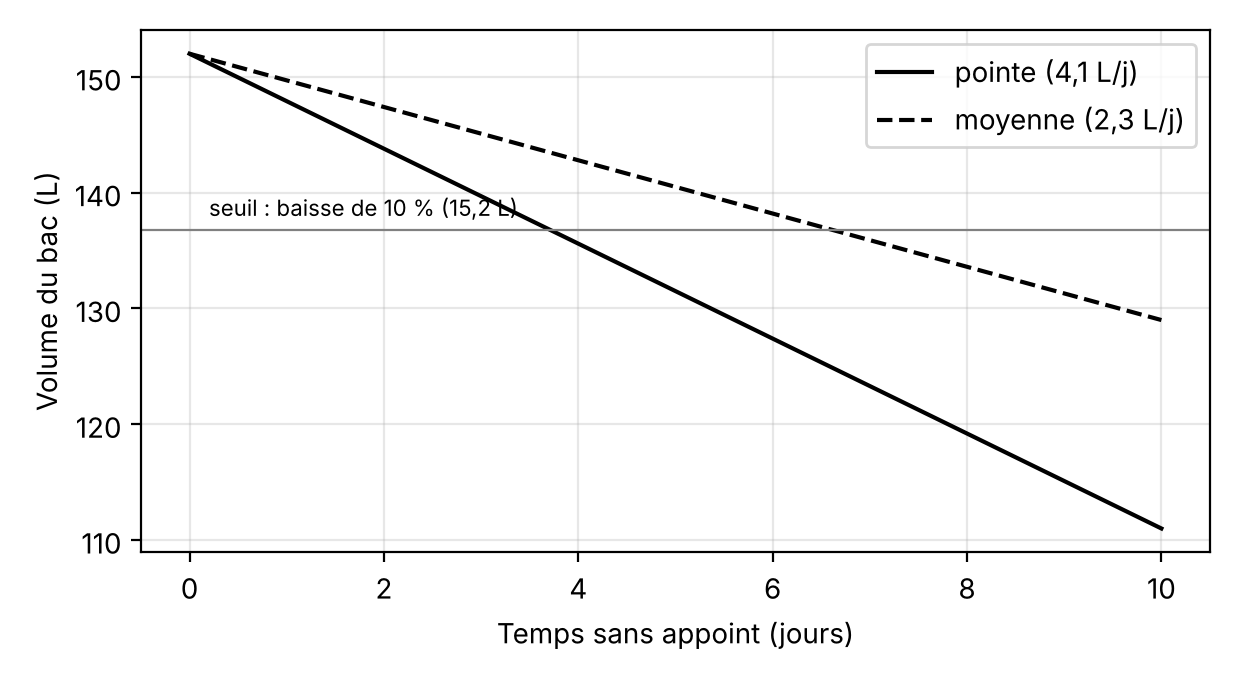
\includegraphics[width=0.78\textwidth]{img/bilan.png}
\caption{Volume du bac sans appoint, en pointe de consommation et en moyenne de cycle.}
\end{figure}

\naturecalc{théorie, avec les dimensions mesurées sur la tour (bac, flexible, tube) et des valeurs de fiches techniques ; aucun débit ni aucune consommation n'est mesuré}
\begin{demonstration}[effet d'une absence de deux semaines]
\resultat{EC_{14} \approx \qty{2,25}{mS/cm}}
Je note $V_{14}$ le volume consommé en $\qty{14}{j}$. En pointe :
\begin{align*}
V_{14} &= \qty{14}{j}\times\qty{4,1}{L/j}\\
V_{14} &= \qty{57,4}{L}
\end{align*}
En moyenne :
\begin{align*}
V_{14} &= \qty{14}{j}\times\qty{2,3}{L/j}\\
V_{14} &= \qty{32,2}{L}
\end{align*}
En pointe, il reste dans le bac $\qty{152}{L} - \qty{57,4}{L} = \qty{94,6}{L}$, soit une baisse de 38 \%. Dans le pire cas, les plants boivent l'eau sans prélever d'engrais : la même quantité de sels se retrouve dans un volume plus petit. La conductivité $EC$, en millisiemens par centimètre, est proportionnelle à la concentration en sels, donc inversement proportionnelle au volume :
\begin{align*}
EC_{14} &= EC_0\times\frac{V}{V - V_{14}}\\
EC_{14} &= \qty{1,4}{mS/cm}\times\frac{\qty{152}{L}}{\qty{94,6}{L}}\\
EC_{14} &\approx \qty{2,25}{mS/cm}
\end{align*}
\end{demonstration}

Une absence de deux semaines sans appoint dépasse donc la tolérance de 10 \%. Elle n'est acceptable qu'en début de cycle, quand les plants sont petits, ou en remplissant le bac au maximum avant le départ. En pointe de consommation, il faut un passage pour l'appoint au moins tous les trois à quatre jours.

\newcommand{\srcl}[2]{\href{#2}{\textcolor{blue}{\underline{#1}}}}

\subsection{Les besoins des plantes au cours de leur vie}

Les hypothèses du bilan hydrique (\qty{0,15}{L/j} en moyenne et \qty{0,30}{L/j} en pointe par plant) viennent de mon estimation. Je cherche ici à les vérifier avec la littérature : combien d'eau et de nutriments une laitue consomme-t-elle entre sa mise en tour et sa récolte, et comment cette consommation évolue-t-elle ? Je commence par la durée du cycle, puis je traite l'eau, puis les nutriments. Chaque chiffre de la littérature est suivi de sa source, cliquable : un clic ouvre la page du document. Les sources sont proposées pour validation, et la liste complète est à la fin de cette sous-partie.

\subsubsection*{La durée du cycle et la taille d'une laitue}

Une laitue hydroponique passe en moyenne \qty{30}{jours} de la mise en place du plant à la récolte, pour une tête de 5 à 6 onces, soit environ \qty{140}{g} à \qty{170}{g} (source \srcl{K}{https://www.aces.edu/wp-content/uploads/2022/08/ANR-2903_GreenhouseLettuceProduction_072822L-G.pdf}). Dans une chambre de culture fermée, des laitues cultivées en hydroponie jusqu'à \qty{28}{jours} après le semis ont atteint \qty{129}{g} à \qty{183}{g} de masse fraîche par plant (source \srcl{H}{https://journals.ashs.org/downloadpdf/view/journals/jashs/119/3/article-p610.pdf}). Une étude de modélisation retient \qty{144,6}{g} par plant et un cycle de \qty{30}{jours} (source \srcl{C}{https://www.mdpi.com/1660-4601/12/6/6879}). Je garde pour la tour un cycle de \qty{32}{jours} après la mise en tour, découpé en trois stades : la reprise (jours 0 à 5), la croissance des feuilles (jours 5 à 22) et la pommaison (jours 22 à 32). C'est la durée que j'ai retenue pour le suivi des plantes (partie 13).

\subsubsection*{L'eau consommée}

Une laitue consomme très peu d'eau au début, quand elle n'a que quelques feuilles, et de plus en plus ensuite : l'évapotranspiration d'un peuplement de laitues suit la surface de feuilles, et atteint son maximum à la récolte (source \srcl{H}{https://journals.ashs.org/downloadpdf/view/journals/jashs/119/3/article-p610.pdf}). Je traduis cela par un modèle simple : la consommation par plant, notée $c$ (en litres par jour), augmente linéairement avec le temps $t$ (en jours après la mise en tour), de zéro à sa valeur finale $c_f$ au jour $T = \qty{32}{j}$.

\naturecalc{théorie, à partir de valeurs tirées de la littérature ; rien de mesuré sur la tour}
\begin{demonstration}[eau consommée par une laitue pendant son cycle]
\resultat{W(T) = \frac{c_f\,T}{2} = \qty{4,8}{L}}
Je pose $c(t) = k\,t$, avec $k$ la pente de la droite, en litres par jour et par jour. La valeur finale vaut $c_f = k\,T$, donc :
\begin{align*}
k &= \frac{c_f}{T}\\
k &= \frac{\qty{0,30}{L/j}}{\qty{32}{j}}\\
k &= \qty{0,009375}{L/j^2}
\end{align*}
Le volume d'eau consommé entre le jour $0$ et le jour $t$, noté $W(t)$ en litres, est l'aire sous la droite, c'est-à-dire l'intégrale de $c$ :
\begin{align*}
W(t) &= \int_0^{t} k\,s\,\mathrm{d}s\\
W(t) &= \frac{k\,t^{2}}{2}
\end{align*}
En $t = T$, en remplaçant $k$ par $c_f/T$ :
\begin{align*}
W(T) &= \frac{c_f}{T}\times\frac{T^{2}}{2}\\
W(T) &= \frac{c_f\,T}{2}\\
W(T) &= \frac{\qty{0,30}{L/j}\times\qty{32}{j}}{2}\\
W(T) &= \qty{4,8}{L}
\end{align*}
La consommation moyenne sur le cycle est donc $W(T)/T = c_f/2 = \qty{0,15}{L/j}$ : c'est exactement mon hypothèse de départ, la moitié de la valeur de pointe.
\end{demonstration}

Je calcule maintenant ce que boit la laitue à chaque stade. À la fin de chaque stade, la consommation vaut $c = k\,t$ et le volume cumulé vaut $W = k\,t^{2}/2$.

\naturecalc{théorie, à partir de valeurs tirées de la littérature ; rien de mesuré sur la tour}
\begin{demonstration}[eau consommée à chaque stade]
\resultat{W_1 \approx \qty{0,12}{L},\quad W_2 \approx \qty{2,15}{L},\quad W_3 \approx \qty{2,53}{L}}
Avec $k = \qty{0,009375}{L/j^2}$, aux jours $t = 5$, $22$ et $32$ :
\begin{align*}
W(5) &= \frac{\qty{0,009375}{L/j^2}\times(\qty{5}{j})^{2}}{2} = \frac{\qty{0,009375}{L/j^2}\times\qty{25}{j^2}}{2} \approx \qty{0,117}{L}\\
W(22) &= \frac{\qty{0,009375}{L/j^2}\times(\qty{22}{j})^{2}}{2} = \frac{\qty{0,009375}{L/j^2}\times\qty{484}{j^2}}{2} \approx \qty{2,269}{L}\\
W(32) &= \frac{\qty{0,009375}{L/j^2}\times(\qty{32}{j})^{2}}{2} = \frac{\qty{0,009375}{L/j^2}\times\qty{1024}{j^2}}{2} = \qty{4,8}{L}
\end{align*}
Le volume de chaque stade est la différence des volumes cumulés :
\begin{align*}
W_1 &= W(5) - W(0) \approx \qty{0,117}{L} - \qty{0}{L} = \qty{0,117}{L}\\
W_2 &= W(22) - W(5) \approx \qty{2,269}{L} - \qty{0,117}{L} = \qty{2,152}{L}\\
W_3 &= W(32) - W(22) \approx \qty{4,8}{L} - \qty{2,269}{L} = \qty{2,531}{L}
\end{align*}
Les consommations en fin de stade valent $c(5) = \qty{0,009375}{L/j^2}\times\qty{5}{j} \approx \qty{0,047}{L/j}$ et $c(22) = \qty{0,009375}{L/j^2}\times\qty{22}{j} \approx \qty{0,206}{L/j}$.
\end{demonstration}

Le tableau suivant donne l'eau consommée par une laitue à chaque stade, avec un modèle linéaire.

\begin{table}[H]
\centering
\small
\renewcommand{\arraystretch}{1.1}
\begin{tabularx}{\textwidth}{|>{\raggedright\arraybackslash}p{4.4cm}|Y|Y|Y|Y|}
\hline
\textbf{Stade} & \textbf{Jours} & \textbf{$c$ en fin de stade (\unit{L/j})} & \textbf{Eau du stade (\unit{L})} & \textbf{Part du cycle} \\
\hline
Reprise & 0 à 5 & 0,047 & 0,12 & \qty{2}{\percent} \\
\hline
Croissance des feuilles & 5 à 22 & 0,206 & 2,15 & \qty{45}{\percent} \\
\hline
Pommaison & 22 à 32 & 0,300 & 2,53 & \qty{53}{\percent} \\
\hline
\textbf{Cycle entier} & 0 à 32 & 0,300 & \textbf{4,80} & \qty{100}{\percent} \\
\hline
\end{tabularx}
\caption{Eau consommée par une laitue à chaque stade (modèle linéaire, valeurs de calcul).}
\end{table}

Plus de la moitié de l'eau est bue pendant les dix derniers jours : c'est là que la tour demande le plus au bac, et c'est donc le cas que je retiens pour dimensionner l'appoint. Pour les 12 plants, le cycle consomme $12 \times \qty{4,8}{L} = \qty{57,6}{L}$, auxquels s'ajoutent $\qty{32}{j} \times \qty{0,5}{L/j} = \qty{16}{L}$ d'évaporation, soit \qty{73,6}{L}, environ la moitié du volume du bac de \qty{152}{L}.

Je compare ce modèle à la littérature. Pour une laitue de \qty{150}{g} à \qty{250}{g} en hydroponie, la solution consommée va de \qty{3}{L} à \qty{6}{L} par plant, et une laitue de \qty{200}{g} en consomme environ \qty{3}{L} à \qty{4}{L}, à Hawaï, un climat tropical proche de celui de la Polynésie (source \srcl{J}{https://www.ctahr.hawaii.edu/Hawaii/downloads/Three_Non-circulating_Hydroponic_Methods_for_Growing_lettuce.pdf}). La modélisation de la source \srcl{C}{https://www.mdpi.com/1660-4601/12/6/6879} donne \qty{20}{L} d'eau par kilogramme de laitue : pour une tête de \qty{0,1446}{kg}, cela fait $\qty{20}{L/kg}\times\qty{0,1446}{kg} \approx \qty{2,9}{L}$ par plant. Enfin, à pleine canopée, le peuplement de la source \srcl{H}{https://journals.ashs.org/downloadpdf/view/journals/jashs/119/3/article-p610.pdf} évapotranspire environ \qty{4}{L/(m^2.j)} ; comme il compte environ 18 à 19 plants par mètre carré (surface de \qty{20}{m^2} supposée), cela fait $\qty{4}{L/(m^2.j)}$ divisés par 19 plants par mètre carré, soit $\qty{4}{L/(m^2.j)}/19 \approx \qty{0,21}{L/j}$ par plant au moment de la récolte. Mon modèle (\qty{4,8}{L} par cycle et \qty{0,30}{L/j} à la fin) est donc dans la fourchette haute de la littérature, ce qui est volontaire : une hypothèse trop forte sur la consommation d'eau protège le dimensionnement de l'appoint, alors qu'une hypothèse trop faible le mettrait en défaut.

\subsubsection*{Les nutriments consommés}

Une laitue prélève surtout de l'azote (N), du phosphore (P) et du potassium (K), et beaucoup moins de calcium (Ca) et de magnésium (Mg). Une étude brésilienne qui a suivi la croissance de laitues hydroponiques pendant \qty{30}{jours} après la mise en place mesure, à la fin, \qty{295,4}{mg} d'azote, \qty{31,9}{mg} de phosphore et \qty{641,7}{mg} de potassium par plant (source \srcl{L}{https://doaj.org/article/3cad1b7f657c4b9897b2eca48a74d30d}). Pour le calcium et le magnésium, la source \srcl{H}{https://journals.ashs.org/downloadpdf/view/journals/jashs/119/3/article-p610.pdf} donne les concentrations dans les feuilles, ce qui permet de recalculer une quantité par plant à partir de la masse sèche.

\naturecalc{théorie, à partir de valeurs tirées de la littérature ; rien de mesuré sur la tour}
\begin{demonstration}[nutriments contenus dans une laitue à la récolte]
\resultat{m_{N} \approx \qty{383}{mg},\quad m_{P} \approx \qty{32}{mg},\quad m_{K} \approx \qty{1294}{mg},\quad m_{Ca} \approx \qty{79}{mg},\quad m_{Mg} \approx \qty{25}{mg}}
Pour un élément, la masse $m$ contenue dans une plante, en milligrammes, est la concentration $x$ de cet élément dans la matière sèche, en milligrammes par gramme, multipliée par la masse sèche $M_s$ de la plante, en grammes :
\begin{align*}
m &= x \times M_s
\end{align*}
La source \srcl{H}{https://journals.ashs.org/downloadpdf/view/journals/jashs/119/3/article-p610.pdf} donne $M_s = \qty{8,8}{g}$ par plant (pour \qty{183}{g} de masse fraîche) et, pour les concentrations, \qty{43500}{\micro g/g} d'azote, \qty{3630}{\micro g/g} de phosphore, \qty{147000}{\micro g/g} de potassium, \qty{9000}{\micro g/g} de calcium et \qty{2890}{\micro g/g} de magnésium. Comme $\qty{1}{mg} = \qty{1000}{\micro g}$, on a par exemple $\qty{43500}{\micro g/g} = \qty{43,5}{mg/g}$. Je calcule élément par élément :
\begin{align*}
m_{N} &= \qty{43,5}{mg/g}\times\qty{8,8}{g} \approx \qty{383}{mg}\\
m_{P} &= \qty{3,63}{mg/g}\times\qty{8,8}{g} \approx \qty{31,9}{mg}\\
m_{K} &= \qty{147}{mg/g}\times\qty{8,8}{g} \approx \qty{1294}{mg}\\
m_{Ca} &= \qty{9,0}{mg/g}\times\qty{8,8}{g} \approx \qty{79,2}{mg}\\
m_{Mg} &= \qty{2,89}{mg/g}\times\qty{8,8}{g} \approx \qty{25,4}{mg}
\end{align*}
Ce sont des estimations : les concentrations viennent des feuilles et d'un autre cultivar que celui de la tour.
\end{demonstration}

Les deux sources donnent le même ordre de grandeur pour l'azote et la même valeur pour le phosphore ; elles diffèrent d'un facteur deux pour le potassium, ce qui n'a rien d'étonnant entre deux cultivars et deux systèmes. Je retiens donc une fourchette. Pour 12 plants, et en divisant par les \qty{30}{jours} de l'étude brésilienne, on obtient les besoins suivants.

\begin{table}[H]
\centering
\small
\renewcommand{\arraystretch}{1.1}
\begin{tabularx}{\textwidth}{|>{\raggedright\arraybackslash}p{2.6cm}|Y|Y|Y|}
\hline
\textbf{Élément} & \textbf{Par plant, sur le cycle (\unit{mg})} & \textbf{Par plant, par jour (\unit{mg/j})} & \textbf{12 plants, sur le cycle (\unit{g})} \\
\hline
Azote (N) & 295 à 383 & 9,8 à 12,8 & 3,5 à 4,6 \\
\hline
Phosphore (P) & 32 & 1,1 & 0,38 \\
\hline
Potassium (K) & 642 à 1294 & 21 à 43 & 7,7 à 15,5 \\
\hline
Calcium (Ca) & 79 & 2,6 & 0,95 \\
\hline
Magnésium (Mg) & 25 & 0,85 & 0,31 \\
\hline
\end{tabularx}
\caption{Nutriments prélevés par une laitue sur un cycle, d'après les sources L et H, et besoins des 12 plants.}
\end{table}

Pour savoir si le bac contient assez de nutriments pour tout un cycle, je compare ces besoins à ce que le bac contient quand la solution est bien réglée. Une étude de 2025 sur la laitue hydroponique fixe, pour la laitue Bibb, l'équilibre idéal à \qty{132}{mg/L} d'azote, \qty{35}{mg/L} de phosphore et \qty{174}{mg/L} de potassium (source \srcl{M}{https://doaj.org/article/3f4baf90f7064b70be9ff31b0bc3bfbc}).

\naturecalc{théorie, à partir de valeurs tirées de la littérature ; rien de mesuré sur la tour}
\begin{demonstration}[part des nutriments du bac prélevée par les 12 plants]
\resultat{\text{azote : } \qty{18}{\percent} \text{ à } \qty{23}{\percent}\quad\text{et potassium : } \qty{29}{\percent} \text{ à } \qty{59}{\percent}}
La masse d'un élément dans le bac, notée $m_{bac}$ en milligrammes, est sa concentration $\rho$, en milligrammes par litre, multipliée par le volume $V = \qty{152}{L}$ :
\begin{align*}
m_{bac} &= \rho\times V\\
m_{bac,N} &= \qty{132}{mg/L}\times\qty{152}{L} = \qty{20064}{mg}\\
m_{bac,P} &= \qty{35}{mg/L}\times\qty{152}{L} = \qty{5320}{mg}\\
m_{bac,K} &= \qty{174}{mg/L}\times\qty{152}{L} = \qty{26448}{mg}
\end{align*}
La part prélevée par les 12 plants est le rapport de leur besoin au contenu du bac. Pour l'azote, avec les valeurs non arrondies \qty{3545}{mg} (environ \qty{3,5}{g}) et \qty{4594}{mg} (environ \qty{4,6}{g}) :
\begin{align*}
\frac{\qty{3545}{mg}}{\qty{20064}{mg}} &\approx \qty{17,7}{\percent}\\
\frac{\qty{4594}{mg}}{\qty{20064}{mg}} &\approx \qty{22,9}{\percent}
\end{align*}
Pour le phosphore, $\qty{383}{mg}/\qty{5320}{mg} \approx \qty{7,2}{\percent}$. Pour le potassium, avec $\qty{7700}{mg}$ et $\qty{15523}{mg}$ :
\begin{align*}
\frac{\qty{7700}{mg}}{\qty{26448}{mg}} &\approx \qty{29,1}{\percent}\\
\frac{\qty{15523}{mg}}{\qty{26448}{mg}} &\approx \qty{58,7}{\percent}
\end{align*}
\end{demonstration}

Le bac de \qty{152}{L} contient donc, quand il est bien réglé, beaucoup plus d'éléments nutritifs que les 12 plants n'en prélèvent en un cycle : de \qty{7}{\percent} à \qty{59}{\percent} selon l'élément. Ce résultat concorde avec une étude de l'université de Floride sur la laitue en film nutritif : seule une petite fraction des éléments apportés finit dans la plante (\qty{12,1}{\percent} de l'azote, \qty{12,6}{\percent} du phosphore, \qty{20,3}{\percent} du potassium), et les teneurs en azote, phosphore et calcium de la solution étaient plus élevées en fin d'essai qu'au début (source \srcl{N}{https://edis.ifas.ufl.edu/publication/AE610/pdf}). Cela a deux conséquences pour la tour. D'abord, le dosage ne sert pas à reconstituer la totalité des nutriments consommés : il corrige de petites dérives de l'EC, ce qui explique les doses de quelques millilitres des pompes -M2 et -M3. Ensuite, la conductivité monte surtout quand l'eau disparaît (consommation et évaporation) et que les sels restent : c'est le phénomène que j'étudie dans la sous-partie suivante.

\begin{aretenir}
Une laitue boit environ \qty{4,8}{L} d'eau pendant son cycle de \qty{32}{jours}, plus de la moitié pendant les dix derniers jours, et prélève de l'ordre de \qty{300}{mg} à \qty{400}{mg} d'azote, \qty{32}{mg} de phosphore et \qty{640}{mg} à \qty{1300}{mg} de potassium. Ces valeurs viennent de la littérature (cultivars et systèmes différents du mien) : elles donnent l'ordre de grandeur, et seules les mesures de la tour les confirmeront.
\end{aretenir}

\subsection{Pourquoi je n'ajoute pas de bac de secours}

Dans la première version de l'étude, la tour comportait un bac de secours d'eau claire, une pompe d'appoint (P5) et un second ruban de niveau pour remplir le bac principal automatiquement. Dans la version actuelle, j'ai supprimé ces trois éléments : l'appoint se fait à la main, avec un seau. Je justifie ici ce choix, parce qu'un bac de secours paraît de bon sens : il faut regarder ce qu'il apporte réellement, et ce qu'il coûte.

\subsubsection*{Ce qu'un bac de secours résoudrait}

Un bac de secours ne résout qu'un seul problème : le bac principal baisse de niveau et sa solution se concentre quand personne ne peut ajouter d'eau. La question est donc de savoir combien de temps la tour tient sans appoint. Dans le pire cas (les plants boivent l'eau mais ne prélèvent pas de sels, comme dans la sous-partie précédente), la conductivité vaut $EC = EC_0\,V/(V - V_c)$, avec $V_c$ le volume consommé. J'impose une limite à cette conductivité et j'en déduis la durée. Je prends deux limites : le haut de la plage cible de la laitue, \qty{1,8}{mS/cm}, et le seuil d'alarme du dashboard, \qty{2,2}{mS/cm} (à partir duquel la laitue risque des pointes brûlées).

\naturecalc{théorie, avec les dimensions mesurées sur la tour (bac, flexible, tube) et des valeurs de fiches techniques ; aucun débit ni aucune consommation n'est mesuré}
\begin{demonstration}[durée sans appoint selon la conductivité tolérée]
\resultat{T = \frac{V}{C}\left(1 - \frac{EC_0}{EC_{lim}}\right)}
Je pars de la relation $EC_{lim} = EC_0\,V/(V - V_c)$, où $EC_0 = \qty{1,4}{mS/cm}$ est la conductivité de départ, $EC_{lim}$ la limite tolérée, $V = \qty{152}{L}$ le volume du bac et $V_c$ le volume consommé, en litres. Je l'isole ligne par ligne :
\begin{align*}
EC_{lim}\,(V - V_c) &= EC_0\,V\\
V - V_c &= V\,\frac{EC_0}{EC_{lim}}\\
V_c &= V\left(1 - \frac{EC_0}{EC_{lim}}\right)
\end{align*}
La consommation journalière $C$ étant constante (en litres par jour), $V_c = C\,T$, d'où le résultat. Pour la limite de \qty{1,8}{mS/cm} :
\begin{align*}
V_c &= \qty{152}{L}\times\left(1 - \frac{\qty{1,4}{mS/cm}}{\qty{1,8}{mS/cm}}\right)\\
V_c &= \qty{152}{L}\times0{,}2222\\
V_c &\approx \qty{33,8}{L}
\end{align*}
\begin{align*}
T_{pic} &= \frac{\qty{33,8}{L}}{\qty{4,1}{L/j}} \approx \qty{8,2}{j}\\
T_{moy} &= \frac{\qty{33,8}{L}}{\qty{2,3}{L/j}} \approx \qty{14,7}{j}
\end{align*}
Pour la limite de \qty{2,2}{mS/cm} :
\begin{align*}
V_c &= \qty{152}{L}\times\left(1 - \frac{\qty{1,4}{mS/cm}}{\qty{2,2}{mS/cm}}\right)\\
V_c &= \qty{152}{L}\times0{,}3636\\
V_c &\approx \qty{55,3}{L}
\end{align*}
\begin{align*}
T_{pic} &= \frac{\qty{55,3}{L}}{\qty{4,1}{L/j}} \approx \qty{13,5}{j}\\
T_{moy} &= \frac{\qty{55,3}{L}}{\qty{2,3}{L/j}} \approx \qty{24,0}{j}
\end{align*}
\end{demonstration}

Les trois critères donnent donc les autonomies suivantes, sans aucun appoint.

\begin{table}[H]
\centering
\small
\renewcommand{\arraystretch}{1.1}
\begin{tabularx}{\textwidth}{|>{\raggedright\arraybackslash}p{6.4cm}|Y|Y|}
\hline
\textbf{Critère} & \textbf{En pointe (\unit{j})} & \textbf{En moyenne (\unit{j})} \\
\hline
Baisse de \qty{10}{\percent} du volume (prudent) & 3,7 & 6,6 \\
\hline
$EC$ atteint \qty{1,8}{mS/cm} (haut de la plage cible) & 8,2 & 14,7 \\
\hline
$EC$ atteint \qty{2,2}{mS/cm} (alarme) & 13,5 & 24,0 \\
\hline
\end{tabularx}
\caption{Durée sans appoint selon le critère retenu, avec $EC_0 = \qty{1,4}{mS/cm}$.}
\end{table}

\naturecalc{théorie, avec les dimensions mesurées sur la tour (bac, flexible, tube) et des valeurs de fiches techniques ; aucun débit ni aucune consommation n'est mesuré}
\begin{demonstration}[conductivité après une absence d'une semaine ou de deux semaines]
\resultat{EC_{7} \approx \qty{1,73}{mS/cm}\quad\text{et}\quad EC_{14} \approx \qty{2,09}{mS/cm}}
Une semaine entièrement en pointe consomme $V_c = \qty{7}{j}\times\qty{4,1}{L/j} = \qty{28,7}{L}$. Avec la relation $EC = EC_0\,V/(V - V_c)$ :
\begin{align*}
EC_{7} &= \qty{1,4}{mS/cm}\times\frac{\qty{152}{L}}{\qty{152}{L} - \qty{28,7}{L}}\\
EC_{7} &= \qty{1,4}{mS/cm}\times\frac{\qty{152}{L}}{\qty{123,3}{L}}\\
EC_{7} &\approx \qty{1,73}{mS/cm}
\end{align*}
La pointe ne dure que les dix derniers jours du cycle. Deux semaines au pire moment du cycle comptent donc au plus dix jours de pointe et quatre jours de consommation moyenne :
\begin{align*}
V_c &= \qty{10}{j}\times\qty{4,1}{L/j} + \qty{4}{j}\times\qty{2,3}{L/j}\\
V_c &= \qty{41,0}{L} + \qty{9,2}{L} = \qty{50,2}{L}
\end{align*}
\begin{align*}
EC_{14} &= \qty{1,4}{mS/cm}\times\frac{\qty{152}{L}}{\qty{152}{L} - \qty{50,2}{L}}\\
EC_{14} &= \qty{1,4}{mS/cm}\times\frac{\qty{152}{L}}{\qty{101,8}{L}}\\
EC_{14} &\approx \qty{2,09}{mS/cm}
\end{align*}
\end{demonstration}

Même dans le pire cas, une absence d'une semaine laisse la conductivité dans la plage cible (\qty{1,73}{mS/cm}, sous \qty{1,8}{mS/cm}), et une absence de deux semaines, au pire moment du cycle, reste sous le seuil d'alarme (\qty{2,09}{mS/cm}, sous \qty{2,2}{mS/cm}). La règle de \qty{10}{\percent} de la sous-partie précédente est donc très prudente : elle fixe la fréquence confortable des passages, pas la limite de ce que la tour supporte. Et ce calcul prend le pire cas, où les plants ne prélèvent aucun sel : en réalité, ils en prélèvent une partie, et la conductivité monte moins vite.

\subsubsection*{Pourquoi cela ne justifie pas un bac de secours}

Un bac de secours de volume $V_s$ allonge l'autonomie de $V_s/C$ : avec \qty{40}{L}, cela fait $\qty{40}{L}/\qty{4,1}{L/j} \approx \qty{9,8}{j}$ en pointe. Mais ce bac de secours doit lui-même être rempli à la main, et c'est là son premier défaut : il ne supprime pas le geste d'aller chercher de l'eau, il le repousse. Or ce geste est léger. En pointe, la tour consomme \qty{4,1}{L/j}, soit un seau de \qty{10}{L} tous les deux jours et demi, ou trois seaux par semaine. Et la tour est visitée, puisque je mesure, je règle et j'entretiens : le projet est un démonstrateur suivi régulièrement, pas un système laissé seul plusieurs semaines.

Le deuxième défaut est la fiabilité. Un remplissage automatique ajoute des pannes possibles : un ruban de niveau qui se décale, une pompe d'appoint qui reste enclenchée ou qui ne démarre plus. Une pompe bloquée en marche remplit le bac jusqu'au débordement, car le système n'a aucun moyen d'évacuer l'excédent, et le bac contient une solution nutritive qu'il ne faut pas rejeter. Un ruban faussé qui déclenche trop d'appoint dilue la solution : le dosage ne sait pas retirer de l'eau, il ne sait qu'ajouter des engrais. Avec l'appoint manuel, c'est une personne qui décide, et elle regarde le niveau et la conductivité avant d'ajouter de l'eau.

Le troisième défaut est le nombre de pièces. Le bac de secours demande un second réservoir, une pompe, un second ruban de niveau avec son entrée sur le convertisseur analogique-numérique, une sortie de la carte MOSFET\ix{15}, un fusible, des câbles, du programme et des essais en plus : chacun de ces éléments est à acheter, à câbler et à tester, dans un projet où je dois condenser trois années de formation en trois mois. Il touche aussi le bilan d'énergie : j'ai retiré la pompe d'appoint du bilan de la partie 5, où chaque wattheure compte pour que le panneau et les batteries restent dimensionnés avec une marge.

Enfin, le système protège déjà ce que le bac de secours protégerait. Quand le réservoir passe sous \qty{15}{\percent}, le pilote arrête la pompe et le dosage et lève une alarme « ajouter de l'eau » (partie 8.4), et, dans la première version du programme (partie 8.12), l'Arduino coupait lui-même la circulation sous le seuil de niveau. Dans la version actuelle, cette décision est prise par le Raspberry, et la coupure de l'Arduino après \qty{30}{s} de silence ne mesure pas le niveau : une protection locale contre la marche à sec reste à ajouter dans l'Arduino (partie 8.3). Quand la conductivité devient trop haute, la règle de décision du pilote recommande d'ajouter de l'eau claire. La tour s'arrête donc dans un état sûr, et le dashboard me prévient : la seule chose qu'elle ne fait pas est de se remplir toute seule.

\begin{aretenir}
Sans aucun appoint, la tour tient au moins une semaine au pire moment du cycle dans la plage cible de conductivité (\qty{1,73}{mS/cm}) et deux semaines sous le seuil d'alarme (\qty{2,09}{mS/cm}). Un bac de secours ne ferait que repousser le remplissage à la main, ajouterait des pannes possibles (débordement, dilution) et des pièces à acheter, câbler et tester, et alourdirait le bilan d'énergie. Je garde donc un bac unique et un appoint manuel, avec un passage tous les trois à quatre jours en pointe. Je reconsidérerai ce choix si la tour devait rester sans visite plus de deux semaines pendant la pointe : un remplissage par flotteur mécanique, sans pompe, serait alors la première solution à étudier.
\end{aretenir}

\subsubsection*{Sources de cette sous-partie}

Les sources C, H, J, K, L, M et N de cette sous-partie sont dans la bibliographie, à la toute fin du rapport. Dans le texte, chaque lettre est un lien cliquable vers la page de la source.

\subsection{Protocole de mesure}

Aucune mesure n'est encore faite : tout ce qui précède vient de la fiche de la pompe, du plan du couvercle et d'hypothèses. Les mesures suivantes permettront de remplacer les hypothèses par des valeurs réelles. Pour toutes, il faut un seau gradué de \qty{10}{L}, un chronomètre et un mètre ruban.

Pour le \textbf{débit réel de la pompe}, je garde le circuit complet (couvercle répartiteur en place, flexible raccordé), car c'est le point de fonctionnement calculé. Je place le seau gradué au pied de la tour et je recueille toute l'eau qui retombe de la paroi. Je démarre la pompe, j'attends \qty{10}{s} que le débit se stabilise, puis je lance le chronomètre et je l'arrête quand le seau atteint \qty{10}{L}. Je reverse l'eau dans le bac et je recommence cinq fois. Un second essai, flexible débranché du couvercle et sortie à \qty{1,2}{m} au-dessus de l'eau, donne le débit sans les pertes du couvercle et permet de les isoler. Le débit en litres par heure est $Q = 3600\,V_s/t$, avec $V_s$ le volume du seau, en litres, et $t$ la durée, en secondes. La valeur attendue est \qty{388}{L/h}.

Pour la \textbf{hauteur du jet}, je retire le couvercle, j'oriente l'extrémité du flexible vers le haut et je fixe un mètre ruban à la verticale. Je photographie le jet cinq fois et je relève sa hauteur maximale. Sans frottement de l'air, elle devrait être proche de \qty{15}{cm} pour l'ensemble des huit trous ; avec le flexible seul, la hauteur dépend de la section de sortie, donc cette mesure sert surtout à comparer deux essais entre eux.

Pour la \textbf{répartition de l'eau}, qui est la difficulté de départ, je fais tourner la pompe avec le couvercle en place et je regarde la paroi : les huit zones arrosées doivent se rejoindre, sans zone sèche entre elles. Je note aussi le nombre de godets dont les racines sont mouillées.

Pour la \textbf{consommation d'eau}, je colle une règle graduée verticale dans le bac. Chaque jour à la même heure, pompe arrêtée depuis plus de cinq minutes, je relève la hauteur d'eau, et je note les appoints mesurés au seau. Après au moins sept jours, la pente de la droite du niveau en fonction du temps donne la consommation en litres par jour, à comparer à \qty{2,3}{L/j} en moyenne et \qty{4,1}{L/j} en pointe.

\begin{aretenir}
La pompe de \qty{800}{L/h} débite environ \qty{388}{L/h} dans le circuit, sous \qty{2,57}{m} : c'est le flexible de \qty{9}{mm} qui limite le débit, non le couvercle. Le débit moyen est d'environ \qty{32}{L/h} par plant, soit 16 fois le besoin minimal retenu (à confirmer par la mesure de répartition), et le bac de \qty{152}{L} se renouvelle en \qty{23,5}{min}. Le bac consomme \qty{2,3}{L/j} en moyenne et \qty{4,1}{L/j} en pointe : il faut un appoint d'environ \qty{15}{L} tous les quatre jours en pointe. Ces chiffres sont théoriques tant que les mesures ne sont pas faites.
\end{aretenir}



% =====================================================================
\clearpage
\partieENO{La mécanique}

Cette partie regarde la tour comme un objet qui doit tenir debout, porter l'eau et les plantes, et résister au vent. Je commence par la structure et ses masses. Je calcule ensuite la disposition des 12 trous de plantation. Je termine par la stabilité : le vent peut-il renverser la tour, et que faire quand le bac est presque vide ? Aucune dimension du bac n'a encore été mesurée avec précision : les valeurs marquées « hypothèse » sont à remplacer par des mesures.

\Needspace{8\baselineskip}\subsection{La structure et les masses}

La tour est un tube de PVC de \qty{1}{m} de haut, de diamètre extérieur \qty{159}{mm} et de diamètre intérieur \qty{144}{mm}. Il se tient dans le bac de \qty{152}{L}. Le couvercle répartiteur, imprimé en 3D en PETG, ferme le haut. Je veux connaître la masse du tube pour savoir ce que le bac doit porter.

\naturecalc{théorie (dimensions du tube mesurées ; dimensions du bac, masses et vent : hypothèses à mesurer)}
\begin{demonstration}[masse du tube de PVC]
\resultat{m_t \approx \qty{5,0}{kg}}
Je note $D_e$ le diamètre extérieur du tube, en mètres (\qty{0,159}{m}), $D_i$ son diamètre intérieur, en mètres (\qty{0,144}{m}), $H$ sa hauteur, en mètres (\qty{1}{m}), $\rho$ la masse volumique du PVC, en kg/m$^3$ (environ \qty{1400}{kg/m^3}), $A$ l'aire de la couronne de PVC, en m$^2$, et $m_t$ la masse du tube, en kg. L'aire d'un disque de diamètre $D$ vaut $\pi D^2/4$. L'aire de la couronne est la différence entre le disque extérieur et le disque intérieur :
\begin{align*}
A &= \frac{\pi D_e^2}{4} - \frac{\pi D_i^2}{4}\\
A &= \frac{\pi}{4}\left(D_e^2 - D_i^2\right)\\
A &= \frac{\pi}{4}\left((\qty{0,159}{m})^2 - (\qty{0,144}{m})^2\right)\\
A &= \frac{\pi}{4} \times \qty{0,004545}{m^2}\\
A &\approx \qty{0,00357}{m^2}
\end{align*}
Le volume du PVC est l'aire multipliée par la hauteur, et la masse est la masse volumique multipliée par le volume :
\begin{align*}
V &= A \, H = \qty{0,00357}{m^2} \times \qty{1}{m} = \qty{0,00357}{m^3}\\
m_t &= \rho \, V\\
m_t &= \qty{1400}{kg/m^3} \times \qty{0,00357}{m^3}\\
m_t &\approx \qty{5,0}{kg}
\end{align*}
J'arrondis à un chiffre après la virgule. Le volume intérieur du tube vaut $\pi D_i^2 H / 4 \approx \qty{16,3}{L}$ : c'est la place disponible pour les racines.
\end{demonstration}

Je retiens pour la suite une masse de la tour à vide de \qty{7,3}{kg}, en comptant \qty{5,0}{kg} de tube, \qty{0,3}{kg} de couvercle et \qty{2,0}{kg} de plants, de paniers et de film d'eau (hypothèses à peser). Le bac vide pèse \qty{8}{kg} (hypothèse à peser).

\Needspace{8\baselineskip}\subsection{Les trous de plantation}

La tour porte 12 plants, répartis sur 4 niveaux de 3 plants. Les trois trous d'un niveau sont à \ang{120} les uns des autres, et chaque niveau est décalé de \ang{60} par rapport au précédent, pour que les feuilles ne se gênent pas. Les niveaux sont espacés de \qty{20}{cm}. Les trous reçoivent des paniers de \qty{50}{mm} de diamètre (hypothèse, à confirmer avec les paniers achetés). Je vérifie que la paroi reste assez solide entre deux trous d'un même niveau.

\naturecalc{théorie (dimensions du tube mesurées ; dimensions du bac, masses et vent : hypothèses à mesurer)}
\begin{demonstration}[largeur de paroi restante entre deux trous]
\resultat{e \approx \qty{117}{mm}}
Je note $D_e$ le diamètre extérieur du tube, en mètres (\qty{0,159}{m}), $P_e$ son périmètre extérieur, en mètres, $n$ le nombre de trous par niveau (sans unité, ici 3), $d_t$ le diamètre d'un trou, en mètres (\qty{0,050}{m}), et $e$ la largeur de paroi pleine entre deux trous voisins, en mètres. Le périmètre d'un cercle est $\pi$ fois son diamètre :
\begin{align*}
P_e &= \pi D_e\\
P_e &= \pi \times \qty{0,159}{m}\\
P_e &\approx \qty{0,4995}{m}
\end{align*}
Les $n$ trous occupent $n\,d_t$ de ce périmètre (en comptant le trou sur l'arc extérieur). Il reste $P_e - n\,d_t$, partagé en $n$ intervalles égaux :
\begin{align*}
e &= \frac{P_e - n\,d_t}{n}\\
e &= \frac{\qty{0,4995}{m} - 3 \times \qty{0,050}{m}}{3}\\
e &= \frac{\qty{0,3495}{m}}{3}\\
e &\approx \qty{0,1165}{m}
\end{align*}
soit environ \qty{117}{mm}, en arrondissant au millimètre. La paroi pleine entre deux trous vaut plus de deux fois le diamètre d'un trou : le tube reste rigide.
\end{demonstration}

\Needspace{8\baselineskip}\subsection{La stabilité de la tour face au vent}

\subsubsection*{Ce que je cherche et ce que je suppose}

Je cherche à savoir si une rafale peut renverser le bac et la tour, et à partir de quelle quantité d'eau la tour est sûre. Le vent pousse la tour avec une force, qui crée un moment de renversement autour de l'arête basse du bac. Le poids du bac et de l'eau crée un moment inverse, qui le retient. La tour est sûre quand le moment qui retient vaut au moins deux fois celui qui renverse. Ce calcul ne concerne que la tour (tube, plants, bac et eau). Le panneau solaire porté par sa structure métallique et l'armoire électrique, placés en hauteur, offrent une surface au vent supplémentaire que je n'ai pas encore calculée : un second calcul sur l'installation complète, avec la fixation réelle au sol ou au plateau, est à faire avant de laisser le montage dehors par grand vent.

Je suppose une rafale de $v = \qty{15}{m/s}$ (environ \qty{54}{km/h}, hypothèse pour les alizés de Tahiti), une masse volumique de l'air $\rho_a = \qty{1,2}{kg/m^3}$ et un coefficient de traînée d'un cylindre $C_d = 1{,}2$. Le bac a pour largeur $b = \qty{0,40}{m}$ et pour hauteur $h_b = \qty{0,40}{m}$ (hypothèses à mesurer).

\naturecalc{théorie (dimensions du tube mesurées ; dimensions du bac, masses et vent : hypothèses à mesurer)}
\begin{demonstration}[force du vent sur le tube]
\resultat{F = \tfrac{1}{2}\,\rho_a\, C_d\, S\, v^2 \approx \qty{25,8}{N}}
Je note $F$ la force du vent, en newtons, $S$ la surface que le tube présente au vent, en m$^2$, et $v$ la vitesse du vent, en m/s. La pression dynamique d'un écoulement d'air est l'énergie cinétique par unité de volume :
\begin{align*}
q &= \frac{1}{2}\,\rho_a\, v^2
\end{align*}
Une masse d'air $m$ qui se déplace à la vitesse $v$ a l'énergie cinétique $\tfrac{1}{2} m v^2$. En divisant par son volume $V$, on obtient $\tfrac{1}{2} (m/V) v^2 = \tfrac{1}{2} \rho_a v^2$, en joules par mètre cube, c'est-à-dire en pascals. La force est cette pression, multipliée par la surface au vent et par le coefficient de traînée $C_d$ qui dit quelle part de la pression s'applique réellement sur l'objet :
\begin{align*}
F &= C_d\, S\, q = \frac{1}{2}\,\rho_a\, C_d\, S\, v^2
\end{align*}
La surface au vent d'un cylindre est son diamètre multiplié par sa hauteur :
\begin{align*}
S &= D_e \, H = \qty{0,159}{m} \times \qty{1}{m} = \qty{0,159}{m^2}
\end{align*}
Application :
\begin{align*}
F &= \frac{1}{2} \times \qty{1,2}{kg/m^3} \times 1{,}2 \times \qty{0,159}{m^2} \times (\qty{15}{m/s})^2\\
F &= \frac{1}{2} \times \qty{1,2}{kg/m^3} \times 1{,}2 \times \qty{0,159}{m^2} \times \qty{225}{m^2/s^2}\\
F &\approx \qty{25,8}{N}
\end{align*}
J'arrondis à un chiffre après la virgule. L'unité est bien le newton : $\unit{kg/m^3} \times \unit{m^2} \times \unit{m^2/s^2} = \unit{kg\,m/s^2}$.
\end{demonstration}

\naturecalc{théorie (dimensions du tube mesurées ; dimensions du bac, masses et vent : hypothèses à mesurer)}
\begin{demonstration}[moments et masse minimale]
\resultat{m_{\min} = \dfrac{4\, F\, \left(h_b + H/2\right)}{g\, b} \approx \qty{23,6}{kg}}
Je note $M_v$ le moment du vent autour de l'arête basse du bac, en N$\cdot$m, $M_p$ le moment du poids, en N$\cdot$m, $m$ la masse totale (bac, tour et eau), en kg, $g = \qty{9,81}{m/s^2}$ l'accélération de la pesanteur, et $n_s$ le coefficient de sécurité (sans unité). La force du vent s'applique au milieu du tube, à la hauteur $h_b + H/2$ au-dessus du sol, avec $H = \qty{1}{m}$. Un moment est une force multipliée par son bras de levier :
\begin{align*}
M_v &= F\left(h_b + \frac{H}{2}\right)\\
M_v &= \qty{25,8}{N} \times \left(\qty{0,40}{m} + \qty{0,50}{m}\right)\\
M_v &\approx \qty{23,2}{N\,m}
\end{align*}
Le poids $m g$ s'applique au centre du bac, à la distance $b/2$ de l'arête :
\begin{align*}
M_p &= m\, g\, \frac{b}{2}
\end{align*}
Je veux $M_p \ge n_s\, M_v$ avec $n_s = 2$. J'isole $m$ :
\begin{align*}
m\, g\, \frac{b}{2} &\ge 2\, M_v\\
m &\ge \frac{4\, M_v}{g\, b}\\
m_{\min} &= \frac{4 \times \qty{23,2}{N\,m}}{\qty{9,81}{m/s^2} \times \qty{0,40}{m}}\\
m_{\min} &\approx \qty{23,6}{kg}
\end{align*}
Le bac vide et la tour pèsent $\qty{8}{kg} + \qty{7,3}{kg} = \qty{15,3}{kg}$. Il manque donc $\qty{23,6}{kg} - \qty{15,3}{kg} \approx \qty{8,3}{kg}$, soit environ \qty{8}{L} d'eau pour atteindre la sécurité. Avec le bac plein ($m = \qty{15,3}{kg} + \qty{152}{kg} = \qty{167,3}{kg}$), le coefficient de sécurité est :
\begin{align*}
n_s &= \frac{M_p}{M_v} = \frac{\qty{167,3}{kg} \times \qty{9,81}{m/s^2} \times \qty{0,20}{m}}{\qty{23,2}{N\,m}} \approx 14
\end{align*}
\end{demonstration}

\naturecalc{théorie (dimensions du tube mesurées ; dimensions du bac, masses et vent : hypothèses à mesurer)}
\begin{demonstration}[angle de basculement du bac presque vide]
\resultat{\theta_c = \arctan\!\left(\dfrac{b/2}{h_G}\right) \approx \ang{20,5}}
Je note $h_G$ la hauteur du centre de gravité, en mètres, et $\theta_c$ l'angle d'inclinaison à partir duquel le poids passe de l'autre côté de l'arête, en degrés. Le centre de gravité est la moyenne des positions pondérées par les masses. Le bac (\qty{8}{kg}) a son centre à \qty{0,20}{m} et la tour (\qty{7,3}{kg}) à \qty{0,90}{m} (\qty{0,40}{m} de bac plus \qty{0,50}{m} de demi-tour) :
\begin{align*}
h_G &= \frac{m_b \times \qty{0,20}{m} + m_{tour} \times \qty{0,90}{m}}{m_b + m_{tour}}\\
h_G &= \frac{\qty{8}{kg} \times \qty{0,20}{m} + \qty{7,3}{kg} \times \qty{0,90}{m}}{\qty{15,3}{kg}}\\
h_G &\approx \qty{0,534}{m}
\end{align*}
Quand on incline le bac d'un angle $\theta$ autour de l'arête, le poids passe de l'autre côté quand la verticale du centre de gravité dépasse l'arête. Dans le triangle rectangle de côtés $b/2$ et $h_G$ :
\begin{align*}
\tan \theta_c &= \frac{b/2}{h_G}\\
\theta_c &= \arctan\!\left(\frac{\qty{0,20}{m}}{\qty{0,534}{m}}\right)\\
\theta_c &\approx \ang{20,5}
\end{align*}
Ce seuil est inférieur au seuil de détection de chute de l'Arduino (\ang{35}, partie 8) : un bac presque vide qui bascule est donc déjà tombé quand la sécurité se déclenche. Il vaut mieux ne jamais le laisser vide.
\end{demonstration}

\begin{aretenir}
Le tube de PVC pèse environ \qty{5,0}{kg}, et la paroi entre deux trous de plantation reste large de \qty{117}{mm}. Une rafale de \qty{15}{m/s} pousse la tour avec environ \qty{26}{N}. Le bac plein résiste largement (coefficient 14). Presque vide, il peut se renverser : il faut au moins \qty{8}{L} d'eau dedans pour garder un coefficient de 2, et lester le bac si le niveau doit descendre plus bas. Les dimensions du bac et les masses sont des hypothèses à mesurer.
\end{aretenir}


% ===== ETUDE ELECTRIQUE =====
% Partie 5 : etude electrique complete (v2)
% =====================================================================
% PARTIE 4 : L'ETUDE ELECTRIQUE (etude electrique v2, texte integral)
\clearpage
\partieENO{L'étude électrique et l'énergie solaire}

La tour fonctionne sans prise de courant : tout vient du soleil. Cette partie reprend en entier l'étude électrique (version 2) de la tour, avec ses calculs, ses démonstrations, ses tableaux et son protocole de mesure. Elle répond, dans l'ordre, à quatre questions. Combien d'énergie la tour consomme-t-elle en une journée ? Le panneau de \qty{120}{Wc} en produit-il assez le pire mois ? Les batteries tiennent-elles la nuit et quelques jours sans soleil ? Quelles sections de câbles et quels fusibles faut-il pour que le montage reste sûr ? Je commence par présenter le système (5.1) et son schéma (5.2). Je calcule ensuite la consommation (5.3), puis je dimensionne le panneau (5.4) et les batteries (5.5). Je vérifie la tension réellement présente sur le réseau \qty{12}{V} (5.6), je choisis les câbles et les fusibles (5.7), puis je décris le protocole de mesure qui remplacera les hypothèses par des valeurs réelles (5.8). Je rassemble les hypothèses (5.9) et je termine par la synthèse (5.10).

\Needspace{8\baselineskip}\subsection{Présentation du système électrique}

La tour est alimentée uniquement par le soleil. L'énergie suit le chemin suivant. Le panneau TE1250 de \qty{120}{Wc} produit l'électricité. Le régulateur MPPT\ix{19} SLC-MT2024 (SLD Tech, \qty{20}{A}) l'adapte et charge les batteries, et des fusibles protègent chaque ligne. Les batteries de \qty{12}{V} (\qty{6}{Ah} et \qty{17}{Ah}, en parallèle) stockent pour la nuit. Un convertisseur UBEC\ix{17} transforme le \qty{12}{V} en \qty{5}{V} pour le Raspberry Pi et l'Arduino. La carte de puissance Adafruit 6318, à huit MOSFET\ix{15}, commande les pompes en \qty{12}{V}. Un capteur de courant INA260\ix{22} mesure la tension et le courant de la batterie. Le synoptique et la feuille d'alimentation et de puissance sont reproduits ci-dessous (ils figurent aussi en partie 8.1) ; la partie 5.2 explique comment les lire.

Les sept fonctions sont donc : produire (panneau), réguler et protéger (régulateur MPPT\ix{19} et fusibles), stocker (batteries), mesurer l'énergie (INA260\ix{22}), convertir (UBEC\ix{17}), décider (Raspberry Pi 3 B avec son dongle Wi-Fi) et lire et agir (Arduino Uno R3, carte MOSFET\ix{15}, pompes et capteurs : pH, EC, eTape\ix{23}, DS18B20\ix{24}, DHT20\ix{24}, lumière, accéléromètre LIS3DHTR, ADS1115\ix{16}).

Le schéma synoptique suivant regroupe ces éléments en blocs et montre comment ils sont reliés.

\begin{figure}[H]
\centering
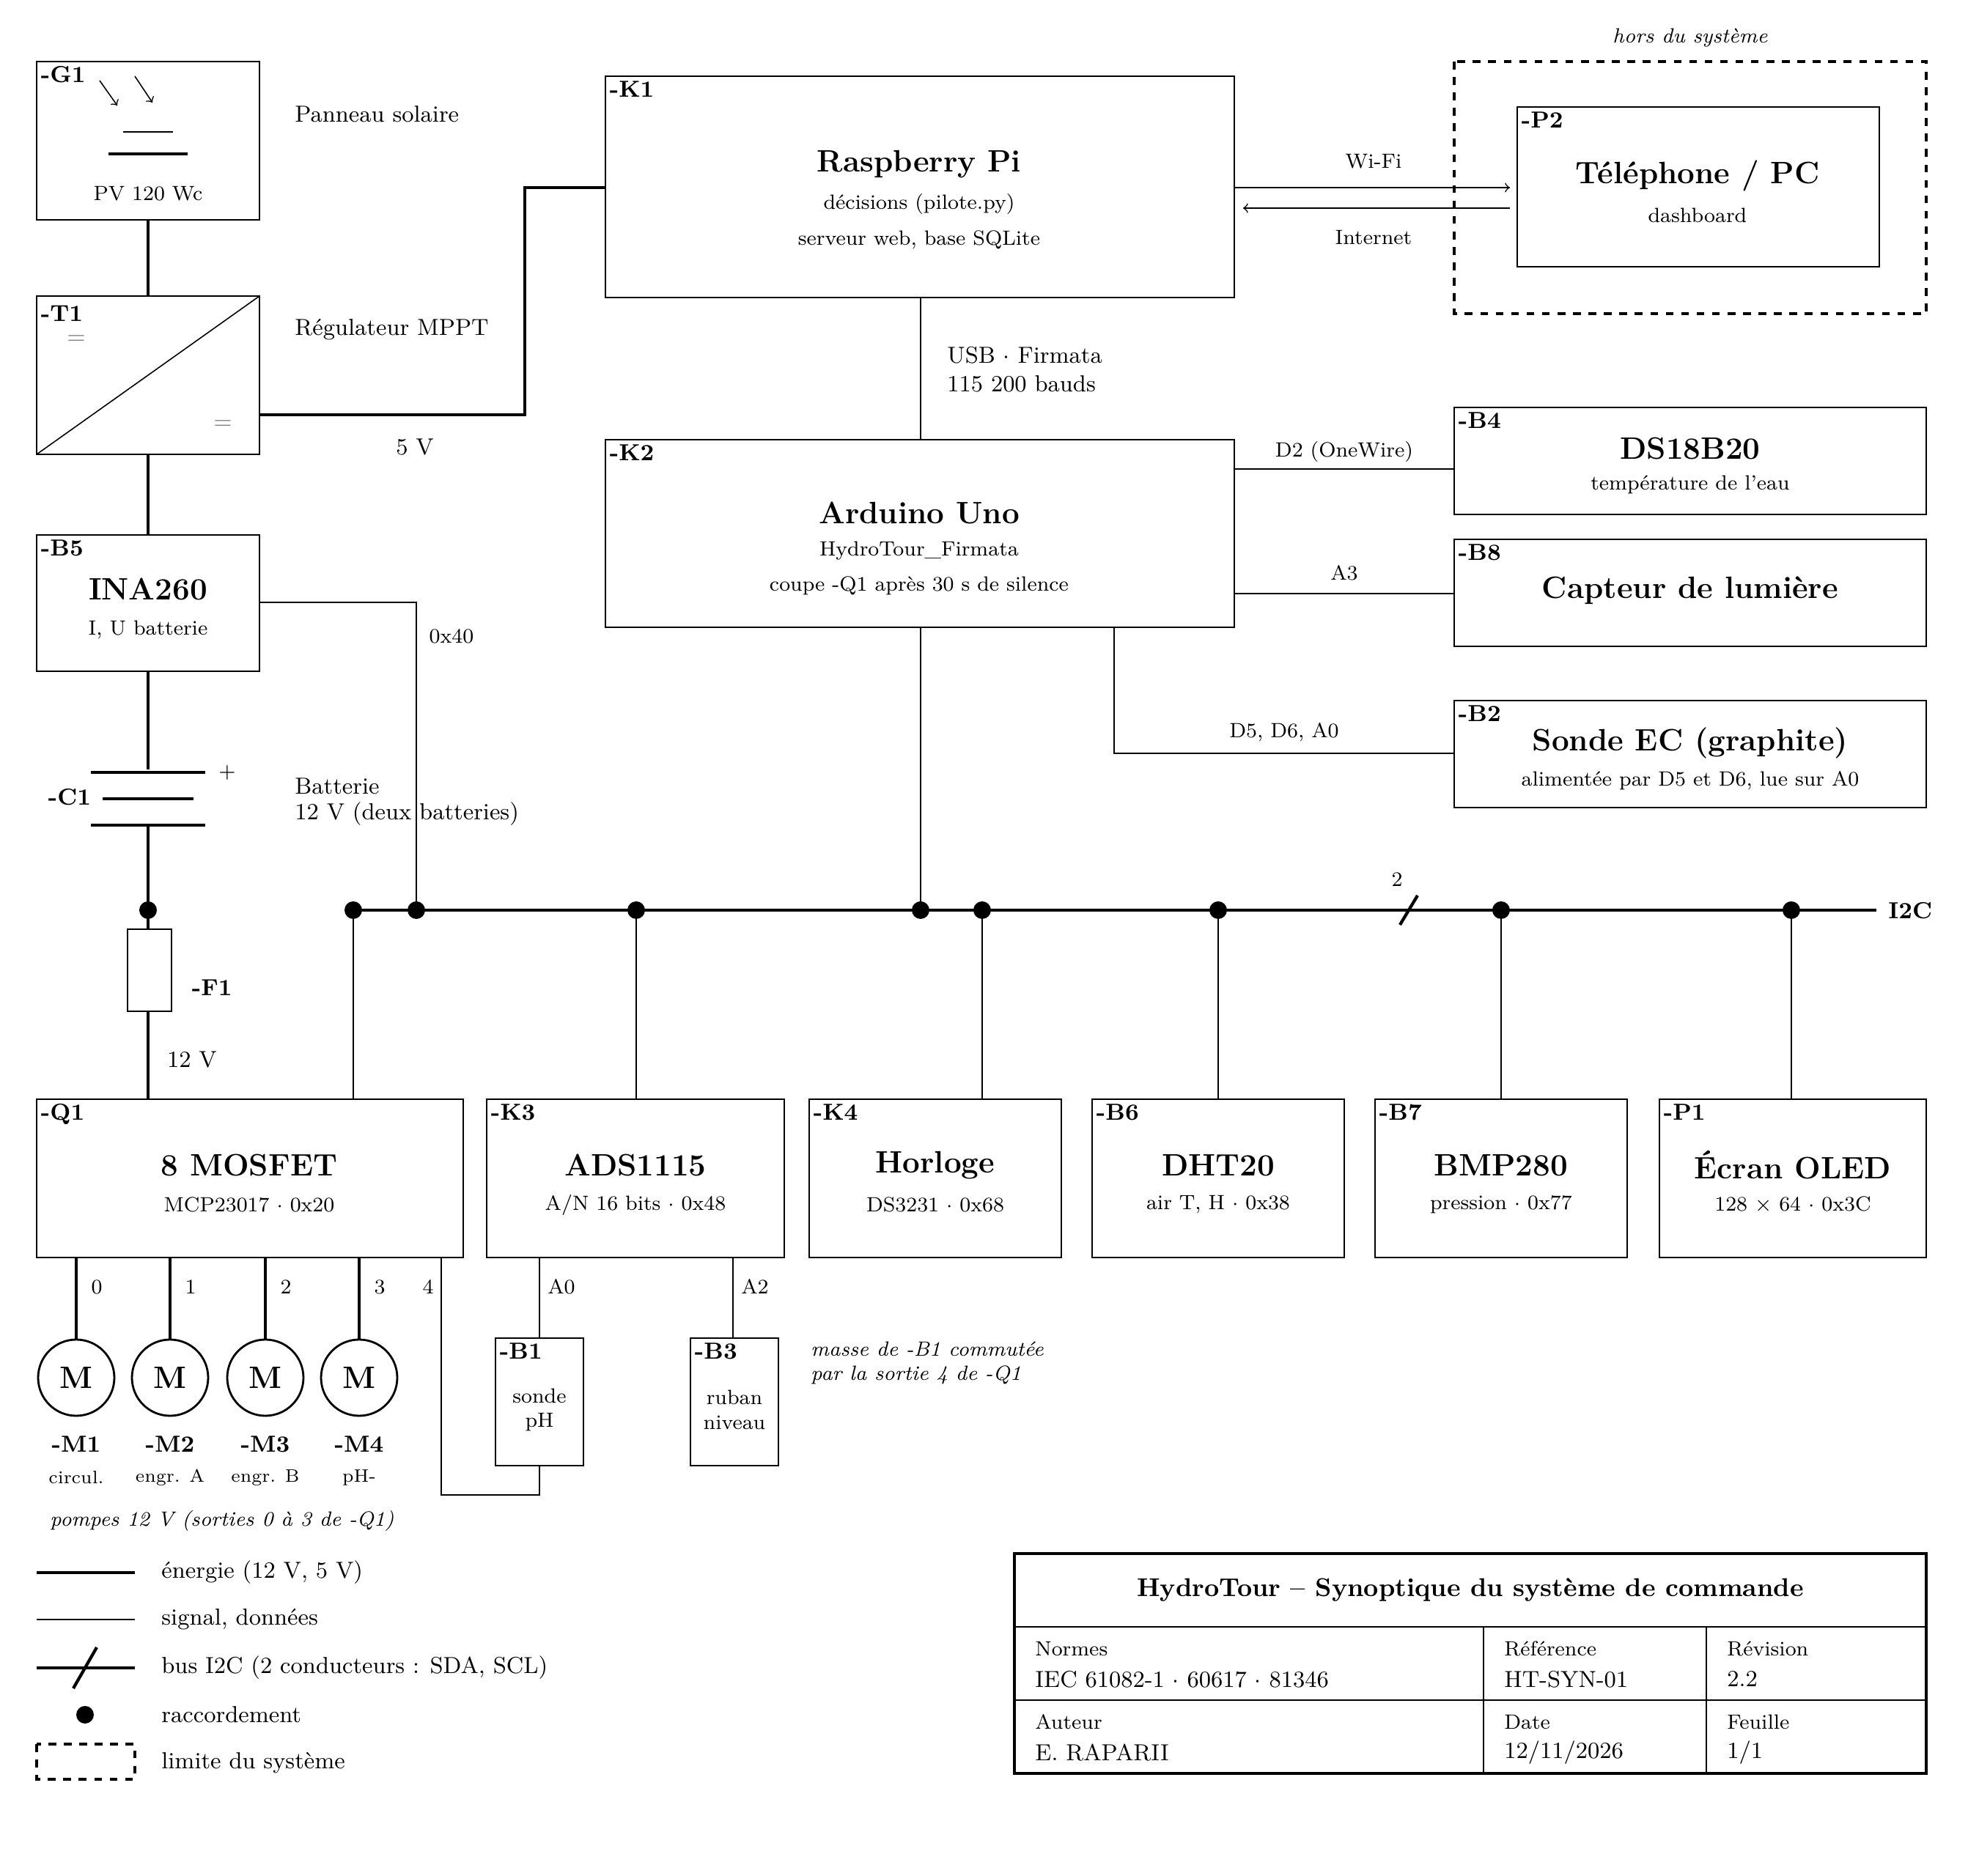
\includegraphics[width=\textwidth]{img/inf/f_synoptique.png}
\schemacap{synop}{Synoptique du système de commande (IEC 61082-1).}
\end{figure}

\schemapaysageC{eagle/schema_complet.pdf}{elcompl}{Schéma électrique complet de la tour (alimentation, commande, capteurs et sonde EC), sur une seule feuille.}


Le régulateur est un SLC-MT2024 : sa fiche (reproduite ci-dessous et dans l'Annexe 4) donne une tension d'entrée jusqu'à \qty{70}{V}, un courant de charge de \qty{20}{A}, une autoconsommation inférieure à \qty{15}{mA}, une charge en trois étages (absorption \qty{14,4}{V}, maintien \qty{13,8}{V}) et une coupure de charge à \qty{11,5}{V}. Ces réglages sont ceux d'une batterie au plomb. Mes batteries sont une Yuasa NP17-12I (\qty{17}{Ah}, plomb étanche) et une Steco YTX7A-BS (\qty{6}{Ah}, sans entretien, de type AGM). Le cahier des charges de départ parlait pourtant de batteries LiFePO4. Comme la technologie réelle se lit sur l'étiquette de chaque batterie, je calcule \textbf{les deux cas côte à côte} (LiFePO4 et plomb AGM) et je retiens le \textbf{plomb AGM} pour les conclusions de la tour, car c'est le cas défavorable et c'est celui des batteries que j'ai.

\schemapaysage[page=1]{SLC-MT2024.pdf}


\textbf{Conventions.} Les batteries sont des batteries de \qty{12}{V} nominal. Pour le LiFePO4, la tension moyenne en décharge vaut $U_B = \qty{12,8}{V}$ (4 éléments de \qty{3,2}{V}) ; pour le plomb AGM, $U_B = \qty{12,0}{V}$. Tous les courants côté \qty{12}{V} de la partie consommation sont calculés à \qty{12,8}{V} : à puissance égale, c'est le cas LiFePO4. Pour l'AGM, ces courants sont un peu plus forts, dans le rapport $12{,}8/12{,}0$, et les calculs correspondants sont donnés dans la partie 5.5.

\subsubsection*{Ce qui a changé depuis la version 1 de l'étude}

Cette version 2 reprend la structure, les données d'étiquette du panneau TE1250 et le rendement du convertisseur \qty{12}{V} vers \qty{5}{V} ($\eta = 0{,}83$) de la version 1. Les démonstrations sont réécrites et complétées. Le tableau résume les points qui changent.

\begin{table}[H]
\centering
\small
\begin{tabularx}{\textwidth}{|>{\raggedright\arraybackslash}p{2.6cm}|Y|Y|}
\hline
\textbf{Sujet} & \textbf{Version 1} & \textbf{Version 2} \\
\hline
Pompes & P1 à P5, dont une pompe d'appoint P5 et un bac de secours & Bac principal unique de \qty{152}{L}, appoint manuel. Pompes nommées par fonction : circulation, doseuses engrais A, engrais B, pH$-$ \\
\hline
Carte de puissance & Une sortie par pompe & Carte 6318 (8 MOSFET\ix{15}). Une sortie par pompe (circulation sur la sortie 0) \\
\hline
Capteurs & SHT31, BH1750, ADXL345, deux eTape\ix{23} & DHT, capteur de lumière analogique, LIS3DHTR (Sensor Kit), un seul eTape\ix{23}. pH sur l'entrée A1 de l'Arduino \\
\hline
Batteries & Plomb AGM supposé & LiFePO4 d'après le cahier des charges. Les deux cas sont calculés côte à côte (partie 5.5), la technologie réelle est à lire sur l'étiquette \\
\hline
Consommation & \qty{281}{Wh/j} & \qty{226,7}{Wh/j}. Écart surtout dû à l'électronique : \qty{91,8}{Wh/j} estimés composant par composant, contre \qty{149,8}{Wh/j} en version 1 (point d'essai du convertisseur à \qty{1}{A}). Pompe d'appoint retirée ; régulateur et MOSFET\ix{15} ajoutés. La mesure M2 tranchera \\
\hline
Production pire mois & \qty{336}{Wh/j} disponibles (avec $H = \qty{4,2}{kWh/m^2/j}$) & \qty{304,5}{Wh/j} (LiFePO4) ou \qty{272,4}{Wh/j} (AGM), avec $H = \qty{3,607}{kWh/m^2/j}$ en juin (Solargis) et des facteurs de pertes détaillés un par un \\
\hline
Fusibles & $F_{PV} = \qty{10}{A}$, $F_{B1} = \qty{5}{A}$, $F_{B2} = \qty{15}{A}$, $F_2 = \qty{7,5}{A}$ & $F_{PV}$, $F_{B1}$, $F_{B2}$ inchangés ; $F_2 = \qty{4}{A}$ (sans P5) ; nouveau $F_3 = \qty{2}{A}$ en entrée du convertisseur \qty{5}{V} \\
\hline
Calcul du panneau & Modèle à une diode, courbes du TE1250 à 25, 47, 50 et \qty{75}{\celsius} & Calcul direct sur le panneau entier, comparé aux mêmes courbes (écart inférieur à \qty{1}{\percent}) \\
\hline
Mesures & Absentes & Protocole complet, tableaux, fichiers modèles et script de traitement (partie 5.8) \\
\hline
\end{tabularx}
\caption{Ce qui change entre la version 1 et la version 2 de l'étude électrique.}
\end{table}

\begin{aretenir}
Sept fonctions : produire (panneau), réguler et protéger (MPPT\ix{19}, fusibles), stocker (batteries), mesurer l'énergie (INA260\ix{22}), convertir (UBEC\ix{17}), décider (Pi), lire et agir (Arduino, carte MOSFET\ix{15}, pompes, capteurs). Les deux technologies de batterie (LiFePO4 et plomb AGM) sont calculées ; l'AGM est retenu pour les conclusions.
\end{aretenir}

\Needspace{8\baselineskip}\subsection{Le schéma électrique}

Le schéma électrique complet est dessiné sur une seule feuille vectorielle (le zoom ne le floute pas), reproduite plus haut et en partie 8.1. Cette partie en donne la lecture et les règles de branchement.


\textbf{Lecture du schéma.} Les fils de puissance relient le panneau, le régulateur, les batteries, la carte MOSFET\ix{15} et le convertisseur. Les liaisons de données (bus I2C\ix{12}, signaux analogiques) sont dessinées à part. Chaque pompe se raccorde entre la borne $V+$ et la sortie MOSFET\ix{15} de son canal : la commutation se fait côté négatif, et la carte contient une diode de roue libre. La pompe de circulation est commandée par la sortie 0 de la carte (une sortie par pompe, partie 8.2). L'INA260\ix{22} est inséré entre la borne $BAT+$ du régulateur et le bus des batteries : il mesure le courant net (charge moins décharge) et la tension de la batterie. L'INA260\ix{22} est relié directement à l'Arduino (alimentation \qty{5}{V}, SDA\ix{13} et SCL\ix{14}) ; l'écran et les autres capteurs I2C\ix{12} sont sur un second bus de l'Arduino, qui leur fournit aussi le \qty{5}{V} et la masse ; le Raspberry Pi récupère la tension, le courant et le pourcentage de batterie auprès de l'Arduino. L'Arduino est alimenté en \qty{5}{V} et en données par l'USB du Raspberry Pi.



La notice du régulateur indique que c'est un contrôleur à positif commun : les bornes $PV+$, $BAT+$ et $LOAD+$ sont communes, et c'est le négatif qui est commuté. Les trois négatifs $PV-$, $BAT-$ et $LOAD-$ ne doivent donc jamais être reliés entre eux à l'extérieur. Chaque négatif va sur sa borne : le moins du panneau sur $PV-$, le moins des batteries sur $BAT-$, et la masse de la tour (carte MOSFET\ix{15}, UBEC\ix{17}, INA260\ix{22}) sur $LOAD-$.

\textbf{Ordre de branchement.} On branche d'abord les batteries, fusibles retirés jusqu'à la fin du câblage, puis le panneau. Le débranchement se fait dans l'ordre inverse. Cet ordre évite que le régulateur voie le panneau sans batterie, ce qui peut l'endommager.

\Needspace{8\baselineskip}\subsection{Le bilan de consommation}

\subsubsection*{Ce que je cherche et ce que je suppose}

Je cherche l'énergie $E_j$ consommée en une journée, en wattheures. Je la calcule composant par composant, en deux grands blocs : l'électronique alimentée en \qty{5}{V}, et ce qui est pris directement sur le \qty{12}{V} (pompes, pertes des MOSFET\ix{15}, autoconsommation du régulateur). Les courants de l'électronique sont des courants moyens en fonctionnement normal, estimés à partir des fiches techniques : ce sont des hypothèses, à vérifier par la mesure M2 (partie 5.8). La pompe de circulation de \qty{19}{W} tourne selon un planning, en heure de Tahiti : de 6 h à 18 h, \qty{15}{min} de marche puis \qty{15}{min} d'arrêt, soit 2 marches par heure pendant 12 h ; la nuit, \qty{15}{min} à 21 h, à 0 h et à 3 h.

\subsubsection*{L'électronique alimentée en 5 V}

Le Raspberry Pi, le dongle Wi-Fi, l'Arduino (par l'USB du Pi) et tous les capteurs sont alimentés en \qty{5}{V} par l'UBEC\ix{17}. Le tableau donne le courant moyen de chaque composant, sa puissance à \qty{5}{V} et son énergie sur 24 heures.

\begin{table}[H]
\centering
\small
\begin{tabularx}{\textwidth}{|>{\raggedright\arraybackslash}X|r|r|r|}
\hline
\textbf{Composant} & \textbf{$I$ moyen (mA)} & \textbf{$P$ à \qty{5}{V} (W)} & \textbf{$E$ sur \qty{24}{h} (Wh)} \\
\hline
Raspberry Pi 3 Model B (sans écran, charge faible) & 450 & 2,250 & 54,00 \\
\hline
Dongle Wi-Fi USB à antenne externe & 120 & 0,600 & 14,40 \\
\hline
Arduino Uno R3 & 50 & 0,250 & 6,00 \\
\hline
Base Grove (LED témoin) & 3 & 0,015 & 0,36 \\
\hline
Carte pH Gravity V2.0 & 5 & 0,025 & 0,60 \\
\hline
Sonde EC fabriquée (alimentée seulement à la lecture) & 0,2 & 0,001 & 0,02 \\
\hline
eTape\ix{23} \qty{30}{cm} et sa résistance de référence & 2 & 0,010 & 0,24 \\
\hline
ADS1115\ix{16} & 0,2 & 0,001 & 0,02 \\
\hline
DS18B20\ix{24} & 0,5 & 0,003 & 0,06 \\
\hline
Capteur d'humidité et de température de l'air & 0,3 & 0,002 & 0,04 \\
\hline
Capteur de lumière (analogique) & 0,5 & 0,003 & 0,06 \\
\hline
Accéléromètre LIS3DHTR & 0,02 & 0,000 & 0,00 \\
\hline
Module RTC (horloge) & 0,2 & 0,001 & 0,02 \\
\hline
INA260\ix{22} (partie logique) & 1,1 & 0,006 & 0,13 \\
\hline
Carte 6318 : MCP23017 et LED témoin & 2 & 0,010 & 0,24 \\
\hline
\textbf{Total côté \qty{5}{V}} & \textbf{635} & \textbf{3,175} & \textbf{76,20} \\
\hline
\end{tabularx}
\caption{Consommation moyenne de l'électronique alimentée en \qty{5}{V}.}
\end{table}

Le Raspberry Pi et le dongle Wi-Fi représentent à eux seuls \qty{90}{\percent} de la consommation de l'électronique : c'est là qu'une économie aurait un effet (désactiver le HDMI, les LED, le Bluetooth, le Wi-Fi interne si le dongle est utilisé).

\naturecalc{théorie (formule démontrée, valeurs de fiches techniques et hypothèses ; rien de mesuré)}
\begin{demonstration}[énergie consommée par un composant]
\resultat{E = P\,\Delta t}
Je note $P$ la puissance reçue par le composant, en watts, $U$ la tension à ses bornes, en volts, $I$ le courant qui le traverse, en ampères, $\Delta t$ la durée de fonctionnement, en heures, et $E$ l'énergie, en wattheures. La puissance instantanée reçue par un dipôle est le produit de la tension à ses bornes par le courant qui le traverse :
\begin{align*}
P &= U\, I
\end{align*}
L'énergie est l'intégrale de la puissance sur la durée $\Delta t$ :
\begin{align*}
E &= \int_{0}^{\Delta t} P(t)\,\mathrm{d}t
\end{align*}
Si $P$ est constante sur la durée de fonctionnement, elle sort de l'intégrale :
\begin{align*}
E &= P \int_{0}^{\Delta t} \mathrm{d}t\\
E &= P\,\Delta t
\end{align*}
Avec $P$ en watts et $\Delta t$ en heures, $E$ est en wattheures ($\qty{1}{Wh} = \qty{3600}{J}$). Pour un courant \emph{moyen} $\bar I$ sous tension constante, $\bar P = U \bar I$ donne la même énergie que le courant réel.
\end{demonstration}

\naturecalc{théorie (formule démontrée, valeurs de fiches techniques et hypothèses ; rien de mesuré)}
\begin{demonstration}[énergie de l'électronique alimentée en 5 V]
\resultat{E_5 = \qty{76,2}{Wh/j}}
Tous les composants sont en parallèle sur le \qty{5}{V} : leurs courants s'additionnent. Le courant total côté \qty{5}{V}, en ampères, vaut (somme de la colonne du tableau) :
\begin{align*}
I_5 &= \qty{0,635}{A}
\end{align*}
La puissance côté \qty{5}{V}, en watts, vaut :
\begin{align*}
P_5 &= U_5\, I_5\\
P_5 &= \qty{5,0}{V} \times \qty{0,635}{A}\\
P_5 &= \qty{3,175}{W}
\end{align*}
L'énergie sur une journée de \qty{24}{h} vaut :
\begin{align*}
E_5 &= P_5\,\Delta t\\
E_5 &= \qty{3,175}{W} \times \qty{24}{h}\\
E_5 &= \qty{76,2}{Wh/j}
\end{align*}
\end{demonstration}

\subsubsection*{Les pertes du convertisseur 12 V vers 5 V}

L'UBEC\ix{17} n'est pas parfait : il prend sur le \qty{12}{V} plus de puissance qu'il n'en rend sur le \qty{5}{V}, et la différence part en chaleur.

\naturecalc{théorie (formule démontrée, valeurs de fiches techniques et hypothèses ; rien de mesuré)}
\begin{demonstration}[puissance absorbée par un convertisseur]
\resultat{P_{entrée} = \dfrac{P_{sortie}}{\eta}}
Je note $\eta$ le rendement du convertisseur (sans unité), $P_{sortie}$ la puissance utile fournie, en watts, et $P_{entrée}$ la puissance absorbée, en watts. Le rendement est le rapport de la puissance utile fournie à la puissance absorbée :
\begin{align*}
\eta &= \frac{P_{sortie}}{P_{entrée}}
\end{align*}
J'isole la puissance d'entrée :
\begin{align*}
P_{entrée} &= \frac{P_{sortie}}{\eta}
\end{align*}
La puissance perdue (chaleur) est la différence, puis je factorise $P_{sortie}$ :
\begin{align*}
P_{pertes} &= P_{entrée} - P_{sortie}\\
P_{pertes} &= \frac{P_{sortie}}{\eta} - P_{sortie}\\
P_{pertes} &= P_{sortie}\left(\frac{1}{\eta} - 1\right)
\end{align*}
\end{demonstration}

\naturecalc{théorie (formule démontrée, valeurs de fiches techniques et hypothèses ; rien de mesuré)}
\begin{demonstration}[puissance prise sur le 12 V par l'électronique]
\resultat{E_{12,e} = \qty{91,8}{Wh/j}}
Je prends $\eta = 0{,}83$ (valeur de la version 1, à confirmer par la mesure M2) et $P_{sortie} = P_5 = \qty{3,175}{W}$. La puissance prise sur le \qty{12}{V} vaut :
\begin{align*}
P_{12,e} &= \frac{P_5}{\eta}\\
P_{12,e} &= \frac{\qty{3,175}{W}}{0{,}83}\\
P_{12,e} &\approx \qty{3,825}{W}
\end{align*}
La puissance perdue dans le convertisseur vaut :
\begin{align*}
P_{conv} &= P_5\left(\frac{1}{\eta} - 1\right)\\
P_{conv} &= \qty{3,175}{W} \times \left(\frac{1}{0{,}83} - 1\right)\\
P_{conv} &\approx \qty{0,650}{W}
\end{align*}
Le courant moyen pris sur la batterie par l'électronique, sous $U_B = \qty{12,8}{V}$, vaut :
\begin{align*}
I_{12,e} &= \frac{P_{12,e}}{U_B}\\
I_{12,e} &= \frac{\qty{3,825}{W}}{\qty{12,8}{V}}\\
I_{12,e} &\approx \qty{0,299}{A}
\end{align*}
L'énergie journalière prise sur le \qty{12}{V} vaut (dont $\qty{0,650}{W} \times \qty{24}{h} = \qty{15,6}{Wh}$ de pertes) :
\begin{align*}
E_{12,e} &= P_{12,e} \times \Delta t\\
E_{12,e} &= \qty{3,825}{W} \times \qty{24}{h}\\
E_{12,e} &\approx \qty{91,8}{Wh/j}
\end{align*}
\end{demonstration}

\subsubsection*{La pompe de circulation}

\naturecalc{théorie (formule démontrée, valeurs de fiches techniques et hypothèses ; rien de mesuré)}
\begin{demonstration}[durée de marche journalière et énergie de la pompe]
\resultat{t_c = \qty{6,75}{h/j} \quad\text{et}\quad E_c = \qty{128,25}{Wh/j}}
Je note $t_c$ la durée de marche par jour, en heures. De jour, il y a 12 heures et 2 marches de \qty{0,25}{h} par heure :
\begin{align*}
t_{jour} &= 12 \times 2 \times \qty{0,25}{h}\\
t_{jour} &= \qty{6,00}{h}
\end{align*}
De nuit (de 18 h à 6 h), il y a 3 marches de \qty{0,25}{h}, à 21 h, 0 h et 3 h :
\begin{align*}
t_{nuit} &= 3 \times \qty{0,25}{h}\\
t_{nuit} &= \qty{0,75}{h}
\end{align*}
\begin{align*}
t_c &= \qty{6,00}{h} + \qty{0,75}{h}\\
t_c &= \qty{6,75}{h/j}
\end{align*}
Avec la puissance $P_c = \qty{19}{W}$ de la pompe LPFIDI (donnée de la fiche), l'énergie d'après la démonstration précédente vaut :
\begin{align*}
E_c &= P_c\, t_c\\
E_c &= \qty{19}{W} \times \qty{6,75}{h/j}\\
E_c &= \qty{128,25}{Wh/j}
\end{align*}
Le courant de la pompe sous $U_B = \qty{12,8}{V}$ vaut :
\begin{align*}
I_c &= \frac{P_c}{U_B}\\
I_c &= \frac{\qty{19}{W}}{\qty{12,8}{V}}\\
I_c &\approx \qty{1,48}{A}
\end{align*}
\end{demonstration}

\subsubsection*{Les pertes dans les MOSFET de la carte 6318}

Chaque canal de la carte utilise un transistor MOSFET\ix{15} dont la résistance à l'état passant vaut $R_{DS(on)} = \qty{70}{m\ohm}$ (valeur de fiche du composant). La pompe de circulation est branchée sur un seul canal (sortie 0).

\naturecalc{théorie (formule démontrée, valeurs de fiches techniques et hypothèses ; rien de mesuré)}
\begin{demonstration}[pertes MOSFET\ix{15} de la circulation]
\resultat{E_{MOS} \approx \qty{1,04}{Wh/j}}
Je note $I$ le courant de la pompe, en ampères, et $U_{DS}$ la tension aux bornes du MOSFET\ix{15}, en volts. Un MOSFET\ix{15} saturé se comporte comme une résistance $R_{DS(on)}$. La loi d'Ohm donne $U_{DS} = R_{DS(on)}\, I$, donc la puissance dissipée, en watts, vaut :
\begin{align*}
P_1 &= U_{DS}\, I\\
P_1 &= R_{DS(on)}\, I^2
\end{align*}
Avec $I = I_c = \qty{1,48}{A}$ :
\begin{align*}
P_1 &= \qty{0,070}{\ohm} \times (\qty{1,48}{A})^2\\
P_1 &\approx \qty{0,154}{W}
\end{align*}
L'énergie perdue par jour, pendant $t_c = \qty{6,75}{h}$, vaut :
\begin{align*}
E_{MOS} &= P_1\, t_c\\
E_{MOS} &= \qty{0,154}{W} \times \qty{6,75}{h}\\
E_{MOS} &\approx \qty{1,04}{Wh/j}
\end{align*}
\end{demonstration}

\subsubsection*{Les pompes doseuses}

Les trois pompes péristaltiques\ix{8} (engrais A, engrais B, pH$-$) absorbent environ $I_d = \qty{0,30}{A}$ sous \qty{12}{V} et débitent environ $Q = \qty{80}{mL/min}$ en charge (hypothèse, à mesurer : mesure M5). Leur puissance sous $U_B = \qty{12,8}{V}$ vaut :
\begin{align*}
P_d &= U_B\, I_d\\
P_d &= \qty{12,8}{V} \times \qty{0,30}{A}\\
P_d &= \qty{3,84}{W}
\end{align*}

Pour estimer le volume d'engrais dosé par jour, je pars du fait que les laitues prélèvent les sels minéraux, donc que l'EC baisse. Je suppose une baisse de $\Delta EC = \qty{0,05}{mS/cm}$ par jour dans le bac de $V_{bac} = \qty{152}{L}$, et une solution mère telle qu'ajouter \qty{1}{mL} de A et \qty{1}{mL} de B par litre d'eau augmente l'EC de $s = \qty{0,56}{mS/cm}$ (hypothèses à confirmer par l'étude hydraulique et chimique).

\naturecalc{théorie (formule démontrée, valeurs de fiches techniques et hypothèses ; rien de mesuré)}
\begin{demonstration}[volume de solution mère pour corriger l'EC]
\resultat{V_A = \dfrac{\Delta EC\; V_{bac}}{s} \approx \qty{13,6}{mL/j}}
Je note $d$ la dose de solution mère par litre de bac, en mL/L, $V_A$ le volume ajouté, en mL, et $Q$ le débit de la pompe, en mL/min. En solution diluée, l'EC est proportionnelle à la concentration en sels, donc à la dose :
\begin{align*}
\Delta EC &= s\, d
\end{align*}
La dose est le volume ajouté divisé par le volume du bac :
\begin{align*}
d &= \frac{V_A}{V_{bac}}
\end{align*}
Je remplace et j'isole $V_A$ :
\begin{align*}
\Delta EC &= s\,\frac{V_A}{V_{bac}}\\
V_A &= \frac{\Delta EC\; V_{bac}}{s}
\end{align*}
La durée de fonctionnement d'une pompe de débit $Q$ est le volume divisé par le débit :
\begin{align*}
t &= \frac{V}{Q}
\end{align*}
Application, avec $s = \qty{0,56}{(mS/cm)/(mL/L)}$ :
\begin{align*}
V_A &= \frac{\qty{0,05}{mS/cm} \times \qty{152}{L}}{\qty{0,56}{(mS/cm)/(mL/L)}}\\
V_A &\approx \qty{13,6}{mL/j}
\end{align*}
Le même volume d'engrais B est dosé : $V_B = \qty{13,6}{mL/j}$. Pour le pH$-$, je suppose $V_{pH} = \qty{6}{mL/j}$. Les durées de marche valent :
\begin{align*}
t_A &= \frac{\qty{13,6}{mL}}{\qty{80}{mL/min}} = \qty{0,170}{min} = \qty{10,2}{s}\\
t_B &= \qty{10,2}{s}\\
t_{pH} &= \frac{\qty{6}{mL}}{\qty{80}{mL/min}} = \qty{0,075}{min} = \qty{4,5}{s}
\end{align*}
L'énergie estimée vaut :
\begin{align*}
E_{d,est} &= \qty{3,84}{W} \times \frac{(10{,}2 + 10{,}2 + 4{,}5)\,\unit{s}}{\qty{3600}{s/h}}\\
E_{d,est} &\approx \qty{0,027}{Wh/j}
\end{align*}
Valeur retenue (majorant) : le programme limite chaque commande à \qty{30}{s}. Je suppose au plus 10 commandes de \qty{30}{s} par pompe et par jour (cas d'un dérèglement) :
\begin{align*}
E_d &= 3 \times 10 \times \qty{30}{s} \times \frac{\qty{3,84}{W}}{\qty{3600}{s/h}}\\
E_d &= \qty{0,96}{Wh/j}
\end{align*}
\end{demonstration}

\subsubsection*{L'autoconsommation du régulateur}

\naturecalc{théorie (formule démontrée, valeurs de fiches techniques et hypothèses ; rien de mesuré)}
\begin{demonstration}[autoconsommation du régulateur MPPT\ix{19}]
\resultat{E_{MPPT\ix{19}} \approx \qty{4,61}{Wh/j}}
Le régulateur consomme un courant propre $I_{MPPT} = \qty{15}{mA}$ (valeur de la fiche), jour et nuit, sous $U_B = \qty{12,8}{V}$ :
\begin{align*}
P_{MPPT} &= U_B\, I_{MPPT}\\
P_{MPPT} &= \qty{12,8}{V} \times \qty{0,015}{A}\\
P_{MPPT} &= \qty{0,192}{W}
\end{align*}
\begin{align*}
E_{MPPT} &= P_{MPPT} \times \qty{24}{h}\\
E_{MPPT} &= \qty{0,192}{W} \times \qty{24}{h}\\
E_{MPPT} &\approx \qty{4,61}{Wh/j}
\end{align*}
\end{demonstration}

\subsubsection*{L'énergie journalière totale}

Le tableau suivant additionne les consommations de chaque élément pour donner le bilan journalier de la tour.

\begin{table}[H]
\centering
\small
\begin{tabular}{|l|r|r|r|}
\hline
\textbf{Poste} & \textbf{$P$ (W)} & \textbf{Durée (h/j)} & \textbf{$E$ (Wh/j)} \\
\hline
Électronique \qty{5}{V} (vue du \qty{12}{V}, pertes UBEC\ix{17} comprises) & 3,825 & 24 & 91,81 \\
\hline
\quad dont pertes du convertisseur & 0,650 & 24 & 15,61 \\
\hline
Pompe de circulation & 19,0 & 6,75 & 128,25 \\
\hline
Pertes MOSFET\ix{15} circulation (un canal) & 0,154 & 6,75 & 1,04 \\
\hline
Pompes doseuses (majorant) & 3,84 & 0,25 & 0,96 \\
\hline
Autoconsommation du MPPT\ix{19} & 0,192 & 24 & 4,61 \\
\hline
\textbf{Total} & & & \textbf{226,7} \\
\hline
\end{tabular}
\caption{Bilan de consommation journalière de la tour.}
\end{table}

\naturecalc{théorie (formule démontrée, valeurs de fiches techniques et hypothèses ; rien de mesuré)}
\begin{demonstration}[énergie journalière totale]
\resultat{E_j \approx \qty{226,7}{Wh/j}}
Je somme tous les postes (ceux du tableau, hors la ligne « dont pertes », déjà comptée dans l'électronique) :
\begin{align*}
E_j &= E_{12,e} + E_c + E_{MOS} + E_d + E_{MPPT}\\
E_j &= \qty{91,81}{Wh/j} + \qty{128,25}{Wh/j} + \qty{1,04}{Wh/j} + \qty{0,96}{Wh/j} + \qty{4,61}{Wh/j}\\
E_j &= \qty{226,67}{Wh/j}\\
E_j &\approx \qty{226,7}{Wh/j}
\end{align*}
La pompe de circulation pèse $\qty{128,25}{Wh/j}/\qty{226,7}{Wh/j} \approx 57\,\%$ du total, l'électronique $\qty{91,8}{Wh/j}/\qty{226,7}{Wh/j} \approx 40\,\%$.
\end{demonstration}

La figure suivante montre la part de chaque élément dans la consommation journalière de \qty{227}{Wh/j}.

\begin{figure}[H]
\centering
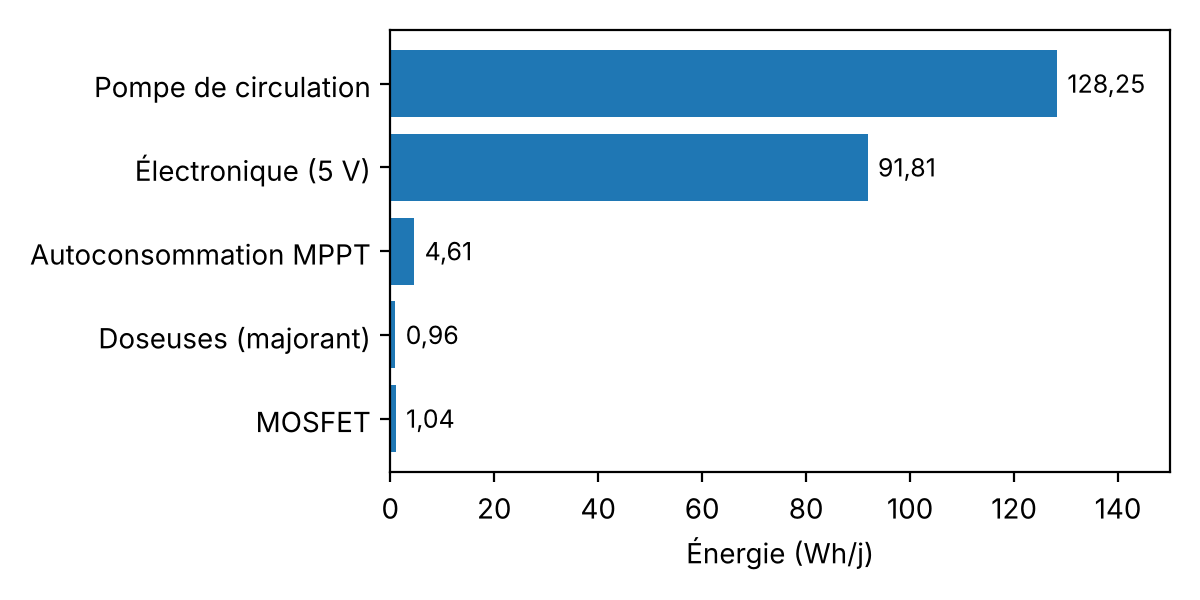
\includegraphics[width=0.78\textwidth]{img/conso.png}
\caption{Répartition de la consommation journalière : \qty{227}{Wh/j} au total.}
\end{figure}

\begin{aretenir}
Besoin journalier : $E_j = \qty{226,7}{Wh/j}$ (version 1 : \qty{281}{Wh/j}). Circulation \qty{128,25}{Wh} (57\,\%), électronique \qty{91,8}{Wh} (40\,\%) dont \qty{15,6}{Wh} de pertes du convertisseur, doseuses moins de \qty{1}{Wh}. Courant de repos sur le \qty{12}{V} : environ \qty{0,31}{A} ; courant de la pompe de circulation : \qty{1,48}{A}. Les pertes du MOSFET\ix{15} (un seul canal) valent \qty{0,154}{W}, soit \qty{1,04}{Wh/j}. La seule économie sérieuse possible est de réduire le temps de marche de la pompe ou la consommation du Raspberry Pi.
\end{aretenir}


\tcbset{enobox/.append style={unbreakable}}
\Needspace{8\baselineskip}\subsection{Le dimensionnement du panneau}

\subsubsection*{Ce que je cherche et ce que je suppose}

Je pars de l'hypothèse que je n'ai pas encore de panneau. Je connais le besoin de la tour : $E_j = \qty{226,7}{Wh/j}$ (partie 5.3). Je cherche la puissance crête $P_c$, en watts-crête, qu'il faut pour couvrir ce besoin pendant le pire mois, puis je vérifie que le panneau que j'ai, le TE1250 de \qty{120}{Wc}, convient. Il me faut pour cela trois choses : l'énergie que le soleil apporte à Moorea pendant le pire mois, la part de cette énergie qui arrive vraiment dans les batteries (les pertes), et la formule qui relie ces grandeurs à la puissance crête. Je commence par l'ensoleillement.

\subsubsection*{L'ensoleillement à Moorea et le pire mois}

Pour l'ensoleillement, je prends les données de Solargis publiées par la Banque mondiale, moyennées sur les années 1999 à 2018. La grandeur utile est l'irradiation globale horizontale, notée GHI : c'est l'énergie solaire reçue par un mètre carré horizontal, en kWh/m$^2$. Les cartes ci-dessous donnent sa moyenne par jour, et le potentiel de production d'un panneau (PVOUT). Moorea est entourée en rouge.

\begin{figure}[H]
\centering
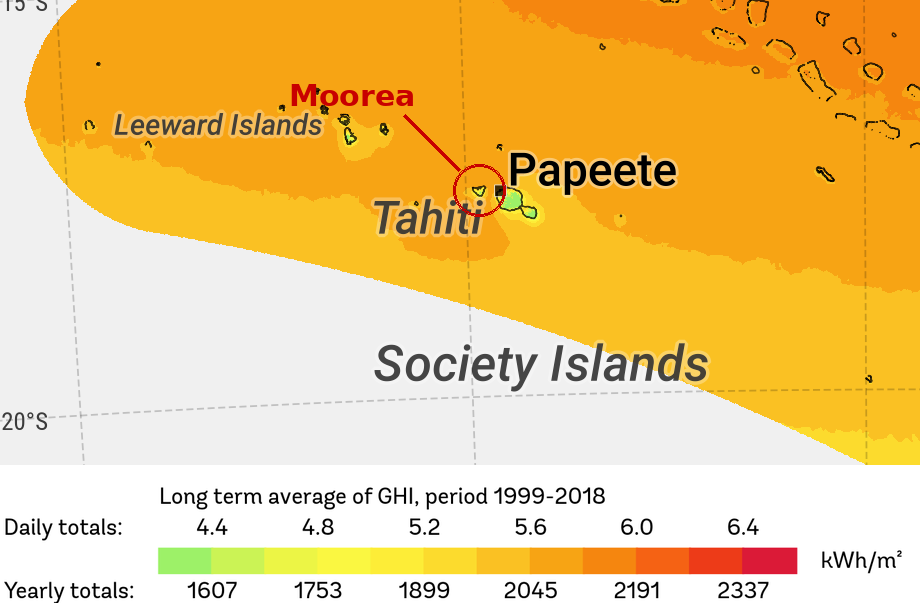
\includegraphics[width=0.86\textwidth]{img/solargis_ghi.png}
\caption{Irradiation globale horizontale (GHI), moyenne journalière sur 1999 à 2018, en Polynésie française (zone des îles de la Société). \copyright\ 2019 The World Bank, source : Global Solar Atlas 2.0, données Solargis. Le cercle rouge et le nom de Moorea ont été ajoutés.}
\end{figure}

Sur cette carte, les points de Moorea se répartissent entre les tranches de \num{4,4} à \qty{5,2}{kWh/m^2/j}, plus bas que l'océan autour (plus de \qty{5,4}{kWh/m^2/j}). Une carte ne donne qu'une moyenne sur l'année : elle ne dit pas quel mois est le plus sombre. Pour cela, je prends les moyennes mensuelles du Global Solar Atlas, qui repose sur les mêmes données Solargis, au point de Moorea (\qty{17,54}{\degree} sud, \qty{149,83}{\degree} ouest). Ces valeurs sont à valider avec mon tuteur.

\begin{figure}[H]
\centering
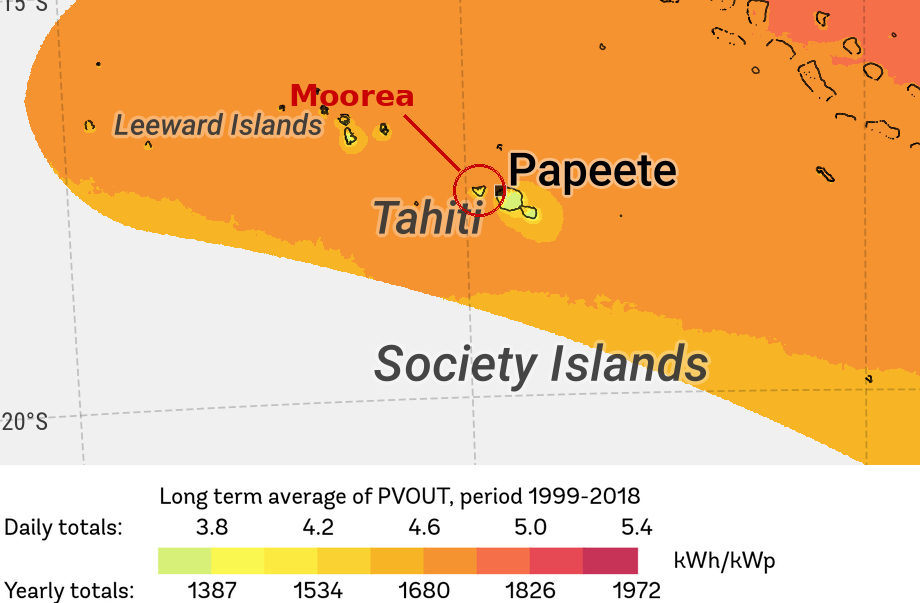
\includegraphics[width=0.86\textwidth]{img/solargis_pvout.png}
\caption{Potentiel de production photovoltaïque (PVOUT), moyenne journalière sur 1999 à 2018, en kWh par kWc. \copyright\ 2019 The World Bank, source : Global Solar Atlas 2.0, données Solargis. Le cercle rouge et le nom de Moorea ont été ajoutés.}
\end{figure}

La carte du PVOUT sert seulement de contrôle : elle suppose un panneau incliné de façon optimale et ses propres pertes, alors que je détaille moi-même chaque perte plus bas. Je ne m'en sers donc pas pour le calcul.

\naturecalc[22]{théorie (formule démontrée) appliquée à des données de Solargis ; rien de mesuré}
\begin{demonstration}[le pire mois d'ensoleillement]
\resultat{H_{pire} = \dfrac{G_{juin}}{N_{juin}} = \dfrac{\qty{108,21}{kWh/m^2}}{\qty{30}{j}} \approx \qty{3,607}{kWh/m^2/j}}
Je note $G_m$ l'irradiation reçue pendant le mois $m$, en kWh/m$^2$ par mois (donnée de Solargis), $N_m$ le nombre de jours de ce mois, et $H_m$ l'irradiation journalière moyenne du mois, en kWh/m$^2$/j. Le mois reçoit $G_m$ répartie sur $N_m$ jours, donc :
\begin{align*}
H_m &= \frac{G_m}{N_m}
\end{align*}
Le pire mois est celui où $H_m$ est le plus petit. Je calcule $H_m$ pour les douze mois dans le tableau ; le plus petit est juin :
\begin{align*}
H_{juin} &= \frac{\qty{108,21}{kWh/m^2}}{\qty{30}{j}}\\
H_{juin} &\approx \qty{3,607}{kWh/m^2/j}
\end{align*}
La moyenne sur l'année vaut $\qty{1731,45}{kWh/m^2}/\qty{365}{j} \approx \qty{4,74}{kWh/m^2/j}$ : le pire mois reçoit environ $\num{3,607}/\num{4,74} \approx 76\,\%$ de la moyenne.
\end{demonstration}

\begin{table}[H]
\centering
\small
\begin{tabular}{|l|c|c|c|}
\hline
\textbf{Mois} & \textbf{$G_m$ (kWh/m$^2$/mois)} & \textbf{$N_m$ (j)} & \textbf{$H_m$ (kWh/m$^2$/j)} \\
\hline
Janvier & 167,06 & 31 & 5,39 \\
\hline
Février & 153,28 & 28 & 5,47 \\
\hline
Mars & 164,42 & 31 & 5,30 \\
\hline
Avril & 136,11 & 30 & 4,54 \\
\hline
Mai & 122,48 & 31 & 3,95 \\
\hline
\textbf{Juin} & \textbf{108,21} & \textbf{30} & \textbf{3,61} \\
\hline
Juillet & 116,90 & 31 & 3,77 \\
\hline
Août & 134,17 & 31 & 4,33 \\
\hline
Septembre & 143,79 & 30 & 4,79 \\
\hline
Octobre & 158,01 & 31 & 5,10 \\
\hline
Novembre & 160,17 & 30 & 5,34 \\
\hline
Décembre & 166,84 & 31 & 5,38 \\
\hline
\end{tabular}
\caption{Irradiation globale horizontale à Moorea, moyennes 1999 à 2018 (Global Solar Atlas, données Solargis). La pire période est mai à juillet, et le pire mois est juin.}
\end{table}

La pire période est l'hiver austral, de mai à juillet, et le pire mois est juin. Le même site donne aussi l'irradiation sur un plan incliné de \qty{17}{\degree}, l'inclinaison optimale : \qty{129,24}{kWh/m^2} en juin, soit \qty{4,31}{kWh/m^2/j} ou \qty{19}{\percent} de plus que le plan horizontal. Mon panneau est incliné, mais son angle n'est pas fixé : je prends donc le plan horizontal pour dimensionner, et ce gain éventuel reste une marge en plus.

\subsubsection*{Le panneau que j'ai et ses données}

Je pars des données de l'étiquette du TE1250, dans les conditions standard (STC : \qty{1000}{W/m^2} et \qty{25}{\celsius}).

\begin{table}[H]
\centering
\small
\begin{tabular}{|l|c|c|}
\hline
\textbf{Grandeur (conditions STC)} & \textbf{Symbole} & \textbf{Valeur} \\
\hline
Puissance crête & $P_c$ & \qty{120}{Wc} \\
\hline
Puissance minimale garantie & $P_{\min}$ & \qty{117,5}{W} \\
\hline
Tension au point de puissance maximale & $V_{mp}$ & \qty{17,6}{V} \\
\hline
Courant au point de puissance maximale & $I_{mp}$ & \qty{6,8}{A} \\
\hline
Courant de court-circuit & $I_{sc}$ & \qty{7,3}{A} \\
\hline
Tension de circuit ouvert & $V_{oc}$ & \qty{22,0}{V} \\
\hline
Calibre maximal du fusible série & & \qty{10}{A} \\
\hline
\end{tabular}
\caption{Données d'étiquette du TE1250.}
\end{table}

Les coefficients de température du TE1250 ne figurent pas sur l'étiquette : je prends ceux du SLP055 (même technologie, 36 cellules), soit $\beta_V = -\qty{80}{mV/\celsius}$ pour la tension, $\gamma_P = -\qty{0,5}{\percent/\celsius}$ pour la puissance et une NOCT de \qty{47}{\celsius}. Je suppose une température d'air de \qty{27}{\celsius} en milieu de journée du pire mois (hypothèse).

\Needspace{30\baselineskip}\subsubsection*{La température des cellules}

\naturecalc[26]{théorie (formule démontrée, valeurs de fiches techniques et hypothèses ; rien de mesuré)}
\begin{demonstration}[température de cellule à partir de la NOCT]
\resultat{T_c = T_a + \dfrac{\mathrm{NOCT} - \qty{20}{\celsius}}{\qty{800}{W/m^2}}\, G \approx \qty{54}{\celsius}}
Je note $T_a$ la température de l'air, en °C, $T_c$ celle de la cellule, en °C, $G$ l'éclairement, en W/m$^2$, $\alpha$ la part de la lumière absorbée (sans unité) et $h$ le coefficient d'échange avec l'air, en W/(m$^2\cdot$K). La cellule reçoit une puissance proportionnelle à l'éclairement et la cède à l'air par convection et rayonnement, de façon à peu près proportionnelle à l'écart de température. En régime établi, puissance reçue égale puissance cédée :
\begin{align*}
\alpha\, G &= h\,(T_c - T_a)\\
T_c - T_a &= \frac{\alpha}{h}\, G = K\, G
\end{align*}
La NOCT est la température atteinte sous $G = \qty{800}{W/m^2}$ avec $T_a = \qty{20}{\celsius}$ (donnée de la fiche : \qty{47}{\celsius}) :
\begin{align*}
\mathrm{NOCT} - \qty{20}{\celsius} &= K \times \qty{800}{W/m^2}\\
K &= \frac{\mathrm{NOCT} - \qty{20}{\celsius}}{\qty{800}{W/m^2}}\\
T_c &= T_a + \frac{\mathrm{NOCT} - \qty{20}{\celsius}}{\qty{800}{W/m^2}}\, G
\end{align*}
Application, avec $T_a = \qty{27}{\celsius}$ et $G = \qty{800}{W/m^2}$ en milieu de journée du pire mois :
\begin{align*}
T_c &= \qty{27}{\celsius} + \frac{\qty{47}{\celsius} - \qty{20}{\celsius}}{\qty{800}{W/m^2}} \times \qty{800}{W/m^2}\\
T_c &= \qty{27}{\celsius} + \qty{27}{\celsius}\\
T_c &= \qty{54}{\celsius}
\end{align*}
\end{demonstration}

\Needspace{12\baselineskip}\subsubsection*{La puissance du panneau selon la température}

Je calcule directement sur le panneau entier, sans passer par un modèle de cellule. La figure donne les caractéristiques courant-tension et puissance-tension du TE1250, reprises de mon étude électrique de départ, sous \qty{1000}{W/m^2}, à quatre températures de cellule. Les températures de \qty{25}{\celsius} (conditions standard), \qty{47}{\celsius} (NOCT) et \qty{75}{\celsius} (cas extrême) encadrent la température de \qty{54}{\celsius} calculée plus haut.

\begin{figure}[H]
\centering
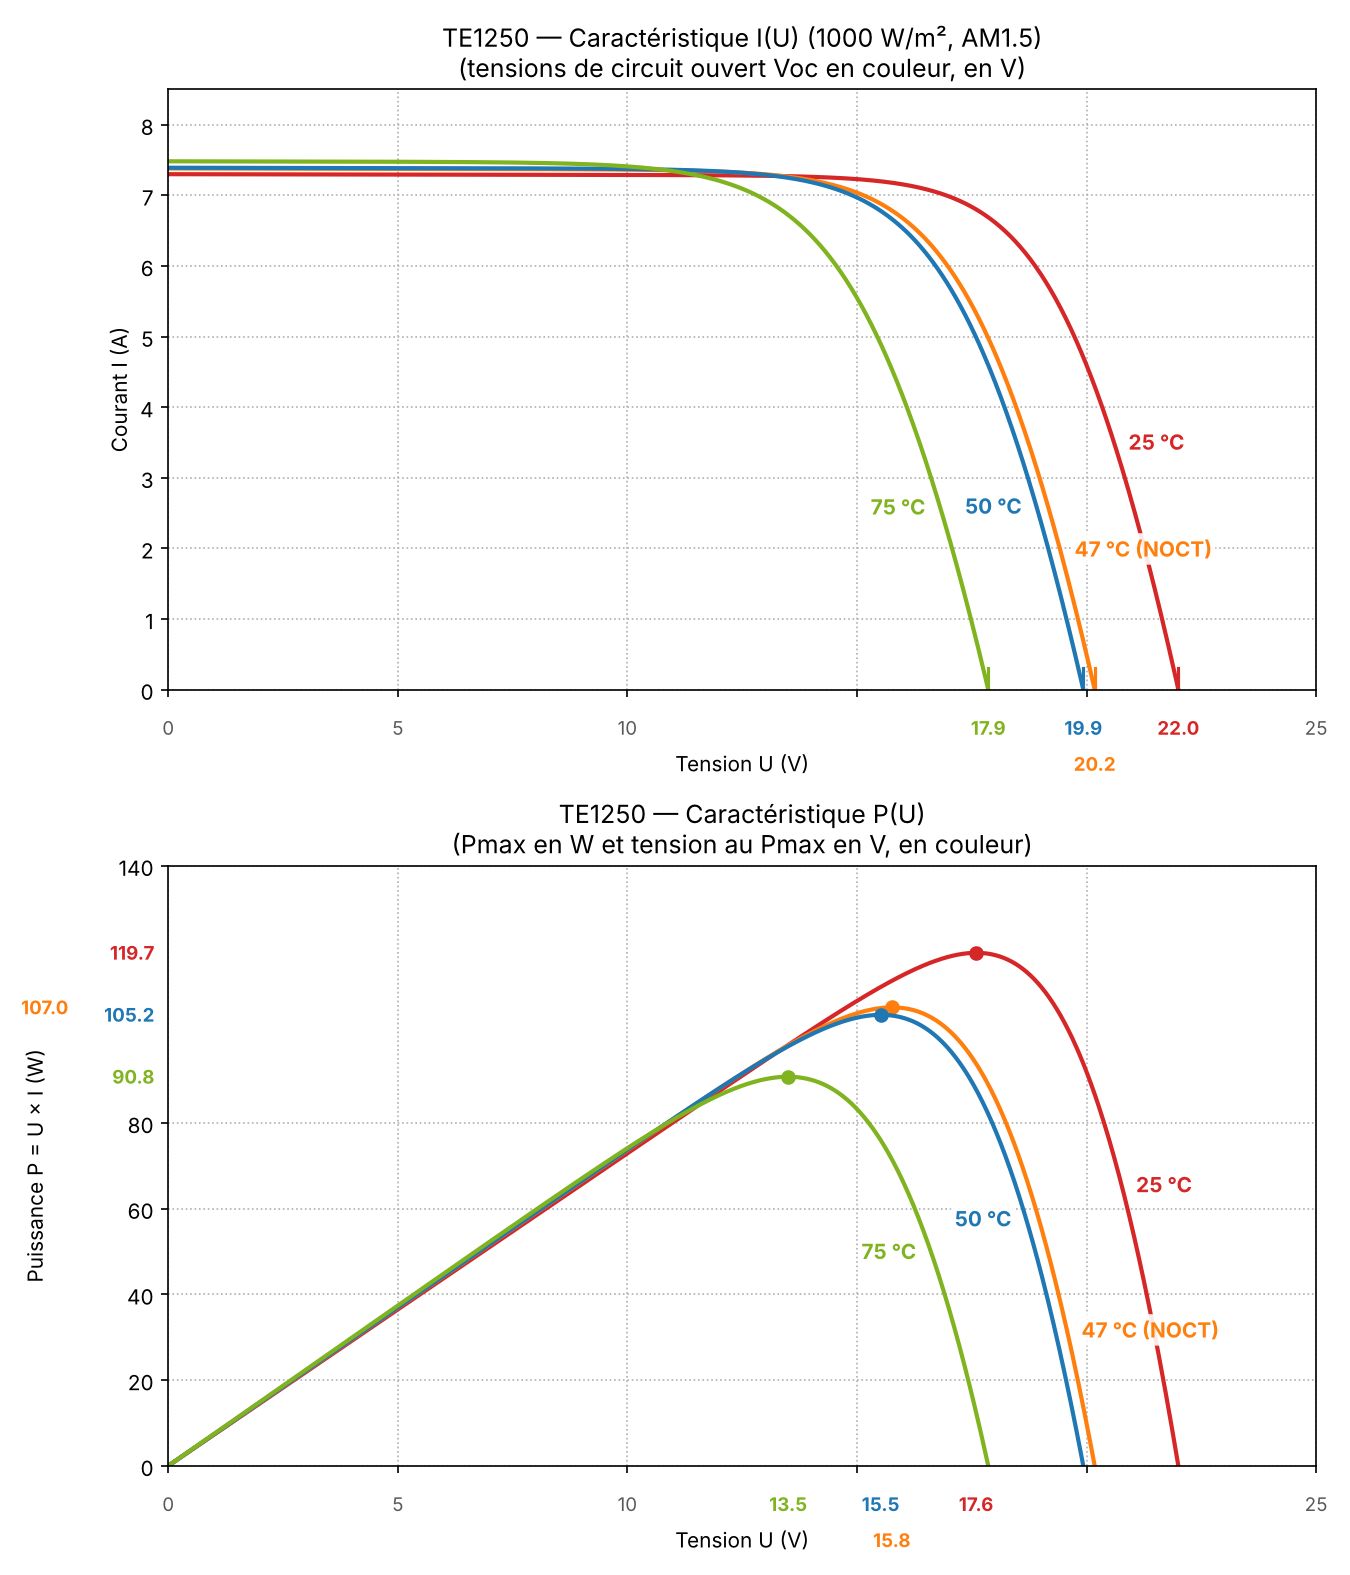
\includegraphics[width=0.62\textwidth]{img/elec/te1250_etude.png}
\caption{Caractéristiques $I(U)$ et $P(U)$ du TE1250 sous \qty{1000}{W/m^2}, reprises de mon étude électrique de départ.}
\end{figure}

\naturecalc[30]{théorie (formule démontrée, valeurs de fiches techniques et hypothèses ; rien de mesuré)}
\begin{demonstration}[puissance et tension du panneau selon la température]
\resultat{P_{\max}(T_c) = P_c\,[1 + \gamma_P\,(T_c - \qty{25}{\celsius})] \qquad k_T = 0{,}855}
Je note $T_c$ la température des cellules, en °C, $P_{\max}(T_c)$ la puissance maximale du panneau à cette température, en watts, et $\gamma_P$ le coefficient de température de la puissance, en 1/°C. Par définition, $\gamma_P$ est la variation relative de puissance par degré :
\begin{align*}
\gamma_P &= \frac{1}{P_c}\,\frac{\mathrm{d}P_{\max}}{\mathrm{d}T_c}
\end{align*}
La fiche donne $\gamma_P$ constant sur la plage de 25 à \qty{75}{\celsius}. La dérivée vaut donc $P_c\,\gamma_P$, constante : la puissance est une fonction affine de $T_c$. Je l'intègre entre \qty{25}{\celsius}, où elle vaut $P_c$, et $T_c$ :
\begin{align*}
P_{\max}(T_c) - P_c &= P_c\,\gamma_P\,(T_c - \qty{25}{\celsius})\\
P_{\max}(T_c) &= P_c\,[1 + \gamma_P\,(T_c - \qty{25}{\celsius})]
\end{align*}
Le facteur de température $k_T$ (sans unité) est le rapport $P_{\max}(T_c)/P_c$. Avec $\gamma_P = -\qty{0,005}{/\celsius}$ et $T_c = \qty{54}{\celsius}$ :
\begin{align*}
k_T &= 1 + \gamma_P\,(T_c - \qty{25}{\celsius})\\
k_T &= 1 - \qty{0,005}{/\celsius} \times (\qty{54}{\celsius} - \qty{25}{\celsius})\\
k_T &= 0{,}855
\end{align*}
La tension au point de puissance maximale se calcule de la même façon avec $\beta_V$, la variation de tension par degré, en V/°C :
\begin{align*}
V_{mp}(T_c) &= V_{mp} + \beta_V\,(T_c - \qty{25}{\celsius})
\end{align*}
À \qty{75}{\celsius} :
\begin{align*}
V_{mp}(\qty{75}{\celsius}) &= \qty{17,6}{V} - \qty{0,080}{V/\celsius} \times (\qty{75}{\celsius} - \qty{25}{\celsius})\\
V_{mp}(\qty{75}{\celsius}) &= \qty{13,6}{V}
\end{align*}
\end{demonstration}

Le tableau compare ce calcul direct aux valeurs lues sur les courbes de mon étude. À \qty{54}{\celsius}, la température n'est pas tracée : je lis la valeur par interpolation linéaire entre les courbes de \qty{50}{\celsius} et \qty{75}{\celsius}, par exemple $\qty{105,2}{W} + (\qty{90,8}{W} - \qty{105,2}{W}) \times (54 - 50)/(75 - 50) \approx \qty{102,9}{W}$.

\begin{table}[H]
\centering
\small
\begin{tabular}{|c|c|c|c|c|c|}
\hline
\textbf{$T_c$} & \textbf{$P_{\max}$ calcul (W)} & \textbf{$P_{\max}$ courbes (W)} & \textbf{Écart} & \textbf{$V_{mp}$ calcul (V)} & \textbf{$V_{mp}$ courbes (V)} \\
\hline
\qty{25}{\celsius} & 120,0 & 119,7 & $+$0,3\,\% & 17,6 & 17,6 \\
\hline
\qty{47}{\celsius} & 106,8 & 107,0 & $-$0,2\,\% & 15,8 & 15,8 \\
\hline
\qty{50}{\celsius} & 105,0 & 105,2 & $-$0,2\,\% & 15,6 & 15,5 \\
\hline
\qty{54}{\celsius} & 102,6 & 102,9 (interpolé) & $-$0,3\,\% & 15,3 & 15,2 (interpolé) \\
\hline
\qty{75}{\celsius} & 90,0 & 90,8 & $-$0,9\,\% & 13,6 & 13,5 \\
\hline
\end{tabular}
\caption{Calcul direct sur le panneau entier et valeurs de mon étude électrique de départ.}
\end{table}

Le calcul direct reste à moins de \qty{1}{\percent} des courbes : il me suffit pour dimensionner. Même à \qty{75}{\celsius}, $V_{mp} = \qty{13,6}{V}$ reste au-dessus de la tension de charge d'une batterie \qty{12}{V} vide : le régulateur MPPT\ix{19} peut toujours charger. C'est la principale raison d'utiliser un régulateur MPPT\ix{19} plutôt qu'une simple liaison directe.

\Needspace{36\baselineskip}\subsubsection*{L'énergie produite et la puissance crête nécessaire}

\naturecalc[30]{théorie (formule démontrée, valeurs de fiches techniques et hypothèses ; rien de mesuré)}
\begin{demonstration}[énergie produite à partir de l'irradiation journalière]
\resultat{E_{prod} = P_c\,\dfrac{H}{G_{STC}}\; k_T\, k_{tol}\, k_s\, k_{MPPT\ix{19}}\, k_{câbles}\, k_{bat}}
Je note $G_{STC} = \qty{1000}{W/m^2}$ l'éclairement des conditions standard, $G(t)$ l'éclairement à l'instant $t$, $H$ l'irradiation journalière, en Wh/m$^2$/j, et $E_{th}$ l'énergie théorique sans perte, en Wh/j. La puissance d'un panneau est proportionnelle à l'éclairement ; à $G_{STC}$ elle vaut $P_c$ :
\begin{align*}
P(t) &= P_c\,\frac{G(t)}{G_{STC}}
\end{align*}
J'intègre sur la journée :
\begin{align*}
E_{th} &= \int_{jour} P(t)\,\mathrm{d}t\\
E_{th} &= \frac{P_c}{G_{STC}} \int_{jour} G(t)\,\mathrm{d}t
\end{align*}
L'intégrale de l'éclairement sur la journée est l'irradiation journalière $H$ :
\begin{align*}
E_{th} &= P_c\,\frac{H}{G_{STC}}
\end{align*}
Le rapport $H/G_{STC}$ est un nombre d'heures, appelé heures équivalentes de plein soleil. Les pertes réelles se multiplient, chacune s'appliquant à ce qui reste après la précédente :
\begin{align*}
E_{prod} &= E_{th}\; k_T\; k_{tol}\; k_s\; k_{MPPT}\; k_{câbles}\; k_{bat}
\end{align*}
\end{demonstration}

Les facteurs retenus sont les suivants. Le facteur $k_T = 0{,}855$ vient de la température des cellules (calcul précédent). Le facteur $k_{tol} = 117{,}5/120 = 0{,}9792$ tient compte de la tolérance de fabrication (puissance minimale garantie de l'étiquette). Le facteur $k_s = 0{,}95$ tient compte des salissures, du sel marin, de la poussière et d'une orientation imparfaite. Le facteur $k_{MPPT} = 0{,}95$ est le rendement du régulateur (la fiche annonce jusqu'à \qty{97}{\percent}). Le facteur $k_{câbles} = 0{,}98$ tient compte des chutes de tension dans les câbles (partie 5.7). Le facteur $k_{bat}$ est le rendement énergétique de la charge puis de la décharge de la batterie : $0{,}95$ en LiFePO4 et $0{,}85$ en plomb AGM. Il est appliqué à toute l'énergie, alors qu'une partie est consommée directement le jour : c'est prudent. Le produit de tous ces facteurs est le rapport de performance $PR$ (sans unité).

\naturecalc[34]{théorie (formule démontrée, valeurs de fiches techniques et hypothèses ; rien de mesuré)}
\begin{demonstration}[puissance crête nécessaire]
\resultat{P_{c,\min} = \dfrac{E_j\,G_{STC}}{H\,PR} \approx \qty{99,9}{Wc}\ \text{(AGM)}\quad\text{ou}\quad \qty{89,3}{Wc}\ \text{(LiFePO4)}}
Je cherche la plus petite puissance crête pour laquelle la production du pire mois égale le besoin journalier $E_j$ (en Wh/j). Je pars de la formule de l'énergie produite, écrite avec $PR$ :
\begin{align*}
E_{prod} &= P_c\,\frac{H}{G_{STC}}\,PR
\end{align*}
Je pose $E_{prod} = E_j$ et j'isole $P_c$ :
\begin{align*}
E_j &= P_{c,\min}\,\frac{H}{G_{STC}}\,PR\\
P_{c,\min} &= \frac{E_j\,G_{STC}}{H\,PR}
\end{align*}
Je calcule d'abord le rapport de performance, avec $k_{bat} = 0{,}85$ pour le plomb AGM puis $0{,}95$ pour le LiFePO4 :
\begin{align*}
PR_{AGM} &= 0{,}855 \times 0{,}9792 \times 0{,}95 \times 0{,}95 \times 0{,}98 \times 0{,}85\\
PR_{AGM} &\approx 0{,}6294\\
PR_{LFP} &= 0{,}855 \times 0{,}9792 \times 0{,}95 \times 0{,}95 \times 0{,}98 \times 0{,}95\\
PR_{LFP} &\approx 0{,}7035
\end{align*}
Avec $E_j = \qty{226,7}{Wh/j}$ et $H = \qty{3607}{Wh/m^2/j}$ :
\begin{align*}
P_{c,\min,AGM} &= \frac{\qty{226,7}{Wh/j} \times \qty{1000}{W/m^2}}{\qty{3607}{Wh/m^2/j} \times 0{,}6294}\\
P_{c,\min,AGM} &\approx \qty{99,9}{W}\\
P_{c,\min,LFP} &= \frac{\qty{226,7}{Wh/j} \times \qty{1000}{W/m^2}}{\qty{3607}{Wh/m^2/j} \times 0{,}7035}\\
P_{c,\min,LFP} &\approx \qty{89,3}{W}
\end{align*}
\end{demonstration}

Il me faut donc un panneau d'au moins \qty{100}{Wc} avec mes batteries au plomb (\qty{89}{Wc} en LiFePO4). Le TE1250 de \qty{120}{Wc} convient. L'ancien panneau SLP055 de \qty{55}{Wc} ne convient pas : avec les mêmes facteurs (hors tolérance), il produirait $\qty{55}{W} \times \qty{3,607}{h/j} \times 0{,}6428 \approx \qty{127,5}{Wh/j}$ en AGM, soit moins que le besoin de \qty{226,7}{Wh/j}. Il ne peut servir que d'appoint.

\naturecalc[22]{théorie (formule démontrée, valeurs de fiches techniques et hypothèses ; rien de mesuré)}
\begin{demonstration}[énergie produite par le TE1250 le pire mois]
\resultat{E_{prod} \approx \qty{272,4}{Wh/j}\ \text{(AGM)} \quad\text{et}\quad \qty{304,5}{Wh/j}\ \text{(LiFePO4)}}
Irradiation du pire mois : $H = \qty{3,607}{kWh/m^2/j}$.
\begin{align*}
E_{th} &= \qty{120}{W} \times \frac{\qty{3607}{Wh/m^2/j}}{\qty{1000}{W/m^2}}\\
E_{th} &= \qty{120}{W} \times \qty{3,607}{h/j}\\
E_{th} &= \qty{432,84}{Wh/j}
\end{align*}
Plomb AGM :
\begin{align*}
E_{prod,AGM} &= \qty{432,84}{Wh/j} \times 0{,}6294\\
E_{prod,AGM} &\approx \qty{272,4}{Wh/j}
\end{align*}
LiFePO4 :
\begin{align*}
E_{prod,LFP} &= \qty{432,84}{Wh/j} \times 0{,}7035\\
E_{prod,LFP} &\approx \qty{304,5}{Wh/j}
\end{align*}
\end{demonstration}

\naturecalc[20]{théorie (formule démontrée, valeurs de fiches techniques et hypothèses ; rien de mesuré)}
\begin{demonstration}[marge du panneau]
\resultat{m = \dfrac{E_{prod}}{E_j} - 1 \approx +20\,\%\ \text{(AGM)}\quad\text{et}\quad +34\,\%\ \text{(LiFePO4)}}
Je note $m$ la marge (sans unité), c'est-à-dire la part de production en plus du besoin :
\begin{align*}
m &= \frac{E_{prod}}{E_j} - 1
\end{align*}
Application :
\begin{align*}
m_{AGM} &= \frac{\qty{272,4}{Wh/j}}{\qty{226,7}{Wh/j}} - 1 \approx 0{,}20 = +20\,\%\\
m_{LFP} &= \frac{\qty{304,5}{Wh/j}}{\qty{226,7}{Wh/j}} - 1 \approx 0{,}34 = +34\,\%
\end{align*}
\end{demonstration}

Je fais le même calcul pour chaque mois, avec le même $PR$ (en été l'air est plus chaud et $PR$ baisse de quelques pour cent, mais l'irradiation est alors bien plus forte : cela ne change pas le pire mois).

\begin{table}[H]
\centering
\small
\begin{tabular}{|l|c|c|c|}
\hline
\textbf{Mois} & \textbf{$H_m$ (kWh/m$^2$/j)} & \textbf{$E_{prod}$ AGM (Wh/j)} & \textbf{Marge $m$} \\
\hline
Janvier & 5,39 & 407,0 & $+$80\,\% \\
\hline
Février & 5,47 & 413,5 & $+$82\,\% \\
\hline
Mars & 5,30 & 400,6 & $+$77\,\% \\
\hline
Avril & 4,54 & 342,7 & $+$51\,\% \\
\hline
Mai & 3,95 & 298,4 & $+$32\,\% \\
\hline
\textbf{Juin} & \textbf{3,61} & \textbf{272,4} & \textbf{$+$20\,\%} \\
\hline
Juillet & 3,77 & 284,8 & $+$26\,\% \\
\hline
Août & 4,33 & 326,9 & $+$44\,\% \\
\hline
Septembre & 4,79 & 362,0 & $+$60\,\% \\
\hline
Octobre & 5,10 & 385,0 & $+$70\,\% \\
\hline
Novembre & 5,34 & 403,2 & $+$78\,\% \\
\hline
Décembre & 5,38 & 406,5 & $+$79\,\% \\
\hline
\end{tabular}
\caption{Production du TE1250 (plomb AGM) et marge sur le besoin de \qty{226,7}{Wh/j}, mois par mois.}
\end{table}

La figure montre la même chose : tous les mois dépassent le besoin, et juin est le plus juste.

\begin{figure}[H]
\centering
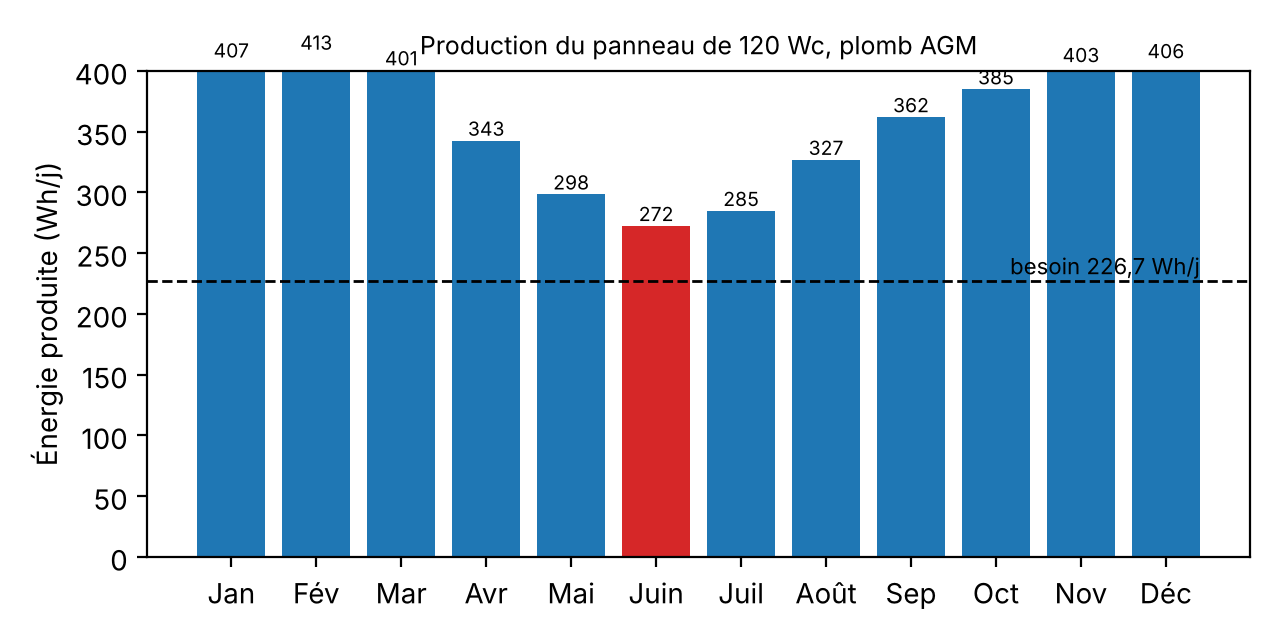
\includegraphics[width=0.78\textwidth]{img/prod_mensuelle.png}
\caption{Énergie produite chaque mois par le TE1250 (plomb AGM), comparée au besoin de \qty{226,7}{Wh/j}. Juin, le pire mois, est en rouge.}
\end{figure}

\subsubsection*{Conclusion sur le panneau}

Je peux maintenant répondre à la question de départ : le panneau fournit-il l'énergie dont la tour a besoin ? Je compare la production du pire mois au besoin journalier, puis je cherche la limite au-delà de laquelle le panneau ne suffirait plus.

\textbf{Oui, le panneau TE1250 de \qty{120}{Wc} suffit.} Le pire mois (juin), il fournit \qty{272,4}{Wh/j} avec mes batteries au plomb, pour un besoin de \qty{226,7}{Wh/j}. Il reste donc \qty{45,7}{Wh/j} de marge, soit $+20\,\%$. Cette marge sert à recharger les batteries après un jour couvert.

\naturecalc[24]{théorie (valeurs de fiches techniques et données d'ensoleillement ; rien de mesuré)}
\begin{demonstration}[limite de la conclusion]
\resultat{t_{max} \approx \qty{9,1}{h/j}}
La marge est la production moins le besoin :
\begin{align*}
\Delta E &= \qty{272,4}{Wh/j} - \qty{226,7}{Wh/j}\\
\Delta E &= \qty{45,7}{Wh/j}
\end{align*}
Je cherche la durée de marche $t_{max}$ de la pompe, en heures par jour, pour laquelle le besoin égale la production du pire mois. Le besoin hors pompe vaut \qty{97,38}{Wh/j} (électronique \qty{91,81}{Wh/j}, doseuses \qty{0,96}{Wh/j} et MPPT\ix{19} \qty{4,61}{Wh/j}). La pompe et son MOSFET\ix{15} consomment $\qty{19}{W} + \qty{0,154}{W} = \qty{19,154}{W}$ :
\begin{align*}
\qty{97,38}{Wh/j} + \qty{19,154}{W} \times t_{max} &= \qty{272,4}{Wh/j}\\
\qty{19,154}{W} \times t_{max} &= \qty{272,4}{Wh/j} - \qty{97,38}{Wh/j}\\
\qty{19,154}{W} \times t_{max} &= \qty{175,02}{Wh/j}\\
t_{max} &= \frac{\qty{175,02}{Wh/j}}{\qty{19,154}{W}}\\
t_{max} &\approx \qty{9,1}{h/j}
\end{align*}
Le planning retenu (\qty{6,75}{h/j}) est donc inférieur à cette limite.
\end{demonstration}

Cette conclusion tient à trois conditions. La pompe doit suivre le planning de l'étude (\qty{15}{min} de marche et \qty{15}{min} d'arrêt le jour, trois marches la nuit) : au-delà d'environ \qty{9}{h} de marche par jour en juin, le panneau ne suffirait plus. Le panneau doit rester propre et sans ombre. Enfin, un jour très couvert ne donne qu'environ \qty{90,6}{Wh/j} : ce jour-là, le panneau seul ne couvre pas le besoin, et ce sont les batteries qui prennent le relais (partie 5.5).

C'est une conclusion théorique : le relevé d'une journée complète (mesure M3) doit la confirmer. Le 12 novembre, j'ai seulement constaté que le panneau charge bien la batterie.

\begin{aretenir}
Pour couvrir \qty{226,7}{Wh/j} le pire mois, il faut au moins \qty{100}{Wc} avec des batteries au plomb. Le pire mois est juin, avec \qty{3,61}{kWh/m^2/j} sur un plan horizontal (Solargis). Le TE1250 de \qty{120}{Wc} fournit alors \qty{272,4}{Wh/j} en plomb AGM (\qty{304,5}{Wh/j} en LiFePO4) : marge de $+20\,\%$ ($+34\,\%$ en LiFePO4). Le panneau est suffisant ; le SLP055 seul ne l'est pas. La pompe pourrait marcher jusqu'à \qty{9,1}{h/j} en juin avant que le panneau ne suffise plus.
\end{aretenir}
\tcbset{enobox/.append style={breakable}}


\Needspace{8\baselineskip}\subsection{Le dimensionnement des batteries}

\subsubsection*{LiFePO4 ou plomb AGM : les deux cas}

Le cahier des charges indique des batteries LiFePO4, alors que la version 1 de l'étude les supposait au plomb AGM. Les deux technologies se comportent très différemment ; le tableau donne les valeurs retenues pour chacune.

\begin{table}[H]
\centering
\small
\begin{tabular}{|l|c|c|}
\hline
\textbf{Grandeur} & \textbf{LiFePO4} & \textbf{Plomb AGM} \\
\hline
Tension nominale de calcul $U_B$ & \qty{12,8}{V} & \qty{12,0}{V} \\
\hline
Profondeur de décharge admise (DoD\ix{27}) & 80\,\% & 50\,\% \\
\hline
Rendement énergétique charge et décharge & 0,95 & 0,85 \\
\hline
Courant de charge admis (usage courant) & $0{,}5\,C$ & $0{,}25\,C$ \\
\hline
Tension de charge (absorption) & \qtyrange{14,2}{14,6}{V} & \qtyrange{14,4}{14,7}{V} \\
\hline
Tension de maintien (floating) & aucune ou \qty{13,6}{V} & \qtyrange{13,5}{13,8}{V} \\
\hline
Tension au repos, batterie pleine & environ \qty{13,4}{V} & environ \qty{12,8}{V} \\
\hline
Tension au repos, batterie vide & environ \qty{12,0}{V} & environ \qty{11,9}{V} (à 50\,\%) \\
\hline
Protection interne (BMS) & oui, en général & non \\
\hline
Énergie nominale (\qty{23}{Ah}) & \qty{294,4}{Wh} & \qty{276,0}{Wh} \\
\hline
Énergie utilisable (\qty{23}{Ah}) & \qty{235,5}{Wh} & \qty{138,0}{Wh} \\
\hline
\end{tabular}
\caption{Comparaison des deux technologies de batterie, pour \qty{23}{Ah} au total.}
\end{table}

\begin{attention}
À vérifier avant tout raccordement. Il faut lire sur l'étiquette de chaque batterie sa technologie (LiFePO4, « Lithium Iron Phosphate », ou « SLA, AGM, Lead Acid »). Mettre en parallèle deux technologies différentes est interdit : les tensions de charge, les courbes de décharge et les protections sont différentes, et l'une des deux serait surchargée ou détruite. Si les deux batteries ne sont pas de la même technologie, il faut n'en utiliser qu'une, ou en remplacer une. Il faut aussi régler le régulateur MPPT\ix{19} sur le type de batterie réel (profil lithium ou plomb).
\end{attention}

\naturecalc{théorie (formule démontrée, valeurs de fiches techniques et hypothèses ; rien de mesuré)}
\begin{demonstration}[énergie utilisable d'une batterie]
\resultat{E_u = U_B\, C\; \mathrm{DoD\ix{27}}}
Je note $C$ la capacité, en ampères-heures, $U_B$ la tension moyenne, en volts, $I$ le courant, en ampères, $\Delta t$ la durée, en heures, et DoD\ix{27} la profondeur de décharge admise (sans unité). Une capacité $C$ délivrée sous la tension moyenne $U_B$ correspond à l'énergie : avec $P = U_B\, I$ et $C = I\,\Delta t$, et $E = P\,\Delta t$ (même raisonnement que pour un composant),
\begin{align*}
E_{nom} &= U_B\, I\,\Delta t\\
E_{nom} &= U_B\, C
\end{align*}
On ne s'autorise à prélever que la fraction DoD\ix{27}, pour préserver la durée de vie :
\begin{align*}
E_u &= U_B\, C\; \mathrm{DoD}
\end{align*}
Deux batteries de même tension en parallèle additionnent leurs capacités (les courants s'additionnent à tension égale) :
\begin{align*}
C &= C_1 + C_2\\
C &= \qty{6}{Ah} + \qty{17}{Ah}\\
C &= \qty{23}{Ah}
\end{align*}
Application aux deux technologies :
\begin{align*}
E_{u,LFP} &= \qty{12,8}{V} \times \qty{23}{Ah} \times 0{,}80 = \qty{235,5}{Wh}\\
E_{u,AGM} &= \qty{12,0}{V} \times \qty{23}{Ah} \times 0{,}50 = \qty{138,0}{Wh}
\end{align*}
\end{demonstration}

\subsubsection*{L'autonomie de nuit}

La nuit compte 14 heures sans production utile (de 17 h à 7 h, hypothèse prudente pour juin). Pendant cette période, la circulation tourne 7 fois \qty{15}{min} (à 17 h, 17 h 30, 21 h, 0 h, 3 h, 6 h et 6 h 30). Elle représente donc $t_{c,nuit} = 7 \times \qty{0,25}{h} = \qty{1,75}{h}$ de marche. C'est le même programme que dans la partie 5.3 : il compte $\qty{6}{h}$ de marche entre 6 h et 18 h et $\qty{0,75}{h}$ la nuit (21 h, 0 h, 3 h), soit $\qty{6,75}{h}$ par jour. Ici, la nuit est comptée de 17 h à 7 h, donc elle contient en plus les marches de 17 h, 17 h 30, 6 h et 6 h 30 (4 fois \qty{0,25}{h}) : $\qty{0,75}{h} + \qty{1,00}{h} = \qty{1,75}{h}$. Le total journalier reste le même.

\naturecalc{théorie (formule démontrée, valeurs de fiches techniques et hypothèses ; rien de mesuré)}
\begin{demonstration}[énergie consommée la nuit]
\resultat{E_n \approx \qty{89,8}{Wh}\ \Rightarrow\ \dfrac{E_n}{E_u} = 65\,\%\ \text{(AGM)}\ \text{ou}\ 38\,\%\ \text{(LiFePO4)}}
Pendant les 14 heures, l'électronique et le régulateur consomment en permanence ; la pompe consomme en plus pendant \qty{1,75}{h}, avec ses pertes MOSFET\ix{15} :
\begin{align*}
E_n &= (P_{12,e} + P_{MPPT}) \times \qty{14}{h} + (P_c + P_1) \times t_{c,nuit}\\
E_n &= (\qty{3,825}{W} + \qty{0,192}{W}) \times \qty{14}{h} + (\qty{19}{W} + \qty{0,154}{W}) \times \qty{1,75}{h}\\
E_n &= \qty{56,24}{Wh} + \qty{33,52}{Wh}\\
E_n &= \qty{89,76}{Wh}\\
E_n &\approx \qty{89,8}{Wh}
\end{align*}
Part de l'énergie utilisable consommée la nuit :
\begin{align*}
\frac{E_n}{E_{u,LFP}} &= \frac{\qty{89,8}{Wh}}{\qty{235,5}{Wh}} = 38\,\%\\
\frac{E_n}{E_{u,AGM}} &= \frac{\qty{89,8}{Wh}}{\qty{138,0}{Wh}} = 65\,\%
\end{align*}
La profondeur de décharge réelle au matin, rapportée à l'énergie nominale, vaut $\qty{89,8}{Wh}/\qty{294,4}{Wh} = 30\,\%$ en LiFePO4 ou $\qty{89,8}{Wh}/\qty{276,0}{Wh} = 33\,\%$ en AGM. La nuit passe donc, dans les deux cas, sans dépasser la profondeur de décharge admise.
\end{demonstration}

\subsubsection*{Les jours sans soleil}

\naturecalc{théorie (formule démontrée, valeurs de fiches techniques et hypothèses ; rien de mesuré)}
\begin{demonstration}[autonomie sans aucune production]
\resultat{N_0 = \dfrac{E_u}{E_j} \approx \qty{0,61}{j}\ \text{(AGM)}\ \text{ou}\ \qty{1,04}{j}\ \text{(LiFePO4)}}
Je note $N_0$ le nombre de jours que tient la batterie sans aucune production (sans unité de temps autre que le jour). Chaque jour, la tour consomme $E_j$ : le nombre de jours est l'énergie utilisable divisée par la consommation d'un jour.
\begin{align*}
N_0 &= \frac{E_u}{E_j}\\
N_{0,LFP} &= \frac{\qty{235,5}{Wh}}{\qty{226,7}{Wh/j}} \approx \qty{1,04}{j}\\
N_{0,AGM} &= \frac{\qty{138,0}{Wh}}{\qty{226,7}{Wh/j}} \approx \qty{0,61}{j}
\end{align*}
\end{demonstration}

\naturecalc{théorie (formule démontrée, valeurs de fiches techniques et hypothèses ; rien de mesuré)}
\begin{demonstration}[autonomie par jours très couverts]
\resultat{N_c = \dfrac{E_u}{E_j - E_c} \approx \qty{1,0}{j}\ \text{(AGM)}\ \text{ou}\ \qty{1,9}{j}\ \text{(LiFePO4)}}
Un jour très couvert apporte encore environ $H_c = \qty{1,2}{kWh/m^2/j}$ (hypothèse). Je note $E_c$ la production de ce jour, en Wh/j, $D$ le déficit journalier, en Wh/j, et $N_c$ le nombre de jours couverts consécutifs supportés en partant de batteries pleines. Le déficit est la consommation moins la production, et le nombre de jours est l'énergie utilisable divisée par le déficit :
\begin{align*}
D &= E_j - E_c\\
N_c &= \frac{E_u}{D}
\end{align*}
Cas LiFePO4 ($PR = 0{,}703$) :
\begin{align*}
E_{c,LFP} &= \qty{120}{W} \times \qty{1,2}{h/j} \times 0{,}703 \approx \qty{101,2}{Wh/j}\\
D_{LFP} &= \qty{226,7}{Wh/j} - \qty{101,2}{Wh/j} = \qty{125,5}{Wh/j}\\
N_{c,LFP} &= \frac{\qty{235,5}{Wh}}{\qty{125,5}{Wh/j}} \approx \qty{1,9}{j}
\end{align*}
Cas plomb AGM ($PR = 0{,}629$) :
\begin{align*}
E_{c,AGM} &= \qty{120}{W} \times \qty{1,2}{h/j} \times 0{,}629 = \qty{90,6}{Wh/j}\\
D_{AGM} &= \qty{226,7}{Wh/j} - \qty{90,6}{Wh/j} = \qty{136,1}{Wh/j}\\
N_{c,AGM} &= \frac{\qty{138,0}{Wh}}{\qty{136,1}{Wh/j}} \approx \qty{1,0}{j}
\end{align*}
\end{demonstration}

\textbf{Interprétation.} Les batteries couvrent largement la nuit, mais pas une longue période couverte. Le programme du Raspberry Pi doit donc prévoir un \textbf{mode sobriété} déclenché sur la tension de la batterie mesurée par l'INA260\ix{22} (par exemple sous \qty{12,9}{V} au repos en LiFePO4) : circulation réduite à \qty{10}{min} par heure le jour, nuit inchangée. La consommation descend alors vers \qty{150}{Wh/j} : la circulation tourne $12 \times \qty{10}{min} = \qty{2}{h}$ le jour et \qty{0,75}{h} la nuit, soit \qty{2,75}{h}, d'où $\qty{19}{W} \times \qty{2,75}{h} = \qty{52,25}{Wh/j}$ pour la pompe, auxquels s'ajoutent \qty{91,81}{Wh/j} d'électronique, \qty{0,42}{Wh/j} de pertes MOSFET\ix{15}, \qty{0,96}{Wh/j} de doseuses et \qty{4,61}{Wh/j} d'autoconsommation du MPPT\ix{19}, ce qui fait $\qty{150,05}{Wh/j}$.

\naturecalc{théorie (formule démontrée, valeurs de fiches techniques et hypothèses ; rien de mesuré)}
\begin{demonstration}[capacité pour deux jours sans soleil]
\resultat{C_{2j} = \dfrac{2\,E_j}{U_B\,\mathrm{DoD\ix{27}}} \approx \qty{76}{Ah}\ \text{(AGM)}\ \text{ou}\ \qty{44}{Ah}\ \text{(LiFePO4)}}
Pour tenir $N = 2$ jours sans soleil, il faut une énergie utilisable $E_u = N\,E_j$. D'après la démonstration de l'énergie utilisable, $E_u = U_B\, C\,\mathrm{DoD}$, d'où la capacité nécessaire :
\begin{align*}
N\,E_j &= U_B\, C_{2j}\,\mathrm{DoD}\\
C_{2j} &= \frac{N\,E_j}{U_B\,\mathrm{DoD}}
\end{align*}
\begin{align*}
C_{2j,LFP} &= \frac{2 \times \qty{226,7}{Wh}}{\qty{12,8}{V} \times 0{,}80} \approx \qty{44}{Ah}\\
C_{2j,AGM} &= \frac{2 \times \qty{226,7}{Wh}}{\qty{12,0}{V} \times 0{,}50} \approx \qty{76}{Ah}
\end{align*}
La batterie de \qty{23}{Ah} est donc trop petite pour deux jours sans soleil complet : le mode sobriété est indispensable.
\end{demonstration}

\subsubsection*{La mise en parallèle de deux batteries de capacités différentes}

\naturecalc{théorie (formule démontrée, valeurs de fiches techniques et hypothèses ; rien de mesuré)}
\begin{demonstration}[partage du courant entre deux batteries en parallèle]
\resultat{I_k = I\,\dfrac{C_k}{C_1 + C_2}}
Chaque batterie se modélise par une force électromotrice $E_k$ en série avec une résistance interne $R_k$. Je note $I_k$ le courant de la batterie $k$, en ampères, et $I = I_1 + I_2$ le courant total. En parallèle, elles ont la même tension $U$ aux bornes :
\begin{align*}
U &= E_1 - R_1 I_1 = E_2 - R_2 I_2
\end{align*}
Si les deux batteries sont au même état de charge, $E_1 = E_2$, donc :
\begin{align*}
R_1 I_1 &= R_2 I_2
\end{align*}
Avec $I = I_1 + I_2$, on a $I_2 = I - I_1$, donc $R_1 I_1 = R_2 (I - I_1)$ et :
\begin{align*}
I_1 &= I\,\frac{R_2}{R_1 + R_2}\\
I_2 &= I\,\frac{R_1}{R_1 + R_2}
\end{align*}
Pour une même technologie, la résistance interne est à peu près inversement proportionnelle à la capacité, $R_k = r/C_k$ ($r$ constante). Je remplace :
\begin{align*}
I_1 &= I\,\frac{r/C_2}{r/C_1 + r/C_2}
\end{align*}
Je multiplie haut et bas par $C_1 C_2/r$ :
\begin{align*}
I_1 &= I\,\frac{C_1}{C_1 + C_2}
\end{align*}
Chaque batterie prend une part du courant proportionnelle à sa capacité : elles se chargent et se déchargent au même régime ($I_k/C_k$ identique).

Courant de circulation : si l'on relie deux batteries dont les tensions diffèrent de $\Delta E = E_1 - E_2$, sans charge extérieure, la loi des mailles donne :
\begin{align*}
I_{circ} &= \frac{E_1 - E_2}{R_1 + R_2}
\end{align*}
\end{demonstration}

\naturecalc{théorie (formule démontrée, valeurs de fiches techniques et hypothèses ; rien de mesuré)}
\begin{demonstration}[partage du courant de charge et courant de circulation]
\resultat{I_{B1} \approx \qty{2,32}{A},\quad I_{B2} \approx \qty{6,58}{A},\quad I_{circ} \approx \qty{3,7}{A}}
Je note $I_{ch}$ le courant de charge maximal sortant du régulateur, en ampères. La puissance maximale du panneau, réduite par le rendement du régulateur, charge la batterie sous la tension $U_B$ :
\begin{align*}
I_{ch} &= \frac{P_c\, k_{MPPT}}{U_B}\\
I_{ch} &= \frac{\qty{120}{W} \times 0{,}95}{\qty{12,8}{V}}\\
I_{ch} &\approx \qty{8,9}{A}
\end{align*}
(Avec $U_B = \qty{12,0}{V}$ en plomb AGM, le même calcul donne $\qty{120}{W} \times 0{,}95/\qty{12,0}{V} = \qty{9,5}{A}$.) D'après la démonstration précédente, le courant de chaque batterie vaut :
\begin{align*}
I_{B1} &= \qty{8,9}{A} \times \frac{\qty{6}{Ah}}{\qty{23}{Ah}} \approx \qty{2,32}{A}\\
I_{B2} &= \qty{8,9}{A} \times \frac{\qty{17}{Ah}}{\qty{23}{Ah}} \approx \qty{6,58}{A}
\end{align*}
Le régime de charge de chaque batterie vaut $\qty{2,32}{A}/\qty{6}{Ah} = \qty{6,58}{A}/\qty{17}{Ah} \approx 0{,}39\,C$. En LiFePO4, $0{,}39\,C$ est inférieur à $0{,}5\,C$ : c'est acceptable. En plomb AGM, $0{,}39\,C$ est supérieur à $0{,}25\,C$ (et à $0{,}41\,C$ avec \qty{9,5}{A}) : la charge est un peu trop forte en plein soleil, ce qui accélère le vieillissement. Il faut alors limiter le courant de charge à environ $0{,}25 \times \qty{23}{Ah} \approx \qty{5,8}{A}$ si le régulateur le permet (à vérifier dans sa notice), ou accepter un vieillissement plus rapide.

Courant de circulation si l'on relie les batteries avec $\Delta E = \qty{0,3}{V}$ d'écart. Je suppose $R_{B1} = \qty{60}{m\ohm}$ pour la batterie de \qty{6}{Ah} (hypothèse, sans fiche technique : à mesurer), donc, par proportion inverse à la capacité, $R_{B2} = \qty{60}{m\ohm} \times 6/17 \approx \qty{21}{m\ohm}$ :
\begin{align*}
I_{circ} &= \frac{\qty{0,3}{V}}{\qty{0,060}{\ohm} + \qty{0,021}{\ohm}}\\
I_{circ} &\approx \qty{3,7}{A}
\end{align*}
Un faible écart de tension provoque déjà un courant important : d'où les précautions qui suivent.
\end{demonstration}

\textbf{Précautions de mise en parallèle.} Je commence par exiger la même technologie et la même tension nominale, ce qui est obligatoire. Ensuite, je charge chaque batterie séparément jusqu'à pleine charge, puis je vérifie au multimètre un écart de tension inférieur à \qty{0,05}{V} avant de les relier. Je place un fusible par batterie ($F_{B1}$, $F_{B2}$), au plus près de la borne $+$ : un court-circuit interne d'une batterie ne doit pas être alimenté par l'autre. J'utilise des câbles de même section et de même longueur entre chaque batterie et le bus. Je fais le raccordement « en diagonale » : le $+$ du bus est pris sur une batterie et le $-$ sur l'autre, pour équilibrer les chutes de tension. En LiFePO4, chaque batterie a son BMS : si l'un coupe, toute la charge passe dans l'autre (voir le choix des fusibles, partie 5.7). Enfin, je remplace les deux batteries ensemble en fin de vie.

\begin{aretenir}
Capacité totale \qty{23}{Ah}. Énergie utilisable : \qty{138,0}{Wh} en plomb AGM (DoD\ix{27} 50\,\%), \qty{235,5}{Wh} en LiFePO4 (DoD\ix{27} 80\,\%). La nuit consomme \qty{89,8}{Wh}, soit 65\,\% (AGM) ou 38\,\% (LiFePO4) de l'énergie utilisable. Autonomie sans soleil : \qty{0,6}{j} (AGM) ou \qty{1,0}{j} (LiFePO4) ; par jours très couverts : \qty{1,0}{j} ou \qty{1,9}{j}. Un mode sobriété piloté par la tension de la batterie est nécessaire. La technologie réelle des deux batteries doit être lue sur leurs étiquettes : jamais deux technologies différentes en parallèle.
\end{aretenir}


\Needspace{8\baselineskip}\subsection{La tension réellement présente sur le réseau \qty{12}{V}}

Je me demande si le régulateur délivre un \qty{12}{V} stable à la tour. La réponse décide du choix du convertisseur et de la tolérance des pompes. Je pars de la fiche du régulateur : sa sortie « charge » est reliée à la batterie, et il ne contient pas de convertisseur de tension qui régule cette sortie. Je cherche donc la tension $U_{bus}$ du réseau, en volts, en fonction de la tension $U_{bat}$ de la batterie, en volts. Je vérifie ensuite que chaque récepteur accepte toute la plage possible.

\naturecalc{théorie (formule démontrée, valeurs de fiches techniques et hypothèses ; rien de mesuré)}
\begin{demonstration}[tension du réseau et plage de fonctionnement]
\resultat{U_{bus} = U_{bat} \quad \text{avec} \quad \qty{11,5}{V} \leq U_{bus} \leq \qty{14,4}{V}}
Les récepteurs (pompes, carte MOSFET\ix{15}, convertisseur UBEC\ix{17}) et la batterie sont reliés aux mêmes deux fils. Deux points reliés par un fil sans résistance sont au même potentiel, donc la différence de potentiel entre les deux fils est la même pour tous :
\begin{align*}
U_{pompes} &= U_{MOSFET} = U_{UBEC}\\
U_{pompes} &= U_{bus}
\end{align*}
Le fil entre la batterie et le réseau a une résistance $R_c$ (en ohms) très faible et traverse un courant $I$ (en ampères). La loi d'Ohm donne la chute de tension dans ce fil :
\[
\Delta U = R_c \times I
\]
La résistance d'un fil de cuivre de longueur $L$ (en mètres), de section $S$ (en \unit{mm^2}) et de résistivité $\rho = \qty{0,0172}{\ohm.mm^2/m}$ vaut :
\begin{align*}
R_c &= \rho \times \frac{L}{S}\\
R_c &= \qty{0,0172}{\ohm.mm^2/m} \times \frac{\qty{1}{m}}{\qty{4}{mm^2}}\\
R_c &\approx \qty{0,0043}{\ohm}
\end{align*}
Pour un fil de \qty{4}{mm^2} et \qty{1}{m} de longueur totale (aller et retour) et un courant de \qty{10}{A} :
\begin{align*}
\Delta U &= \qty{0,0043}{\ohm} \times \qty{10}{A}\\
\Delta U &= \qty{0,043}{V}
\end{align*}
Cette chute est négligeable devant \qty{12}{V}, d'où $U_{bus} = U_{bat}$ à \qty{0,05}{V} près.

La tension de la batterie n'est pas fixe : le régulateur la fait monter à \qty{14,4}{V} pendant l'absorption, la maintient à \qty{13,8}{V}, et coupe la sortie à \qty{11,5}{V} (reconnexion à \qty{12,6}{V}). Les écarts par rapport au \qty{12}{V} nominal valent :
\begin{align*}
\frac{\qty{14,4}{V} - \qty{12}{V}}{\qty{12}{V}} &= \frac{\qty{2,4}{V}}{\qty{12}{V}} = +\,20\,\%\\
\frac{\qty{11,5}{V} - \qty{12}{V}}{\qty{12}{V}} &= \frac{-\qty{0,5}{V}}{\qty{12}{V}} \approx -\,4,2\,\%
\end{align*}
La tension du réseau varie donc de $-4,2\,\%$ à $+20\,\%$ autour de \qty{12}{V}. La largeur de la plage vaut :
\[
\Delta U_{plage} = \qty{14,4}{V} - \qty{11,5}{V} = \qty{2,9}{V}
\]
\end{demonstration}

Il en découle une condition de choix : chaque récepteur doit accepter au moins \qtyrange{11,5}{14,4}{V}. Pour les pompes à \qty{12}{V} et la carte MOSFET\ix{15} (\qtyrange{3}{24}{V}), la plage est acceptée par la carte ; pour les pompes, je mesurerai le courant à \qty{14,4}{V} (mesure M1) car un moteur à courant continu tourne plus vite et consomme plus quand la tension monte. Pour le convertisseur UBEC\ix{17}, la fiche du modèle choisi doit annoncer une plage d'entrée qui contient \qtyrange{11,5}{14,4}{V} : c'est ce critère, et non la valeur \qty{12}{V}, qui fixe le choix. Enfin, le régulateur coupe la sortie à \qty{11,5}{V} : en dessous, tout le réseau s'éteint, y compris le Raspberry Pi, et ne se rallume qu'à \qty{12,6}{V}. Cet écart de \qty{1,1}{V} évite les redémarrages en boucle.

\begin{aretenir}
Brancher une batterie de \qty{12}{V} sur le régulateur ne donne pas un \qty{12}{V} régulé : le réseau suit la batterie, entre \qty{11,5}{V} et \qty{14,4}{V}. C'est donc la plage d'entrée de chaque récepteur qu'il faut vérifier.
\end{aretenir}



\Needspace{8\baselineskip}\subsection{Les sections de câbles et les fusibles}

\subsubsection*{La chute de tension et la section minimale}

Je cherche, pour chaque liaison, la plus petite section de cuivre qui garde la chute de tension sous une limite, puis je prends la section normalisée immédiatement supérieure.

\naturecalc{théorie (formule démontrée, valeurs de fiches techniques et hypothèses ; rien de mesuré)}
\begin{demonstration}[section minimale d'un câble]
\resultat{S \geq \dfrac{2\,\rho\, L\, I}{\varepsilon\, U}}
Je note $\rho$ la résistivité du cuivre, en $\unit{\ohm\,mm^2/m}$, $L$ la longueur de la liaison, en mètres, $S$ la section, en mm$^2$, $I$ le courant, en ampères, $U$ la tension de la ligne, en volts, et $\varepsilon$ la chute de tension relative admise (sans unité). La résistance d'un conducteur de longueur $\ell$ et de section $S$ vaut :
\begin{align*}
R &= \rho\,\frac{\ell}{S}
\end{align*}
Le courant fait l'aller et le retour : pour une liaison de longueur $L$, la longueur de conducteur est $\ell = 2L$ :
\begin{align*}
R &= \frac{2\,\rho\, L}{S}
\end{align*}
La chute de tension se calcule par la loi d'Ohm :
\begin{align*}
\Delta U &= R\, I\\
\Delta U &= \frac{2\,\rho\, L\, I}{S}
\end{align*}
J'impose $\Delta U \leq \varepsilon\, U$ :
\begin{align*}
\frac{2\,\rho\, L\, I}{S} &\leq \varepsilon\, U\\
S &\geq \frac{2\,\rho\, L\, I}{\varepsilon\, U}
\end{align*}
La résistivité du cuivre augmente avec la température $T$ (en °C), avec le coefficient $\alpha_{Cu} = \qty{0,00393}{/\celsius}$ :
\begin{align*}
\rho(T) &= \rho_{20}\left[1 + \alpha_{Cu}\,(T - \qty{20}{\celsius})\right]
\end{align*}
\end{demonstration}

\naturecalc{théorie (formule démontrée, valeurs de fiches techniques et hypothèses ; rien de mesuré)}
\begin{demonstration}[résistivité du cuivre à 60 °C]
\resultat{\rho = \qty{0,0199}{\ohm.mm^2/m}}
Les câbles sont au soleil ou dans le boîtier chaud : je prends $T = \qty{60}{\celsius}$, et $\rho_{20} = \qty{0,0172}{\ohm.mm^2/m}$ :
\begin{align*}
\rho &= \qty{0,0172}{\ohm.mm^2/m} \times \left[1 + \qty{0,00393}{/\celsius} \times (\qty{60}{\celsius} - \qty{20}{\celsius})\right]\\
\rho &= \qty{0,0172}{\ohm.mm^2/m} \times 1{,}1572\\
\rho &\approx \qty{0,0199}{\ohm.mm^2/m}
\end{align*}
\end{demonstration}

\naturecalc{théorie (formule démontrée, valeurs de fiches techniques et hypothèses ; rien de mesuré)}
\begin{demonstration}[section du câble panneau vers régulateur]
\resultat{S \geq \qty{2,97}{mm^2}\ \Rightarrow\ S = \qty{4}{mm^2}}
Avec $L = \qty{5}{m}$, $I = \qty{6,83}{A}$ et $U = \qty{15,26}{V}$ (point de puissance maximale à \qty{54}{\celsius}), et $\varepsilon = 3\,\%$ :
\begin{align*}
S &\geq \frac{2 \times \qty{0,0199}{\ohm.mm^2/m} \times \qty{5}{m} \times \qty{6,83}{A}}{0{,}03 \times \qty{15,26}{V}}\\
S &\geq \frac{\qty{1,359}{\ohm.mm^2.A}}{\qty{0,458}{V}}\\
S &\geq \qty{2,97}{mm^2}
\end{align*}
Je choisis \qty{4}{mm^2} (câble solaire), la section normalisée immédiatement supérieure. La chute réelle vaut alors :
\begin{align*}
\Delta U &= \frac{2 \times \qty{0,0199}{\ohm.mm^2/m} \times \qty{5}{m} \times \qty{6,83}{A}}{\qty{4}{mm^2}}\\
\Delta U &\approx \qty{0,34}{V} \quad (2{,}2\,\%)
\end{align*}
\end{demonstration}

Les autres liaisons se calculent de la même façon. Le tableau donne, pour chacune, la longueur, le courant, la tension, la chute relative admise, la section minimale, la section retenue et la chute réelle.

\begin{table}[H]
\centering
\small
\begin{tabular}{|l|c|c|c|c|c|c|c|}
\hline
\textbf{Liaison} & \textbf{$L$ (m)} & \textbf{$I$ (A)} & \textbf{$U$ (V)} & \textbf{$\varepsilon$} & \textbf{$S_{\min}$ (mm$^2$)} & \textbf{$S$ (mm$^2$)} & \textbf{$\Delta U$ réel} \\
\hline
Panneau vers MPPT\ix{19} & 5,0 & 6,83 & 15,3 & 3\,\% & 2,97 & 4 & 2,2\,\% \\
\hline
MPPT\ix{19} vers INA260\ix{22} vers bus & 0,5 & 8,91 & 12,8 & 1\,\% & 1,38 & 4 & 0,35\,\% \\
\hline
Bus vers B1 (6 Ah) & 0,3 & 2,32 & 12,8 & 0,5\,\% & 0,43 & 2,5 & 0,09\,\% \\
\hline
Bus vers B2 (17 Ah) & 0,3 & 6,58 & 12,8 & 0,5\,\% & 1,23 & 2,5 & 0,25\,\% \\
\hline
Sortie LOAD vers bornier & 0,5 & 2,70 & 12,8 & 1\,\% & 0,42 & 1,5 & 0,28\,\% \\
\hline
Bornier vers circulation & 3,0 & 1,48 & 12,8 & 3\,\% & 0,46 & 1,5 & 0,92\,\% \\
\hline
Bornier vers doseuse & 1,0 & 0,30 & 12,8 & 3\,\% & 0,03 & 0,5 & 0,19\,\% \\
\hline
UBEC\ix{17} vers Pi (\qty{5}{V}) & 0,3 & 1,00 & 5,0 & 2\,\% & 0,12 & 0,5 & 0,48\,\% \\
\hline
\end{tabular}
\caption{Sections de câbles : $\rho = \qty{0,0199}{\ohm.mm^2/m}$ à \qty{60}{\celsius}, chute admise $\varepsilon$ propre à chaque liaison (\qty{3}{\percent} côté panneau et pompes, \qty{1}{\percent} côté batterie, \qty{0,5}{\percent} entre batteries, \qty{2}{\percent} sur le \qty{5}{V}).}
\end{table}

La chute totale du panneau aux batteries vaut environ $2{,}2 + 0{,}35 = \qty{2,6}{\percent}$ au courant maximal, et nettement moins en moyenne sur la journée : le facteur $k_{câbles} = 0{,}98$ est cohérent. Sur le \qty{5}{V} du Pi, une chute supérieure à \qty{0,25}{V} provoque des alertes de sous-tension : le câble court de \qty{0,5}{mm^2} est indispensable (il faut éviter un câble USB fin et long).

\subsubsection*{Les fusibles}

\naturecalc{théorie (formule démontrée, valeurs de fiches techniques et hypothèses ; rien de mesuré)}
\begin{demonstration}[règle de choix d'un fusible]
\resultat{1{,}25\, I_b \leq I_n \leq I_z}
Je note $I_b$ le courant normal maximal dans la ligne, en ampères, $I_n$ le calibre du fusible, en ampères, et $I_z$ le courant admissible du câble protégé, en ampères. Le fusible doit laisser passer le courant normal maximal sans fondre ni vieillir : je prends une marge de 25\,\%.
\begin{align*}
I_n &\geq 1{,}25\, I_b
\end{align*}
Il doit aussi fondre avant que le câble chauffe dangereusement, donc rester sous le courant admissible du câble :
\begin{align*}
1{,}25\, I_b &\leq I_n \leq I_z
\end{align*}
On prend le calibre normalisé immédiatement supérieur à $1{,}25\, I_b$ (valeurs courantes : 1, 2, 3, 4, 5, 7,5, 10, 15, 20 A).
\end{demonstration}

\naturecalc{théorie (formule démontrée, valeurs de fiches techniques et hypothèses ; rien de mesuré)}
\begin{demonstration}[calibres des fusibles]
\resultat{F_{PV} = \qty{10}{A},\ F_{B1} = \qty{5}{A},\ F_{B2} = \qty{15}{A},\ F_2 = \qty{4}{A},\ F_3 = \qty{2}{A}}
$F_{PV}$ (panneau). Le courant maximal est le courant de court-circuit, augmenté à chaud :
\begin{align*}
1{,}25 \times \qty{7,3}{A} &= \qty{9,1}{A}\ \Rightarrow\ I_n = \qty{10}{A}
\end{align*}
C'est aussi le calibre maximal autorisé par l'étiquette du panneau.

$F_{B1}$ (batterie de \qty{6}{Ah}). Courant normal en charge \qty{2,32}{A} :
\begin{align*}
1{,}25 \times \qty{2,32}{A} &= \qty{2,9}{A}\ \Rightarrow\ I_n = \qty{5}{A}\ \text{(conservé)}
\end{align*}
Si le BMS de B2 coupe, les \qty{8,9}{A} de charge passeraient dans B1 : le fusible de \qty{5}{A} fond et protège la petite batterie.

$F_{B2}$ (batterie de \qty{17}{Ah}). Normalement \qty{6,58}{A}, mais jusqu'à \qty{8,9}{A} si B1 est déconnectée :
\begin{align*}
1{,}25 \times \qty{8,9}{A} &= \qty{11,1}{A}\ \Rightarrow\ I_n = \qty{15}{A}\ \text{(conservé)}
\end{align*}
En plomb AGM (\qty{9,5}{A} de charge), $1{,}25 \times \qty{9,5}{A} = \qty{11,9}{A}$ conduit au même calibre de \qty{15}{A}.

$F_2$ (sortie LOAD, toutes les charges). Le courant maximal est celui de la circulation, des trois doseuses ensemble (cas extrême) et de l'électronique :
\begin{align*}
I_b &= \qty{1,48}{A} + 3 \times \qty{0,30}{A} + \qty{0,30}{A}\\
I_b &= \qty{2,68}{A}\\
1{,}25 \times \qty{2,68}{A} &= \qty{3,4}{A}\ \Rightarrow\ I_n = \qty{4}{A}
\end{align*}
La version 1 prévoyait \qty{7,5}{A} avec la pompe d'appoint ; sans elle, \qty{4}{A} protège mieux.

\textbf{Limite de ce calcul.} Il part des courants permanents. Au démarrage, un moteur à courant continu peut absorber brièvement un courant plus grand que son courant nominal, et la fiche de la pompe ne donne pas cette valeur. Je ne peux donc pas valider définitivement le calibre de \qty{4}{A} : je mesurerai le pic de démarrage de la circulation et des doseuses avec l'INA260\ix{22} ou une pince ampèremétrique. Si le pic dure plus de quelques dizaines de millisecondes au-dessus de \qty{4}{A}, je prendrai un fusible temporisé, et je vérifierai dans la fiche de la carte MOSFET\ix{15} qu'elle supporte ce pic.

$F_3$ (entrée de l'UBEC\ix{17}). Le courant d'entrée maximal si l'UBEC\ix{17} fournit ses \qty{3}{A} nominaux se déduit du rendement : $P_{entrée} = P_{sortie}/\eta$, donc $I_{entrée} = P_{sortie}/(\eta\, U_B)$ :
\begin{align*}
I_{entrée,max} &= \frac{\qty{5}{V} \times \qty{3}{A}}{0{,}83 \times \qty{12,8}{V}}\\
I_{entrée,max} &\approx \qty{1,41}{A}\\
1{,}25 \times \qty{1,41}{A} &= \qty{1,8}{A}\ \Rightarrow\ I_n = \qty{2}{A}
\end{align*}
\end{demonstration}

Le tableau suivant donne le calibre retenu pour chaque fusible de la tour.

\begin{table}[H]
\centering
\small
\begin{tabular}{|l|l|c|c|c|}
\hline
\textbf{Fusible} & \textbf{Emplacement} & \textbf{$I_b$ (A)} & \textbf{Calibre v1} & \textbf{Calibre v2} \\
\hline
$F_{PV}$ & panneau, borne $+$ & 7,3 & \qty{10}{A} & \qty{10}{A} \\
\hline
$F_{B1}$ & batterie \qty{6}{Ah}, borne $+$ & 2,32 & \qty{5}{A} & \qty{5}{A} \\
\hline
$F_{B2}$ & batterie \qty{17}{Ah}, borne $+$ & 6,58 (8,9) & \qty{15}{A} & \qty{15}{A} \\
\hline
$F_2$ & sortie LOAD du MPPT\ix{19} & 2,68 & \qty{7,5}{A} & \qty{4}{A} \\
\hline
$F_3$ & entrée de l'UBEC\ix{17} & 0,30 (1,41) & absent & \qty{2}{A} \\
\hline
\end{tabular}
\caption{Calibres des fusibles de la tour.}
\end{table}

\textbf{Autres vérifications.} L'INA260\ix{22} supporte \qty{15}{A} en continu : avec $F_{B2} = \qty{15}{A}$ en amont et \qty{8,9}{A} au maximum en fonctionnement, il est protégé (le régulateur peut débiter \qty{20}{A}, mais le panneau ne peut pas dépasser \qty{7,3}{A} de courant de court-circuit, soit moins de \qty{10}{A} côté batterie). La tension maximale du panneau, le matin frais à $T_c = \qty{20}{\celsius}$, vaut $22{,}0 - 0{,}080 \times (20 - 25) = \qty{22,4}{V}$ : elle est très inférieure aux \qty{70}{V} d'entrée admis par la fiche du régulateur. Chaque canal de la carte 6318 supporte \qty{3,6}{A} en pointe : la circulation (\qty{0,74}{A} par canal) et les doseuses (\qty{0,30}{A}) sont loin de cette limite.

\begin{aretenir}
Câbles : \qty{4}{mm^2} du panneau vers le régulateur (chute \qty{2,2}{\percent}) et du régulateur vers le bus, \qty{2,5}{mm^2} vers chaque batterie, \qty{1,5}{mm^2} pour la sortie LOAD et la pompe de circulation, \qty{0,5}{mm^2} pour les doseuses et le \qty{5}{V} du Pi. Fusibles : $F_{PV} = \qty{10}{A}$, $F_{B1} = \qty{5}{A}$, $F_{B2} = \qty{15}{A}$ (inchangés), $F_2 = \qty{4}{A}$ (au lieu de \qty{7,5}{A}), nouveau $F_3 = \qty{2}{A}$ en entrée de l'UBEC\ix{17}.
\end{aretenir}

\Needspace{8\baselineskip}\subsection{Le protocole de mesure}

Ce protocole permet de remplacer les hypothèses de cette étude par des valeurs mesurées. Il s'appuie sur trois fichiers : un modèle vide de relevé pour les mesures ponctuelles M1, M2, M4 et M5, un modèle vide pour l'enregistrement d'une journée (M3), et un script de traitement. Lancé sans argument, le script fonctionne sur des données d'\textbf{exemple} fictives, ce qui prouve qu'il marche.

\textbf{Matériel.} Il faut un multimètre avec calibre \qty{10}{A} continu, l'INA260\ix{22} déjà câblé (lecture par l'Arduino, relayée au Raspberry Pi), un testeur USB (courant \qty{5}{V}) si disponible, une éprouvette graduée de \qty{100}{mL} et un chronomètre, un thermomètre infrarouge (facultatif) et les fiches de relevé ci-dessous.

\begin{attention}
Ne jamais brancher le multimètre en ampèremètre en parallèle sur la batterie : c'est un court-circuit. Il faut ouvrir le circuit, brancher le multimètre en série, puis refermer. Il faut aussi retirer le fusible concerné pendant les manipulations de câbles.
\end{attention}

\subsubsection*{M1 : le courant de chaque pompe}

Je retire $F_2$, je débranche le fil $+$ de la pompe sur la carte 6318 et j'insère le multimètre (calibre \qty{10}{A}) en série. Je remets $F_2$ et je commande la pompe depuis le Pi (par exemple \texttt{D 0 60000} pour la circulation, \texttt{D 1 10000} pour l'engrais A). Je relève le courant après \qty{5}{s} de marche (régime établi) et la tension aux bornes de la pompe. Je recommence pour chaque pompe ; pour les doseuses, le tuyau doit être en charge (plongé dans le liquide). Je fais aussi une mesure de la circulation sous \qty{14,4}{V} (batterie en fin de charge), car un moteur à courant continu consomme plus quand la tension monte.

La fiche de relevé M1, ci-dessous, sert à noter les mesures de cet essai.

\begin{table}[H]
\centering
\small
\begin{tabular}{|p{4.2cm}|p{2.2cm}|p{2.2cm}|p{2.2cm}|p{2.8cm}|}
\hline
\textbf{Pompe} & \textbf{$U$ mesurée (V)} & \textbf{$I$ mesuré (A)} & \textbf{$P = UI$ (W)} & \textbf{Théorie} \\
\hline
Circulation (canaux 0 + 1) & & & & \qty{1,48}{A}, \qty{19}{W} \\[6pt]
\hline
Doseuse engrais A & & & & \qty{0,30}{A} \\[6pt]
\hline
Doseuse engrais B & & & & \qty{0,30}{A} \\[6pt]
\hline
Doseuse pH$-$ & & & & \qty{0,30}{A} \\[6pt]
\hline
\end{tabular}
\caption{Fiche de relevé M1.}
\end{table}

\subsubsection*{M2 : la consommation au repos et le rendement de l'UBEC}

La nuit (pas de charge), toutes les pompes arrêtées et le Pi en fonctionnement normal, je relève le courant de la batterie donné par l'INA260\ix{22} pendant \qty{10}{min} (une valeur par minute) et j'en fais la moyenne. Je contrôle une valeur au multimètre en série sur la sortie LOAD. Si un testeur USB est disponible, je mesure le courant \qty{5}{V} du Pi et je calcule le rendement $\eta = (U_5\, I_5)/(U_{12}\, I_{12})$.

La fiche de relevé M2, ci-dessous, sert à noter les mesures de cet essai.

\begin{table}[H]
\centering
\small
\begin{tabular}{|p{5cm}|p{3cm}|p{3cm}|p{3cm}|}
\hline
\textbf{Grandeur} & \textbf{Mesure} & \textbf{Unité} & \textbf{Théorie} \\
\hline
Courant de repos \qty{12}{V} (INA260\ix{22}, moyenne) & & A & 0,314 \\[6pt]
\hline
Courant de repos \qty{12}{V} (multimètre) & & A & 0,314 \\[6pt]
\hline
Tension de sortie UBEC\ix{17} & & V & 5,0 \\[6pt]
\hline
Courant \qty{5}{V} (testeur USB) & & A & 0,635 \\[6pt]
\hline
Rendement UBEC\ix{17} calculé & & sans unité & 0,83 \\[6pt]
\hline
\end{tabular}
\caption{Fiche de relevé M2.}
\end{table}

\subsubsection*{M3 : la production et le bilan sur une journée}

Je choisis une journée représentative et je note la météo (ensoleillé, nuageux, pluie). J'enregistre toutes les \qty{5}{min}, de 0 h à 24 h, la tension et le courant de la batterie donnés par l'INA260\ix{22} (le Raspberry Pi peut les écrire directement dans le fichier ; le courant est positif en charge). De 6 h à 18 h, je relève toutes les \qty{30}{min} la tension et le courant du panneau (afficheur du régulateur ou multimètre), et je mets 0 la nuit : toutes les lignes doivent être remplies. Je note l'état de la pompe de circulation (1 marche, 0 arrêt). Je lance enfin le script de traitement sur le fichier de la journée et sur celui des mesures ponctuelles.

La fiche de relevé M3, ci-dessous, sert à noter les mesures de cet essai.

\begin{table}[H]
\centering
\small
\begin{tabular}{|p{1.4cm}|p{2.0cm}|p{2.0cm}|p{2.0cm}|p{2.0cm}|p{1.4cm}|p{2.0cm}|}
\hline
\textbf{Heure} & \textbf{$U_{bat}$ (V)} & \textbf{$I_{bat}$ (A)} & \textbf{$I_{PV}$ (A)} & \textbf{$U_{PV}$ (V)} & \textbf{Pompe} & \textbf{Remarque} \\
\hline
06:00 & & & & & & \\
\hline
08:00 & & & & & & \\
\hline
10:00 & & & & & & \\
\hline
12:00 & & & & & & \\
\hline
14:00 & & & & & & \\
\hline
16:00 & & & & & & \\
\hline
18:00 & & & & & & \\
\hline
\end{tabular}
\caption{Fiche de relevé M3 (extrait : le fichier complet contient une ligne toutes les \qty{5}{min}).}
\end{table}

\subsubsection*{M4 : la tension des batteries et leur identification}

Je lis et je note l'étiquette de chaque batterie (technologie, capacité, tension de charge, courant maximal). Avant de les relier, je mesure la tension à vide de chaque batterie au multimètre. Je mesure la tension du bus au repos avant l'aube (fin de nuit), puis à midi en charge, et pendant une marche de la pompe. Je compare chaque valeur à celle de l'INA260\ix{22} : l'écart attendu est inférieur à \qty{0,05}{V}.

\begin{table}[H]
\centering
\small
\begin{tabular}{|p{5.2cm}|p{2.6cm}|p{2.6cm}|p{3.6cm}|}
\hline
\textbf{Situation} & \textbf{Multimètre (V)} & \textbf{INA260\ix{22} (V)} & \textbf{Repère LiFePO4} \\
\hline
Technologie B1 / B2 (étiquette) & \multicolumn{2}{l|}{} & identiques ? \\[6pt]
\hline
B1 seule, à vide & & & 13,0 à 13,4 \\[6pt]
\hline
B2 seule, à vide & & & 13,0 à 13,4 \\[6pt]
\hline
Bus, fin de nuit (repos) & & & $\geq 13{,}0$ \\[6pt]
\hline
Bus, midi en charge & & & 13,8 à 14,6 \\[6pt]
\hline
Bus, pompe en marche & & & \\[6pt]
\hline
\end{tabular}
\caption{Fiche de relevé M4.}
\end{table}

\subsubsection*{M5 : le débit des pompes doseuses}

Je plonge le tuyau d'aspiration dans de l'eau et je place la sortie dans l'éprouvette. Je commande la pompe \qty{30}{s} (\texttt{D 1 30000}) et je lis le volume. Le débit vaut $Q = V/t$ ; je refais l'essai 3 fois et je fais la moyenne.

La fiche de relevé M5, ci-dessous, sert à noter les mesures de cet essai.

\begin{table}[H]
\centering
\small
\begin{tabular}{|p{3.6cm}|p{2.4cm}|p{2.4cm}|p{2.4cm}|p{3cm}|}
\hline
\textbf{Pompe} & \textbf{Essai 1 (mL)} & \textbf{Essai 2 (mL)} & \textbf{Essai 3 (mL)} & \textbf{$Q$ moyen (mL/min)} \\
\hline
Engrais A & & & & \\[6pt]
\hline
Engrais B & & & & \\[6pt]
\hline
pH$-$ & & & & \\[6pt]
\hline
\end{tabular}
\caption{Fiche de relevé M5.}
\end{table}

\subsubsection*{Le traitement : l'énergie par la méthode des trapèzes}

\naturecalc{théorie (formule démontrée, valeurs de fiches techniques et hypothèses ; rien de mesuré)}
\begin{demonstration}[méthode des trapèzes]
\resultat{E \approx \sum_{k=0}^{N-1} (t_{k+1} - t_k)\,\dfrac{p_k + p_{k+1}}{2}}
Je note $p(t) = u(t)\, i(t)$ la puissance, en watts, $t_k$ les instants de relevé, en heures, et $p_k = p(t_k)$. L'énergie est l'intégrale de la puissance, mais on ne connaît $p$ qu'aux instants de relevé $t_0, t_1, \dots, t_N$. Entre deux relevés, je remplace $p$ par le segment de droite qui joint $(t_k, p_k)$ et $(t_{k+1}, p_{k+1})$ :
\begin{align*}
p(t) &\approx p_k + \frac{p_{k+1} - p_k}{t_{k+1} - t_k}\,(t - t_k)
\end{align*}
J'intègre cette droite sur $[t_k, t_{k+1}]$, en posant $h = t_{k+1} - t_k$ et $\tau = t - t_k$ :
\begin{align*}
\int_{t_k}^{t_{k+1}} p(t)\,\mathrm{d}t &\approx \int_{0}^{h}\left(p_k + \frac{p_{k+1} - p_k}{h}\,\tau\right)\mathrm{d}\tau\\
&= p_k\, h + \frac{p_{k+1} - p_k}{h}\cdot\frac{h^2}{2}\\
&= h\,\frac{p_k + p_{k+1}}{2}
\end{align*}
C'est l'aire d'un trapèze de bases $p_k$ et $p_{k+1}$ et de hauteur $h$. J'additionne tous les intervalles :
\begin{align*}
E &\approx \sum_{k=0}^{N-1} (t_{k+1} - t_k)\,\frac{p_k + p_{k+1}}{2}
\end{align*}
Avec $t$ en heures et $p$ en watts, $E$ est en wattheures.
\end{demonstration}

Le script calcule ainsi l'énergie produite par le panneau $E_{PV}$ et l'énergie nette entrée dans la batterie $E_{net}$. Il en déduit la consommation journalière par le bilan :
\begin{align*}
E_{cons} &= k_{MPPT}\, E_{PV} - E_{net}
\end{align*}
c'est-à-dire ce que le régulateur fournit, moins ce qui reste stocké dans la batterie. Il compare $E_{PV}$ à \qty{304,5}{Wh/j}, $E_{cons}$ à \qty{226,7}{Wh/j} et chaque mesure ponctuelle à sa valeur théorique.

\textbf{Résultat sur les données d'exemple.} Ces données sont \emph{fictives} (une journée nuageuse simulée) ; elles servent uniquement à prouver que le script fonctionne.

Le tableau suivant reproduit la sortie du script sur les données d'exemple.

\begin{table}[H]
\centering
\small
\begin{tabular}{|l|r|r|r|}
\hline
\textbf{Grandeur (exemple)} & \textbf{Calcul} & \textbf{Théorie} & \textbf{Écart} \\
\hline
Énergie produite par le panneau & \qty{301,4}{Wh/j} & \qty{304,5}{Wh/j} & $-$1,0\,\% \\
\hline
Énergie nette entrée dans la batterie & \qty{61,1}{Wh/j} & & \\
\hline
Consommation déduite du bilan & \qty{225,3}{Wh/j} & \qty{226,7}{Wh/j} & $-$0,6\,\% \\
\hline
Courant de la pompe de circulation & \qty{1,52}{A} & \qty{1,48}{A} & $+$2,4\,\% \\
\hline
Courant de repos \qty{12}{V} & \qty{0,33}{A} & \qty{0,314}{A} & $+$5,1\,\% \\
\hline
\end{tabular}
\caption{Sortie du script sur les données d'exemple (fictives).}
\end{table}

La figure suivante est le tracé que produit le même script sur ces données d'exemple.

\begin{figure}[H]
\centering
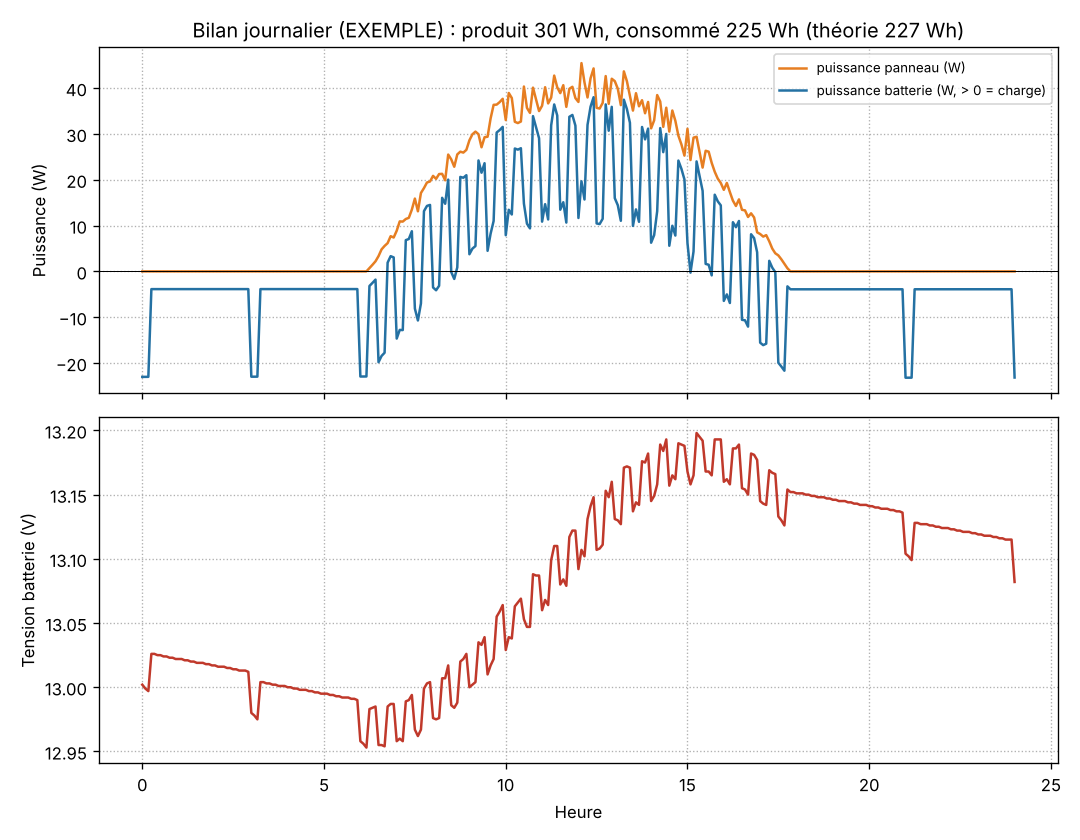
\includegraphics[width=0.9\textwidth]{img/elec/exemple_bilan_journee.png}
\caption{Sortie du script sur les données d'exemple : puissances du panneau et de la batterie, tension de la batterie.}
\end{figure}

\begin{figure}[H]
\centering
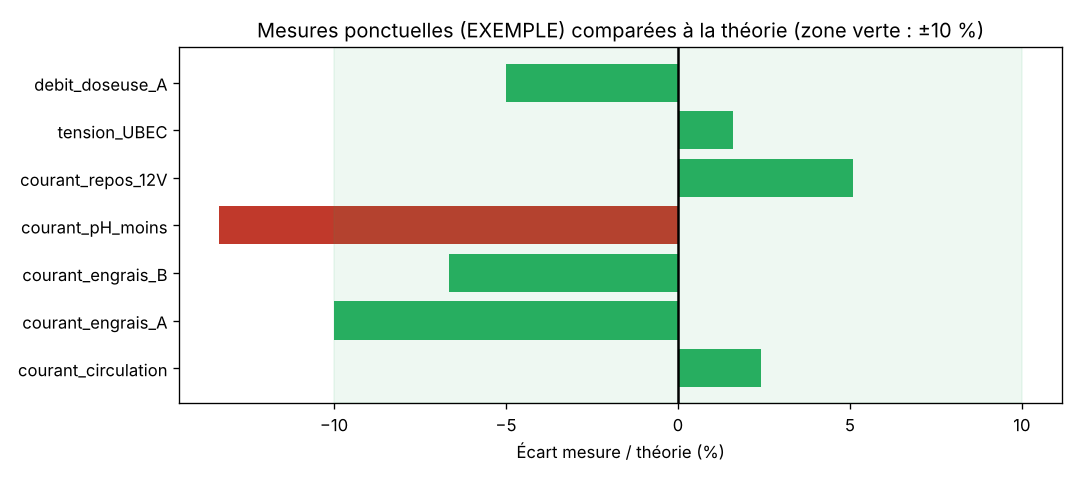
\includegraphics[width=0.85\textwidth]{img/elec/exemple_ecarts.png}
\caption{Sortie du script sur les données d'exemple : écart entre les mesures ponctuelles et la théorie.}
\end{figure}

\textbf{Exploitation.} Si un écart dépasse \qty{10}{\percent}, je remplace l'hypothèse correspondante par la valeur mesurée dans le calcul, je relance le calcul et je mets à jour le bilan de la partie 5.3. Les chiffres de cette partie sont calculés : aucune mesure réelle n'est encore faite.

\begin{aretenir}
Cinq séries de mesures : le courant de chaque pompe (M1), la consommation au repos et le rendement de l'UBEC\ix{17} (M2), le bilan d'une journée enregistré par l'INA260\ix{22} toutes les \qty{5}{min} (M3), les tensions et l'identification des batteries (M4), le débit des doseuses (M5). Le script intègre les puissances par la méthode des trapèzes, déduit la consommation réelle et la compare à la théorie ; il a été vérifié sur des données d'exemple.
\end{aretenir}

\Needspace{8\baselineskip}\subsection{Les hypothèses de l'étude}

Chaque hypothèse est à confirmer, par les mesures M1 à M5 du protocole ou par la lecture des étiquettes et des notices.

\textbf{Données reprises de la version 1.} Le TE1250 a une puissance crête de \qty{120}{Wc}, une puissance minimale de \qty{117,5}{W}, $V_{mp} = \qty{17,6}{V}$, $I_{mp} = \qty{6,8}{A}$, $I_{sc} = \qty{7,3}{A}$, $V_{oc} = \qty{22,0}{V}$ et un fusible série maximal de \qty{10}{A}. L'irradiation du pire mois n'est plus reprise de la version 1 : elle vient de Solargis (juin, $H = \qty{3,607}{kWh/m^2/j}$, partie 5.4). Le rendement du convertisseur \qty{12}{V} vers \qty{5}{V} est de $0{,}83$.

\textbf{Panneau.} Les coefficients de température du TE1250 sont pris égaux à ceux du SLP055 (même technologie à 36 cellules) : $V_{oc}$ de $-\qty{80}{mV/\celsius}$, $I_{sc}$ de $+\qty{0,065}{\percent/\celsius}$, $P_{\max}$ de $-\qty{0,5}{\percent/\celsius}$, NOCT de \qty{47}{\celsius}. Le TE1250 a 36 cellules en série (cohérent avec $V_{oc} = \qty{22}{V}$). Le calcul se fait directement sur le panneau entier, sans modèle de cellule. La température de l'air en milieu de journée du pire mois est de \qty{27}{\celsius}, et l'éclairement de calcul de la température de cellule de \qty{800}{W/m^2}, d'où $T_c = \qty{54}{\celsius}$. Les facteurs de pertes sont 0,95 (salissures, sel et orientation), 0,95 (régulateur MPPT\ix{19}), 0,98 (câbles) et 0,95 (LiFePO4) ou 0,85 (AGM) pour la batterie, appliqué à toute l'énergie (prudent). Un jour très couvert apporte \qty{1,2}{kWh/m^2/j}.

\textbf{Consommation.} Le Raspberry Pi 3 B sans écran, en charge faible, consomme \qty{450}{mA} en moyenne à \qty{5}{V} (plage typique de \qty{260}{mA} à \qty{500}{mA} au repos, plus en charge). Le dongle Wi-Fi USB à antenne externe consomme \qty{120}{mA} en moyenne (émission intermittente). L'Arduino Uno R3 consomme \qty{50}{mA}, les capteurs leurs courants de fiche typiques, et la sonde EC n'est alimentée que 2 secondes par minute environ. La pompe de circulation consomme \qty{19}{W} (\qty{1,48}{A} à \qty{12,8}{V}) avec un planning de \qty{6,75}{h/j}. Le MOSFET\ix{15} de la carte 6318 a $R_{DS(on)} = \qty{70}{m\ohm}$ par canal. Les pompes doseuses consomment \qty{0,30}{A} sous \qty{12}{V} et débitent \qty{80}{mL/min} en charge (la fiche annonce jusqu'à \qty{100}{mL/min} à vide). Pour le dosage, je suppose une baisse d'EC de \qty{0,05}{mS/cm} par jour dans \qty{152}{L}, une sensibilité de la solution mère de \qty{0,56}{mS/cm} pour \qty{1}{mL/L} de A et de B, et \qty{6}{mL/j} de pH$-$ ; l'énergie retenue est un majorant de 10 commandes de \qty{30}{s} par pompe et par jour (\qty{0,96}{Wh/j}). L'autoconsommation du régulateur est de \qty{15}{mA} à \qty{12,8}{V}. La nuit de calcul dure 14 h (de 17 h à 7 h), avec 7 marches de \qty{15}{min} de la circulation.

\textbf{Batteries.} Mes batteries sont au plomb (Yuasa NP17-12I au plomb étanche, Steco de type AGM à confirmer sur son étiquette), alors que le cahier des charges de départ parlait de LiFePO4 : les deux cas sont donc calculés, et le plomb AGM est retenu pour les conclusions. En LiFePO4 : \qty{12,8}{V}, DoD\ix{27} 80\,\%, rendement 0,95, charge admise $0{,}5\,C$, absorption de \qty{14,2}{V} à \qty{14,6}{V}. En AGM : \qty{12,0}{V}, DoD\ix{27} 50\,\%, rendement 0,85, charge conseillée $0{,}25\,C$, absorption de \qty{14,4}{V} à \qty{14,7}{V}. La résistance interne de la batterie de \qty{6}{Ah} est supposée de \qty{60}{m\ohm}, celle de la \qty{17}{Ah} se déduit par proportion inverse à la capacité (\qty{21}{m\ohm}). Le seuil de mode sobriété proposé est de \qty{12,9}{V} au repos (LiFePO4), à ajuster.

\textbf{Câbles et fusibles.} La résistivité du cuivre à \qty{60}{\celsius} est de \qty{0,0199}{\ohm.mm^2/m}. Les longueurs sont de \qty{5}{m} du panneau au régulateur, \qty{0,5}{m} du régulateur au bus, \qty{0,3}{m} du bus à chaque batterie, \qty{0,5}{m} de la sortie LOAD au bornier, \qty{3}{m} du bornier à la pompe de circulation, \qty{1}{m} vers les doseuses et \qty{0,3}{m} de l'UBEC\ix{17} au Pi. Les chutes admises sont de \qty{3}{\percent} côté panneau et pompes, \qty{1}{\percent} côté batterie, \qty{0,5}{\percent} entre batteries et \qty{2}{\percent} sur le \qty{5}{V}. Le régulateur est à positif commun d'après sa notice : $PV-$, $BAT-$ et $LOAD-$ sont trois bornes séparées, qu'il ne faut jamais relier entre elles. Sa tension d'entrée maximale, \qty{70}{V} d'après la fiche, est très supérieure aux \qty{22,4}{V} du panneau à froid.

\Needspace{8\baselineskip}\subsection{La synthèse de l'étude électrique}

Le tableau suivant résume les résultats de l'étude électrique.

\begin{table}[H]
\centering
\small
\begin{tabular}{|l|c|c|}
\hline
\textbf{Résultat} & \textbf{Version 1} & \textbf{Version 2} \\
\hline
Consommation journalière & \qty{281}{Wh/j} & \qty{226,7}{Wh/j} \\
\hline
Production théorique (\qty{120}{Wc}) & \qty{504}{Wh/j} ($H = 4{,}2$) & \qty{432,8}{Wh/j} ($H = \num{3,607}$, juin) \\
\hline
Production disponible le pire mois & \qty{336}{Wh/j} & \qty{304,5}{Wh/j} (LiFePO4) / \qty{272,4}{Wh/j} (AGM) \\
\hline
Marge du panneau & $+20\,\%$ & $+34\,\%$ (LiFePO4) / $+20\,\%$ (AGM) \\
\hline
Énergie utilisable des batteries (\qty{23}{Ah}) & & \qty{235,5}{Wh} (LiFePO4) / \qty{138,0}{Wh} (AGM) \\
\hline
Part de la nuit dans l'énergie utilisable & & 38\,\% (LiFePO4) / 65\,\% (AGM) \\
\hline
Autonomie sans soleil & & \qty{1,0}{j} (LiFePO4) / \qty{0,6}{j} (AGM) \\
\hline
Fusibles & 10 / 5 / 15 / \qty{7,5}{A} & 10 / 5 / 15 / \qty{4}{A} + \qty{2}{A} (UBEC\ix{17}) \\
\hline
\end{tabular}
\caption{Synthèse de l'étude électrique.}
\end{table}

\begin{aretenir}
Le panneau TE1250 de \qty{120}{Wc} couvre le besoin du pire mois, juin (\qty{272}{Wh/j} pour \qty{227}{Wh/j} en plomb AGM, soit $+20\,\%$). Les batteries de \qty{23}{Ah} couvrent la nuit sans difficulté, mais seulement un à deux jours très couverts en LiFePO4 (un seul en AGM) : un mode sobriété basé sur la tension de la batterie est à programmer. Points à vérifier en priorité : la technologie réelle des deux batteries (étiquette de la Steco), le réglage du régulateur et le câblage séparé de ses trois bornes négatives, le courant de charge maximal réglable, puis les mesures M1 à M5.
\end{aretenir}


% ===== ETUDE THERMIQUE =====
% =====================================================================
\clearpage
\partieENO{La thermodynamique}

Cette partie traite de la chaleur : à quelle température l'eau du bac va-t-elle se stabiliser, et que faire si elle est trop chaude ? La température de l'eau compte pour les racines : au-dessus d'environ \qty{26}{\celsius}, l'eau contient moins d'oxygène et les maladies des racines progressent. Je commence par le bilan de chaleur du bac (6.1). J'en déduis l'effet de la couleur (6.2), puis la chaleur ajoutée par la pompe (6.3). Je raffine ensuite le bilan avec l'évaporation et le rayonnement (6.4), puis je calcule les pertes par effet Joule de l'installation, à partir des données de l'étude électrique (6.5). Je regarde la chaleur reçue par la tour et les tuyaux (6.6), l'échauffement de l'armoire et de la batterie (6.7), et les solutions si l'eau est trop chaude (6.8). Je termine par ce que je mesurerai (6.9). Il n'y a encore aucune mesure : ce sont des calculs, à partir d'hypothèses signalées.

\Needspace{8\baselineskip}\subsection{Le bilan de chaleur du bac}

\subsubsection*{Ce que je cherche et ce que je suppose}

Je cherche de combien le soleil réchauffe l'eau du bac, et quelle température elle atteint. Le bac reçoit de la chaleur du soleil, en reçoit de la pompe, et en échange avec l'air. Je suppose un bac parallélépipédique de $\qty{0,70}{m} \times \qty{0,45}{m} \times \qty{0,48}{m}$ (volume intérieur proche de \qty{151}{L}, hypothèse à mesurer), un coefficient d'échange avec l'air $h = \qty{8}{W/(m^2\,K)}$ (air calme à peu agité, hypothèse), un éclairement de \qty{800}{W/m^2} sur le dessus à midi, et une irradiation de \qty{4,2}{kWh/m^2/j} (valeur de ma première étude électrique ; la moyenne annuelle de Solargis est de \qty{4,74}{kWh/m^2/j}, partie 5.4). La chaleur massique de l'eau est $c = \qty{4180}{J/(kg\,K)}$ et \qty{152}{L} d'eau pèsent \qty{152}{kg}.

\naturecalc{théorie (formule démontrée, valeurs de fiches techniques et hypothèses ; rien de mesuré)}
\begin{demonstration}[température du bac au cours du temps]
\resultat{\Delta T(t) = \Delta T_{\infty}\left(1 - e^{-t/\tau}\right)}
Je note $T$ la température de l'eau, en °C, $T_a$ celle de l'air, en °C, $\Delta T = T - T_a$ l'élévation, en kelvins, $m$ la masse d'eau, en kg, $c$ sa chaleur massique, en J/(kg$\cdot$K), $C = m\,c$ la capacité thermique, en J/K, $P_s$ la puissance solaire absorbée, en watts, $h$ le coefficient d'échange, en W/(m$^2\cdot$K), $S_t$ la surface totale d'échange du bac, en m$^2$. L'énergie gagnée par l'eau pendant $\mathrm{d}t$ est la puissance reçue moins la puissance perdue vers l'air :
\begin{align*}
C\,\frac{\mathrm{d}T}{\mathrm{d}t} &= P_s - h\,S_t\,(T - T_a)\\
\dimline{\unit{J/K}\times\unit{K/s}=\unit{J/s}=\unit{W}\ ;\ \unit{W/(m^2\,K)}\times\unit{m^2}\times\unit{K}=\unit{W}}
\end{align*}
Comme $T_a$ est constant, $\mathrm{d}T/\mathrm{d}t = \mathrm{d}(\Delta T)/\mathrm{d}t$. Je pose $G_t = h\,S_t$ (en W/K) :
\begin{align*}
C\,\frac{\mathrm{d}(\Delta T)}{\mathrm{d}t} + G_t\,\Delta T &= P_s
\end{align*}
Je divise par $G_t$ et je pose $\tau = C/G_t$ (en secondes) et $\Delta T_{\infty} = P_s/G_t$ :
\begin{align*}
\tau\,\frac{\mathrm{d}(\Delta T)}{\mathrm{d}t} + \Delta T &= \Delta T_{\infty}
\end{align*}
Je sépare les variables : $\dfrac{\mathrm{d}(\Delta T)}{\Delta T_{\infty} - \Delta T} = \dfrac{\mathrm{d}t}{\tau}$. J'intègre de $0$ (où $\Delta T = 0$) à $t$ :
\begin{align*}
-\ln\!\left(\Delta T_{\infty} - \Delta T\right) \Big|_{0}^{t} &= \frac{t}{\tau}\\
\ln\frac{\Delta T_{\infty}}{\Delta T_{\infty} - \Delta T(t)} &= \frac{t}{\tau}\\
\Delta T(t) &= \Delta T_{\infty}\left(1 - e^{-t/\tau}\right)
\end{align*}
L'eau tend donc vers $\Delta T_{\infty}$ avec la constante de temps $\tau$.
\end{demonstration}

\naturecalc{théorie (formule démontrée, valeurs de fiches techniques et hypothèses ; rien de mesuré)}
\begin{demonstration}[capacité thermique, surface et constante de temps]
\resultat{\tau \approx \qty{12,7}{h}}
\begin{align*}
C &= m\,c = \qty{152}{kg} \times \qty{4180}{J/(kg\,K)} \approx \qty{635360}{J/K}\\
\dimline{\unit{kg}\times\unit{J/(kg\,K)}=\unit{J/K}}
\end{align*}
La surface totale d'échange est celle des six faces du bac, deux fois la somme des trois produits de côtés :
\begin{align*}
S_t &= 2\,(L\,l + L\,H_b + l\,H_b)\\
S_t &= 2\,(\qty{0,70}{m}\times\qty{0,45}{m} + \qty{0,70}{m}\times\qty{0,48}{m} + \qty{0,45}{m}\times\qty{0,48}{m})\\
S_t &= 2\,(\qty{0,315}{m^2} + \qty{0,336}{m^2} + \qty{0,216}{m^2})\\
S_t &\approx \qty{1,734}{m^2}\\
\dimline{\unit{m}\times\unit{m}=\unit{m^2}}
\end{align*}
\begin{align*}
G_t &= h\,S_t = \qty{8}{W/(m^2\,K)} \times \qty{1,734}{m^2} \approx \qty{13,87}{W/K}\\
\dimline{\unit{W/(m^2\,K)}\times\unit{m^2}=\unit{W/K}}\\
\tau &= \frac{C}{G_t} = \frac{\qty{635360}{J/K}}{\qty{13,87}{W/K}} \approx \qty{45800}{s} \approx \qty{12,7}{h}\\
\dimline{\dfrac{\unit{J/K}}{\unit{W/K}}=\dfrac{\unit{J}}{\unit{J/s}}=\unit{s}}
\end{align*}
Le bac a une grande inertie : il met environ 13 heures à rattraper 63\,\% de l'écart. Il lisse donc les variations de la journée.
\end{demonstration}

\textbf{Limite sur la surface d'échange.} J'ai compté les six faces du bac comme échangeant avec l'air. Si le fond repose sur un support ou sur le sol, il échange beaucoup moins. Sans le fond (\qty{0,315}{m^2}), la surface vaut $\qty{1,734}{m^2} - \qty{0,315}{m^2} = \qty{1,419}{m^2}$, donc $G_t = \qty{8}{W/(m^2\,K)} \times \qty{1,419}{m^2} \approx \qty{11,35}{W/K}$ et $\tau \approx \qty{15,5}{h}$. Les élévations de température calculées plus bas seraient alors environ 22 \% plus grandes. Mon modèle est donc plutôt prudent sur ce point, et la mesure de $\tau$ du protocole permettra de choisir la bonne surface.

\Needspace{8\baselineskip}\subsection{Pourquoi le bac est peint en blanc}

Une surface absorbe une part $\alpha$ de la lumière du soleil. Pour une surface noire, $\alpha$ est d'environ $0{,}9$ ; pour une surface blanche, environ $0{,}25$ (valeurs usuelles pour les peintures, hypothèses). La puissance absorbée par le dessus du bac, de surface $S_{top} = L\,l = \qty{0,315}{m^2}$ sous $G = \qty{800}{W/m^2}$, vaut $P_s = \alpha\,G\,S_{top}$.

\naturecalc{théorie (formule démontrée, valeurs de fiches techniques et hypothèses ; rien de mesuré)}
\begin{demonstration}[effet de la couleur sur l'élévation de température]
\resultat{\Delta T_{\infty} = \dfrac{\alpha\,G\,S_{top}}{h\,S_t}}
Je reprends $\Delta T_{\infty} = P_s/G_t$ avec $P_s = \alpha\,G\,S_{top}$ et $G_t = \qty{13,87}{W/K}$ :
\begin{align*}
P_{s,noir} &= 0{,}9 \times \qty{800}{W/m^2} \times \qty{0,315}{m^2} = \qty{226,8}{W}\\
P_{s,blanc} &= 0{,}25 \times \qty{800}{W/m^2} \times \qty{0,315}{m^2} = \qty{63,0}{W}\\
\dimline{\unit{W/m^2}\times\unit{m^2}=\unit{W}}
\end{align*}
\begin{align*}
\Delta T_{\infty,noir} &= \frac{\qty{226,8}{W}}{\qty{13,87}{W/K}} \approx \qty{16,3}{K}\\
\Delta T_{\infty,blanc} &= \frac{\qty{63,0}{W}}{\qty{13,87}{W/K}} \approx \qty{4,5}{K}\\
\dimline{\dfrac{\unit{W}}{\unit{W/K}}=\unit{K}}
\end{align*}
Sur les six premières heures de soleil ($t = \qty{21600}{s}$), le facteur $1 - e^{-t/\tau}$ vaut :
\begin{align*}
1 - e^{-21600/45800} &= 1 - e^{-0{,}472} \approx 0{,}376\\
\dimline{\dfrac{\unit{s}}{\unit{s}}=\text{sans unité}}
\end{align*}
\begin{align*}
\Delta T_{noir}(\qty{6}{h}) &= \qty{16,3}{K} \times 0{,}376 \approx \qty{6,1}{K}\\
\Delta T_{blanc}(\qty{6}{h}) &= \qty{4,5}{K} \times 0{,}376 \approx \qty{1,7}{K}\\
\dimline{\text{sans unité}\times\unit{K}=\unit{K}}
\end{align*}
\end{demonstration}

La figure suivante montre comment la température de l'eau du bac monte au cours d'une journée de soleil, selon la couleur du bac.

\begin{figure}[H]
\centering
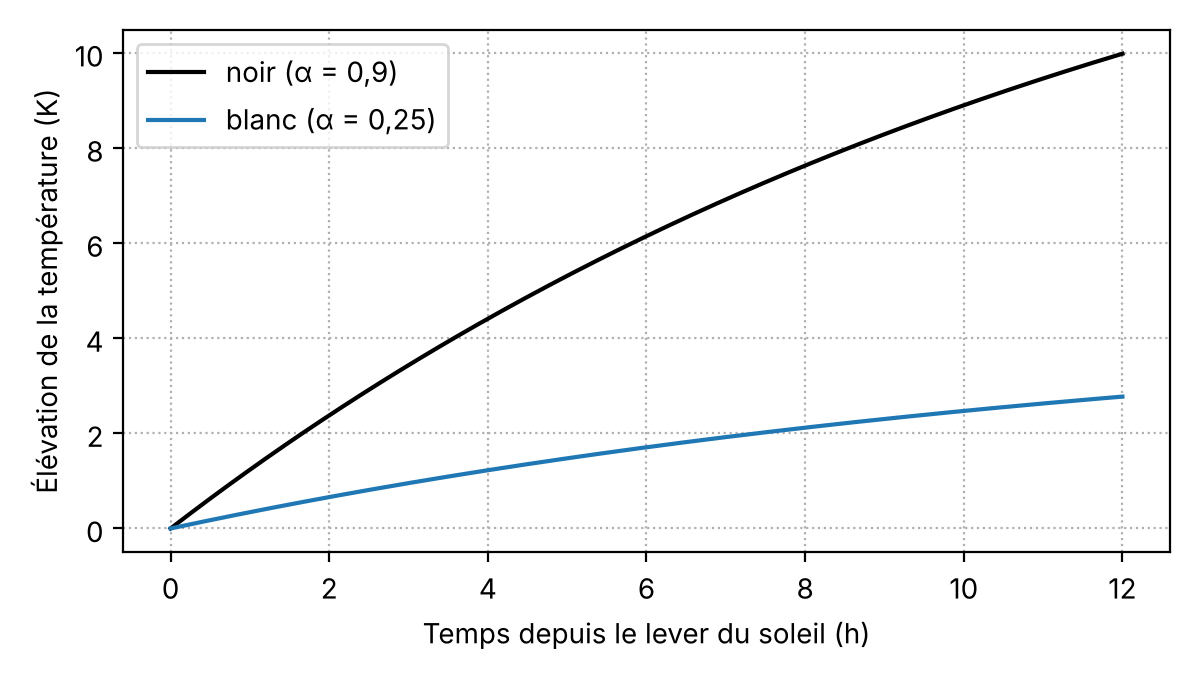
\includegraphics[width=0.72\textwidth]{img/thermo.png}
\caption{Élévation de la température de l'eau du bac au cours d'une journée de soleil, selon la couleur du bac (calcul).}
\end{figure}

Le blanc évite donc environ \qty{4,4}{K} d'échauffement en six heures de plein soleil. Pour la journée entière, avec l'irradiation de \qty{4,2}{kWh/m^2/j} retenue dans ma première étude électrique (soit une puissance moyenne $H/24\,\mathrm{h} = \qty{175}{W/m^2}$), l'élévation moyenne est :

\naturecalc{théorie (formule démontrée, valeurs de fiches techniques et hypothèses ; rien de mesuré)}
\begin{demonstration}[élévation moyenne sur 24 heures]
\resultat{\overline{\Delta T} = \dfrac{\alpha\,H\,S_{top}}{\qty{24}{h}\; h\,S_t}}
La chaleur absorbée sur un jour vaut $\alpha\,H\,S_{top}$ et la chaleur évacuée par kelvin et par jour vaut $24\,h\,G_t$. Analyse dimensionnelle : $\unit{Wh/m^2}\times\unit{m^2}=\unit{Wh}$ et $\unit{h}\times\unit{W/K}=\unit{Wh/K}$. En noir, $0{,}9 \times \qty{4200}{Wh/m^2} \times \qty{0,315}{m^2} = \qty{1190,7}{Wh}$ par jour, et $\qty{24}{h} \times \qty{13,87}{W/K} = \qty{332,9}{Wh/K}$ :
\begin{align*}
\overline{\Delta T}_{noir} &= \frac{\qty{1190,7}{Wh}}{\qty{332,9}{Wh/K}} \approx \qty{3,6}{K}\\
\overline{\Delta T}_{blanc} &= \frac{0{,}25 \times \qty{4200}{Wh} \times 0{,}315}{\qty{332,9}{Wh/K}} = \frac{\qty{330,8}{Wh}}{\qty{332,9}{Wh/K}} \approx \qty{1,0}{K}\\
\dimline{\dfrac{\unit{Wh}}{\unit{Wh/K}}=\unit{K}}
\end{align*}
\end{demonstration}

\Needspace{8\baselineskip}\subsection{La chaleur ajoutée par la pompe}

La pompe est immergée : toute la puissance électrique qui ne sert pas à monter l'eau finit en chaleur dans le bac. La puissance hydraulique est $P_h = \rho\,g\,Q\,H$.

\naturecalc{théorie (formule démontrée, valeurs de fiches techniques et hypothèses ; rien de mesuré)}
\begin{demonstration}[chaleur dégagée par la pompe]
\resultat{\overline{\Delta T}_{pompe} \approx \qty{0,33}{K}}
Je note $\rho = \qty{997}{kg/m^3}$ la masse volumique de l'eau, $g = \qty{9,81}{m/s^2}$, $Q$ le débit en m$^3$/s et $H$ la hauteur manométrique en mètres. La puissance hydraulique est l'énergie potentielle gagnée par seconde par l'eau montée :
\begin{align*}
P_h &= \rho\,g\,Q\,H
\end{align*}
Avec $Q = \qty{388}{L/h} = \qty{1,078e-4}{m^3/s}$ et $H = \qty{2,57}{m} $ (partie 3) :
\begin{align*}
P_h &= \qty{997}{kg/m^3} \times \qty{9,81}{m/s^2} \times \qty{1,078e-4}{m^3/s} \times \qty{2,57}{m}\\
P_h &\approx \qty{2,7}{W}\\
\dimline{\unit{kg/m^3}\times\unit{m/s^2}\times\unit{m^3/s}\times\unit{m}=\unit{kg\,m^2/s^3}=\unit{W}}
\end{align*}
La chaleur dégagée par la pompe en marche est le reste de ses \qty{19}{W} :
\begin{align*}
P_{q} &= \qty{19}{W} - \qty{2,7}{W} = \qty{16,3}{W}\\
\dimline{\unit{W}-\unit{W}=\unit{W}}
\end{align*}
Elle ne marche que \qty{6,75}{h} par jour. La puissance moyenne et l'élévation moyenne de température associée valent :
\begin{align*}
\overline{P}_q &= \qty{16,3}{W} \times \frac{\qty{6,75}{h}}{\qty{24}{h}} \approx \qty{4,6}{W}\\
\overline{\Delta T}_{pompe} &= \frac{\overline{P}_q}{G_t} = \frac{\qty{4,6}{W}}{\qty{13,87}{W/K}} \approx \qty{0,33}{K}\\
\dimline{\unit{W}\times\dfrac{\unit{h}}{\unit{h}}=\unit{W}\ ;\ \dfrac{\unit{W}}{\unit{W/K}}=\unit{K}}
\end{align*}
\end{demonstration}


\textbf{Où va l'énergie hydraulique.} Je retire les \qty{2,7}{W} de puissance hydraulique de la chaleur de la pompe parce qu'ils servent à monter l'eau. Mais l'eau redescend dans le bac par ruissellement et cette énergie est dissipée par les frottements et les turbulences, en grande partie dans l'eau du circuit qui retourne au bac. Le cas le plus défavorable est donc que les \qty{19}{W} entiers chauffent le bac : $\overline{\Delta T}_{pompe} = \qty{19}{W} \times (\qty{6,75}{h}/\qty{24}{h}) / \qty{13,87}{W/K} \approx \qty{0,385}{K}$, soit \qty{0,05}{K} de plus que la valeur retenue. La différence est faible, mais elle va dans le sens d'une eau un peu plus chaude.

\Needspace{8\baselineskip}\subsection{L'évaporation et le rayonnement}

Le bilan du début regroupe tous les échanges avec l'air dans un seul coefficient $h$. Je sépare ici deux effets qui changent la température de l'eau : le rayonnement vers le ciel et l'évaporation. Je vérifie d'abord que la valeur $h = \qty{8}{W/(m^2\,K)}$ est cohérente, puis j'ajoute les deux effets au bilan.

\naturecalc{théorie (formule démontrée, valeurs de fiches techniques et hypothèses ; rien de mesuré)}
\begin{demonstration}[coefficient d'échange par rayonnement]
\resultat{h_r = 4\,\varepsilon\,\sigma\,T_m^3 \approx \qty{5,5}{W/(m^2\,K)}}
Je note $\varepsilon$ l'émissivité de la surface (sans unité), $\sigma = \qty{5,67e-8}{W/(m^2\,K^4)}$ la constante de Stefan-Boltzmann, $T_s$ la température absolue de la surface et $T_a$ celle de l'air, en kelvins, et $S$ l'aire de la surface, en m$^2$. La puissance nette rayonnée par la surface vers l'air vaut :
\begin{align*}
P_r &= \varepsilon\,\sigma\,S\,\left(T_s^4 - T_a^4\right)\\
\dimline{\unit{W/(m^2\,K^4)}\times\unit{m^2}\times\unit{K^4}=\unit{W}}
\end{align*}
Je factorise la différence de deux puissances quatrièmes en deux étapes :
\begin{align*}
T_s^4 - T_a^4 &= \left(T_s^2 - T_a^2\right)\left(T_s^2 + T_a^2\right)\\
T_s^4 - T_a^4 &= \left(T_s - T_a\right)\left(T_s + T_a\right)\left(T_s^2 + T_a^2\right)
\end{align*}
Quand $T_s$ et $T_a$ sont proches d'une température moyenne $T_m$, on a $T_s + T_a \approx 2\,T_m$ et $T_s^2 + T_a^2 \approx 2\,T_m^2$ :
\begin{align*}
T_s^4 - T_a^4 &\approx \left(T_s - T_a\right) \times 2\,T_m \times 2\,T_m^2\\
T_s^4 - T_a^4 &\approx 4\,T_m^3\,\left(T_s - T_a\right)
\end{align*}
La puissance devient proportionnelle à l'écart de température, comme un échange par convection :
\begin{align*}
P_r &= \underbrace{4\,\varepsilon\,\sigma\,T_m^3}_{h_r}\; S\,\left(T_s - T_a\right)
\end{align*}
Avec $\varepsilon = 0{,}9$ (peinture, hypothèse) et $T_m = \qty{300}{K}$ :
\begin{align*}
h_r &= 4 \times 0{,}9 \times \qty{5,67e-8}{W/(m^2\,K^4)} \times (\qty{300}{K})^3\\
h_r &= 4 \times 0{,}9 \times \qty{5,67e-8}{W/(m^2\,K^4)} \times \qty{2,7e7}{K^3}\\
h_r &\approx \qty{5,51}{W/(m^2\,K)}\\
\dimline{\unit{W/(m^2\,K^4)}\times\unit{K^3}=\unit{W/(m^2\,K)}}
\end{align*}
Le coefficient total est la somme de la convection $h_c$ et du rayonnement $h_r$. Avec $h = \qty{8}{W/(m^2\,K)}$ :
\begin{align*}
h_c &= h - h_r = \qty{8}{W/(m^2\,K)} - \qty{5,51}{W/(m^2\,K)}\\
h_c &\approx \qty{2,5}{W/(m^2\,K)}\\
\dimline{\unit{W/(m^2\,K)}-\unit{W/(m^2\,K)}=\unit{W/(m^2\,K)}}
\end{align*}
Une convection de \qty{2,5}{W/(m^2\,K)} correspond à un air presque calme : la valeur $h = \qty{8}{W/(m^2\,K)}$ est donc plausible, et même plutôt prudente quand il y a du vent.
\end{demonstration}

Le rayonnement a un second effet que $h$ ne contient pas. Le dessus du bac ne voit pas que l'air : il voit aussi le ciel, dont la température équivalente est plus basse que celle de l'air. Il perd donc de la chaleur en plus.

\naturecalc{théorie (formule démontrée, valeurs de fiches techniques et hypothèses ; rien de mesuré)}
\begin{demonstration}[refroidissement par le ciel]
\resultat{\Delta T_{ciel} \approx \qty{0,6}{K}}
Je note $T_c$ la température équivalente du ciel, en kelvins. Je suppose $T_a = \qty{300}{K}$ et un ciel plus froid de $\qty{10}{K}$, soit $T_c = \qty{290}{K}$ (hypothèse pour un air tropical humide). La puissance supplémentaire perdue par le dessus du bac, de surface $S_{top} = \qty{0,315}{m^2}$, est la puissance rayonnée vers le ciel moins celle déjà comptée vers l'air, soit :
\begin{align*}
P_{ciel} &= \varepsilon\,\sigma\,S_{top}\,\left(T_a^4 - T_c^4\right)
\end{align*}
\begin{align*}
T_a^4 &= (\qty{300}{K})^4 = \qty{8,100e9}{K^4}\\
T_c^4 &= (\qty{290}{K})^4 = \qty{7,073e9}{K^4}\\
T_a^4 - T_c^4 &= \qty{1,027e9}{K^4}\\
\dimline{\unit{K}^4=\unit{K^4}}
\end{align*}
\begin{align*}
P_{ciel} &= 0{,}9 \times \qty{5,67e-8}{W/(m^2\,K^4)} \times \qty{0,315}{m^2} \times \qty{1,027e9}{K^4}\\
P_{ciel} &\approx \qty{16,5}{W}\\
\dimline{\unit{W/(m^2\,K^4)}\times\unit{m^2}\times\unit{K^4}=\unit{W}}
\end{align*}
Cette perte n'existe que par ciel dégagé. Je suppose qu'il l'est la moitié du temps. L'abaissement moyen de la température d'équilibre est la puissance moyenne divisée par $G_t = \qty{13,87}{W/K}$ :
\begin{align*}
\Delta T_{ciel} &= \frac{0{,}5 \times \qty{16,5}{W}}{\qty{13,87}{W/K}}\\
\Delta T_{ciel} &\approx \qty{0,6}{K}\\
\dimline{\dfrac{\unit{W}}{\unit{W/K}}=\unit{K}}
\end{align*}
\end{demonstration}

Le troisième effet est l'évaporation. Le bac est fermé par son couvercle, mais l'eau qui monte dans la tour mouille les paniers et les racines, et les plants transpirent. L'eau qui part en vapeur emporte de la chaleur, et une partie de cette chaleur est prise à l'eau qui circule.

\naturecalc{théorie (formule démontrée, valeurs de fiches techniques et hypothèses ; rien de mesuré)}
\begin{demonstration}[refroidissement par l'évaporation]
\resultat{\Delta T_{evap} \approx \qty{0,9}{K}\ \text{(consommation moyenne)}}
Je note $m_{ev}$ la masse d'eau qui part en vapeur par jour, en kg/j, $L_v = \qty{2,43e6}{J/kg}$ la chaleur latente de vaporisation de l'eau vers \qty{30}{\celsius} (valeur usuelle, à valider), et $\varphi$ la part de cette chaleur prise à l'eau du bac (sans unité). Par définition de la chaleur latente, l'énergie qu'il faut pour évaporer la masse $m_{ev}$ vaut :
\begin{align*}
Q_{ev} &= m_{ev}\,L_v\\
\dimline{\unit{kg}\times\unit{J/kg}=\unit{J}}
\end{align*}
L'eau consommée par la tour part en vapeur (partie 3.5). Avec la consommation moyenne $m_{ev} = \qty{2,3}{kg/j}$ (\qty{2,3}{L/j}) :
\begin{align*}
Q_{ev} &= \qty{2,3}{kg/j} \times \qty{2,43e6}{J/kg}\\
Q_{ev} &\approx \qty{5,59e6}{J/j}\\
\dimline{\unit{kg/j}\times\unit{J/kg}=\unit{J/j}}
\end{align*}
La puissance moyenne correspondante est cette énergie divisée par la durée d'un jour, \qty{86400}{s} :
\begin{align*}
\overline{P}_{ev} &= \frac{\qty{5,59e6}{J/j}}{\qty{86400}{s/j}}\\
\overline{P}_{ev} &\approx \qty{64,7}{W}\\
\dimline{\dfrac{\unit{J/j}}{\unit{s/j}}=\dfrac{\unit{J}}{\unit{s}}=\unit{W}}
\end{align*}
Je suppose $\varphi = 0{,}2$ : le reste de la chaleur est pris à l'air et aux feuilles (hypothèse, à mesurer). L'abaissement de la température d'équilibre vaut :
\begin{align*}
\Delta T_{evap} &= \frac{\varphi\,\overline{P}_{ev}}{G_t} = \frac{0{,}2 \times \qty{64,7}{W}}{\qty{13,87}{W/K}}\\
\Delta T_{evap} &\approx \qty{0,93}{K}\\
\dimline{\dfrac{\unit{W}}{\unit{W/K}}=\unit{K}}
\end{align*}
Avec la consommation de pointe $m_{ev} = \qty{4,1}{kg/j}$, le même calcul donne $\overline{P}_{ev} \approx \qty{115,3}{W}$ et $\Delta T_{evap} \approx \qty{1,7}{K}$.
\end{demonstration}

Je regroupe maintenant tous les effets pour l'élévation moyenne de l'eau au-dessus de l'air.

\naturecalc{théorie (formule démontrée, valeurs de fiches techniques et hypothèses ; rien de mesuré)}
\begin{demonstration}[bilan moyen de la température du bac]
\resultat{\overline{\Delta T} = \Delta T_{soleil} + \Delta T_{pompe} - \Delta T_{ciel} - \Delta T_{evap} \approx \qty{-0,2}{K}}
Les effets s'additionnent, car le bilan de chaleur est linéaire : chaque puissance divisée par $G_t$ donne son effet sur l'écart d'équilibre. Avec le bac blanc (calculs précédents) :
\begin{align*}
\overline{\Delta T} &= \qty{1,0}{K} + \qty{0,33}{K} - \qty{0,6}{K} - \qty{0,93}{K}\\
\overline{\Delta T} &\approx \qty{-0,2}{K}\\
\dimline{\unit{K}+\unit{K}-\unit{K}-\unit{K}=\unit{K}}
\end{align*}
Avec la consommation de pointe, $\overline{\Delta T} = \qty{1,0}{K} + \qty{0,33}{K} - \qty{0,6}{K} - \qty{1,66}{K} \approx \qty{-0,9}{K}$ (\qty{1,66}{K} est la valeur non arrondie de l'effet de l'évaporation en pointe, arrondie à \qty{1,7}{K} plus haut).
\end{demonstration}

L'eau reste donc un peu sous la température moyenne de l'air, de \qtyrange{0,2}{0,9}{K}. Avec un air autour de \qty{27}{\celsius}, elle sera vers \qty{26}{\celsius} à \qty{27}{\celsius}. C'est mieux que les \qty{28}{\celsius} annoncés plus haut, mais cela reste au-dessus de la plage idéale de la laitue. Ces valeurs reposent sur des hypothèses ($\varepsilon$, $T_c$, $\varphi$) que le protocole de mesure doit confirmer.

\Needspace{8\baselineskip}\subsection{Les pertes par effet Joule de l'installation}

Toute l'énergie électrique consommée finit en chaleur, et les composants perdent en plus une part de ce qui les traverse. Je calcule ici les pertes par effet Joule dans les câbles, avec les longueurs, les courants et les sections de l'étude électrique (partie 5.7), puis je dresse la liste de toutes les sources de chaleur et de l'endroit où elles chauffent.

\naturecalc{théorie (formule démontrée, valeurs de fiches techniques et hypothèses ; rien de mesuré)}
\begin{demonstration}[perte Joule d'un câble et énergie perdue par jour]
\resultat{P_J = R\,I^2 = \dfrac{2\,\rho\,L\,I^2}{S} \qquad E_J = P_J\,t}
Je note $R$ la résistance du câble, en ohms, $I$ le courant, en ampères, $\rho$ la résistivité du cuivre, en $\unit{\ohm\,mm^2/m}$, $L$ la longueur de la liaison, en mètres, $S$ la section, en mm$^2$, et $t$ la durée pendant laquelle le courant passe, en heures. Le courant fait l'aller et le retour, donc la longueur de cuivre est $2L$ :
\begin{align*}
R &= \rho\,\frac{2\,L}{S}
\end{align*}
La loi d'Ohm donne la chute de tension $\Delta U = R\,I$ aux bornes du câble. La puissance perdue est le produit de cette chute par le courant :
\begin{align*}
P_J &= \Delta U \times I\\
P_J &= R\,I \times I\\
P_J &= R\,I^2 = \frac{2\,\rho\,L\,I^2}{S}\\
\dimline{\unit{\ohm}\times\unit{A^2}=\unit{V\,A}=\unit{W}}
\end{align*}
L'énergie perdue sur une journée est la puissance multipliée par la durée de passage du courant :
\begin{align*}
E_J &= P_J\,t\\
\dimline{\unit{W}\times\unit{h}=\unit{Wh}}
\end{align*}
\end{demonstration}

\naturecalc{théorie (formule démontrée, valeurs de fiches techniques et hypothèses ; rien de mesuré)}
\begin{demonstration}[perte Joule du câble panneau vers régulateur]
\resultat{E_J \approx \qty{9,7}{Wh/j}\ \text{(majorant)}}
Avec $\rho = \qty{0,0199}{\ohm\,mm^2/m}$ (cuivre à \qty{60}{\celsius}), $L = \qty{5}{m}$, $S = \qty{4}{mm^2}$ et $I = \qty{6,83}{A}$ :
\begin{align*}
R &= \frac{2 \times \qty{0,0199}{\ohm\,mm^2/m} \times \qty{5}{m}}{\qty{4}{mm^2}}\\
R &\approx \qty{0,0498}{\ohm}\\
\dimline{\dfrac{\unit{\ohm\,mm^2/m}\times\unit{m}}{\unit{mm^2}}=\unit{\ohm}}
\end{align*}
\begin{align*}
P_J &= \qty{0,0498}{\ohm} \times (\qty{6,83}{A})^2\\
P_J &\approx \qty{2,32}{W}\\
\dimline{\unit{\ohm}\times\unit{A^2}=\unit{V\,A}=\unit{W}}
\end{align*}
Le courant du panneau est proportionnel à l'éclairement $G$ : $I(t) = I_{mpp}\,G(t)/G_{STC}$. L'énergie perdue est donc $R\,I_{mpp}^2\int (G/G_{STC})^2\,\mathrm{d}t$. Comme $G \leq G_{STC}$ la plupart du temps, $(G/G_{STC})^2 \leq G/G_{STC}$, et l'intégrale est au plus égale aux heures équivalentes de plein soleil $H/G_{STC} = \qty{4,2}{h/j}$. J'obtiens un majorant :
\begin{align*}
E_J &\leq \qty{2,32}{W} \times \qty{4,2}{h/j}\\
E_J &\approx \qty{9,7}{Wh/j}\\
\dimline{\unit{W}\times\unit{h/j}=\unit{Wh/j}}
\end{align*}
\end{demonstration}

Les autres liaisons se calculent de la même façon. Pour les liaisons de charge des batteries, je prends aussi \qty{4,2}{h/j} (majorant), pour les liaisons de la pompe de circulation \qty{6,75}{h/j} (durée de marche), pour la doseuse \qty{0,25}{h/j} et pour l'alimentation du Pi \qty{24}{h/j}.

Le tableau suivant donne les pertes Joule de chaque liaison, en valeur majorante.

\begin{table}[H]
\centering
\small
\begin{tabular}{|l|c|c|c|c|c|c|}
\hline
\textbf{Liaison} & \textbf{$S$ (mm$^2$)} & \textbf{$R$ (m$\Omega$)} & \textbf{$I$ (A)} & \textbf{$P_J$ (W)} & \textbf{$t$ (h/j)} & \textbf{$E_J$ (Wh/j)} \\
\hline
Panneau vers MPPT\ix{19} & 4 & 49,8 & 6,83 & 2,32 & 4,2 & 9,75 \\
\hline
MPPT\ix{19} vers bus & 4 & 5,0 & 8,91 & 0,40 & 4,2 & 1,66 \\
\hline
Bus vers B1 & 2,5 & 4,8 & 2,32 & 0,03 & 4,2 & 0,11 \\
\hline
Bus vers B2 & 2,5 & 4,8 & 6,58 & 0,21 & 4,2 & 0,87 \\
\hline
Sortie LOAD vers bornier & 1,5 & 13,3 & 2,70 & 0,10 & 6,75 & 0,65 \\
\hline
Bornier vers circulation & 1,5 & 79,6 & 1,48 & 0,17 & 6,75 & 1,18 \\
\hline
Bornier vers doseuse & 0,5 & 79,6 & 0,30 & 0,01 & 0,25 & 0,00 \\
\hline
UBEC\ix{17} vers Pi (\qty{5}{V}) & 0,5 & 23,9 & 1,00 & 0,02 & 24 & 0,57 \\
\hline
\textbf{Total} & & & & & & \textbf{14,8} \\
\hline
\end{tabular}
\caption{Pertes Joule des câbles (majorants) : $R = 2\rho L/S$ avec $\rho = \qty{0,0199}{\ohm\,mm^2/m}$, longueurs et courants du tableau des sections de câbles.}
\end{table}

Les câbles perdent donc au plus \qty{14,8}{Wh/j}, soit $\qty{14,8}{Wh/j}/\qty{226,7}{Wh/j} \approx 6{,}5\,\%$ du besoin journalier. C'est un majorant : les liaisons côté panneau et batteries ne voient le courant maximal que quelques heures. La perte du câble du panneau, la plus grosse, est du même ordre que les $2\,\%$ de pertes de câbles ($k_{câbles} = 0{,}98$) déjà retenus dans l'énergie produite, soit environ \qty{8}{Wh/j} : le calcul confirme ce facteur.

\naturecalc{théorie (formule démontrée, valeurs de fiches techniques et hypothèses ; rien de mesuré)}
\begin{demonstration}[chaleur dégagée par le régulateur MPPT\ix{19}]
\resultat{P_{MPPT\ix{19}} \approx \qty{5,0}{W}\ \text{au plus (plein soleil)}}
Le facteur $k_{MPPT} = 0{,}95$ de l'étude électrique veut dire que le régulateur transmet au plus $95\,\%$ de la puissance reçue. Je note $P_{in}$ la puissance reçue du panneau, en watts, et $P_{out}$ la puissance rendue aux batteries. Le reste est de la chaleur :
\begin{align*}
P_{out} &= k_{MPPT}\,P_{in}\\
P_{MPPT} &= P_{in} - P_{out} = \left(1 - k_{MPPT}\right)P_{in}
\end{align*}
Au plein soleil, avec des cellules à \qty{54}{\celsius}, le panneau fournit $P_{max} = \qty{102,6}{W}$ (partie 5.4), réduits de $2\,\%$ par les câbles :
\begin{align*}
P_{in} &= 0{,}98 \times \qty{102,6}{W} \approx \qty{100,5}{W}\\
P_{MPPT} &= (1 - 0{,}95) \times \qty{100,5}{W}\\
P_{MPPT} &\approx \qty{5,0}{W}\\
\dimline{\text{sans unité}\times\unit{W}=\unit{W}}
\end{align*}
Sur une journée, l'énergie reçue vaut $\qty{504}{Wh/j} \times 0{,}855 \times 0{,}979 \times 0{,}95 \times 0{,}98 \approx \qty{392,8}{Wh/j}$ :
\begin{align*}
E_{MPPT} &= 0{,}05 \times \qty{392,8}{Wh/j}\\
E_{MPPT} &\approx \qty{19,6}{Wh/j}\\
\dimline{\text{sans unité}\times\unit{Wh/j}=\unit{Wh/j}}
\end{align*}
\end{demonstration}

Je regroupe toutes les sources de chaleur de l'installation. La pompe est immergée : sa chaleur va dans l'eau (calcul précédent, $\qty{16,3}{W} \times \qty{6,75}{h/j} \approx \qty{110,0}{Wh/j}$). Le reste chauffe l'armoire ou les câbles.

\begin{table}[H]
\centering
\small
\begin{tabular}{|l|c|r|}
\hline
\textbf{Source de chaleur} & \textbf{Où} & \textbf{$E$ (Wh/j)} \\
\hline
Électronique \qty{5}{V} ($\qty{3,175}{W} \times \qty{24}{h}$) & armoire & 76,2 \\
\hline
Pertes de l'UBEC\ix{17} & armoire & 15,6 \\
\hline
Pertes du MPPT\ix{19} (conversion) & armoire & 19,6 \\
\hline
Autoconsommation du MPPT\ix{19} & armoire & 4,6 \\
\hline
Pertes des MOSFET\ix{15} & armoire & 0,5 \\
\hline
\textbf{Total armoire} & & \textbf{116,5} \\
\hline
Pertes Joule des câbles (majorant) & câbles, air & 14,8 \\
\hline
Pompe de circulation (chaleur) & eau du bac & 110,0 \\
\hline
\end{tabular}
\caption{Où va la chaleur de l'installation.}
\end{table}

L'armoire reçoit en moyenne $\qty{116,5}{Wh/j}/\qty{24}{h} \approx \qty{4,9}{W}$. Les câbles perdent de la chaleur dans l'air, sans effet sur l'eau.

\Needspace{8\baselineskip}\subsection{La tour et les tuyaux au soleil}

Le bilan du bac ne compte que le dessus du bac. Or l'eau passe aussi dans la tour (tube blanc de \qty{159}{mm} de diamètre et \qty{1}{m} de haut) et dans les tuyaux, qui reçoivent du soleil. Je cherche de combien l'eau se réchauffe à chaque passage, puis l'effet sur la température du bac.

\naturecalc{théorie (formule démontrée, valeurs de fiches techniques et hypothèses ; rien de mesuré)}
\begin{demonstration}[échauffement de l'eau à chaque passage]
\resultat{\Delta T_{passage} = \dfrac{\eta\,\alpha\,G\,A_p}{\rho\,Q\,c}}
Je note $\alpha$ l'absorptivité de la paroi (sans unité), $G$ l'éclairement, en W/m$^2$, $A_p$ l'aire de la paroi vue par le soleil, en m$^2$, $\eta$ la part de la chaleur absorbée qui passe dans l'eau (sans unité), $\rho = \qty{997}{kg/m^3}$ la masse volumique de l'eau, $Q$ le débit, en m$^3$/s, et $c = \qty{4180}{J/(kg\,K)}$ la chaleur massique. La puissance absorbée par la paroi qui passe dans l'eau vaut :
\begin{align*}
P_{abs} &= \eta\,\alpha\,G\,A_p\\
\dimline{\text{sans unité}\times\text{sans unité}\times\unit{W/m^2}\times\unit{m^2}=\unit{W}}
\end{align*}
Le débit massique est $\dot m = \rho\,Q$, en kg/s. En régime permanent, l'eau qui traverse reçoit toute cette puissance, donc elle gagne $\Delta T_{passage}$ avec :
\begin{align*}
P_{abs} &= \dot m\,c\,\Delta T_{passage}\\
\Delta T_{passage} &= \frac{P_{abs}}{\rho\,Q\,c} = \frac{\eta\,\alpha\,G\,A_p}{\rho\,Q\,c}\\
\dimline{\dfrac{\unit{W}}{\unit{kg/m^3}\times\unit{m^3/s}\times\unit{J/(kg\,K)}}=\dfrac{\unit{W}}{\unit{W/K}}=\unit{K}}
\end{align*}
\end{demonstration}

\naturecalc{théorie (formule démontrée, valeurs de fiches techniques et hypothèses ; rien de mesuré)}
\begin{demonstration}[application à la tour et à un tuyau noir]
\resultat{\Delta T_{tour} \approx \qty{0,04}{K} \quad\text{et}\quad \Delta T_{tuyau} \approx \qty{0,05}{K}}
Le débit est $Q = \qty{388}{L/h} = \qty{1,078e-4}{m^3/s}$, donc :
\begin{align*}
\rho\,Q\,c &= \qty{997}{kg/m^3} \times \qty{1,078e-4}{m^3/s} \times \qty{4180}{J/(kg\,K)}\\
\rho\,Q\,c &\approx \qty{449}{W/K}\\
\dimline{\unit{kg/m^3}\times\unit{m^3/s}\times\unit{J/(kg\,K)}=\unit{J/(s\,K)}=\unit{W/K}}
\end{align*}
Pour la tour, l'aire vue par le soleil est la section projetée du cylindre, $A_p = D_e\,H = \qty{0,159}{m} \times \qty{1}{m} = \qty{0,159}{m^2}$. J'ai $\alpha = 0{,}25$ (blanc), $G = \qty{800}{W/m^2}$ et $\eta = 0{,}5$ (la moitié de la chaleur pour l'eau, hypothèse) :
\begin{align*}
P_{abs} &= 0{,}5 \times 0{,}25 \times \qty{800}{W/m^2} \times \qty{0,159}{m^2}\\
P_{abs} &\approx \qty{15,9}{W}\\
\dimline{\text{sans unité}\times\unit{W/m^2}\times\unit{m^2}=\unit{W}}
\end{align*}
\begin{align*}
\Delta T_{tour} &= \frac{\qty{15,9}{W}}{\qty{449}{W/K}}\\
\Delta T_{tour} &\approx \qty{0,035}{K}\\
\dimline{\dfrac{\unit{W}}{\unit{W/K}}=\unit{K}}
\end{align*}
Pour un tuyau noir de \qty{2}{m} de long et \qty{16}{mm} de diamètre (hypothèse, à mesurer), $A_p = \qty{0,016}{m} \times \qty{2}{m} = \qty{0,032}{m^2}$, avec $\alpha = 0{,}9$ et $\eta = 1$ (eau en contact sur toute la paroi) :
\begin{align*}
P_{abs} &= 1 \times 0{,}9 \times \qty{800}{W/m^2} \times \qty{0,032}{m^2} = \qty{23,0}{W}\\
\Delta T_{tuyau} &= \frac{\qty{23,0}{W}}{\qty{449}{W/K}} \approx \qty{0,051}{K}\\
\dimline{\unit{W/m^2}\times\unit{m^2}=\unit{W}\ ;\ \dfrac{\unit{W}}{\unit{W/K}}=\unit{K}}
\end{align*}
\end{demonstration}

L'eau gagne donc moins de \qty{0,1}{K} à chaque passage. Pour l'effet sur le bac, je prends l'éclairement moyen $\qty{175}{W/m^2}$ et je compte que la chaleur n'entre dans l'eau que quand la pompe marche, soit $6{,}75/24 \approx 0{,}281$ du temps. L'échauffement moyen du bac est la puissance moyenne reçue par l'eau divisée par $G_t = \qty{13,87}{W/K}$ :

\naturecalc{théorie (formule démontrée, valeurs de fiches techniques et hypothèses ; rien de mesuré)}
\begin{demonstration}[effet moyen de la tour et du tuyau sur le bac]
\resultat{\overline{\Delta T}_{tour+tuyau} \approx \qty{0,17}{K}}
Pour la tour :
\begin{align*}
\overline{P}_{tour} &= 0{,}5 \times 0{,}25 \times \qty{175}{W/m^2} \times \qty{0,159}{m^2} \times 0{,}281\\
\overline{P}_{tour} &\approx \qty{0,98}{W}\\
\dimline{\unit{W/m^2}\times\unit{m^2}=\unit{W}}
\end{align*}
Pour le tuyau noir :
\begin{align*}
\overline{P}_{tuyau} &= 1 \times 0{,}9 \times \qty{175}{W/m^2} \times \qty{0,032}{m^2} \times 0{,}281\\
\overline{P}_{tuyau} &\approx \qty{1,42}{W}\\
\dimline{\unit{W/m^2}\times\unit{m^2}=\unit{W}}
\end{align*}
\begin{align*}
\overline{\Delta T}_{tour+tuyau} &= \frac{\qty{0,98}{W} + \qty{1,42}{W}}{\qty{13,87}{W/K}}\\
\overline{\Delta T}_{tour+tuyau} &\approx \qty{0,17}{K}\\
\dimline{\dfrac{\unit{W}+\unit{W}}{\unit{W/K}}=\unit{K}}
\end{align*}
\end{demonstration}

La tour et les tuyaux ajoutent donc environ \qty{0,2}{K} : c'est faible, mais il vaut mieux garder des tuyaux clairs ou à l'ombre, car un tuyau noir pèse plus que toute la tour.

\textbf{Limite sur l'eau stagnante.} J'ai multiplié la puissance reçue par $6,75/24 \approx 0,281$, c'est-à-dire que la chaleur reçue par la tour et le tuyau n'entre dans le bac que pendant la marche de la pompe. Pendant les arrêts, la paroi chauffe l'eau qui reste dans la tour et dans le tuyau, et cette eau est ramenée au bac au démarrage suivant. Sans le facteur $0,281$, on obtient une borne haute : $\overline{\Delta T}_{tour+tuyau} \approx \qty{0,17}{K}/0{,}281 \approx \qty{0,6}{K}$, soit \qty{0,45}{K} de plus. La valeur réelle est entre les deux, et je la mesurerai en relevant la température de l'eau à la sortie de la tour juste après un démarrage.

\Needspace{8\baselineskip}\subsection{L'armoire, la batterie et le panneau}

La chaleur de l'installation n'abîme pas que les racines : elle chauffe aussi l'armoire, donc l'électronique et la batterie. Je cherche de combien l'armoire dépasse la température de l'air, puis ce que cela change pour la batterie.

\naturecalc{théorie (formule démontrée, valeurs de fiches techniques et hypothèses ; rien de mesuré)}
\begin{demonstration}[température de l'armoire en régime permanent]
\resultat{\Delta T_{arm} = \dfrac{P_{int}}{h\,S_{arm}} \approx \qty{2,9}{K}}
Je note $P_{int}$ la puissance dissipée dans l'armoire, en watts, $S_{arm}$ sa surface d'échange, en m$^2$, $h$ le coefficient d'échange entre l'air intérieur et l'air extérieur à travers la paroi, en W/(m$^2\cdot$K), et $\Delta T_{arm}$ l'écart entre l'intérieur et l'air extérieur, en kelvins. En régime permanent, tout ce qui est dissipé à l'intérieur sort par la paroi :
\begin{align*}
P_{int} &= h\,S_{arm}\,\Delta T_{arm}\\
\Delta T_{arm} &= \frac{P_{int}}{h\,S_{arm}}
\end{align*}
Je suppose un boîtier de $\qty{0,40}{m} \times \qty{0,40}{m} \times \qty{0,20}{m}$ (hypothèse, à mesurer) et $h = \qty{5}{W/(m^2\,K)}$ (boîtier plastique fermé, air calme, hypothèse). La surface d'échange vaut :
\begin{align*}
S_{arm} &= 2\,(\qty{0,40}{m} \times \qty{0,40}{m} + 2 \times \qty{0,40}{m} \times \qty{0,20}{m})\\
S_{arm} &= 2\,(\qty{0,16}{m^2} + \qty{0,16}{m^2}) = \qty{0,64}{m^2}\\
\dimline{\unit{m}\times\unit{m}=\unit{m^2}}
\end{align*}
La puissance dissipée est maximale en plein soleil : électronique $\qty{3,175}{W}$, UBEC\ix{17} $\qty{0,650}{W}$, MPPT\ix{19} $\qty{5,0}{W}$, autoconsommation du MPPT\ix{19} $\qty{0,192}{W}$ et MOSFET\ix{15} $\qty{0,154}{W}$ :
\begin{align*}
P_{int} &= \qty{3,175}{W} + \qty{0,650}{W} + \qty{5,0}{W} + \qty{0,192}{W} + \qty{0,154}{W}\\
P_{int} &= \qty{9,171}{W}\\
P_{int} &\approx \qty{9,2}{W}\\
\dimline{\unit{W}+\unit{W}+\unit{W}+\unit{W}+\unit{W}=\unit{W}}
\end{align*}
\begin{align*}
\Delta T_{arm} &= \frac{\qty{9,2}{W}}{\qty{5}{W/(m^2\,K)} \times \qty{0,64}{m^2}}\\
\Delta T_{arm} &\approx \qty{2,9}{K}\\
\dimline{\dfrac{\unit{W}}{\unit{W/(m^2\,K)}\times\unit{m^2}}=\dfrac{\unit{W}}{\unit{W/K}}=\unit{K}}
\end{align*}
En moyenne sur la journée, $P_{int} \approx \qty{4,9}{W}$ et $\Delta T_{arm} \approx \qty{1,5}{K}$.
\end{demonstration}

L'armoire est posée sous le panneau, à l'ombre : elle ne reçoit pas le soleil direct. Par une journée chaude à \qty{32}{\celsius} (hypothèse), elle atteint donc environ \qty{35}{\celsius}, très en dessous des limites de fonctionnement usuelles de l'électronique (à valider sur les fiches). Le point à surveiller est la batterie, qui est dans la même ambiance.

\naturecalc{théorie (formule démontrée, valeurs de fiches techniques et hypothèses ; rien de mesuré)}
\begin{demonstration}[effet de la température sur la durée de vie de la batterie]
\resultat{L(T) = L_{25}\;2^{-(T-25)/8}}
Je note $L(T)$ la durée de vie à la température $T$ (en °C) et $L_{25}$ celle à \qty{25}{\celsius}. Je prends la règle usuelle pour une batterie au plomb : la durée de vie est divisée par 2 chaque fois que la température monte de \qty{8}{K} (à valider). Donc :
\begin{align*}
L(T + \qty{8}{K}) &= \frac{L(T)}{2}
\end{align*}
Une fonction qui se divise par 2 à chaque pas de \qty{8}{K} est une exponentielle de base 2 :
\begin{align*}
L(T) &= L_{25}\;2^{-(T - 25)/8}
\end{align*}
À $T = \qty{35}{\celsius}$ :
\begin{align*}
\frac{L(35)}{L_{25}} &= 2^{-(35-25)/8} = 2^{-1{,}25}\\
\frac{L(35)}{L_{25}} &\approx 0{,}42\\
\dimline{\dfrac{\unit{K}}{\unit{K}}=\text{sans unité}}
\end{align*}
Une batterie au plomb qui vit en moyenne à \qty{35}{\celsius} dure donc environ $42\,\%$ de ce qu'elle durerait à \qty{25}{\celsius}. La technologie LiFePO4 est moins sensible, mais la règle motive de garder l'armoire à l'ombre et aérée.
\end{demonstration}

Pour le panneau, la température des cellules ($\qty{54}{\celsius}$ au point retenu) est déjà prise en compte dans l'étude électrique par le facteur $k_T = 0{,}855$ : je n'ajoute rien.

\Needspace{8\baselineskip}\subsection{Que faire si l'eau est trop chaude}

Avec l'évaporation et le ciel, l'eau se met vers \qty{26}{\celsius} à \qty{27}{\celsius}, au-dessus de la plage idéale de la laitue (\qtyrange{18}{22}{\celsius}). Je regarde ce que ce léger excès coûte en oxygène, puis ce que valent les solutions possibles.

\naturecalc{théorie (formule démontrée, valeurs de fiches techniques et hypothèses ; rien de mesuré)}
\begin{demonstration}[oxygène dissous à la température de l'eau]
\resultat{C_{sat}(\qty{27}{\celsius}) \approx \qty{8,0}{mg/L}}
Je note $C_{sat}(T)$ la concentration d'oxygène dissous à saturation, en mg/L. Je prends les valeurs usuelles (à valider) : $\qty{9,09}{mg/L}$ à \qty{20}{\celsius}, $\qty{8,26}{mg/L}$ à \qty{25}{\celsius} et $\qty{7,56}{mg/L}$ à \qty{30}{\celsius}. Entre \qty{25}{\celsius} et \qty{30}{\celsius}, j'interpole linéairement. La pente vaut :
\begin{align*}
\frac{\Delta C}{\Delta T} &= \frac{\qty{7,56}{mg/L} - \qty{8,26}{mg/L}}{\qty{30}{\celsius} - \qty{25}{\celsius}}\\
\frac{\Delta C}{\Delta T} &= \qty{-0,14}{mg/(L\,K)}\\
\dimline{\dfrac{\unit{mg/L}}{\unit{K}}=\unit{mg/(L\,K)}\quad(\text{un écart en \unit{\celsius} vaut un écart en \unit{K}})}
\end{align*}
À \qty{27}{\celsius}, soit \qty{2}{K} au-dessus de \qty{25}{\celsius} :
\begin{align*}
C_{sat}(\qty{27}{\celsius}) &= \qty{8,26}{mg/L} + \qty{-0,14}{mg/(L\,K)} \times \qty{2}{K}\\
C_{sat}(\qty{27}{\celsius}) &\approx \qty{7,98}{mg/L}\\
\dimline{\unit{mg/(L\,K)}\times\unit{K}=\unit{mg/L}}
\end{align*}
La perte par rapport à \qty{20}{\celsius} est :
\begin{align*}
\frac{\qty{9,09}{mg/L} - \qty{7,98}{mg/L}}{\qty{9,09}{mg/L}} &\approx 0{,}12 = 12\,\%\\
\dimline{\dfrac{\unit{mg/L}}{\unit{mg/L}}=\text{sans unité}}
\end{align*}
\end{demonstration}

L'eau à \qty{27}{\celsius} contient donc environ $12\,\%$ d'oxygène en moins qu'à \qty{20}{\celsius}. La chute de l'eau dans la tour, sur \qty{1}{m}, la réoxygène à chaque passage, ce qui compense en partie. Les solutions se jugent sur l'écart d'équilibre du soleil, $\Delta T_{\infty} = P_s/G_t$.

\naturecalc{théorie (formule démontrée, valeurs de fiches techniques et hypothèses ; rien de mesuré)}
\begin{demonstration}[ombrager le dessus du bac]
\resultat{\Delta T_{\infty} = \dfrac{\tau_o\,\alpha\,G\,S_{top}}{h\,S_t} \approx \qty{0,9}{K}}
Je note $\tau_o$ la part de la lumière qui passe à travers l'ombrage (sans unité) : un auvent ou un tissu d'ombrage laisse passer $\tau_o = 0{,}2$ (hypothèse). La puissance solaire absorbée est multipliée par $\tau_o$ :
\begin{align*}
P_s &= \tau_o\,\alpha\,G\,S_{top}\\
P_s &= 0{,}2 \times 0{,}25 \times \qty{800}{W/m^2} \times \qty{0,315}{m^2}\\
P_s &= \qty{12,6}{W}\\
\dimline{\text{sans unité}\times\unit{W/m^2}\times\unit{m^2}=\unit{W}}
\end{align*}
\begin{align*}
\Delta T_{\infty} &= \frac{\qty{12,6}{W}}{\qty{13,87}{W/K}}\\
\Delta T_{\infty} &\approx \qty{0,91}{K}\\
\dimline{\dfrac{\unit{W}}{\unit{W/K}}=\unit{K}}
\end{align*}
Le bac blanc seul donnait $\qty{4,5}{K}$ en plein soleil : l'ombre le divise par 5. En moyenne sur la journée, l'effet du soleil passe de \qty{1,0}{K} à $0{,}2 \times \qty{1,0}{K} = \qty{0,2}{K}$.
\end{demonstration}

\naturecalc{théorie (formule démontrée, valeurs de fiches techniques et hypothèses ; rien de mesuré)}
\begin{demonstration}[isoler le bac : une fausse bonne idée]
\resultat{\Delta T_{\infty,iso} \approx \qty{25}{K}\ \text{(sans ombre)}}
J'enveloppe toutes les faces d'une mousse de $e = \qty{20}{mm}$ et de conductivité $\lambda = \qty{0,035}{W/(m\,K)}$ (hypothèse). La résistance thermique surfacique de la mousse est :
\begin{align*}
R_{iso} &= \frac{e}{\lambda} = \frac{\qty{0,020}{m}}{\qty{0,035}{W/(m\,K)}}\\
R_{iso} &\approx \qty{0,571}{m^2\,K/W}\\
\dimline{\dfrac{\unit{m}}{\unit{W/(m\,K)}}=\unit{m^2\,K/W}}
\end{align*}
Les résistances s'ajoutent en série avec celle de l'air, $1/h = \qty{0,125}{m^2\,K/W}$ :
\begin{align*}
U &= \frac{1}{1/h + R_{iso}} = \frac{1}{\qty{0,125}{m^2\,K/W} + \qty{0,571}{m^2\,K/W}}\\
U &\approx \qty{1,44}{W/(m^2\,K)}\\
\dimline{\dfrac{1}{\unit{m^2\,K/W}}=\unit{W/(m^2\,K)}}
\end{align*}
\begin{align*}
G_t' &= U\,S_t = \qty{1,44}{W/(m^2\,K)} \times \qty{1,734}{m^2} \approx \qty{2,49}{W/K}\\
\Delta T_{\infty,iso} &= \frac{P_s}{G_t'} = \frac{\qty{63,0}{W}}{\qty{2,49}{W/K}} \approx \qty{25}{K}\\
\dimline{\unit{W/(m^2\,K)}\times\unit{m^2}=\unit{W/K}\ ;\ \dfrac{\unit{W}}{\unit{W/K}}=\unit{K}}
\end{align*}
L'isolation divise les pertes par 5,6 : tout ce que le soleil apporte s'évacue beaucoup moins bien, et l'écart d'équilibre est multiplié par 5,6 (de \qty{4,5}{K} à \qty{25}{K}). Elle ne sert que si le dessus est ombragé : avec l'ombre ($P_s = \qty{12,6}{W}$), l'écart serait $\qty{12,6}{W}/\qty{2,49}{W/K} \approx \qty{5,1}{K}$, pire que l'ombre seule (\qty{0,9}{K}).
\end{demonstration}

\begin{aretenir}
Avec le bac blanc, le soleil, la pompe, le rayonnement vers le ciel et l'évaporation donnent une eau à \qtyrange{0,2}{0,9}{K} sous l'air, donc vers \qty{26}{\celsius} à \qty{27}{\celsius} si l'air est à \qty{27}{\celsius}. La tour et les tuyaux ajoutent environ \qty{0,2}{K}. Les pertes Joule des câbles valent au plus \qty{14,8}{Wh/j}, et l'armoire dépasse l'air d'au plus \qty{2,9}{K}. L'ombrage du dessus du bac est la meilleure solution (écart du soleil divisé par 5) ; l'isolation seule aggrave l'échauffement. Un tuyau noir pèse plus que la tour : il faut des tuyaux clairs ou à l'ombre. Tout cela repose sur des hypothèses que le protocole de mesure doit confirmer.
\end{aretenir}

\Needspace{8\baselineskip}\subsection{Le protocole de mesure}

Pour vérifier ces calculs, j'enregistre pendant au moins 24 heures, toutes les 5 minutes : la température de l'eau (sonde étanche DS18B20\ix{24} dans le bac), la température de l'air (capteur DHT20\ix{24} à l'ombre) et la lumière (capteur du Sensor Kit, en pourcentage seulement, car il n'est pas étalonné). Je repère ensuite sur la courbe la température maximale de l'eau et l'écart avec l'air, que je compare au bilan complet, soit un écart de \qtyrange{-0,2}{-0,9}{K} avec l'air. La valeur de \qty{1,3}{K} ($\qty{1,0}{K}$ du soleil plus $\qty{0,33}{K}$ de la pompe) ne contient que les apports : elle sert seulement à vérifier la première étape du calcul, avant le rayonnement vers le ciel et l'évaporation. Les deux hypothèses les plus fragiles sont la part $\varphi$ de la chaleur d'évaporation prélevée dans l'eau et la fraction de ciel dégagé : le relevé permet de les ajuster. Pour trouver la constante de temps $\tau$, je relève le temps que met l'eau à rattraper 63\,\% d'un écart avec l'air après un changement brusque, par exemple après un appoint d'eau plus froide. Je fais deux journées, l'une avec le bac peint, l'autre avec le bac recouvert d'un drap noir, pour mesurer l'effet réel de la couleur.

Je complète ces relevés avec trois mesures. Je place une sonde dans l'armoire, près de la batterie, pour vérifier l'écart de \qty{2,9}{K} avec l'air. Je mesure la température de l'eau à la sortie de la tour et dans le bac, pour vérifier que l'eau gagne moins de \qty{0,1}{K} par passage. Je pèse enfin l'eau d'appoint pendant une semaine pour trouver l'eau évaporée $m_{ev}$, qui fixe le refroidissement par évaporation.

% ===== ETUDE INFORMATIQUE =====
% =====================================================================
\clearpage
\partieENO{Les mesures et les sondes}

Pour ajuster la composition de l'eau, la tour doit d'abord la mesurer. Cette partie présente les capteurs, la façon de convertir leur signal en grandeur utile, puis la fabrication de la sonde de conductivité que je construis moi-même. Je commence par un résumé de la sonde de conductivité (EC), qui renseigne sur la quantité de nutriments (7.1). Je présente ensuite la sonde de pH (7.2), puis les autres capteurs : température de l'eau, niveau, inclinaison (7.3). Je reprends enfin en entier la fabrication de la sonde EC : principe et choix (7.4), construction (7.5), circuit et mesure (7.6), étalonnage et calcul de l'EC (7.7), essais et limites (7.8). Pour chaque capteur, je pars d'un principe physique simple et je démontre la formule de conversion.

\Needspace{8\baselineskip}\subsection{La sonde de conductivité (EC)}

\subsubsection*{Ce que je cherche et ce que je choisis}

Les engrais sont des sels dissous. Plus l'eau contient de sels, mieux elle conduit l'électricité. Mesurer sa conductivité $\sigma$ (en mS/cm) donne donc une image de la quantité globale de nutriments. C'est une régulation globale de la concentration, et non de chaque nutriment : si l'eau perd plus de potassium que d'azote, l'EC peut rester dans la plage alors que l'équilibre nutritif n'est plus adapté. Une sonde du commerce coûte cher : je fabrique la mienne avec deux mines de crayon en graphite de \qty{2}{mm} de diamètre, parallèles, à \qty{10}{mm} l'une de l'autre, plongées sur \qty{15}{mm}. Le graphite ne rouille pas. Le corps est imprimé en 3D en PETG et scellé à l'époxy.

\textbf{Attention.} Cette sous-partie résume la première version de la sonde (mines de \qty{2}{mm}, $K \approx \qty{0,489}{cm^{-1}}$). La version finale, avec le tube et l'embout imprimés en 3D (mines de \qty{1,8}{mm}, $K$ compris entre \qty{0,97}{cm^{-1}} et \qty{3,04}{cm^{-1}}), est détaillée dans les parties 7.4 à 7.8 : ce sont ses valeurs qui font foi.

Je mesure la résistance $R_w$ de l'eau entre les deux mines, puis j'en déduis $\sigma$. Pour cela, il faut relier la résistance à la conductivité : c'est le rôle de la constante de cellule $K$.

\naturecalc{théorie (formule démontrée, valeurs de fiches techniques et hypothèses ; rien de mesuré)}
\begin{demonstration}[constante de cellule de deux cylindres parallèles]
\resultat{K = \dfrac{\ln(D/a)}{\pi\,L} \approx \qty{0,489}{cm^{-1}}}
Je note $a$ le rayon d'une mine, en cm (\qty{0,1}{cm}), $D$ la distance entre les axes des deux mines, en cm (\qty{1,0}{cm}), $L$ la longueur immergée, en cm (\qty{1,5}{cm}), $\sigma$ la conductivité de l'eau, en S/cm, $I$ le courant entre les mines, en ampères, et $R_w$ la résistance de l'eau, en ohms. Autour d'une mine qui injecte le courant $I$, à la distance $r$, le courant se répartit sur un cylindre de surface $2\pi r L$. La densité de courant vaut :
\begin{align*}
j(r) &= \frac{I}{2\pi\,r\,L}
\end{align*}
Le champ électrique est $E = j/\sigma$ (loi d'Ohm locale). La tension entre la distance $r_1$ et $r_2$ est l'intégrale du champ :
\begin{align*}
V_1 - V_2 &= \int_{r_1}^{r_2} E\,\mathrm{d}r = \frac{I}{2\pi\,\sigma\,L}\int_{r_1}^{r_2}\frac{\mathrm{d}r}{r} = \frac{I}{2\pi\,\sigma\,L}\ln\frac{r_2}{r_1}
\end{align*}
La seconde mine reprend le courant. Par superposition, la tension totale entre les surfaces des mines, avec $D \gg a$ (ici $D/a = 10$, approximation acceptable), est le double de celle d'une mine seule entre le rayon $a$ et la distance $D$ :
\begin{align*}
U &= 2 \times \frac{I}{2\pi\,\sigma\,L}\ln\frac{D}{a} = \frac{I}{\pi\,\sigma\,L}\ln\frac{D}{a}
\end{align*}
La résistance est $R_w = U/I$ :
\begin{align*}
R_w &= \frac{1}{\sigma}\,\frac{\ln(D/a)}{\pi\,L} = \frac{K}{\sigma}\qquad\text{avec}\qquad K = \frac{\ln(D/a)}{\pi\,L}
\end{align*}
Application :
\begin{align*}
K &= \frac{\ln(\qty{1,0}{cm}/\qty{0,1}{cm})}{\pi \times \qty{1,5}{cm}}\\
K &= \frac{2{,}3026}{4{,}712\ \unit{cm}}\\
K &\approx \qty{0,489}{cm^{-1}}
\end{align*}
Pour une eau de \qty{3,0}{mS/cm} (\qty{0,003}{S/cm}) : $R_w = \qty{0,489}{cm^{-1}}/\qty{0,003}{S/cm} \approx \qty{163}{\ohm}$. Pour \qty{0,5}{mS/cm} : $R_w \approx \qty{977}{\ohm}$. La gamme à mesurer est donc de \qty{163}{\ohm} à \qty{977}{\ohm}.
\end{demonstration}

\subsubsection*{Mesurer la résistance de l'eau avec l'Arduino}

Je mets la sonde en série avec une résistance de référence $R_{ref} = \qty{340}{\ohm}$ (du même ordre de grandeur que $R_w$, pour une bonne sensibilité ; c'est la valeur de la résistance réellement montée), entre deux broches de l'Arduino (D5 et D6), et je lis la tension au point milieu sur l'entrée analogique A0. Deux difficultés. Un courant continu dans l'eau provoquerait de l'électrolyse (au-delà d'environ \qty{1,23}{V} l'eau se décompose) et polariserait les électrodes. Je mesure donc en \textbf{courant alternatif} : D5 et D6 s'inversent à chaque phase, ce qui donne un signal carré de tension moyenne nulle. Dans le programme finalement écrit (partie 9.1), une phase dure environ \qty{132}{\micro s}, soit \qty{20}{\micro s} d'attente et une conversion analogique, ce qui donne $f = 1/(2 \times \qty{132}{\micro s}) \approx \qty{3,8}{kHz}$, et la mesure enchaîne soixante-quatre allers-retours. Ensuite, le capteur du pH ne doit pas voir ce courant : la sonde EC n'est alimentée que pendant la lecture, et le pH n'est lu que lorsque l'EC est éteinte.

\naturecalc{théorie (formule démontrée, valeurs de fiches techniques et hypothèses ; rien de mesuré)}
\begin{demonstration}[résistance de l'eau à partir de la lecture analogique]
\resultat{R_w = R_{ref}\,\dfrac{N}{1024 - N}}
Je note $U_s$ la tension appliquée par la broche, en volts (\qty{5}{V}), $U_{A0}$ la tension mesurée au point milieu, en volts, et $N$ la valeur lue par le convertisseur 10 bits, sans unité, de 0 à 1023. Le courant traverse $R_w$ et $R_{ref}$ en série : c'est un pont diviseur. L'entrée A0 est placée aux bornes de l'eau :
\begin{align*}
U_{A0} &= U_s\,\frac{R_w}{R_w + R_{ref}}
\end{align*}
Le convertisseur donne $N = 1024\,U_{A0}/U_s$, donc $N/1024 = U_{A0}/U_s$ :
\begin{align*}
\frac{N}{1024} &= \frac{R_w}{R_w + R_{ref}}\\
N\,(R_w + R_{ref}) &= 1024\,R_w\\
N\,R_{ref} &= (1024 - N)\,R_w\\
R_w &= R_{ref}\,\frac{N}{1024 - N}
\end{align*}
Exemple : pour $N = 512$, $R_w = \qty{340}{\ohm} \times 512/512 = \qty{340}{\ohm}$, soit $\sigma = \qty{0,489}{cm^{-1}}/\qty{340}{\ohm} \approx \qty{1,44}{mS/cm}$.
\end{demonstration}

\naturecalc{théorie (formule démontrée, valeurs de fiches techniques et hypothèses ; rien de mesuré)}
\begin{demonstration}[correction de la résistance interne des broches]
\resultat{R_w = \dfrac{R_{app} - r_0}{g}}
Les broches de l'Arduino ne sont pas des interrupteurs parfaits : elles ont une résistance interne, ce qui fausse $R_{app}$, la résistance calculée avec la formule précédente. Je modélise l'écart par une droite : $R_{app} = g\,R_w + r_0$, avec $g$ un gain sans unité et $r_0$ un décalage en ohms. Je les ai identifiés sur des résistances connues ($g = 0{,}930$, $r_0 = \qty{23,2}{\ohm}$). J'isole $R_w$ :
\begin{align*}
R_{app} &= g\,R_w + r_0\\
g\,R_w &= R_{app} - r_0\\
R_w &= \frac{R_{app} - r_0}{g}
\end{align*}
\end{demonstration}

\subsubsection*{Étalonnage et température}

La conductivité de l'eau augmente d'environ \qty{2}{\percent} par degré. Pour comparer des mesures faites à des températures différentes, je ramène la valeur à \qty{25}{\celsius}.

\naturecalc{théorie (formule démontrée, valeurs de fiches techniques et hypothèses ; rien de mesuré)}
\begin{demonstration}[compensation de température]
\resultat{\sigma_{25} = \dfrac{\sigma_T}{1 + \alpha\,(T - \qty{25}{\celsius})}}
Je note $\sigma_T$ la conductivité mesurée à la température $T$, en mS/cm, $\sigma_{25}$ celle à \qty{25}{\celsius}, et $\alpha \approx \qty{0,02}{/\celsius}$ le coefficient de température. La conductivité varie linéairement avec $T$ autour de \qty{25}{\celsius} :
\begin{align*}
\sigma_T &= \sigma_{25}\,\left[1 + \alpha\,(T - \qty{25}{\celsius})\right]\\
\sigma_{25} &= \frac{\sigma_T}{1 + \alpha\,(T - \qty{25}{\celsius})}
\end{align*}
Exemple : $\sigma_T = \qty{1,40}{mS/cm}$ à $T = \qty{22,4}{\celsius}$ :
\begin{align*}
\sigma_{25} &= \frac{\qty{1,40}{mS/cm}}{1 + \qty{0,02}{/\celsius} \times (\qty{22,4}{\celsius} - \qty{25}{\celsius})}\\
\sigma_{25} &= \frac{\qty{1,40}{mS/cm}}{0{,}948} \approx \qty{1,48}{mS/cm}
\end{align*}
\end{demonstration}

Pour vérifier $K$, j'étalonne avec une solution de chlorure de potassium à \qty{0,01}{mol/L} (\qty{0,7455}{g} de KCl par litre d'eau distillée), dont la conductivité à \qty{25}{\celsius} vaut \qty{1,413}{mS/cm}. La constante réelle est $K_{cal} = \sigma_{ref}\,R_w$, avec $R_w$ la résistance mesurée dans cette solution. Le dashboard convertit ensuite la conductivité en $\mu$S/cm (\qty{1}{mS/cm} = \qty{1000}{\micro S/cm}) et en ppm (échelle 500 : $\mathrm{ppm} = 0{,}5 \times \sigma$ en $\mu$S/cm). Le schéma de principe de la sonde (feuille HT-EC-01) est reproduit en pleine page ci-dessous.


\Needspace{8\baselineskip}\subsection{La sonde de pH}

\subsubsection*{Ce que je cherche}

Le pH mesure l'acidité de l'eau. Il décide de la forme sous laquelle les nutriments sont absorbables par les racines : la laitue se plaît entre 5,6 et 6,0. J'utilise la sonde Gravity SEN0161-V2 de DFRobot (sortie analogique, lue sur l'entrée A1 de l'Arduino). Elle est en verre : l'électrode produit une tension qui dépend du pH.

\naturecalc{théorie (formule démontrée, valeurs de fiches techniques et hypothèses ; rien de mesuré)}
\begin{demonstration}[pente d'une électrode de pH (loi de Nernst)]
\resultat{S = \dfrac{\ln 10\; R\,T}{F} \approx \qty{59,16}{mV/pH}}
Je note $R = \qty{8,314}{J/(mol\,K)}$ la constante des gaz, $T$ la température en kelvins (\qty{298,15}{K} à \qty{25}{\celsius}), $F = \qty{96485}{C/mol}$ la constante de Faraday et $a_{H}$ l'activité des ions hydrogène. La tension d'une électrode de verre suit la loi de Nernst :
\begin{align*}
U &= U_0 + \frac{R\,T}{F}\ln a_{H}
\end{align*}
Le pH est défini par $\mathrm{pH} = -\log_{10} a_{H}$, donc $\ln a_H = -\ln 10 \times \mathrm{pH}$ :
\begin{align*}
U &= U_0 - \frac{\ln 10\; R\,T}{F}\,\mathrm{pH}
\end{align*}
La tension varie donc linéairement avec le pH, avec la pente $S$ :
\begin{align*}
S &= \frac{\ln 10 \times \qty{8,314}{J/(mol\,K)} \times \qty{298,15}{K}}{\qty{96485}{C/mol}}\\
S &= \frac{2{,}3026 \times 8{,}314 \times 298{,}15}{96485}\ \unit{V}\\
S &\approx \qty{0,05916}{V} = \qty{59,16}{mV/pH}
\end{align*}
Comme $S$ est proportionnelle à $T$, elle change d'environ $\qty{0,198}{mV/pH/K}$ : à \qty{30}{\celsius}, elle vaut \qty{60,2}{mV/pH}.
\end{demonstration}

\naturecalc{théorie (formule démontrée, valeurs de fiches techniques et hypothèses ; rien de mesuré)}
\begin{demonstration}[étalonnage à deux points]
\resultat{\mathrm{pH} = 7 + \dfrac{(U - U_7)\,(4 - 7)}{U_4 - U_7}}
La sonde réelle ne suit pas exactement la valeur théorique ($U_0$ et la pente varient avec l'usure). Je mesure la tension $U_7$ dans une solution tampon de pH 7 et $U_4$ dans une solution de pH 4, en mV. La droite passe par ces deux points. Sa pente vaut :
\begin{align*}
s &= \frac{4 - 7}{U_4 - U_7}
\end{align*}
Le pH pour une tension $U$ s'obtient en partant du point $(U_7, 7)$ :
\begin{align*}
\mathrm{pH} - 7 &= s\,(U - U_7)\\
\mathrm{pH} &= 7 + \frac{(4 - 7)\,(U - U_7)}{U_4 - U_7}
\end{align*}
Exemple théorique, avec une sonde idéale qui suit la pente de Nernst sans amplification : si $U_7 = \qty{1500}{mV}$ et $U_4 = \qty{1678}{mV}$ (écart de \qty{178}{mV} pour 3 unités de pH, soit \qty{59,3}{mV/pH}), alors pour $U = \qty{1520}{mV}$ :
\begin{align*}
\mathrm{pH} &= 7 + \frac{(-3) \times (\qty{1520}{mV} - \qty{1500}{mV})}{\qty{1678}{mV} - \qty{1500}{mV}}\\
\mathrm{pH} &= 7 - \frac{60}{178} \approx 6{,}66
\end{align*}
Le dashboard propose les boutons « pH 7,00 » et « pH 4,00 » qui enregistrent la mesure du moment comme référence.
\end{demonstration}

\naturecalc{théorie (formule démontrée, valeurs de fiches techniques et hypothèses ; rien de mesuré)}
\begin{demonstration}[résolution du convertisseur et pH]
\resultat{\delta\mathrm{pH} \approx \qty{0,08}{pH}}
Le convertisseur 10 bits de l'Arduino (référence \qty{5}{V}) a $1024$ pas :
\begin{align*}
q &= \frac{\qty{5000}{mV}}{1024} \approx \qty{4,88}{mV}
\end{align*}
Un pas correspond, avec une pente de \qty{59,16}{mV/pH}, à :
\begin{align*}
\delta\mathrm{pH} &= \frac{q}{S} = \frac{\qty{4,88}{mV}}{\qty{59,16}{mV/pH}} \approx \qty{0,083}{pH}
\end{align*}
La résolution d'une lecture isolée est de \qty{0,08}{pH} pour cette pente idéale. Avec l'étalonnage de la partie 8.4 ($U_7 = \qty{1500}{mV}$, $U_4 = \qty{2032}{mV}$), la pente effective de la carte vaut $\qty{532}{mV}/3 \approx \qty{177,3}{mV/pH}$, et un pas du convertisseur donne $\delta\mathrm{pH} = \qty{4,88}{mV}/\qty{177,3}{mV/pH} \approx \qty{0,028}{pH}$. C'est cette dernière valeur qui correspond à la sonde installée ; les deux exemples sont deux étalonnages différents. L'Arduino fait la moyenne de nombreuses lectures, ce qui améliore la valeur obtenue. Si besoin, on pourra lire le pH avec le convertisseur 16 bits ADS1115\ix{16}.
\end{demonstration}

\Needspace{8\baselineskip}\subsection{Les autres capteurs}

La \textbf{température de l'eau} est mesurée par une sonde étanche DS18B20\ix{24} (broche D8 dans cette première version, D2 dans le câblage final de la partie 8 ; résistance de \qty{4,7}{k\ohm} vers \qty{5}{V}). Elle donne la température sur 12 bits, avec un pas de $2^{-4} = \qty{0,0625}{\celsius}$, soit $T = N \times \qty{0,0625}{\celsius}$ pour la valeur lue $N$. Le \textbf{niveau d'eau} est mesuré par un capteur eTape\ix{23} de \qty{30}{cm}, dont la résistance varie avec la hauteur d'eau. Je le lis avec le convertisseur ADS1115\ix{16} (voie A2 dans le câblage final de la partie 8) dans un pont avec une résistance de \qty{560}{\ohm}.

\naturecalc{théorie (formule démontrée, valeurs de fiches techniques et hypothèses ; rien de mesuré)}
\begin{demonstration}[conversion du niveau en pourcentage]
\resultat{n = 100\,\dfrac{U - U_{vide}}{U_{plein} - U_{vide}}}
La tension $U$ lue varie linéairement avec la hauteur d'eau entre $U_{vide}$ (réservoir vide) et $U_{plein}$ (plein), mesurées avec les boutons d'étalonnage du dashboard. Le niveau $n$ en pourcent est la fraction de l'étendue parcourue :
\begin{align*}
n &= 100 \times \frac{U - U_{vide}}{U_{plein} - U_{vide}}
\end{align*}
Exemple : $U_{vide} = \qty{900}{mV}$, $U_{plein} = \qty{1500}{mV}$ et $U = \qty{1203}{mV}$ donnent $n = 100 \times \qty{303}{mV}/\qty{600}{mV} \approx 50{,}5\,\%$.
\end{demonstration}

Le capteur de lumière, le capteur d'humidité et de température de l'air DHT20\ix{24} (liaison I2C\ix{12}, adresse 0x38 ; un DHT11 sur la broche D3 dans la première version) et la pression complètent la surveillance. L'accéléromètre LIS3DHTR sert de sécurité : il détecte si la tour penche.

\naturecalc{théorie (formule démontrée, valeurs de fiches techniques et hypothèses ; rien de mesuré)}
\begin{demonstration}[angle d'inclinaison de la tour]
\resultat{\theta = \arccos\!\left(\dfrac{\vec a \cdot \vec a_0}{\|\vec a\|\,\|\vec a_0\|}\right)}
L'accéléromètre mesure la direction de la pesanteur dans son repère. Au repos, $\vec a_0 = (x_0, y_0, z_0)$ est le vecteur mesuré quand la tour est droite (mémorisé par la commande \texttt{Z}), et $\vec a = (x, y, z)$ le vecteur actuel. L'angle $\theta$ entre les deux vecteurs vient du produit scalaire $\vec a \cdot \vec a_0 = \|\vec a\|\,\|\vec a_0\|\cos\theta$ :
\begin{align*}
\cos\theta &= \frac{x\,x_0 + y\,y_0 + z\,z_0}{\sqrt{x^2+y^2+z^2}\,\sqrt{x_0^2+y_0^2+z_0^2}}\\
\theta &= \arccos(\cos\theta)
\end{align*}
Exemple : tour droite $\vec a_0 = (0, 0, 1)\,g$, vecteur actuel $\vec a = (0{,}57, 0, 0{,}82)\,g$ : $\|\vec a\| = \sqrt{0{,}57^2 + 0{,}82^2} \approx 1{,}0$ et $\cos\theta = 0{,}82$, donc $\theta \approx \ang{35}$ : c'est le seuil de l'alarme de chute (au-delà pendant plus d'une seconde).
\end{demonstration}

\begin{aretenir}
La sonde EC maison, avec une constante de cellule $K$ comprise entre \qty{0,97}{cm^{-1}} et \qty{3,04}{cm^{-1}} (valeur exacte à fixer à l'étalonnage), couvre de \qtyrange{0,5}{3,0}{mS/cm}, mesurée en courant alternatif pour éviter l'électrolyse, avec compensation de température et étalonnage au KCl. La sonde de pH est étalonnée en deux points (pH 7 et 4), avec une résolution de lecture de \qty{0,08}{pH} avant moyenne. Les deux sondes ne se lisent jamais en même temps. Les constantes ($g$, $r_0$, $K$) et l'étalonnage sont à confirmer par l'essai réel.
\end{aretenir}

% ---------------------------------------------------------------------
\Needspace{8\baselineskip}\subsection{Principe et choix de la sonde EC fabriquée}

Cette sous-partie et les suivantes reprennent en entier l'étude de la sonde de conductivité que je construis moi-même. Elle remplace la sonde du commerce DFR0300 : une fois la sonde fabriquée, la sortie 5 de la carte MOSFET\ix{15}, prévue pour couper la carte EC, devient libre. Le résumé de la partie 7.1 est détaillé ici avec tous les calculs.

Cette sous-partie explique d'abord ce que mesure une sonde de conductivité, puis pourquoi je choisis de la fabriquer moi-même plutôt que de l'acheter. Elle justifie ensuite le courant alternatif, et se termine par le choix des mines de graphite 4B comme électrodes.

\subsubsection*{Ce que mesure la sonde}

Je commence par ce que je cherche à savoir. L'engrais dissous dans l'eau se sépare en ions, c'est-à-dire en petites particules chargées. Plus il y en a, mieux l'eau laisse passer le courant électrique. Mesurer cette facilité de passage donne donc une image de la quantité d'engrais dissous, sans dire de quel engrais il s'agit.

\begin{definition}[conductivité]
La conductivité $\sigma$ d'une solution mesure sa facilité à laisser passer le courant. Elle s'exprime en siemens par mètre (\unit{S/m}). En hydroponie, on utilise le millisiemens par centimètre :
\begin{align*}
\qty{1}{mS/cm} &= \frac{\qty{e-3}{S}}{\qty{e-2}{m}}\\
\qty{1}{mS/cm} &= \qty{0,1}{S/m}
\end{align*}
\end{definition}

Selon le légume et son âge, la cible se situe en général entre \qty{0,8}{mS/cm} et \qty{2,5}{mS/cm} ; les valeurs exactes sont dans le tableau des légumes du dashboard. Je vise une erreur d'environ \qty{0,1}{mS/cm}.

\begin{aretenir}
La sonde mesure la facilité de passage du courant, pas la nature des engrais. Cette valeur change aussi avec la température : j'en tiens compte à la partie 7.7.
\end{aretenir}

\subsubsection*{Pourquoi la fabriquer moi-même}

Je compare deux solutions avant de choisir. La première est la sonde du commerce avec sa carte d'interface, la carte DFRobot Gravity DFR0300 (version V2), déjà prévues dans la nomenclature du projet. Cette carte est un petit circuit qui envoie un courant alternatif dans la sonde et le convertit en tension pour l'Arduino. Elle est vendue avec sa sonde et pas séparément : je ne peux donc pas garder la carte et remplacer seulement la sonde. La seconde solution fait tout moi-même : seules la sonde et deux résistances sont nécessaires.

Le tableau suivant compare la sonde du commerce et la sonde que je fabrique.

\begin{table}[H]
\centering
\small
\begin{tabularx}{\textwidth}{|l|Y|Y|}
\hline
\textbf{Solution} & \textbf{Ce que j'achète} & \textbf{Limites} \\
\hline
Sonde et carte DFR0300 du commerce & la sonde et la carte DFR0300, vendues ensemble & carte alimentée en permanence : elle perturbe la sonde pH, d'où une alternance par MOSFET\ix{15} \\
\hline
Tout fait maison & deux résistances et des fils & une commande à ajouter dans l'Arduino, et un étalonnage à réaliser \\
\hline
\end{tabularx}
\caption{Comparaison de la sonde du commerce et de la sonde fabriquée.}
\end{table}

Un critère pèse plus lourd que les autres : je suis en Polynésie française, où le délai de livraison du matériel commandé en métropole ou à l'étranger est long. Une sonde du commerce et sa carte d'interface DFRobot DFR0300 mettraient des semaines à arriver, alors que le projet avance maintenant. Les mines de graphite, le tube de PVC, la résine et deux résistances se trouvent plus facilement, ou se commandent en petite quantité. Je décide donc de créer moi-même une sonde, pour ne pas bloquer la tour en attendant une livraison.

Je choisis donc la seconde solution. Entre deux mesures, les deux broches de l'Arduino sont en entrée, donc la sonde n'est reliée à rien : elle ne peut plus perturber le pH. Il n'y a pas de carte de plus à alimenter, et la sortie 5 de la carte MOSFET\ix{15}, prévue pour couper la carte EC, devient libre. En contrepartie, je dois écrire la mesure moi-même et étalonner la sonde. C'est ce que détaillent les sous-parties suivantes.

\subsubsection*{Pourquoi un courant alternatif}

Pour mesurer la conductivité, il faut faire passer un courant dans l'eau entre deux électrodes. Je me demande d'abord s'il peut être continu, ce qui serait le plus simple. En courant continu, les ions s'accumulent contre chaque électrode et finissent par s'opposer au passage du courant : la valeur mesurée change au fil des secondes. L'eau se décompose aussi en gaz, ce qui forme des bulles et use les électrodes.

\begin{attention}
Ne jamais mesurer la conductivité en courant continu : la valeur dérive et les électrodes se dégradent.
\end{attention}

Je choisis donc d'inverser le sens du courant très vite, environ 7\,600 fois par seconde (3\,800 allers-retours). Chaque ion ne fait qu'un très petit trajet avant de repartir dans l'autre sens, et il n'a pas le temps de s'accumuler. Je montre à la partie 7.6 que le courant moyen dans la sonde est bien nul.

\subsubsection*{Pourquoi des mines de graphite 4B}

Il me faut des électrodes qui conduisent le courant, qui ne se dissolvent pas dans la solution et qui ne coûtent presque rien. Le cuivre est à écarter : il s'oxyde vite et libère un métal toxique pour les plantes. L'inox 316 convient, mais il est plus cher et plus difficile à travailler. Le graphite conduit le courant, ne relâche aucun métal et se trouve partout sous la forme de mines de porte-mine.

Je prends des mines de porte-mine de \qty{1,8}{mm} de diamètre environ : ce sont celles qui passent dans les canaux de \qty{1,85}{mm} du tube que j'imprime (partie 7.5). Je choisis la dureté 4B : plus la mine est tendre, plus elle contient de graphite et moins d'argile, donc mieux elle conduit.

\begin{attention}
Une mine de crayon contient un liant (argile ou résine). Il peut se déliter ou absorber un peu d'eau avec le temps. Je prévois donc des mines de rechange, je noie le haut de chaque mine dans la résine, et je ne sais pas encore combien de temps elles tiennent : c'est à vérifier à la partie 7.8. Je vérifie aussi au moment de l'achat que le 4B existe au diamètre voulu, et que la mine passe dans le canal sans forcer.
\end{attention}

% ---------------------------------------------------------------------
\Needspace{8\baselineskip}\subsection{Construction de la sonde}

Cette sous-partie commence par la géométrie de la sonde et ce qu'elle implique sur la résistance mesurée. Elle donne ensuite la liste du matériel, le plan de la sonde, et se termine par les étapes du montage.

\subsubsection*{Géométrie et constante de cellule}

Je cherche le lien entre ce que je construis (deux mines plongées dans l'eau) et ce que je mesure (la résistance de l'eau entre elles). Je pars d'un cas simple : deux plaques parallèles de surface $A$, séparées par une distance $L$, entre lesquelles le champ électrique est partout le même.

\naturecalc{théorie (formule démontrée, valeurs de fiches techniques et hypothèses ; rien de mesuré)}
\begin{demonstration}[résistance de l'eau entre les électrodes]
\resultat{R_w = \frac{K}{\sigma}\quad\text{avec}\quad K = \frac{L}{A}}
La tension $U$ appliquée entre les plaques (en volts) crée un champ électrique $E$ (en V/m) uniforme sur la distance $L$ (en mètres) :
\[
E = \frac{U}{L}
\]
Dans la solution de conductivité $\sigma$ (en S/m), la densité de courant $j$ (en A/m$^2$) est proportionnelle au champ :
\[
j = \sigma\,E
\]
Le courant $I$ (en ampères) traverse la surface $A$ (en m$^2$) :
\begin{align*}
I &= j\,A\\
I &= \sigma\,E\,A\\
I &= \sigma\,\frac{U}{L}\,A
\end{align*}
La résistance $R_w$ de l'eau (en ohms) est le rapport de la tension au courant :
\begin{align*}
R_w &= \frac{U}{I}\\
R_w &= \frac{U}{\sigma\,\dfrac{U}{L}\,A}\\
R_w &= \frac{L}{\sigma\,A}
\end{align*}
On pose $K = L/A$ (en m$^{-1}$) : c'est la constante de cellule, qui ne dépend que de la forme de la sonde. Alors $R_w = K/\sigma$.
\end{demonstration}

Entre deux mines, le champ n'est pas uniforme : le courant part de toute la surface de chaque mine et s'étale. Je ne peux donc pas calculer $K$ exactement. Je l'encadre par deux cas extrêmes, puis je le mesure à l'étalonnage.

\begin{exemple}[ordre de grandeur de $K$]
Les deux mines ont un diamètre $d = \qty{1,8}{mm}$ et une partie plongée de $\ell = \qty{15}{mm}$ qui dépasse du tube. Leur entraxe est de \qty{10}{mm}, imposé par les canaux du tube imprimé, donc la distance entre leurs surfaces est :
\[
L = \qty{10}{mm} - \qty{1,8}{mm} = \qty{8,2}{mm}
\]
\textbf{Cas 1 :} le courant reste entre les faces qui se regardent. La surface est celle d'un rectangle de la largeur d'une mine et de la hauteur plongée :
\begin{align*}
A_1 &= \qty{1,8}{mm}\times\qty{15}{mm} = \qty{27}{mm^2}\\
K_1 &= \frac{\qty{8,2}{mm}}{\qty{27}{mm^2}} \approx \qty{0,304}{mm^{-1}} \approx \qty{3,04}{cm^{-1}}
\end{align*}
\textbf{Cas 2 :} le courant part de toute la surface latérale de la mine. Elle vaut $\pi\times\qty{1,8}{mm}\times\qty{15}{mm}$ :
\begin{align*}
A_2 &= \pi\times\qty{1,8}{mm}\times\qty{15}{mm} \approx \qty{84,8}{mm^2}\\
K_2 &= \frac{\qty{8,2}{mm}}{\qty{84,8}{mm^2}} \approx \qty{0,0967}{mm^{-1}} \approx \qty{0,97}{cm^{-1}}
\end{align*}
La constante de cellule est donc comprise entre environ \qty{1}{cm^{-1}} et \qty{3}{cm^{-1}}. J'en déduis la résistance de l'eau pour $K$ et $\sigma$ donnés, avec $R_w = K/\sigma$ :
\begin{align*}
R_w &= \frac{\qty{0,97}{cm^{-1}}}{\qty{2,5e-3}{S/cm}} \approx \qty{390}{\ohm}\quad(\sigma = \qty{2,5}{mS/cm},\ K = K_2)\\
R_w &= \frac{\qty{3,04}{cm^{-1}}}{\qty{0,8e-3}{S/cm}} = \qty{3800}{\ohm}\quad(\sigma = \qty{0,8}{mS/cm},\ K = K_1)
\end{align*}
Dans la plage de travail, la résistance de l'eau est donc de l'ordre de \qty{390}{\ohm} à \qty{3800}{\ohm}.
\end{exemple}

Ce résultat guide le choix de la résistance de référence $R_1$ de la partie 7.6. Je garde \qty{340}{\ohm}, valeur dont je dispose et qui est du même ordre de grandeur que la plus petite valeur de $R_w$. Le courant maximal reste modeste : même avec $R_w$ proche de zéro, il vaut au plus $\qty{5}{V}/\qty{340}{\ohm} \approx \qty{15}{mA}$, sous la limite de \qty{20}{mA} conseillée pour une broche de l'Arduino. Avec $R_w = \qty{3800}{\ohm}$, la tension de la phase 2 vaut environ $\qty{5}{V}\times 355/4180 \approx \qty{0,42}{V}$, soit une centaine de pas du convertisseur (partie 7.6) : c'est suffisant, et si l'essai montre le contraire, je prendrai $R_1 = \qty{1}{k\ohm}$, plus proche du milieu de la plage.

\subsubsection*{Le matériel}

Je liste tout ce qu'il faut, sonde et circuit. Les prix sont des ordres de grandeur à confirmer chez le fournisseur.

\begin{table}[H]
\centering
\small
\begin{tabularx}{\textwidth}{|l|c|Y|c|}
\hline
\textbf{Matériel} & \textbf{Qté} & \textbf{Détail} & \textbf{Prix (euros)} \\
\hline
Mines de graphite 4B, \qty{1,8}{mm} & 4 & 2 pour la sonde, 2 de rechange & 3 \\
\hline
Tube de la sonde, imprimé en 3D & 1 & fichier « tube sonde EC » (66,9 mm de long) & 1 \\
\hline
Embout, imprimé en 3D & 1 & fichier « EC » (7,5 mm de haut) : écarte et tient les mines & 1 \\
\hline
Colle époxy 2 composants & 1 tube & étanchéité et maintien & 5 \\
\hline
Câble blindé 2 conducteurs & \qty{2}{m} & limite les parasites & 3 \\
\hline
Fil de cuivre fin & quelques cm & contact fil--mine & 1 \\
\hline
Colle conductrice au carbone & 1 flacon & facultative, améliore le contact & 7 \\
\hline
Gaine thermorétractable & quelques cm & protège le câble & 1 \\
\hline
Résistance \qty{340}{\ohm}, 1 \% & 1 & référence $R_1$ & $<1$ \\
\hline
Résistance \qty{4,7}{k\ohm} & 1 & tirage du DS18B20\ix{24} ($R_2$), fournie & -- \\
\hline
Sonde DS18B20\ix{24} étanche & 1 & température de l'eau, déjà prévue & -- \\
\hline
Solution étalon \qty{1,413}{mS/cm} & 1 & étalonnage & 7 \\
\hline
Solution étalon \qty{12,88}{mS/cm} & 1 & étalonnage & 7 \\
\hline
Eau déminéralisée & \qty{1}{L} & rinçage entre deux solutions & 2 \\
\hline
\end{tabularx}
\caption{Matériel de la sonde EC et de son circuit.}
\end{table}

Outils nécessaires : une imprimante 3D, un foret de \qty{1,9}{mm} pour dégager les canaux si l'impression les resserre, une scie à métaux fine (le graphite est cassant), un fer à souder pour les résistances, et un multimètre pour vérifier l'absence de court-circuit avant de verser la résine.

\subsubsection*{Le tube et l'embout imprimés}

Je dessine les deux pièces dans un logiciel de CAO avant de les imprimer, pour vérifier que les mines passent et que l'écartement est bien celui que j'ai calculé. Le tube se lit sur la page suivante, l'embout juste après.

Le tube est une pièce longue et plate. Son corps a une section de \qty{13,63}{mm} sur \qty{3,02}{mm} et il est traversé sur toute sa longueur par deux canaux de \qty{1,85}{mm} de diamètre, espacés de \qty{10,00}{mm} : c'est là que passent les mines de \qty{1,8}{mm}. Il se termine d'un côté par une tête de \qty{11,00}{mm} de haut, de contour ovale (rayon de \qty{4,06}{mm}), où chaque canal s'évase à \qty{2,50}{mm} sur \qty{1}{mm} de profondeur environ. Une collerette ovale de \qty{21,63}{mm} sur \qty{11,02}{mm}, épaisse de \qty{2,10}{mm}, entoure le corps près de l'autre extrémité. Le corps mesure \qty{49,89}{mm} entre la tête et la collerette, et la pièce \qty{66,9}{mm} au total ($11{,}00 + 49{,}89 + 6{,}02$). Je n'ai pas encore précisé la fonction de la collerette (butée de hauteur ou protection) : je le ferai au montage.

L'embout est une petite pièce de \qty{7,50}{mm} de haut, avec deux perçages de \qty{2,50}{mm} distants de \qty{10,00}{mm}, reliés par une fente de \qty{1,80}{mm} de large, aux bords arrondis (rayon de \qty{3,25}{mm}). Elle (plan en pleine page ci-après) se glisse sur les mines et les maintient à l'écartement de \qty{10}{mm}, pour qu'elles ne puissent jamais se toucher.

\clearpage


\schemapaysageC{Tube_sonde_EC.pdf}{tube}{Plan du tube de la sonde EC (pièce imprimée en 3D).}

\begin{figure}[H]
\centering
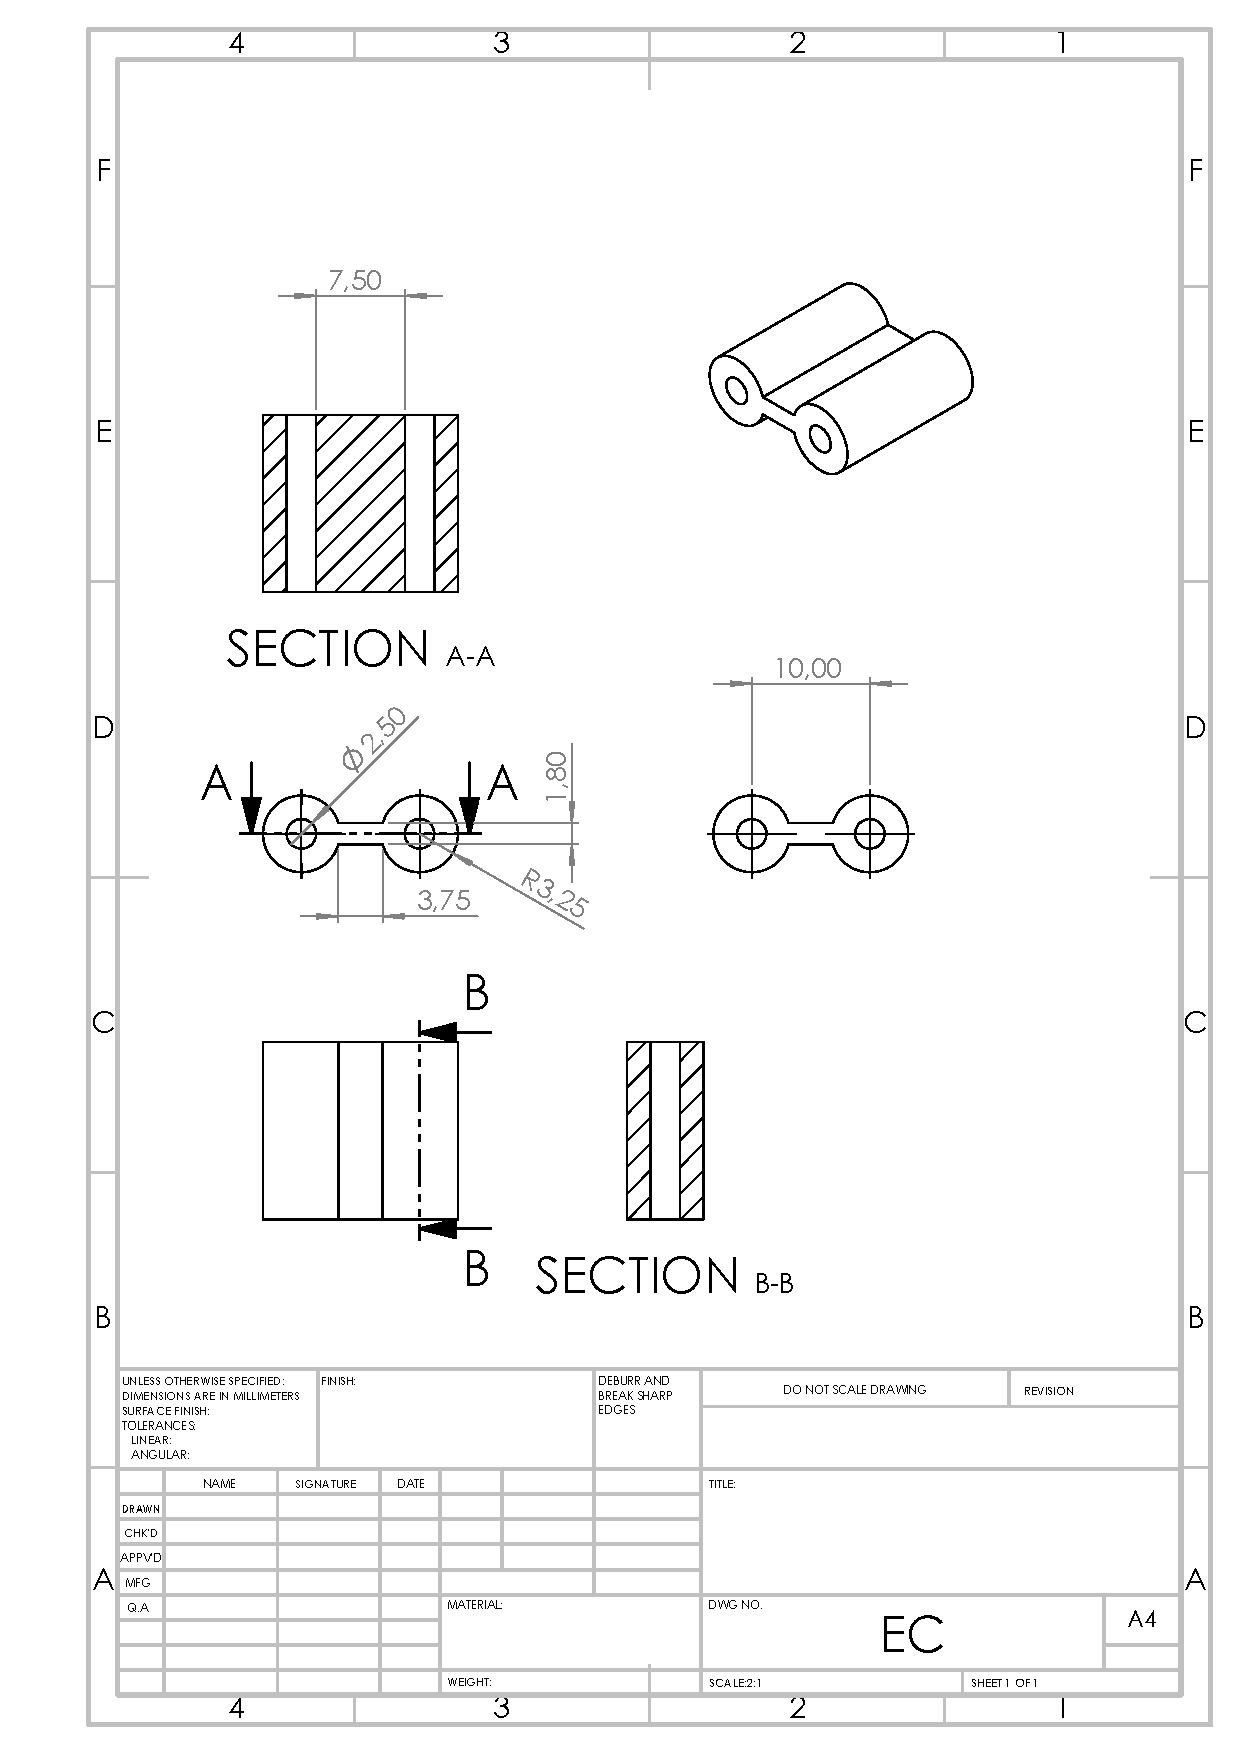
\includegraphics[width=0.62\textwidth]{Embout_EC.pdf}
\schemacap{embout}{Plan de l'embout « EC » (échelle 2:1, cotes en mm) : deux perçages de \qty{2,50}{mm} à \qty{10,00}{mm} d'entraxe, reliés par une fente de \qty{1,80}{mm}.}
\end{figure}

\subsubsection*{Le montage}

Je monte la sonde dans l'ordre qui évite de refaire un travail. On commence par imprimer le tube et l'embout, puis par vérifier qu'une mine glisse dans chaque canal sans forcer : si l'impression a resserré un canal, on le dégage avec le foret. Ensuite on coupe les deux mines à la longueur du tube, soit \qty{66,9}{mm}, plus \qty{15}{mm} côté eau et quelques millimètres côté tête pour le contact, soit environ \qty{87}{mm}, avec la scie fine. On les enfile dans les canaux, de sorte qu'il en dépasse \qty{15}{mm} du côté de la collerette.

On glisse alors l'embout sur les mines, côté tête, pour les maintenir à \qty{10}{mm}. On enroule un fil de cuivre fin, bien serré, autour du haut de chaque mine, avec une goutte de colle conductrice si on en a. Le graphite ne se soude pas : c'est la pression du fil qui fait le contact. Puis on soude chaque fil au câble blindé et on vérifie au multimètre que les deux mines ne se touchent pas.

Enfin on remplit de résine époxy la tête et l'embout, de manière à noyer les fils et les contacts, et on colle les mines dans leurs canaux côté eau pour que l'eau ne remonte pas. On laisse durcir le temps indiqué sur le tube. Seul le graphite doit toucher l'eau.

\begin{attention}
Aucun cuivre ne doit toucher l'eau : il se dissoudrait dans la solution, toxique pour les plantes, et fausserait la mesure. Si un morceau de fil dépasse de la résine, je recommence cette étape.
\end{attention}

% ---------------------------------------------------------------------
\Needspace{8\baselineskip}\subsection{Circuit et mesure}

Cette sous-partie présente d'abord le schéma électrique de la mesure et sa nomenclature. Elle démontre ensuite comment on retrouve la résistance de l'eau à partir de deux lectures, puis décrit le programme de l'Arduino qui fait ces lectures. Elle se termine par l'alternance avec la sonde pH.

\subsubsection*{Le schéma électrique}

Je cherche un montage avec le moins de composants possible. Je relie la broche D5 de l'Arduino à la première mine de la sonde par une résistance de référence $R_1$, et la broche D6 directement à la seconde mine. La broche d'entrée analogique A0 lit la tension au point J, entre $R_1$ et la sonde. Pour inverser le courant, il suffit d'échanger les états de D5 et de D6 : l'une est à \qty{5}{V} pendant que l'autre est à \qty{0}{V}, puis l'inverse.

Je dessine le schéma dans le même style que celui de l'Arduino, en pleine page dans le schéma complet de la tour (page suivante). Je le lis de gauche à droite : l'Arduino (-K2) avec ses broches, puis les composants de la mesure au milieu, puis la sonde de température DS18B20\ix{24} (-B4) à droite. Cette sonde reste sur la broche D2, avec sa résistance de tirage $R_2$ de \qty{4,7}{k\ohm}. Les deux phases du courant sont rappelées sur le schéma. Le courant $I$ représenté est celui de la phase 1.

\schemapaysageC{eagle/schema_complet.pdf}{elcompl}{Schéma électrique complet de la tour (alimentation, commande, capteurs et sonde EC), sur une seule feuille.}

\subsubsection*{La nomenclature}

Chaque repère du schéma renvoie à une ligne du tableau.

\begin{table}[H]
\centering
\small
\begin{tabularx}{\textwidth}{|l|l|l|Y|}
\hline
\textbf{Repère} & \textbf{Désignation} & \textbf{Caractéristiques} & \textbf{Fonction} \\
\hline
-B2 & Sonde de conductivité & Deux mines de graphite 4B & Plonge dans l'eau du bac ; sa résistance $R_w$ dépend de la conductivité. \\
\hline
-B4 & Sonde de température DS18B20\ix{24} & Bus 1-Wire & Donne la température de l'eau pour la compensation. \\
\hline
-K2 & Carte Arduino Uno & Broches D2, D5, D6, A0, \qty{5}{V}, GND & Impose \qty{5}{V} ou \qty{0}{V} sur D5 et D6, lit la tension du point J sur A0 et dialogue avec la sonde de température. \\
\hline
-R1 & Résistance de référence & \qty{340}{\ohm}, 1 \% & Forme avec la sonde un pont diviseur de tension. \\
\hline
-R2 & Résistance de tirage & \qty{4,7}{k\ohm} & Maintient le bus 1-Wire à l'état haut. \\
\hline
-X1 & Bornier du DS18B20\ix{24} & 3 bornes & Raccorde la sonde de température. \\
\hline
\end{tabularx}
\caption{Nomenclature du circuit de mesure de l'EC.}
\end{table}

\subsubsection*{De deux tensions à la résistance de l'eau}

Il me reste à savoir quoi calculer avec les lectures de l'entrée A0. Je mesure la tension au point J dans chacune des deux phases, puis j'en fais le rapport. Je pars de l'hypothèse que chaque broche se comporte comme une source de tension $V$ en série avec une petite résistance : $r_H$ à l'état haut, $r_L$ à l'état bas (en ohms, quelques dizaines d'ohms pour un Arduino).

\naturecalc{théorie (formule démontrée, valeurs de fiches techniques et hypothèses ; rien de mesuré)}
\begin{demonstration}[résistance de l'eau à partir de deux tensions]
\resultat{R_w = R_1 + P\,(x - 1)\quad\text{avec}\quad x = \frac{U_1}{U_2}\ \text{et}\ P = R_1 + r_L}
\textbf{Phase 1 :} D5 à l'état haut, D6 à l'état bas. Le courant traverse, en série, $r_H$, $R_1$, la sonde $R_w$ et $r_L$. Il vaut (en ampères) :
\[
I_1 = \frac{V}{r_H + R_1 + R_w + r_L}
\]
Le point J est situé entre $R_1$ et la sonde. Sa tension $U_1$ (en volts) est la chute de tension dans $R_w$ et $r_L$ :
\begin{align*}
U_1 &= (R_w + r_L)\,I_1\\
U_1 &= V\,\frac{R_w + r_L}{r_H + R_1 + R_w + r_L}
\end{align*}
\textbf{Phase 2 :} D5 à l'état bas, D6 à l'état haut. Le courant traverse $r_H$, la sonde, $R_1$ et $r_L$ : c'est la même somme, donc le même courant, mais en sens inverse :
\[
I_2 = \frac{V}{r_H + R_w + R_1 + r_L} = I_1
\]
Le point J est maintenant situé entre la sonde et $R_1$. Sa tension $U_2$ (en volts) est la chute de tension dans $R_1$ et $r_L$ :
\begin{align*}
U_2 &= (R_1 + r_L)\,I_2\\
U_2 &= V\,\frac{R_1 + r_L}{r_H + R_1 + R_w + r_L}
\end{align*}
Je fais le rapport $x = U_1/U_2$ : $V$, $r_H$ et le dénominateur disparaissent.
\begin{align*}
x &= \frac{U_1}{U_2}\\
x &= \frac{R_w + r_L}{R_1 + r_L}
\end{align*}
J'isole $R_w$ :
\begin{align*}
R_w + r_L &= (R_1 + r_L)\,x\\
R_w &= (R_1 + r_L)\,x - r_L
\end{align*}
Je pose $P = R_1 + r_L$ (en ohms), donc $r_L = P - R_1$ :
\begin{align*}
R_w &= P\,x - (P - R_1)\\
R_w &= R_1 + P\,(x - 1)
\end{align*}
Ce résultat est précieux. Le rapport $x$ ne dépend ni de la tension d'alimentation, ni de la référence du convertisseur, ni de $r_H$. La seule inconnue est $P$, que je mesure à l'étalonnage (partie 7.7). Comme les deux phases font passer le même courant en sens contraire, le courant moyen dans la sonde est nul :
\[
\frac{I_1 + (-I_2)}{2} = 0
\]
ce qui réalise la condition posée à la partie 7.4.
\end{demonstration}

\subsubsection*{Le programme de mesure}

Le Raspberry ne peut pas faire cette mesure lui-même : un aller-retour par le câble USB dure plusieurs millisecondes, alors qu'une phase doit durer environ \qty{130}{\micro s}. Je choisis donc de faire toute la mesure dans l'Arduino, en une seule commande, que j'ajoute au programme \texttt{HydroTour\_Firmata}. Le Raspberry demande la mesure et reçoit en retour les deux sommes $S_1$ et $S_2$. Cette commande a été écrite et installée le 20 novembre 2026 : la partie 9.1 en donne le détail.

L'Arduino répète 64 fois les deux phases. À chaque phase, il attend \qty{20}{\micro s} que la tension se stabilise, puis lit l'entrée A0 et l'ajoute à une somme. Ensuite, il remet les deux broches en entrée pour déconnecter la sonde. Une lecture est un nombre entier de 0 à 1\,023.

L'organigramme suivant résume la commande « mesure EC » dans l'Arduino.

\begin{figure}[H]
\centering
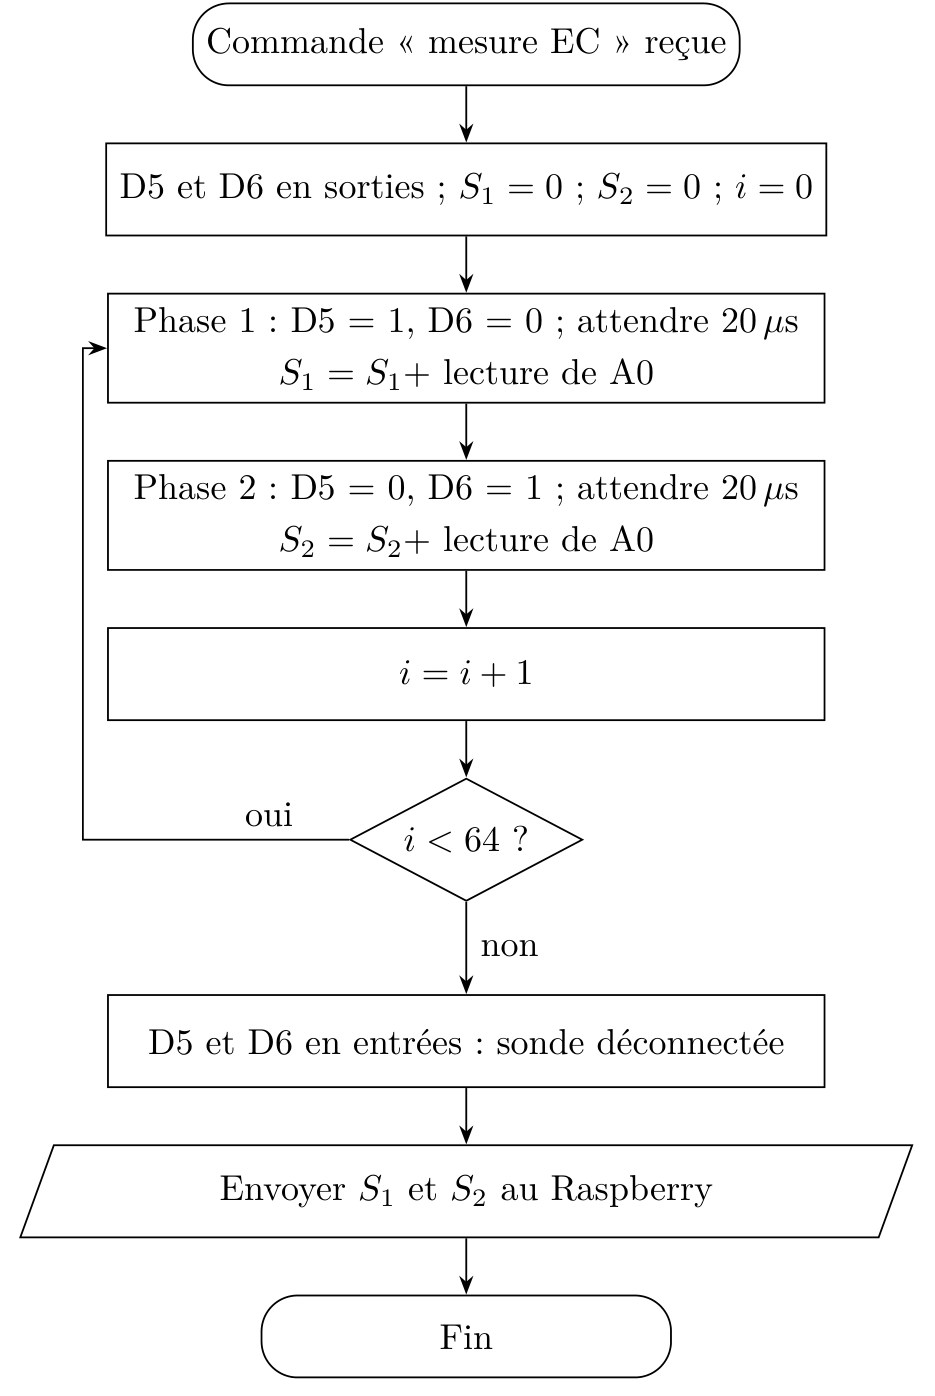
\includegraphics[width=0.5\textwidth]{img/inf/g_orga_ec.png}
\schemacap{orgaec}{Organigramme (ISO 5807) de la commande « mesure EC » dans l'Arduino.}
\end{figure}

\naturecalc{théorie (formule démontrée, valeurs de fiches techniques et hypothèses ; rien de mesuré)}
\begin{demonstration}[durée d'une mesure et taille des sommes]
\resultat{T \approx \qty{17}{ms}\quad\text{et}\quad S_{\max} = 65\,472}
Une phase comprend l'attente de \qty{20}{\micro s} et une lecture analogique, qui dure environ \qty{112}{\micro s} avec le réglage habituel de l'Arduino :
\begin{align*}
t_{\text{phase}} &= \qty{20}{\micro s} + \qty{112}{\micro s}\\
t_{\text{phase}} &= \qty{132}{\micro s} \approx \qty{130}{\micro s}
\end{align*}
Une mesure comprend $64\times 2 = 128$ phases :
\begin{align*}
T &= 128\times\qty{132}{\micro s}\\
T &= \qty{16896}{\micro s}\\
T &\approx \qty{17}{ms}
\end{align*}
Le courant change de sens toutes les \qty{132}{\micro s}, soit une période de \qty{264}{\micro s} (une phase 1 puis une phase 2) et une fréquence de :
\begin{align*}
f &= \frac{1}{\qty{264}{\micro s}}\\
f &\approx \qty{3800}{Hz}
\end{align*}
Chaque somme est au plus égale à 64 lectures de 1\,023 :
\begin{align*}
S_{\max} &= 64\times 1023\\
S_{\max} &= 65\,472
\end{align*}
Cette valeur est inférieure à $65\,535 = 2^{16} - 1$ : un entier de 16 bits suffit pour chaque somme.
\end{demonstration}

Le rapport $x$ se calcule ensuite sur le Raspberry. Les 64 lectures de chaque phase ont la même échelle, donc leur rapport est celui des tensions :
\[
x = \frac{S_1}{S_2} = \frac{U_1}{U_2}
\]

La figure suivante montre l'inversion de la polarité pendant une mesure.

\begin{figure}[H]
\centering
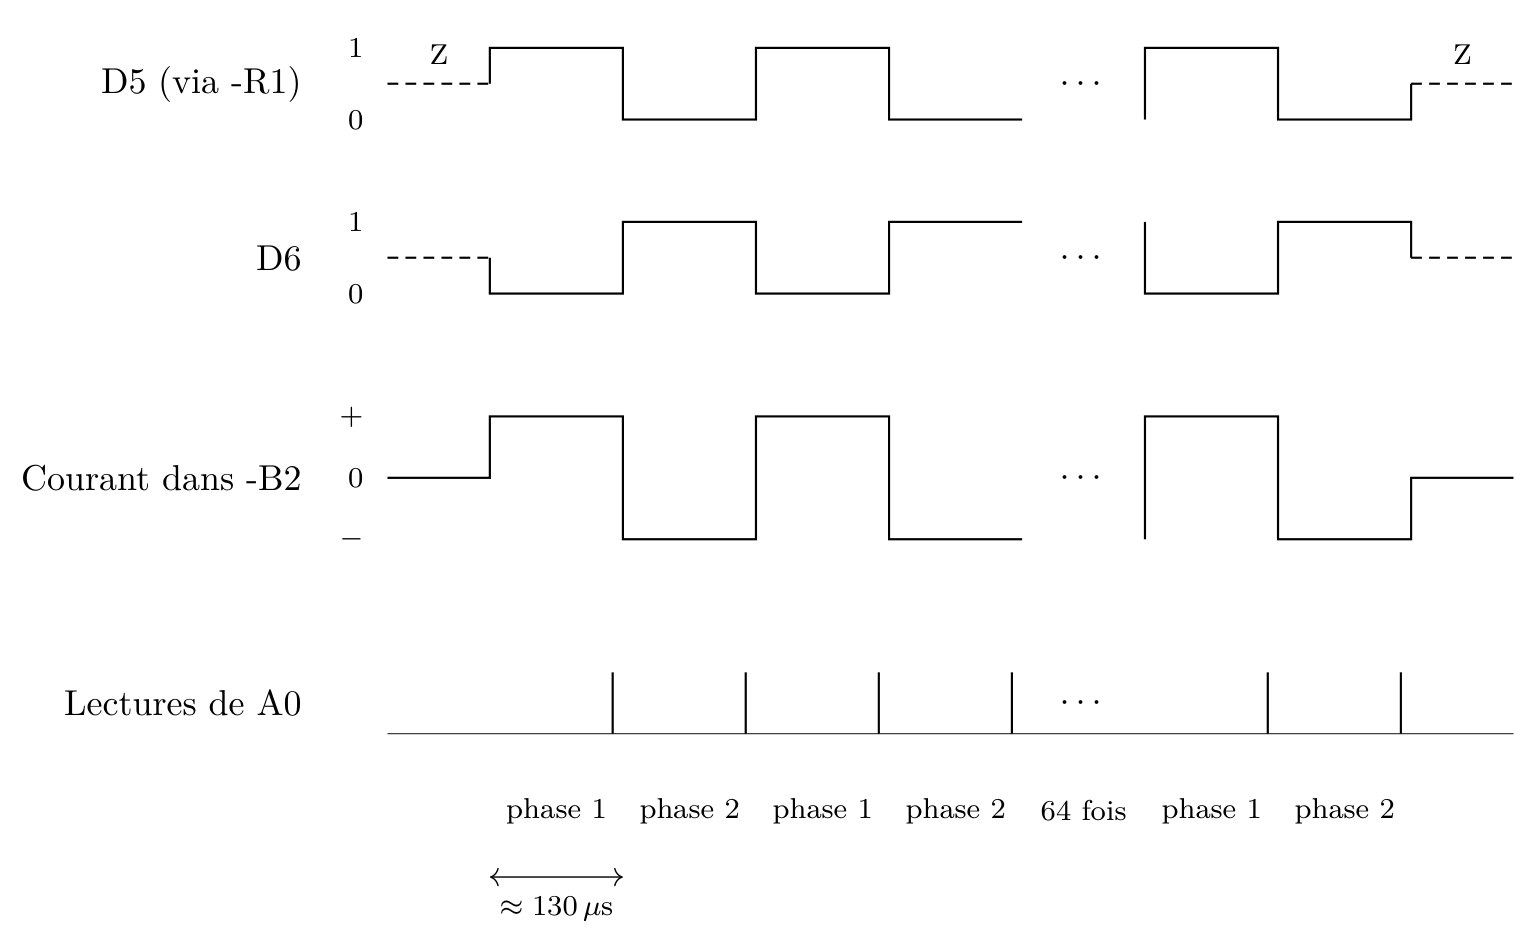
\includegraphics[width=0.92\textwidth]{img/inf/g_inversion.png}
\schemacap{inversion}{Inversion de polarité pendant une mesure. Z : broche en entrée (haute impédance), la sonde n'est reliée à rien.}
\end{figure}

\subsubsection*{L'alternance avec la sonde pH}

Je dois encore m'assurer que la mesure de l'EC ne perturbe pas la sonde pH plongée dans le même bac. Je garde la règle déjà adoptée pour le projet : la carte pH est coupée par la sortie 4 de la carte MOSFET\ix{15} pendant la mesure de l'EC, et le pH n'est pas lu dans les \qty{5}{s} qui suivent. La mesure de l'EC a lieu une fois par minute, alors que le pH est lu toutes les \qty{10}{s} (figure suivante). La lecture du pH prévue à \qty{60}{s} est donc sautée ; la suivante, à \qty{70}{s}, a lieu \qty{9,5}{s} après la mesure.

\begin{figure}[H]
\centering
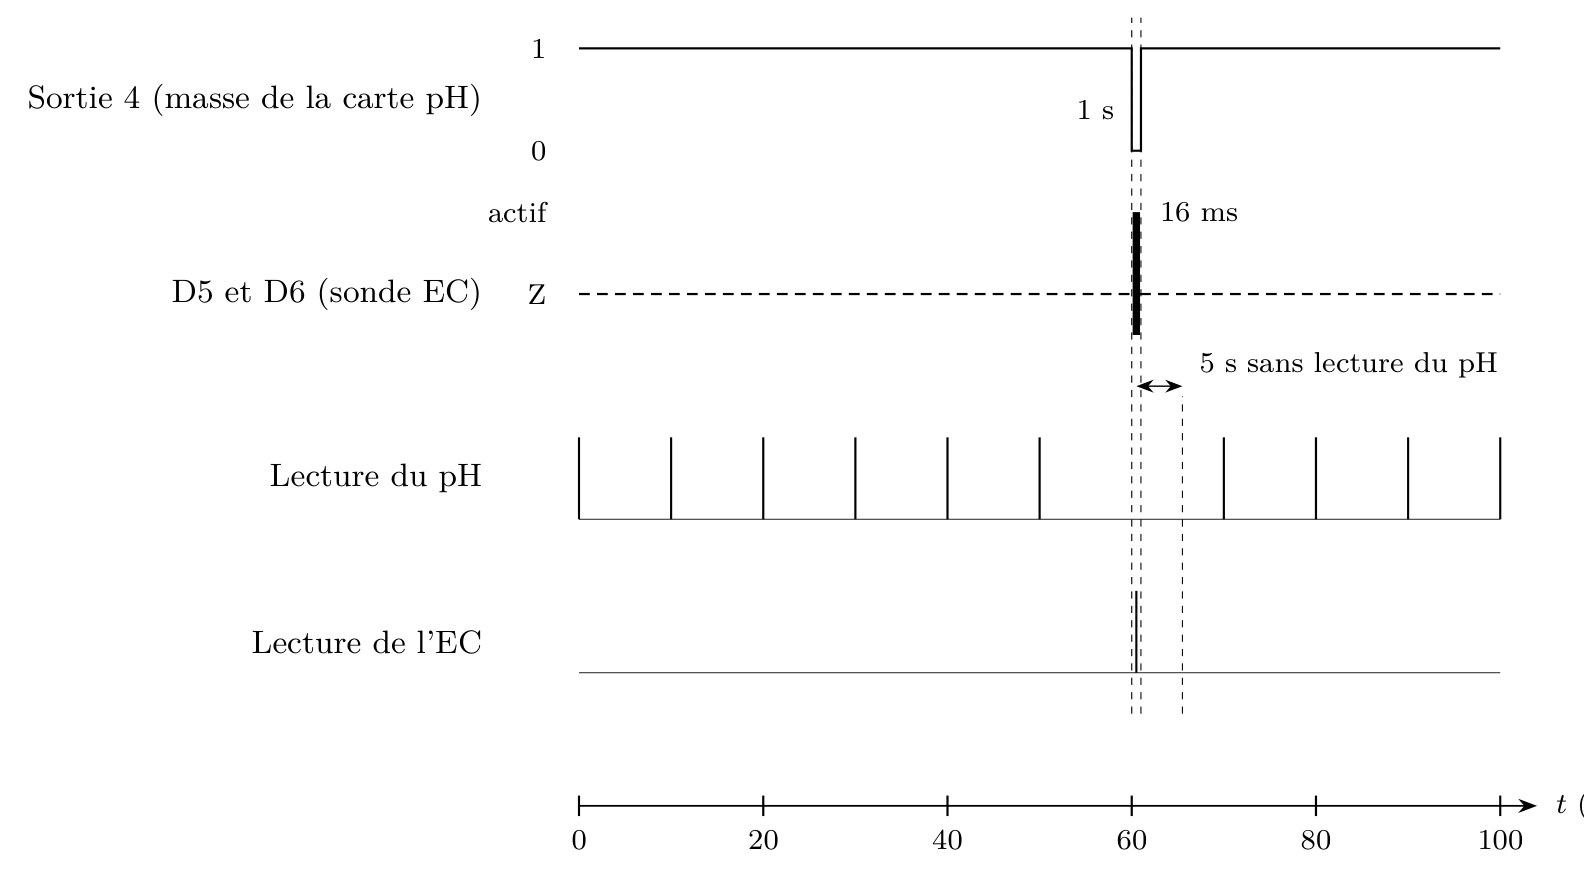
\includegraphics[width=0.92\textwidth]{img/inf/g_deroulement.png}
\schemacap{deroul}{Déroulement sur 100 s : le pH est lu toutes les 10 s, l'EC une fois par minute pendant 16 ms. La sortie 4 coupe la carte pH autour de la mesure.}
\end{figure}

Comme la mesure de l'EC ne dure que \qty{16}{ms} avec un courant moyen nul, ces précautions sont peut-être excessives. Je ne le sais pas : je les garde tant qu'un essai (partie 7.8) ne montre pas qu'on peut les alléger.

\begin{aretenir}
Une mesure de l'EC, c'est 64 allers-retours du courant en environ \qty{17}{ms}, deux sommes $S_1$ et $S_2$ envoyées au Raspberry, et la sonde déconnectée le reste du temps.
\end{aretenir}

% ---------------------------------------------------------------------
\Needspace{8\baselineskip}\subsection{Étalonnage et calcul de l'EC}

Cette sous-partie explique d'abord comment ramener la conductivité à une température de référence. Elle démontre ensuite comment deux solutions étalons donnent la constante de cellule $K$ et la résistance $P$, puis applique le calcul à un exemple chiffré. Elle décrit enfin la procédure d'étalonnage.

\subsubsection*{La température}

La conductivité d'une solution augmente quand elle se réchauffe, car les ions se déplacent plus vite. Le DS18B20\ix{24} donne la température de l'eau ; je ramène chaque mesure à \qty{25}{\celsius}, température de référence des solutions étalons. Pour cela, je suppose que l'augmentation est proportionnelle à l'écart avec \qty{25}{\celsius}, avec un coefficient $\alpha$ d'environ \qty{0,02}{\celsius^{-1}}, soit \qty{2}{\percent} par degré.

\naturecalc{théorie (formule démontrée, valeurs de fiches techniques et hypothèses ; rien de mesuré)}
\begin{demonstration}[conductivité ramenée à \qty{25}{\celsius}]
\resultat{\sigma_{25} = \frac{\sigma_T}{1 + \alpha\,(T - 25)}}
La conductivité $\sigma_T$ mesurée à la température $T$ (en \unit{\celsius}) s'écrit, d'après l'hypothèse, à partir de la conductivité $\sigma_{25}$ à \qty{25}{\celsius} (toutes deux en mS/cm) :
\[
\sigma_T = \sigma_{25} + \alpha\,(T - 25)\,\sigma_{25}
\]
Je mets $\sigma_{25}$ en facteur :
\[
\sigma_T = \sigma_{25}\,\bigl(1 + \alpha\,(T - 25)\bigr)
\]
Je divise par le facteur entre parenthèses :
\[
\sigma_{25} = \frac{\sigma_T}{1 + \alpha\,(T - 25)}
\]
Exemple avec $\sigma_T = \qty{1,20}{mS/cm}$ à $T = \qty{20}{\celsius}$ et $\alpha = \qty{0,02}{\celsius^{-1}}$ :
\begin{align*}
\sigma_{25} &= \frac{\qty{1,20}{mS/cm}}{1 + \qty{0,02}{\celsius^{-1}}\times(\qty{20}{\celsius} - \qty{25}{\celsius})}\\
\sigma_{25} &= \frac{\qty{1,20}{mS/cm}}{1 - 0{,}10}\\
\sigma_{25} &= \frac{\qty{1,20}{mS/cm}}{0{,}90}\\
\sigma_{25} &\approx \qty{1,33}{mS/cm}
\end{align*}
Le dernier signe est $\approx$ car $1{,}20/0{,}90$ ne tombe pas juste : j'arrondis au centième.
\end{demonstration}

\subsubsection*{L'étalonnage avec deux solutions}

Il me reste deux inconnues : la constante de cellule $K$, qui dépend de la forme de la sonde, et la résistance $P = R_1 + r_L$, qui dépend de l'Arduino. Pour les trouver, je plonge la sonde dans deux solutions de conductivité connue : l'une à \qty{1,413}{mS/cm}, proche de la plage de travail, et l'autre à \qty{12,88}{mS/cm}, où la résistance de l'eau est faible et où $r_L$ pèse beaucoup. Chaque solution donne un rapport $x$ et une équation.

\naturecalc{théorie (formule démontrée, valeurs de fiches techniques et hypothèses ; rien de mesuré)}
\begin{demonstration}[constante de cellule $K$ et résistance $P$]
\resultat{P = \frac{R_1\,(\sigma_2 - \sigma_1)}{\sigma_1\,(x_1 - 1) - \sigma_2\,(x_2 - 1)}\quad\text{et}\quad K = \sigma_1\,\bigl(R_1 + P\,(x_1 - 1)\bigr)}
On note $\sigma_1 = \qty{1,413}{mS/cm}$ et $\sigma_2 = \qty{12,88}{mS/cm}$ les conductivités des solutions, et $x_1$ et $x_2$ les rapports $U_1/U_2$ mesurés dedans. D'après la partie 7.6, $R_w = R_1 + P\,(x - 1)$, et d'après la partie 7.5, $R_w = K/\sigma$. Pour chaque solution :
\begin{align*}
\frac{K}{\sigma_1} &= R_1 + P\,(x_1 - 1)\\
\frac{K}{\sigma_2} &= R_1 + P\,(x_2 - 1)
\end{align*}
J'isole $K$ dans la première équation :
\[
K = \sigma_1\,\bigl(R_1 + P\,(x_1 - 1)\bigr)
\]
Je le remplace dans la seconde :
\[
\frac{\sigma_1}{\sigma_2}\,\bigl(R_1 + P\,(x_1 - 1)\bigr) = R_1 + P\,(x_2 - 1)
\]
Je multiplie par $\sigma_2$ :
\[
\sigma_1\,R_1 + \sigma_1\,P\,(x_1 - 1) = \sigma_2\,R_1 + \sigma_2\,P\,(x_2 - 1)
\]
Je regroupe les termes en $P$ d'un côté et les autres de l'autre :
\begin{align*}
\sigma_1\,P\,(x_1 - 1) - \sigma_2\,P\,(x_2 - 1) &= \sigma_2\,R_1 - \sigma_1\,R_1\\
P\,\bigl[\sigma_1\,(x_1 - 1) - \sigma_2\,(x_2 - 1)\bigr] &= R_1\,(\sigma_2 - \sigma_1)\\
P &= \frac{R_1\,(\sigma_2 - \sigma_1)}{\sigma_1\,(x_1 - 1) - \sigma_2\,(x_2 - 1)}
\end{align*}
On en déduit $K$ avec l'expression trouvée plus haut.
\end{demonstration}

Une fois $K$ et $P$ connus, la mesure se fait en trois temps : on calcule $x = S_1/S_2$, puis $R_w = R_1 + P\,(x - 1)$, et enfin $\sigma_T = K/R_w$, que l'on ramène à \qty{25}{\celsius}.

\subsubsection*{Un exemple chiffré}

Pour vérifier que les formules se tiennent, je les applique à des valeurs que je choisis moi-même. Ce ne sont pas des mesures : elles servent seulement à contrôler le calcul. Je suppose $K = \qty{1,200}{cm^{-1}}$, $r_L = \qty{25}{\ohm}$ et $R_1 = \qty{330}{\ohm}$, donc $P = \qty{355}{\ohm}$. Ces trois valeurs sont choisies pour l'exemple et ne sont pas celles du montage : la résistance réellement montée vaut \qty{340}{\ohm}. Seul le déroulement du calcul compte ici.

\begin{exemple}[retrouver $K$ et $P$ à partir de $x_1$ et $x_2$]
Dans la solution à \qty{1,413}{mS/cm}, la résistance de l'eau serait :
\begin{align*}
R_{w1} &= \frac{K}{\sigma_1} = \frac{\qty{1,200}{cm^{-1}}}{\qty{1,413e-3}{S/cm}}\\
R_{w1} &\approx \qty{849,3}{\ohm}
\end{align*}
Le rapport correspondant, d'après $x = (R_w + r_L)/(R_1 + r_L)$, vaut :
\begin{align*}
x_1 &= \frac{\qty{849,3}{\ohm} + \qty{25}{\ohm}}{\qty{355}{\ohm}}\\
x_1 &\approx 2{,}463
\end{align*}
Dans la solution à \qty{12,88}{mS/cm} :
\begin{align*}
R_{w2} &= \frac{\qty{1,200}{cm^{-1}}}{\qty{12,88e-3}{S/cm}} \approx \qty{93,2}{\ohm}\\
x_2 &= \frac{\qty{93,2}{\ohm} + \qty{25}{\ohm}}{\qty{355}{\ohm}} \approx 0{,}333
\end{align*}
Je retrouve $P$ avec la formule démontrée :
\begin{align*}
P &= \frac{\qty{330}{\ohm}\times(\qty{12,88}{mS/cm} - \qty{1,413}{mS/cm})}{\qty{1,413}{mS/cm}\times(2{,}463 - 1) - \qty{12,88}{mS/cm}\times(0{,}333 - 1)}\\
P &= \frac{\qty{330}{\ohm}\times\qty{11,467}{mS/cm}}{\qty{2,067}{mS/cm} + \qty{8,591}{mS/cm}}\\
P &= \frac{\qty{3784}{\ohm.mS/cm}}{\qty{10,658}{mS/cm}}\\
P &\approx \qty{355}{\ohm}
\end{align*}
Puis $K$ :
\begin{align*}
K &= \qty{1,413}{mS/cm}\times\bigl(\qty{330}{\ohm} + \qty{355}{\ohm}\times(2{,}463 - 1)\bigr)\\
K &= \qty{1,413}{mS/cm}\times\qty{849,4}{\ohm}\\
K &\approx \qty{1200}{\ohm.mS/cm}
\end{align*}
Comme $\qty{1}{mS}\times\qty{1}{\ohm} = \num{e-3}$ (en siemens fois ohm, sans unité), on obtient $K \approx \qty{1,200}{cm^{-1}}$, la valeur de départ.

Si la sonde donne ensuite $x = 1{,}50$ dans la solution du bac :
\begin{align*}
R_w &= \qty{330}{\ohm} + \qty{355}{\ohm}\times(1{,}50 - 1)\\
R_w &= \qty{330}{\ohm} + \qty{177,5}{\ohm}\\
R_w &= \qty{507,5}{\ohm}\\
\sigma &= \frac{K}{R_w} = \frac{\qty{1,200}{cm^{-1}}}{\qty{507,5}{\ohm}}\\
\sigma &\approx \qty{2,36e-3}{S/cm} = \qty{2,36}{mS/cm}
\end{align*}
\end{exemple}

\subsubsection*{La procédure d'étalonnage}

Je prévois d'étalonner dans cet ordre, pour ne pas contaminer une solution avec l'autre. On rince d'abord la sonde à l'eau déminéralisée et on l'essuie sans frotter, puis on la plonge dans la solution à \qty{1,413}{mS/cm} en attendant que la température se stabilise. Ensuite on laisse le Raspberry enregistrer plusieurs mesures de suite et on en garde la moyenne, qui donne $x_1$. On rince de nouveau la sonde, on recommence avec la solution à \qty{12,88}{mS/cm}, ce qui donne $x_2$. Le Raspberry calcule alors $K$ et $P$ avec la formule de la partie 7.7 et les enregistre, comme il le fait déjà pour le pH.

Pour contrôler le résultat, on replonge la sonde dans la solution à \qty{1,413}{mS/cm} : la valeur affichée doit s'en approcher à quelques pour cent près. Les boutons d'étalonnage de l'EC ne sont pas encore dans le dashboard.

\begin{attention}
Les solutions étalons sont données pour \qty{25}{\celsius}. Si elles sont à une autre température, j'applique la même compensation qu'à la partie 7.7 avant de calculer $K$ et $P$.
\end{attention}

% ---------------------------------------------------------------------
\Needspace{8\baselineskip}\subsection{Essais et limites de la sonde EC}

Cette sous-partie dit d'abord ce qui est vérifié aujourd'hui, puis les essais que je prévois sur la vraie sonde. Elle se termine par un tableau de synthèse de l'état d'avancement.

\subsubsection*{Ce qui est vérifié}

Je préfère être clair : à ce jour, aucune mesure n'a été faite avec cette sonde. L'étude de conception est terminée : la géométrie, le circuit, les calculs et le déroulement de la mesure sont posés et démontrés. La sonde n'est pas construite, la commande n'est pas écrite dans l'Arduino et aucun étalonnage n'a été fait. Les exemples chiffrés de la partie 7.7 sont des valeurs que j'ai choisies, pas des mesures.

\subsubsection*{Les essais prévus}

Je prévois de tester la sonde étape par étape, dans l'ordre où les erreurs coûtent le moins cher. On commence par vérifier au multimètre, avant de verser la résine, que les deux mines ne se touchent pas. Une fois la sonde terminée, on la plonge dans la solution à \qty{1,413}{mS/cm} et on compare la résistance de l'eau calculée à la plage attendue de la partie 7.5. Ensuite on étalonne avec les deux solutions, puis on vérifie la répétabilité : dix mesures de suite dans la même solution doivent donner presque la même valeur.

Il faut ensuite mesurer l'effet sur le pH : on lit le pH dans une solution tampon avec, puis sans mesure de l'EC dans le même bac. Si l'écart est négligeable, on peut alléger la coupure de la carte pH de la partie 7.6. Enfin, on refait l'étalonnage après une semaine dans la solution nutritive, pour savoir si la sonde en graphite dérive ou s'encrasse, et à quelle fréquence il faut la nettoyer.

\begin{attention}
Un ohmmètre de multimètre travaille en courant continu : dans l'eau, il affiche une valeur qui dérive (partie 7.4). Il ne sert qu'à détecter un court-circuit, jamais à mesurer la résistance de l'eau.
\end{attention}

\subsubsection*{Synthèse}

Ce tableau reprend chaque fonction de la sonde avec la solution retenue et son état.

\begin{table}[H]
\centering
\small
\begin{tabularx}{\textwidth}{|l|Y|l|}
\hline
\textbf{Fonction} & \textbf{Solution retenue} & \textbf{État} \\
\hline
Électrodes & deux mines de graphite 4B de \qty{1,8}{mm}, entraxe \qty{10}{mm}, tube et embout imprimés en 3D & plans dessinés \\
\hline
Courant alternatif & inversion de polarité à environ \qty{3800}{Hz} & programmé \\
\hline
Circuit & $R_1 = \qty{340}{\ohm}$, broches D5 et D6, lecture sur A0 & monté \\
\hline
Conversion en $R_w$ & rapport $x = S_1/S_2$ puis $R_w = R_1 + P\,(x-1)$ & démontré \\
\hline
Commande de mesure & 64 allers-retours, sommes $S_1$ et $S_2$ & écrite et installée (partie 9.1) \\
\hline
Température & compensation à \qty{25}{\celsius}, $\alpha = \qty{0,02}{\celsius^{-1}}$ & démontré \\
\hline
Étalonnage & deux solutions, conductivités au choix & écrit, essai à faire \\
\hline
Sonde pH & carte coupée pendant la mesure, pas de lecture dans les \qty{5}{s} & à essayer \\
\hline
\end{tabularx}
\caption{Synthèse de la sonde EC fabriquée.}
\end{table}

\begin{aretenir}
La conception est complète. La commande de mesure est écrite et donne sa première valeur dans l'eau depuis le 20 novembre 2026 (partie 9.4), mais la sonde n'est pas encore étalonnée : il reste à faire l'étalonnage à deux solutions avant de pouvoir parler de précision.
\end{aretenir}


% =====================================================================
% PARTIE 7 : LA COMMANDE ET L'INFORMATIQUE (etude informatique v2.4, texte integral)
\clearpage
\partieENO{La commande et l'informatique}

Cette partie reprend en entier l'étude informatique de la tour : la commande automatique, l'accès à distance, la mise en service et les premières mesures réelles. Au départ, le Raspberry lit déjà la sonde pH et la batterie par l'intermédiaire de l'Arduino, mais la pompe ne se commande qu'à la main depuis le dashboard : la tour mesure, mais n'agit pas seule. Pour la rendre autonome, il faut qu'un programme prenne lui-même les décisions : quand arroser, quand ajouter de l'engrais, quand économiser la batterie.

Je commence par présenter le système (8.1), puis le matériel et le câblage (8.2). Je décris ensuite le programme de l'Arduino (8.3) et celui du Raspberry Pi (8.4), puis le dashboard (8.5). Je traite l'accès à distance et la sécurité (8.6), la mise en service sur le matériel (8.7) et les premières mesures réelles (8.8). Je termine par les essais (8.9), la synthèse (8.10), l'organisation des fichiers (8.11) et un rappel de la première version du programme (8.12). La fabrication de la sonde EC fait l'objet de la partie 7, et le dashboard de démonstration celui de la partie 9.

\begin{attention}
Le schéma officiel de la carte Arduino Uno, qui donne les noms des broches, est reproduit ci-dessous (il est aussi dans l'Annexe 5, à la fin du rapport). Pour bien lire les parties 7 à 9, trois points. Premièrement, ces parties décrivent le système final, mais le montage réel avance par étapes : les captures, les valeurs d'exemple et les relevés des parties 8.5 à 9 viennent d'un Arduino simulé ou des premières mesures réelles de la partie 8.8, et le tableau de synthèse (8.10) dit, fonction par fonction, ce qui est vérifié sur le matériel. Deuxièmement, la sonde EC du système final est la sonde fabriquée de la partie 7, lue directement par l'Arduino (broches D5, D6 et A0) avec sa propre constante $K$ ; la sonde du commerce (DFRobot DFR0300, $K = 1$, lue par l'ADS1115\ix{16}) était celle du système de départ, et seul l'exemple de la partie 8.4 en garde la trace. Troisièmement, au début le pH est lu directement par l'entrée A1 de l'Arduino ; dans le montage final, il l'est par l'ADS1115\ix{16} (entrée A0), plus précis.
\end{attention}

\schemapaysageC[page=1]{A000066-schematics.pdf}{uno1}{Schéma électrique officiel de la carte Arduino Uno Rev3 (référence A000066), publié par le constructeur : alimentation, microcontrôleur et liaison USB. Les noms des broches (D5, D6, A0, A4, A5...) servent de repère pour lire les feuilles de commande de la partie 8.2.}
\schemapaysageC[page=2]{A000066-schematics.pdf}{uno2}{Schéma électrique officiel de la carte Arduino Uno Rev3 (suite) : les connecteurs.}

% ---------------------------------------------------------------------
\Needspace{8\baselineskip}\subsection{Présentation du système}

Avant d'entrer dans le détail des choix, cette sous-partie présente chaque élément du système, pour qu'on sache de quoi il est fait et à quoi il sert. Elle commence par ce que le programme doit faire, sous forme de cinq missions, puis explique pourquoi je confie les décisions au Raspberry et l'exécution à l'Arduino. Après une vue d'ensemble du système, elle détaille chaque élément : les cartes électroniques, les capteurs, les pompes et les programmes. Elle présente ensuite le serveur, qui fait tourner la tour, et le dashboard, qui permet de la surveiller de près comme de loin, avant d'expliquer pourquoi certaines mesures doivent être faites en alternance.

\subsubsection*{Ce que fait le programme}

Avant d'écrire une ligne de code, je liste ce que la tour doit faire seule. J'en tire cinq missions, qui servent de cahier des charges pour toute la suite : chaque partie du programme répond à l'une d'elles. Je mets la protection au même niveau que l'arrosage, car une pompe qui tourne à sec ou une batterie vidée à fond peuvent abîmer le matériel pour de bon.

\begin{itemize}
\item \textbf{Mesurer} toutes les 10 secondes : pH, conductivité (EC), températures de l'eau et de l'air, humidité, pression, lumière, niveau du réservoir et état de la batterie.
\item \textbf{Arroser} : la pompe principale tourne par cycles (\qty{15}{min} de marche, \qty{15}{min} d'arrêt par défaut).
\item \textbf{Nourrir} : les pompes doseuses ajoutent l'engrais A, l'engrais B ou le correcteur pH$-$ par petites doses, selon le légume cultivé et son stade.
\item \textbf{Protéger} la batterie, la pompe et les plantes : coupure quand la batterie est basse, arrêt quand le réservoir est presque vide, nombre de doses limité.
\item \textbf{Montrer} tout cela sur un dashboard web, consultable depuis la maison ou depuis Internet après connexion, et sur le petit écran de la tour.
\end{itemize}

\subsubsection*{Le Raspberry décide, l'Arduino exécute}

J'ai deux cartes à disposition : le Raspberry Pi et l'Arduino Uno. J'hésite entre deux solutions : écrire tout le programme dans l'Arduino, ou ne lui laisser que la lecture des capteurs et la commande des pompes. L'Arduino a des entrées analogiques et supporte bien le \qty{5}{V}, mais il a peu de mémoire, pas d'heure fiable, ni base de données ni réseau. Le Raspberry, lui, fait tourner Python, garde l'historique et sert le dashboard. Je choisis donc de mettre toute l'intelligence dans le Raspberry, et de garder le protocole Firmata déjà utilisé dans le projet, pour ne jamais avoir à reprogrammer l'Arduino quand je change une règle.

L'Arduino est relié aux capteurs et aux pompes : ce sont les « yeux et les mains » de la tour. Le Raspberry Pi est le « cerveau » : il reçoit les mesures, décide de ce qu'il faut faire, enregistre l'historique et fait tourner le dashboard. Les deux cartes se parlent par le câble USB avec le protocole Firmata.

\begin{aretenir}
L'Arduino ne prend aucune décision, sauf une : si le Raspberry se tait pendant 30 secondes, il coupe toutes les pompes par sécurité (partie 8.3). Il ne surveille pas encore le niveau d'eau lui-même : c'est le Raspberry qui le fait.
\end{aretenir}

\subsubsection*{Vue d'ensemble}

Avant de câbler, je dessine l'ensemble du système pour vérifier que chaque élément a sa place et qu'aucune liaison n'est oubliée. Je le présente sous la forme d'un schéma synoptique normalisé (IEC 61082-1) : chaque élément est un bloc portant un repère selon IEC 81346, dont la lettre indique la fonction (G : production d'énergie, T : conversion, C : stockage, F : protection, K : traitement de l'information, B : capteur, Q : commutation de puissance, M : entraînement, P : affichage). Les traits forts portent l'énergie, les traits fins les signaux, et les symboles du panneau, du convertisseur, de la batterie, du fusible et des moteurs sont ceux de la norme IEC 60617. Les sous-parties suivantes présentent ces éléments un par un, en reprenant leurs repères.

\begin{figure}[H]
\centering
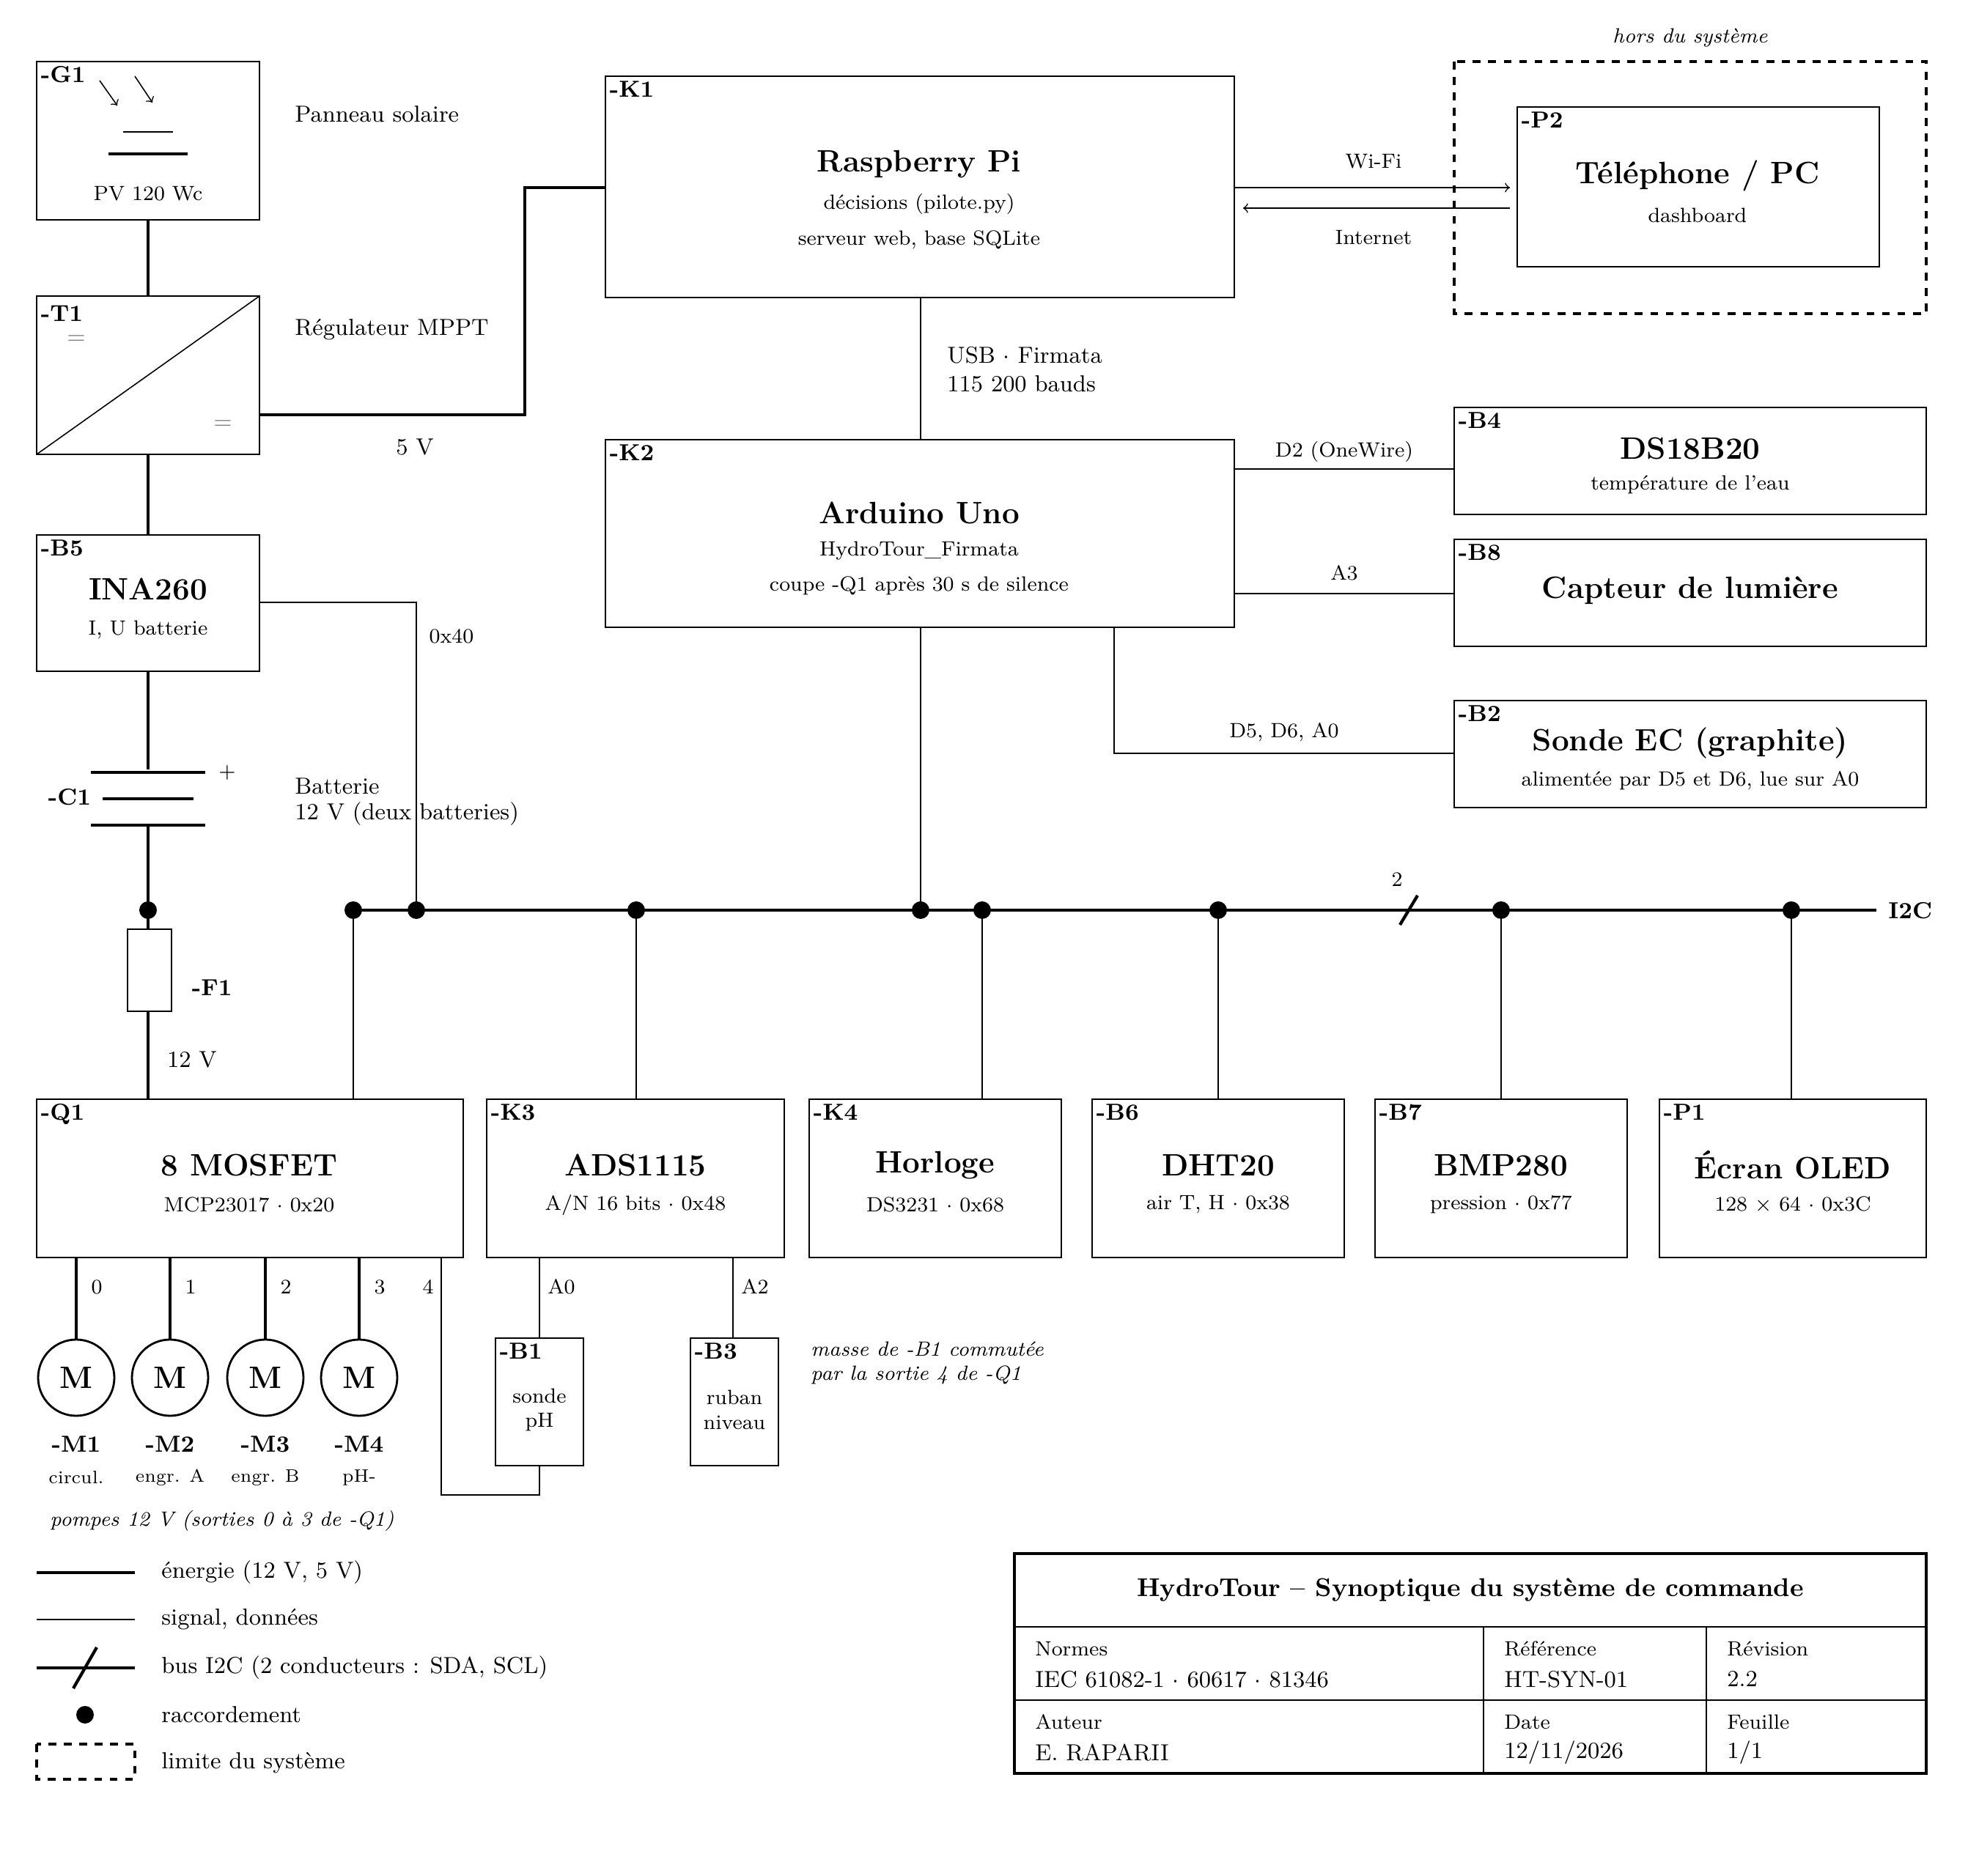
\includegraphics[width=\textwidth]{img/inf/f_synoptique.png}
\schemacap{synop}{Synoptique du système de commande, selon IEC 61082-1 (repères IEC 81346, symboles IEC 60617). Il représente le montage visé ; en attendant l'ADS1115, la sonde pH est branchée sur l'entrée A1 de -K2 (partie 8.2).}
\end{figure}

Ce synoptique montre les blocs. Pour câbler, il me faut le schéma électrique, que je dessine dans le style du schéma officiel de l'Arduino Uno : cadre à cases, fils verts, repères sur chaque composant et cartouche. Il tient sur une seule feuille vectorielle, présentée sur la page suivante en pleine page : alimentation et puissance (panneau, régulateur MPPT\ix{19}, INA260\ix{22}, batteries, fusibles, UBEC\ix{17}), commande (Raspberry Pi, Arduino, bus I2C\ix{12}, carte MOSFET\ix{15}, pompes) et capteurs, dont la sonde EC.

\schemapaysageC{eagle/schema_complet.pdf}{elcompl}{Schéma électrique complet de la tour (alimentation, commande, capteurs et sonde EC), sur une seule feuille.}

\subsubsection*{Les cartes électroniques}

Je cherche à comprendre ce que chaque carte sait faire avant de lui confier un rôle. Quatre cartes forment la chaîne qui va du programme jusqu'aux pompes : chacune compense une limite de la précédente. Le Raspberry ne sait pas lire une tension, l'Arduino la lit mais pas assez finement, et aucun des deux ne peut fournir le courant d'une pompe \qty{12}{V}.

\textbf{-K1 : Raspberry Pi.} Ce que c'est : un ordinateur complet de la taille d'une carte bancaire, sous Linux, avec Wi-Fi et carte mémoire. Son rôle : faire tourner le serveur en Python, prendre les décisions, garder l'historique des mesures et servir le dashboard. Il est alimenté en \qty{5}{V} et relié à l'Arduino par USB.

\textbf{-K2 : Arduino Uno.} Ce que c'est : une carte à microcontrôleur (ATmega328P, \qty{16}{MHz}, \qty{2}{Ko} de mémoire vive) qui lit et commande des broches électriques. Son rôle : faire l'interface entre le Raspberry et le matériel : bus I2C\ix{12}, sonde de température, capteur de lumière, sécurité des pompes. Elle dispose de 6 entrées analogiques, 14 broches numériques et d'un bus I2C\ix{12}.

\textbf{-Q1 : carte 8 MOSFET\ix{15} (Adafruit 6318).} Ce que c'est : huit interrupteurs électroniques (transistors MOSFET\ix{15}) commandés par une puce MCP23017 en I2C\ix{12}, avec une diode de protection et une LED par sortie. Son rôle : allumer et éteindre les quatre pompes \qty{12}{V} et l'alimentation des sondes pH et EC. Elle accepte de \qty{3}{V} à \qty{24}{V}, \qty{3,6}{A} par sortie, à l'adresse 0x20.

\textbf{-K3 : convertisseur ADS1115\ix{16}.} Ce que c'est : un convertisseur analogique-numérique à 4 entrées, beaucoup plus précis que celui de l'Arduino. Son rôle : transformer en nombres les tensions de la sonde pH et du ruban de niveau (la sonde EC est lue directement par l'Arduino). Il travaille sur 16 bits avec un pas de \qty{0,19}{mV}, à l'adresse 0x48.

\subsubsection*{Les capteurs}

Pour chaque capteur, je m'intéresse à son principe de mesure : c'est lui qui explique les précautions à prendre, comme l'étalonnage de la sonde pH, la correction en température de l'EC ou l'alternance entre les deux sondes. Les capteurs se répartissent en deux groupes : ceux de l'eau, qui servent à doser, et ceux de l'énergie et de l'air.

\textbf{Les capteurs de l'eau.}

\textbf{-B1 : sonde pH (DFRobot SEN0161-V2).} Une électrode de verre produit une petite tension qui varie d'environ \qty{59}{mV} par unité de pH. La carte qui l'accompagne l'amplifie et la décale : environ \qty{1,5}{V} à pH 7, et la tension monte quand l'eau devient plus acide. La sonde vieillit et doit être étalonnée dans deux solutions tampon (pH 7 et pH 4).

\naturecalc{théorie (formule démontrée, valeurs de fiches techniques et hypothèses ; rien de mesuré)}
\begin{demonstration}[pente de l'électrode de verre]
\resultat{\dfrac{RT\ln 10}{F} \approx \qty{59,16}{mV}\ \text{par unité de pH à \qty{25}{\celsius}}}
La tension de l'électrode varie comme le logarithme de l'activité des ions $\mathrm{H^+}$. Une variation d'une unité de pH multiplie cette activité par $10$, donc ajoute $\ln 10$ au logarithme. La tension varie alors de :
\[
\Delta U = \frac{R\,T}{F}\,\ln 10
\]
avec $R = \qty{8,314}{J/(mol.K)}$ la constante des gaz parfaits, $T = \qty{298,15}{K}$ la température absolue (\qty{25}{\celsius}) et $F = \qty{96485}{C/mol}$ la constante de Faraday. On calcule ligne par ligne :
\begin{align*}
R\,T &= \qty{8,314}{J/(mol.K)} \times \qty{298,15}{K} = \qty{2478,8}{J/mol}\\
R\,T\,\ln 10 &= \qty{2478,8}{J/mol} \times 2{,}3026 = \qty{5707,7}{J/mol}\\
\Delta U &= \frac{\qty{5707,7}{J/mol}}{\qty{96485}{C/mol}}\\
\Delta U &\approx \qty{0,05916}{V} \approx \qty{59,16}{mV}
\end{align*}
Je l'arrondis à \qty{59}{mV} par unité de pH dans le texte.
\end{demonstration}

\textbf{-B2 : sonde EC fabriquée (deux mines de graphite 4B).} Deux électrodes, ici deux mines de crayon en graphite montées dans un tube imprimé, font passer un courant alternatif dans l'eau. Plus l'eau contient de sels dissous, donc d'engrais, mieux elle conduit le courant. L'EC donne ainsi la quantité de nutriments disponibles. Je fabrique cette sonde moi-même parce que la commande de la sonde du commerce (DFRobot DFR0300) tarde à arriver (partie 7). Sa constante de cellule $K$ est estimée entre \qty{0,97}{cm^{-1}} et \qty{3,04}{cm^{-1}} (elle sera fixée à l'étalonnage) et elle couvre de \qtyrange{0,5}{3,0}{mS/cm}. Elle n'a pas de carte d'interface : l'Arduino la branche lui-même, par les broches D5 et D6 (courant alternatif, en série avec une résistance de \qty{330}{\ohm}), et lit la tension sur l'entrée A0. Elle dépend de la température, d'où la correction à \qty{25}{\celsius}, et elle s'étalonne avec deux solutions de KCl (partie 7.7). Elle n'est ni construite ni testée à ce jour.

\textbf{-B3 : ruban de niveau eTape\ix{23} (\qty{30}{cm}).} La pression de l'eau écrase l'enveloppe du ruban, qui court-circuite une partie de sa piste résistive : plus l'eau monte, plus sa résistance baisse (environ \qty{2000}{\ohm} à vide et \qty{400}{\ohm} plein). Monté en série avec une résistance de \qty{560}{\ohm}, il donne une tension lue par l'ADS1115\ix{16}.

\textbf{-B4 : sonde de température DS18B20\ix{24}.} Un capteur numérique étanche : il envoie directement la température sur un seul fil (protocole OneWire), avec un contrôle d'erreur. Sa précision est de \qty{\pm0,5}{\celsius}. La température de l'eau sert à corriger l'EC et à surveiller les racines.

\textbf{Les capteurs de l'énergie et de l'air.}

\textbf{-B5 : capteur de batterie INA260\ix{22}.} Le courant de la batterie traverse une très petite résistance de \qty{2}{m\ohm} placée dans le module ; la tension à ses bornes donne le courant, positif en charge, négatif en décharge. Il mesure aussi la tension de la batterie, au millivolt près. Le serveur en déduit le pourcentage de charge restant.

\textbf{-K4 : horloge DS1307.} Une horloge à pile qui garde l'heure quand tout est éteint. Sans Internet, le Raspberry ne connaît pas l'heure après une coupure : il la reprend sur cette horloge, pour que les mesures et le calendrier des légumes restent justes.

\textbf{-B6, -B7, -B8, -P1 : Sensor Kit Arduino.} Une carte qui regroupe plusieurs modules prêts à brancher : le DHT20\ix{24} (température et humidité de l'air), le BMP280 (pression de l'air), un capteur de lumière analogique et un écran OLED de $128 \times 64$ points qui affiche les mesures sur la tour.

\textbf{Pourquoi la lumière en \% ?} Le capteur de lumière du kit n'est pas étalonné : il donne une valeur relative, pas des lux. Je l'affiche donc en pourcentage de sa pleine échelle. Il sert surtout à savoir s'il y a du soleil pour relancer la pompe (partie 8.4).

\subsubsection*{Les pompes}

La tour utilise deux sortes de pompes, parce que les besoins sont opposés : déplacer beaucoup d'eau pour arroser, et verser quelques millilitres très précis pour doser. Je garde des pompes en \qty{12}{V} pour qu'elles fonctionnent directement sur la batterie solaire, sans onduleur.

\textbf{-M1 : pompe principale (circulation).} Une pompe immergée de \qty{12}{V} et \qty{19}{W}, prévue dans la nomenclature (jusqu'à \qty{800}{L/h} et \qty{5}{m} de hauteur). Elle remonte la solution nutritive en haut de la tour, d'où elle redescend le long des racines. C'est l'appareil qui consomme le plus : c'est elle qu'on coupe en premier quand la batterie baisse. Elle est sur la sortie 0 de la carte 8 MOSFET\ix{15}.

\textbf{-M2 à -M4 : pompes doseuses péristaltiques\ix{8}.} Des galets écrasent un tuyau souple en tournant et poussent devant eux un volume de liquide toujours identique. Le liquide ne touche que le tuyau, ce qui convient aux engrais et à l'acide. Leur débit d'au plus \qty{100}{mL/min} permet des doses de quelques millilitres : engrais A, engrais B et correcteur pH$-$. Elles sont sur les sorties 1, 2 et 3, en \qty{12}{V}, \qtyrange{0,2}{0,3}{A}.

\subsubsection*{Les programmes}

Je découpe le logiciel en plusieurs programmes, chacun avec une seule responsabilité. Ainsi, une modification des règles de dosage ne touche ni la communication avec l'Arduino ni le dashboard, et chaque morceau peut être testé séparément.

Le tableau suivant liste les programmes du système et le rôle de chacun.

\begin{table}[H]
\centering
\small
\begin{tabularx}{\textwidth}{|l|l|l|Y|}
\hline
\textbf{Programme} & \textbf{Où il tourne} & \textbf{Langage} & \textbf{Rôle} \\
\hline
\texttt{HydroTour\_Firmata} & Arduino & C++ & lire les capteurs et commander les sorties sur ordre ; sécurité de 30 s \\
\hline
\texttt{arduino.py} & Raspberry & Python & dialoguer avec l'Arduino, lire chaque capteur, allumer les pompes \\
\hline
\texttt{pilote.py} & Raspberry & Python & prendre les décisions : cycle, batterie, soleil, dosage, alertes \\
\hline
\texttt{server.py} & Raspberry & Python (Flask) & le serveur : boucle de mesure, base de données, site web \\
\hline
\texttt{hydrotour.html} & navigateur & HTML, JavaScript & le dashboard, avec la tour en 3D \\
\hline
\texttt{hydrotour.db} & Raspberry & SQLite & la base de données : mesures, réglages, stock, légume \\
\hline
\texttt{essai\_materiel.py} & Raspberry & Python & essai de tout le matériel avant la mise en route \\
\hline
\texttt{acces.py} & Raspberry & Python & page de connexion, captcha et réglage de l'identifiant et du mot de passe (partie 8.6) \\
\hline
\texttt{diagnostic.py} & Raspberry & Python & liste ce qui répond vraiment sur l'Arduino (partie 8.7) \\
\hline
\end{tabularx}
\caption{Les programmes du système.}
\end{table}

\subsubsection*{Le serveur}

Le serveur est le programme qui fait vivre la tour. J'ai besoin d'un programme qui tourne en permanence sur le Raspberry et qui fasse deux choses à la fois : piloter la tour sans interruption, et répondre au dashboard dès qu'on l'ouvre. Je choisis Python avec la bibliothèque Flask, simple et légère, qui suffit largement pour un seul utilisateur et fonctionne bien sur un Raspberry.

Un serveur est un programme qui attend des demandes et y répond. Celui de la tour est lancé automatiquement au démarrage du Raspberry par un service du système (partie 8.7). Il écoute sur deux ports : le 5000 pour les appareils du réseau de la maison, et le 5001, réservé à l'accès par Internet (partie 8.6). À l'intérieur, deux tâches tournent en parallèle :

\begin{itemize}
\item la \textbf{boucle de pilotage}, toutes les 10 s : elle lit les capteurs par l'Arduino, demande ses décisions au pilote, commande les pompes, enregistre la mesure dans la base et met à jour l'écran ;
\item le \textbf{serveur web} : il envoie la page du dashboard, puis répond à ses demandes (dernière mesure, historique, réglages, commandes manuelles).
\end{itemize}

Le schéma suivant montre comment la boucle de pilotage et le serveur web tournent en même temps dans le serveur.

\begin{figure}[H]
\centering
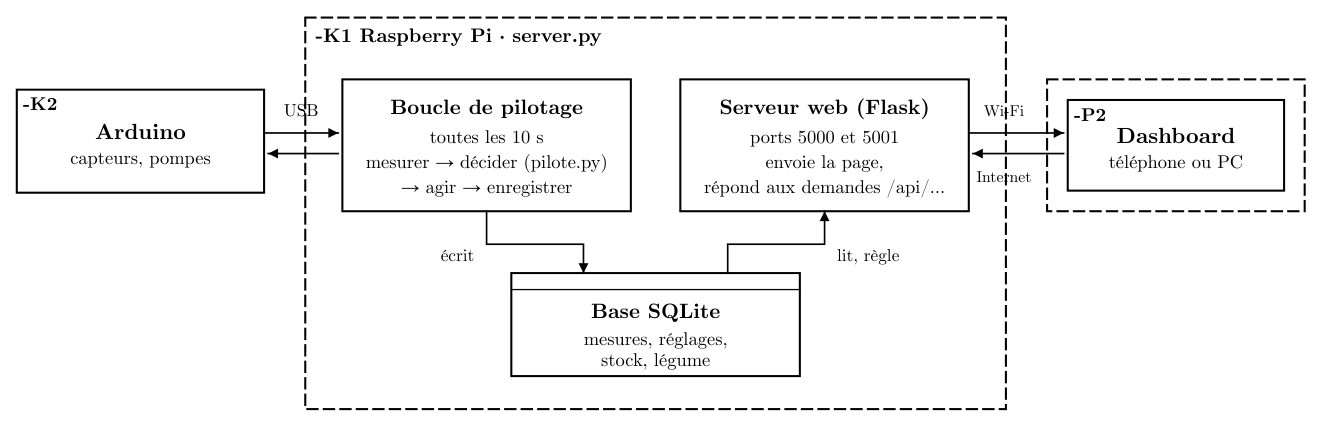
\includegraphics[width=0.95\textwidth]{img/inf/f_serveur.png}
\schemacap{serveur}{Le serveur : la boucle de pilotage et le serveur web tournent en même temps et partagent la même base de données.}
\end{figure}

Le dashboard dialogue avec le serveur par des adresses web simples, appelées API :

\begin{table}[H]
\centering
\small
\begin{tabularx}{\textwidth}{|l|Y|}
\hline
\textbf{Adresse} & \textbf{Ce qu'elle fait} \\
\hline
\texttt{/api/latest} & dernière mesure, état des pompes, alertes et journal du pilote \\
\hline
\texttt{/api/history} & historique des mesures pour les courbes et l'export en tableur \\
\hline
\texttt{/api/pompe} & commande manuelle : démarrer ou arrêter la circulation, dose de quelques secondes \\
\hline
\texttt{/api/pilotage} & lire ou changer les réglages : automatique, cycle, seuils de batterie \\
\hline
\texttt{/api/culture} & légume cultivé et date de plantation, d'où le serveur déduit les cibles \\
\hline
\texttt{/api/etalonner} & enregistrer l'étalonnage du pH (7 et 4) et du réservoir (vide et plein) \\
\hline
\texttt{/api/stock}, \texttt{/api/batterie} & litres d'engrais disponibles ; capacité et tension de la batterie \\
\hline
\texttt{/connexion}, \texttt{/api/acces} & page de connexion avec son captcha ; changer l'identifiant et le mot de passe (partie 8.6) \\
\hline
\end{tabularx}
\caption{Les adresses de l'API.}
\end{table}

Le serveur s'occupe aussi de l'heure : une fois par heure, il remet l'horloge à pile à l'heure d'Internet si le Raspberry y a accès, ou prend l'heure de l'horloge dans le cas contraire. Enfin, quand on l'arrête, il coupe toutes les pompes avant de se fermer.

\subsubsection*{Le dashboard}

Je veux pouvoir surveiller et régler la tour sans être devant, depuis un simple téléphone. Plutôt qu'une application à installer, je choisis une page web : elle s'ouvre dans n'importe quel navigateur, à l'adresse \texttt{http://<ip-du-raspberry>:5000}, et se met à jour toute seule toutes les 10 secondes. Depuis novembre, on peut aussi l'ouvrir depuis n'importe où, par une adresse en \texttt{https://...ts.net} : une page de connexion protège alors l'accès (partie 8.6).

Le dashboard est organisé en quatre onglets : Mesures (les valeurs, leurs cibles et leurs courbes), Installation (la tour en 3D, le calendrier du légume et les pompes), Journal (ce que la tour a fait et pourquoi) et Paramètres (accès, légume, batterie, pilotage, étalonnage). Sans serveur, il passe en mode démonstration avec des valeurs simulées. Il est présenté en détail, avec des captures, dans la partie 8.5.

\subsubsection*{Des mesures en alternance}

En préparant le câblage, je relève dans la nomenclature que la sonde EC perturbe la sonde pH. Cette contrainte change la façon de mesurer, c'est pourquoi je la présente dès maintenant. Pour mesurer, la sonde EC envoie un courant dans l'eau. Tant qu'elle est alimentée, ce courant fausse la sonde pH plongée dans le même réservoir. Les deux sondes ne sont donc jamais allumées en même temps : le pH est lu toutes les 10 s, sonde EC éteinte, et l'EC une fois par minute, pendant 2 s, sonde pH éteinte. Le détail du montage et du déroulement est donné dans la partie 8.2.


% ---------------------------------------------------------------------
\Needspace{8\baselineskip}\subsection{Matériel et câblage}

Le choix des pièces part de la nomenclature du projet (The Bill of Materials), où le matériel est déjà sélectionné. Il me reste à décider comment relier toutes ces pièces à un Arduino Uno, qui n'a que six entrées analogiques et une quinzaine de broches. Je cherche une solution qui limite le nombre de fils, laisse des broches libres pour la suite, et donne une mesure précise là où elle sert à prendre une décision.

Je choisis de brancher presque tous les modules sur le même bus I2C\ix{12} de l'Arduino : deux fils partagés : SDA\ix{13} (\emph{Serial Data}), qui transporte les données dans les deux sens, et SCL\ix{14} (\emph{Serial Clock}), qui transporte l'horloge envoyée par l'Arduino, chaque module ayant sa propre adresse. Cela limite le câblage et laisse libres les autres broches.

Cette sous-partie présente d'abord les capteurs et le rôle de chacun dans les décisions, puis la commande des pompes \qty{12}{V} par une carte 8 MOSFET\ix{15}. Elle regroupe ensuite tout le câblage dans un seul tableau, et se termine par le problème de perturbation entre les sondes pH et EC et la solution retenue.

\subsubsection*{Les capteurs}

Pour chaque grandeur, je me demande si elle sert à prendre une décision ou seulement à surveiller la tour. Le pH, l'EC, le niveau et la batterie commandent directement les pompes : ce sont les mesures qui doivent être les plus précises et les plus fiables. L'air et la pression servent à l'affichage. La lumière sert aussi à décider : elle indique s'il y a assez de soleil pour relancer la pompe.

Le tableau suivant donne, pour chaque capteur, son rôle dans les décisions.

\begin{table}[H]
\centering
\small
\begin{tabularx}{\textwidth}{|l|l|l|Y|}
\hline
\textbf{Grandeur} & \textbf{Capteur} & \textbf{Liaison} & \textbf{Rôle dans les décisions} \\
\hline
pH & DFRobot SEN0161-V2 & ADS1115\ix{16}, entrée A0 & dosage du pH$-$ \\
\hline
Conductivité (EC) & sonde fabriquée en graphite ($K$ de \qtyrange{0,97}{3,04}{cm^{-1}}, à étalonner) & broches D5, D6 et entrée A0 de l'Arduino & dosage des engrais \\
\hline
Niveau d'eau & ruban eTape\ix{23} \qty{30}{cm} & ADS1115\ix{16}, entrée A2 & arrêt si le réservoir est presque vide \\
\hline
Température de l'eau & DS18B20\ix{24} étanche & broche D2 (OneWire) & correction de l'EC \\
\hline
Batterie & INA260\ix{22} & I2C\ix{12} 0x40 & coupure et reprise de la pompe \\
\hline
Température, humidité de l'air & DHT20\ix{24} (Sensor Kit) & I2C\ix{12} 0x38 & affichage \\
\hline
Pression de l'air & BMP280 (Sensor Kit) & I2C\ix{12} 0x77 & affichage \\
\hline
Lumière & capteur du Sensor Kit & entrée A3 & reprise de la pompe au soleil \\
\hline
Heure & horloge DS1307 à pile & I2C\ix{12} 0x68 & dates justes même sans Internet \\
\hline
\end{tabularx}
\caption{Les capteurs et leur rôle dans les décisions.}
\end{table}

La sonde pH donne une tension analogique. Elle est lue par le convertisseur ADS1115\ix{16} (16 bits) plutôt que par l'Arduino (10 bits) : je compare les deux pas de mesure. La sonde EC, elle, est lue directement par l'entrée A0 de l'Arduino (partie 7).

\naturecalc{théorie (formule démontrée, valeurs de fiches techniques et hypothèses ; rien de mesuré)}
\begin{demonstration}[pas de mesure de l'ADS1115\ix{16} et de l'Arduino]
\resultat{q_{\mathrm{ADS}} \approx \qty{0,19}{mV}, \quad q_{\mathrm{Uno}} \approx \qty{4,9}{mV}, \quad \frac{q_{\mathrm{Uno}}}{q_{\mathrm{ADS}}} \approx 26}
Un convertisseur à $n$ bits découpe sa plage de tension en $2^n$ valeurs. Le pas $q$ est la plus petite variation de tension qu'il distingue :
\[
q = \frac{\text{plage}}{2^{n}}
\]
Pour l'Arduino, la plage va de $\qty{0}{V}$ à $\qty{5}{V}$ avec $n = 10$ bits :
\begin{align*}
q_{\mathrm{Uno}} &= \frac{\qty{5000}{mV}}{2^{10}} = \frac{\qty{5000}{mV}}{1024}\\
q_{\mathrm{Uno}} &\approx \qty{4,88}{mV}
\end{align*}
Pour l'ADS1115\ix{16}, la plage par défaut va de $-\qty{6,144}{V}$ à $+\qty{6,144}{V}$, soit une étendue de $\qty{12,288}{V}$, avec $n = 16$ bits :
\begin{align*}
q_{\mathrm{ADS}} &= \frac{\qty{12288}{mV}}{2^{16}} = \frac{\qty{12288}{mV}}{65536}\\
q_{\mathrm{ADS}} &= \qty{0,1875}{mV} \approx \qty{0,19}{mV}
\end{align*}
Le rapport des deux pas vaut :
\begin{align*}
\frac{q_{\mathrm{Uno}}}{q_{\mathrm{ADS}}} &= \frac{\qty{4,88}{mV}}{\qty{0,1875}{mV}}\\
&\approx 26
\end{align*}
L'ADS1115\ix{16} distingue donc des variations environ 26 fois plus petites. Les premières mesures réelles montrent concrètement cet écart (partie 8.8).
\end{demonstration}

\begin{attention}
\textbf{Montage actuel : une étape provisoire.} Tout le matériel n'est pas encore câblé. Depuis la mise en service du 1er novembre, l'Arduino porte le Sensor Kit (DHT20\ix{24}, BMP280 et écran), l'horloge, et la sonde pH branchée directement sur l'entrée A1 de l'Arduino, comme dans l'ancien montage. L'ADS1115\ix{16}, la carte 8 MOSFET\ix{15}, la sonde EC, la sonde de l'eau, le ruban de niveau, l'INA260\ix{22} et le capteur de lumière restent à brancher. Le câblage ci-dessus reste la référence : le programme s'adapte en attendant, et lit le pH sur A1 tant que l'ADS1115\ix{16} ne répond pas (partie 8.7).
\end{attention}

\subsubsection*{La commande des pompes}

Au début du projet, la pompe est commandée par un seul MOSFET\ix{15} branché sur la broche D3 de l'Arduino. Avec quatre pompes, cette solution demanderait quatre montages et quatre broches. La nomenclature prévoyait une carte 8 MOSFET\ix{15} pilotée en I2C\ix{12} : je la retiens parce qu'elle regroupe les transistors et les diodes de protection, n'utilise aucune broche de plus et laisse des sorties libres, que j'utilise finalement pour alimenter les sondes.

Les pompes fonctionnent en \qty{12}{V}, alors que l'Arduino ne sort que \qty{5}{V} et quelques milliampères. Elles passent donc par une carte 8 MOSFET\ix{15} (Adafruit 6318, puce MCP23017, adresse I2C\ix{12} 0x20). Chaque sortie est un transistor qui relie le fil « $-$ » de la pompe à la masse quand on l'allume ; une diode protège le circuit quand la pompe s'arrête.

Le tableau suivant liste les sorties de la carte 8 MOSFET et ce que chacune commande.

\begin{table}[H]
\centering
\small
\begin{tabularx}{0.75\textwidth}{|c|Y|}
\hline
\textbf{Sortie} & \textbf{Branchement} \\
\hline
0 & pompe principale (circulation) \\
\hline
1 & doseuse engrais A \\
\hline
2 & doseuse engrais B \\
\hline
3 & doseuse pH$-$ \\
\hline
4 & masse de la carte de la sonde pH \\
\hline
5 & libre (prévue au départ pour la carte de la sonde EC du commerce) \\
\hline
6, 7 & libres \\
\hline
\end{tabularx}
\caption{Les sorties de la carte 8 MOSFET.}
\end{table}

\begin{attention}
Le $+$ de la carte de la sonde pH va au \qty{5}{V} de l'Arduino, jamais au $+$ de la carte MOSFET\ix{15}, qui est en \qty{12}{V}. Seule sa masse passe par la sortie 4 de la carte MOSFET\ix{15}. La sonde EC fabriquée n'est pas sur la carte MOSFET\ix{15} : elle est alimentée directement par les broches D5 et D6 de l'Arduino, qui donnent tour à tour $+5$ V et $-5$ V. Les pompes ont leur borne $+$ sur la borne V+ de la carte MOSFET\ix{15} et leur autre borne sur la sortie qui les commande.
\end{attention}

\subsubsection*{Tableau de câblage}

Je regroupe tout le câblage dans un seul tableau, pour pouvoir câbler et vérifier la tour sans relire le code. Les adresses I2C\ix{12} y figurent parce que deux modules à la même adresse se brouilleraient : je vérifie qu'aucune ne se répète.

\begin{table}[H]
\centering
\small
\begin{tabularx}{\textwidth}{|l|l|Y|}
\hline
\textbf{Élément} & \textbf{Adresse / broche} & \textbf{Branchement} \\
\hline
Carte 8 MOSFET\ix{15} & I2C\ix{12} 0x20 & Vcc \qty{5}{V} ; V$+$ au \qty{12}{V} de la batterie après le fusible \\
\hline
ADS1115\ix{16} & I2C\ix{12} 0x48 & VDD \qty{5}{V}, ADDR à la masse ; A0 pH, A1 libre (l'EC est lue directement par l'Arduino), A2 ruban \\
\hline
Ruban eTape\ix{23} & ADS1115\ix{16} A2 & \qty{5}{V} $\to$ résistance \qty{560}{\ohm} $\to$ A2 $\to$ ruban $\to$ masse \\
\hline
INA260\ix{22} & I2C\ix{12} 0x40 & VIN$+$ côté régulateur, VIN$-$ côté batterie \\
\hline
Horloge DS1307 & I2C\ix{12} 0x68 & pile en place, réglée en heure UTC \\
\hline
DHT20\ix{24}, BMP280, écran OLED & I2C\ix{12} 0x38, 0x77, 0x3C & ports I2C\ix{12} du Sensor Kit \\
\hline
DS18B20\ix{24} & broche D2 & résistance \qty{4,7}{k\ohm} entre D2 et \qty{5}{V} \\
\hline
Capteur de lumière & broche A3 & port A3 du Sensor Kit \\
\hline
Raspberry Pi & USB & câble USB de l'Arduino ; vitesse \qty{115200}{bauds} \\
\hline
\end{tabularx}
\caption{Tableau de câblage.}
\end{table}

\subsubsection*{Alternance des sondes pH et EC}

La nomenclature signale déjà que la sonde EC « interfère avec la sonde pH ». Ma première idée est de simplement ignorer les mesures de pH pendant la lecture de l'EC. En étudiant le fonctionnement de la sonde EC, je comprends que cela ne suffit pas : elle perturbe l'eau tant qu'elle est alimentée, et pas seulement quand on la lit. Je décide donc de couper réellement son alimentation, avec deux sorties libres de la carte MOSFET\ix{15}.

Pour mesurer la conductivité, la sonde EC fait passer un petit courant alternatif dans l'eau. Tant qu'elle est alimentée, ce courant perturbe la sonde pH, plongée dans la même eau : le pH lu devient faux. À l'inverse, la sonde pH ne gêne pas la sonde EC.

Il ne suffit donc pas d'ignorer le pH pendant la lecture de l'EC : il faut éteindre vraiment la sonde EC quand on lit le pH. La sonde pH est coupée par la sortie 4 de la carte MOSFET\ix{15}, et la sonde EC est alimentée par les broches D5 et D6 de l'Arduino (en entrée entre deux mesures, donc déconnectée) : elles ne sont jamais actives en même temps. Le pH est lu à chaque mesure, la sonde EC étant éteinte depuis au moins \qty{5}{s}. Ensuite, une fois par minute, on éteint le pH, on allume l'EC, on attend \qty{2}{s} que la mesure se stabilise, puis on lit l'EC (la lecture elle-même ne dure que \qty{16}{ms}). Enfin, on éteint l'EC et on rallume le pH ; entre deux lectures, on garde la dernière valeur d'EC.

Le chronogramme suivant montre l'enchaînement des lectures : les deux sondes ne sont jamais alimentées en même temps.

\begin{figure}[H]
\centering
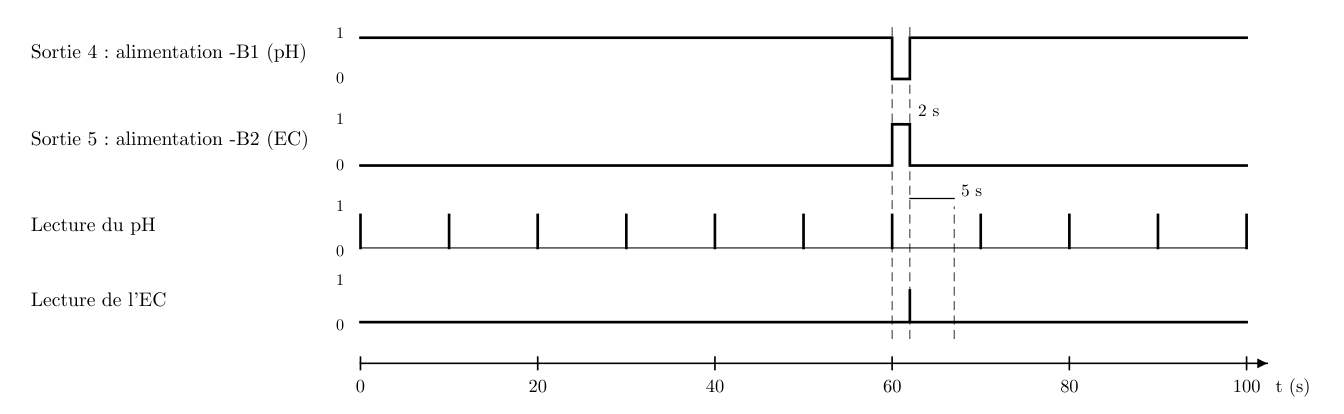
\includegraphics[width=\textwidth]{img/inf/f_chrono_sondes.png}
\caption{Chronogramme : les sondes ne sont jamais alimentées ensemble ; le pH est lu toutes les 10 s, l'EC une fois par minute, et le pH suivant attend 5 s après l'extinction de l'EC.}
\end{figure}

Le script d'essai (partie 8.9) mesure le pH sonde EC éteinte puis allumée : l'écart obtenu montrera sur la vraie tour l'intérêt de cette alternance.

% ---------------------------------------------------------------------
\Needspace{8\baselineskip}\subsection{Programme de l'Arduino}

Une fois l'organisation choisie, il faut donner à l'Arduino un programme qui lui permette d'obéir au Raspberry. Je veux un programme installé une seule fois, qu'on n'ait plus jamais besoin de modifier, mais qui garde une protection si le Raspberry tombe en panne. C'est le seul cas où j'accepte que l'Arduino prenne une décision seul. Cette sous-partie explique le choix de ConfigurableFirmata et les modules activés, puis la sécurité qui coupe les pompes quand le Raspberry ne répond plus.

\subsubsection*{ConfigurableFirmata}

Le projet utilise au départ StandardFirmata, mais cette version ne sait pas lire la sonde de température DS18B20\ix{24}, qui utilise le protocole OneWire. Plutôt que d'écrire un programme Arduino complet, je choisis ConfigurableFirmata : c'est le même protocole, enrichi de modules supplémentaires, dont le OneWire. Je n'active que les modules utiles, pour économiser la mémoire de l'Arduino Uno.

L'Arduino reçoit donc le programme \texttt{HydroTour\_Firmata}, basé sur ConfigurableFirmata. Il active seulement ce qui sert à la tour :

\begin{itemize}
\item les entrées analogiques (capteur de lumière) ;
\item le bus I2C\ix{12} (carte MOSFET\ix{15}, ADS1115\ix{16}, INA260\ix{22}, horloge, Sensor Kit) ;
\item le OneWire (sonde DS18B20\ix{24} sur D2).
\end{itemize}

À la mise en service, la compilation échoue d'abord : la version 3.3 de ConfigurableFirmata renomme une instruction (\texttt{IS\_PIN\_ANALOG} devient \texttt{FIRMATA\_IS\_PIN\_ANALOG}). Une fois corrigé, le programme occupe \qty{12870}{octets} de mémoire programme sur \qty{32256}{octets} (\qty{39,9}{\percent}, car $12870/32256 \approx 0{,}399$) et \qty{884}{octets} de mémoire vive sur \qty{2048}{octets} (\qty{43,2}{\percent}, car $884/2048 \approx 0{,}432$) : il reste de la marge pour l'Arduino Uno.

Le Raspberry s'y connecte à \qty{115200}{bauds}. Il envoie par exemple « écris 0x01 dans le registre 0x12 de la carte 0x20 » pour allumer la pompe principale, ou « lis 2 octets du registre 0x00 de l'ADS1115\ix{16} » pour obtenir une tension.

\subsubsection*{Sécurité : coupure après 30 s de silence}

En me demandant ce qui se passerait si le Raspberry plantait au milieu d'une dose, je vois le risque : la sortie resterait allumée et la doseuse viderait son flacon dans le réservoir, ou la pompe principale tournerait à sec. J'ajoute donc une surveillance dans l'Arduino. Je choisis \qty{30}{s} : c'est assez long pour qu'une mesure un peu lente ne déclenche pas de fausse coupure, et assez court pour arrêter vite une pompe oubliée.

\textbf{Limite.} Cette coupure ne remplace pas une protection locale contre la marche à sec : dans cette version, la décision d'arrêt sur niveau bas est prise par le Raspberry (partie 8.4), et si le Raspberry tombe en panne, la pompe s'arrête après \qty{30}{s} sans pour autant mesurer le niveau. Lire le niveau directement dans l'Arduino est une amélioration prévue (la première version du programme, partie 8.12, le faisait déjà). L'Arduino surveille donc les messages qu'il reçoit :

\begin{itemize}
\item le Raspberry envoie un petit message de présence toutes les \qty{5}{s}, en plus des mesures ;
\item si l'Arduino ne reçoit plus rien pendant \qty{30}{s}, il met les 8 sorties de la carte MOSFET\ix{15} à zéro, puis recommence toutes les \qty{5}{s} tant que le silence dure ;
\item dès que le Raspberry reparle, il renvoie l'état voulu des pompes à chaque mesure : tout repart normalement.
\end{itemize}

Le chronogramme suivant montre la sécurité : sans message du Raspberry pendant \qty{30}{s}, l'Arduino coupe lui-même toutes les sorties.

\begin{figure}[H]
\centering
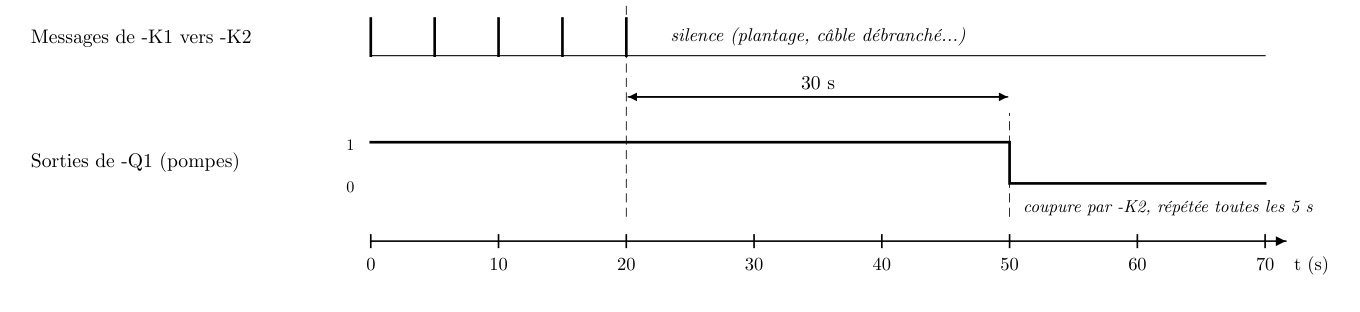
\includegraphics[width=\textwidth]{img/inf/f_chrono_secu.png}
\caption{Chronogramme de la sécurité : sans message de -K1 pendant 30 s, -K2 coupe lui-même toutes les sorties de -Q1.}
\end{figure}


% ---------------------------------------------------------------------
\Needspace{8\baselineskip}\subsection{Programme du Raspberry Pi}

Le Raspberry est le cœur du système : c'est lui qui transforme des tensions en décisions. En écrivant ce programme, je veux pouvoir le tester avant même de recevoir le matériel. Je sépare donc ce qui dépend du matériel de ce qui n'en dépend pas, et je rends réglables depuis le dashboard toutes les valeurs qui risquaient de changer (seuils, durées, étalonnages).

Le programme est écrit en Python et se lance par \texttt{python server.py}. Il est découpé en trois fichiers, chacun avec un rôle clair : \texttt{arduino.py} parle à l'Arduino, \texttt{pilote.py} prend les décisions et \texttt{server.py} relie le tout, enregistre les mesures et sert le dashboard. Le fichier de décisions n'utilise aucun matériel : il peut être testé entièrement sur un ordinateur.

Cette sous-partie suit le trajet d'une mesure dans le programme : la boucle qui mesure et décide toutes les 10 secondes, puis le passage des tensions aux mesures, avec les calculs du pH, de l'EC et du niveau. Elle présente ensuite les décisions : la commande de la pompe principale selon la batterie et le soleil, et le dosage des engrais et du pH$-$ selon le légume. Elle se termine par les alertes et le journal.

\subsubsection*{La boucle de mesure}

Je choisis une période de \qty{10}{s} : c'est assez rapide pour réagir à un réservoir qui se vide, et assez lent pour laisser le temps de lire tous les capteurs (la sonde de température demande à elle seule près d'une seconde). L'ordre des étapes suit le raisonnement d'un jardinier : regarder, comprendre, décider, agir, puis noter ce qui a été fait.

Toutes les 10 secondes, le Raspberry enchaîne les mêmes étapes. Il commence par lire tous les capteurs (avec l'alternance pH / EC de la partie 8.2), puis il convertit les tensions en valeurs physiques (pH, \unit{\micro S/cm}, \%) avec l'étalonnage. Ensuite il calcule les cibles de pH et d'EC du légume, selon son stade, puis il décide de la pompe principale et des doses (parties 8.4, pompe principale et dosage). Enfin il renvoie l'état des pompes à l'Arduino, enregistre la mesure dans la base et met à jour l'écran.

Une erreur sur un capteur (fil débranché, module absent) n'arrête pas la boucle : la valeur manque simplement, et le module absent n'est réinterrogé qu'une minute plus tard pour ne pas ralentir les autres mesures.

\subsubsection*{Des tensions aux mesures}

Les capteurs ne donnent pas directement un pH ou une conductivité, mais une tension. Je reprends les formules des fabricants, et je place tous les réglages d'étalonnage dans le dashboard plutôt que dans le code : une sonde pH dérive avec le temps, et il faut pouvoir la réétalonner sans ouvrir le programme. Les capteurs analogiques donnent une tension ; le programme la transforme en grandeur utile. Les exemples ci-dessous reprennent les valeurs affichées dans les captures de la partie 8.5.

\naturecalc{théorie (formule démontrée, valeurs de fiches techniques et hypothèses ; rien de mesuré)}
\begin{demonstration}[pH à partir de la tension]
\resultat{\mathrm{pH} \approx 5{,}97}
La sonde est étalonnée dans deux solutions tampon : $U_7 = \qty{1500}{mV}$ à pH 7 et $U_4 = \qty{2032}{mV}$ à pH 4. J'admets que le pH est une fonction affine de la tension $U$ lue, en millivolts :
\[
\mathrm{pH} = a\,U + b
\]
Les deux solutions tampon donnent deux équations :
\begin{align*}
7 &= a\,U_7 + b\\
4 &= a\,U_4 + b
\end{align*}
En soustrayant la seconde à la première, $b$ disparaît :
\begin{align*}
7 - 4 &= a\,(U_7 - U_4)\\
a &= \frac{4-7}{U_4 - U_7}
\end{align*}
Je remplace $b$ en utilisant la première équation, $b = 7 - a\,U_7$ :
\begin{align*}
\mathrm{pH} &= a\,U + 7 - a\,U_7\\
\mathrm{pH} &= 7 + (U - U_7)\times\frac{4-7}{U_4 - U_7}
\end{align*}
Pour $U = \qty{1683}{mV}$ :
\begin{align*}
U_4 - U_7 &= \qty{2032}{mV} - \qty{1500}{mV} = \qty{532}{mV}\\
\mathrm{pH} &= 7 + (\qty{1683}{mV} - \qty{1500}{mV})\times\frac{-3}{\qty{532}{mV}}\\
\mathrm{pH} &= 7 - \frac{\qty{183}{mV}\times 3}{\qty{532}{mV}}\\
\mathrm{pH} &= 7 - 1{,}03\\
\mathrm{pH} &\approx 5{,}97
\end{align*}
Le résultat est arrondi au centième.
\end{demonstration}

\naturecalc{théorie (formule démontrée, valeurs de fiches techniques et hypothèses ; rien de mesuré)}
\begin{demonstration}[conductivité ramenée à \qty{25}{\celsius}]
\resultat{\mathrm{EC}_{25} \approx \qty{1467}{\micro S/cm}}
La conductivité d'une eau est la conductance mesurée entre deux électrodes, multipliée par la constante de cellule $K$ de la sonde (en cm$^{-1}$, rapport de la distance entre électrodes à leur surface). Cet exemple reprend la sonde du système de départ, la DFR0300 (la formule de la sonde fabriquée est en partie 7.7). La carte de la sonde DFR0300 transforme cette conductance en une tension $U$ proportionnelle. La conductivité brute est donc proportionnelle à $U$ et à $K$. Pour cette carte, le constructeur donne le coefficient de proportionnalité $\dfrac{1000}{820 \times 200}$, avec $U$ en millivolts et $K = 1$ :
\[
\mathrm{EC} = \frac{1000 \times U}{820 \times 200}\times K
\]
La conductivité augmente avec la température $T$ de l'eau (en \unit{\celsius}). J'admets une variation affine de $\alpha = \qty{1,85}{\percent}$ par degré (valeur du programme du dashboard ; la partie 7 prend \qty{2}{\percent}, valeur usuelle : l'écart de \qty{0,15}{\percent} par degré change l'EC de moins de \qty{1}{\percent} pour \qty{3}{\celsius} d'écart avec \qty{25}{\celsius}, sans effet sur le dosage) autour de \qty{25}{\celsius} :
\[
\mathrm{EC} = \mathrm{EC}_{25}\,\bigl[1 + \alpha\,(T - 25)\bigr]
\]
En isolant $\mathrm{EC}_{25}$, la conductivité ramenée à \qty{25}{\celsius}, on obtient :
\[
\mathrm{EC}_{25} = \frac{\mathrm{EC}}{1 + 0{,}0185\,(T - 25)}
\]
Pour $U = \qty{229}{mV}$ et $T = \qty{22,4}{\celsius}$ :
\begin{align*}
\mathrm{EC} &= \frac{1000 \times 229}{820 \times 200}\ \unit{mS/cm} = \frac{229000}{164000}\ \unit{mS/cm}\\
\mathrm{EC} &\approx \qty{1,396}{mS/cm}\\
1 + 0{,}0185 \times (22{,}4 - 25) &= 1 - 0{,}0481 = 0{,}9519\\
\mathrm{EC}_{25} &= \frac{\qty{1,396}{mS/cm}}{0{,}9519}\\
\mathrm{EC}_{25} &\approx \qty{1,467}{mS/cm} = \qty{1467}{\micro S/cm}
\end{align*}
\end{demonstration}

\naturecalc{théorie (formule démontrée, valeurs de fiches techniques et hypothèses ; rien de mesuré)}
\begin{demonstration}[niveau du réservoir]
\resultat{\text{niveau} = \qty{77,5}{\percent}\ \text{pour}\ R = \qty{760}{\ohm}}
Le ruban eTape\ix{23} est une résistance $R$ (en ohms) qui diminue quand l'eau monte. Il est placé en série avec une résistance de \qty{560}{\ohm}, sous \qty{5}{V} (\qty{5000}{mV}) : la tension $U$ lue entre les deux (en millivolts) est celle aux bornes du ruban. C'est un pont diviseur :
\[
U = 5000 \times \frac{R}{R + 560}
\]
Je multiplie par $R + 560$, puis je regroupe les termes en $R$ :
\begin{align*}
U\,(R + 560) &= 5000\,R\\
560\,U &= 5000\,R - U\,R\\
560\,U &= R\,(5000 - U)\\
R &= 560 \times \frac{U}{5000 - U}
\end{align*}
Le niveau $N$ est ensuite placé entre les deux étalonnages, $R_{\mathrm{vide}} = \qty{2000}{\ohm}$ (réservoir vide, $0\,\%$) et $R_{\mathrm{plein}} = \qty{400}{\ohm}$ (réservoir plein, $100\,\%$). J'admets que le niveau est affine en $R$ : il vaut $100\,\%$ quand $R = R_{\mathrm{plein}}$ et $0\,\%$ quand $R = R_{\mathrm{vide}}$, d'où :
\[
N = \frac{R_{\mathrm{vide}} - R}{R_{\mathrm{vide}} - R_{\mathrm{plein}}}\times 100
\]
Pour $R = \qty{760}{\ohm}$ :
\begin{align*}
N &= \frac{\qty{2000}{\ohm} - \qty{760}{\ohm}}{\qty{2000}{\ohm} - \qty{400}{\ohm}}\times 100\\
N &= \frac{\qty{1240}{\ohm}}{\qty{1600}{\ohm}}\times 100\\
N &= \qty{77,5}{\percent}
\end{align*}
Le tableau de l'étude de départ arrondit à \qty{77}{\percent} ; c'est la valeur affichée sur les captures.
\end{demonstration}

Les valeurs d'étalonnage (tensions du pH, résistances vide et plein) s'enregistrent d'un bouton dans le dashboard, sans toucher au code.

\subsubsection*{La pompe principale}

Pour la pompe principale, je pars de la consommation : avec \qty{19}{W}, c'est l'appareil qui consomme le plus. Quand la batterie baisse, c'est donc elle qu'il faut arrêter en premier, pour garder le Raspberry allumé et continuer à mesurer. Un seul seuil ferait clignoter la pompe, car la tension de la batterie remonte dès qu'on coupe la charge : je choisis donc deux seuils, l'un pour couper, l'autre pour reprendre. Enfin, il serait dommage d'attendre \qty{35}{\percent} alors que le soleil recharge déjà largement la batterie. J'ajoute une reprise anticipée qui exige à la fois du courant de charge et de la lumière, pour ne pas se tromper sur une seule mesure.

En temps normal, la pompe suit un cycle réglable (\qty{15}{min} de marche, \qty{15}{min} d'arrêt par défaut).

Ce cycle vaut pour la journée, de 6 h à 18 h. La nuit, la pompe ne fait que trois marches de \qty{15}{min}, à 21 h, 0 h et 3 h. C'est le planning de l'étude électrique (partie 5) : \qty{6}{h} de marche le jour et \qty{0,75}{h} la nuit, soit \qty{6,75}{h} par jour, ce qui donne le bilan de \qty{226,7}{Wh/j}.

Deux sécurités peuvent arrêter la pompe :

\begin{itemize}
\item le réservoir presque vide (moins de \qty{15}{\percent}) : la pompe ne doit pas tourner à sec ;
\item la batterie basse : la pompe consomme \qty{19}{W}, c'est elle qu'on sacrifie en premier pour garder le Raspberry allumé.
\end{itemize}

Le seuil de coupure et le seuil de reprise se règlent dans le dashboard. On conseille de couper à \qty{30}{\percent} et de reprendre à \qty{35}{\percent} : l'écart de \qty{5}{\percent} évite que la pompe s'allume et s'éteigne sans arrêt autour d'un seul seuil. Si un réglage plus bas est choisi, le dashboard affiche un conseil. Ces seuils sont des paramètres de pilotage, pas des valeurs validées par un essai. Le pourcentage est déduit de la tension lue par l'INA260\ix{22} ; il dépend de la technologie de la batterie (en LiFePO4, la tension varie très peu sur presque toute la décharge) et la tension baisse sous charge. Il faut donc relever la courbe tension-charge de la vraie batterie, au repos et pendant la marche de la pompe, avant de se fier à ces pourcentages.

La pompe peut aussi repartir avant \qty{35}{\percent} s'il y a assez de soleil : quand le panneau recharge la batterie d'au moins \qty{1,5}{A} (de quoi alimenter la pompe) et que la lumière dépasse \qty{60}{\percent}, pendant 5 minutes. Si le soleil disparaît pendant 2 minutes, elle s'arrête de nouveau.

Je décris ce comportement par un GRAFCET (norme IEC 60848), l'outil habituel pour représenter un automatisme : chaque étape (carré numéroté) correspond à un état de la pompe, avec son action à droite, et on ne passe d'une étape à la suivante que si la réceptivité écrite à côté de la transition (petit trait horizontal) est vraie. La condition « $N \geq \qty{15}{\percent}$ » au-dessus des actions traduit l'arrêt de la pompe quand le réservoir est presque vide, quelle que soit l'étape.

\begin{figure}[H]
\centering
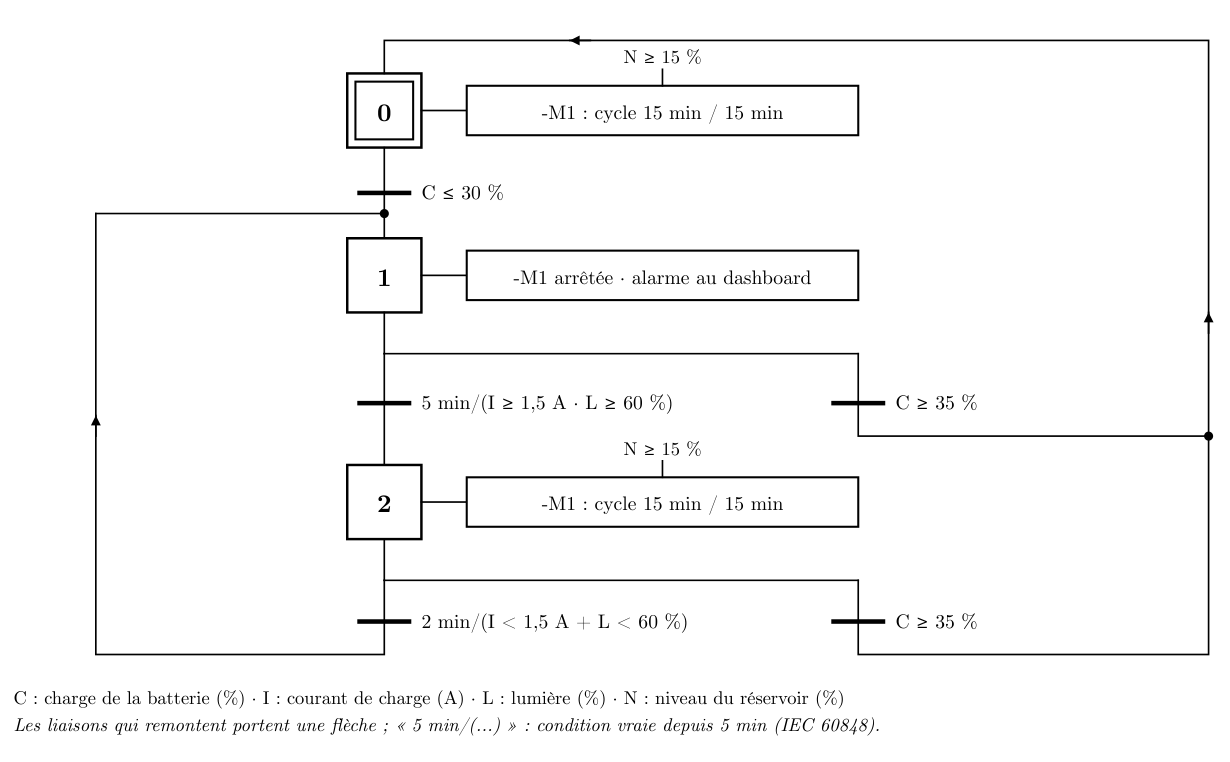
\includegraphics[width=0.9\textwidth]{img/inf/f_grafcet.png}
\schemacap{grafcet}{GRAFCET (IEC 60848) de la pompe principale -M1 : étape 0 normale, étape 1 coupée, étape 2 relancée par le soleil. Les seuils de 30 \% et 35 \% sont les valeurs conseillées, réglables dans le dashboard.}
\end{figure}

\subsubsection*{Le dosage selon le légume}

Pour le dosage, je veux éviter deux erreurs : verser trop de produit d'un coup, et corriger de nouveau avant que l'eau soit mélangée. Je choisis donc des doses courtes suivies d'une attente, comme on le ferait à la main. Les cibles changent avec le légume et son âge : plutôt que de les recopier dans le programme, je fais relire au Raspberry le tableau du dashboard, pour qu'il n'existe qu'une seule liste. Les essais me montrent aussi qu'il faut alterner engrais et pH$-$ quand les deux sont hors cible.

Les cibles de pH et d'EC dépendent du légume et de son stade de croissance, compté en jours depuis la plantation. Le tableau des légumes est écrit une seule fois, dans le dashboard ; le Raspberry le relit au démarrage, ce qui évite d'avoir deux listes différentes.

\begin{table}[H]
\centering
\small
\begin{tabularx}{\textwidth}{|l|l|c|c|}
\hline
\textbf{Légume} & \textbf{Stade (jours)} & \textbf{pH cible} & \textbf{EC cible (\unit{\micro S/cm})} \\
\hline
Salade (laitue) & Reprise (0--5) & 5,6 -- 6,0 & 1000 -- 1200 \\
 & Croissance des feuilles (5--22) & 5,6 -- 6,0 & 1200 -- 1600 \\
 & Pommaison (22--32) & 5,6 -- 6,0 & 1400 -- 1800 \\
 & Prête à récolter (32--42) & 5,6 -- 6,0 & 1400 -- 1800 \\
\hline
Tomate (cerise) & Reprise (0--7) & 5,8 -- 6,2 & 1500 -- 2000 \\
 & Croissance végétative (7--21) & 5,8 -- 6,2 & 1800 -- 2200 \\
 & Floraison (21--35) & 5,8 -- 6,3 & 2000 -- 2400 \\
 & Grossissement des fruits (35--60) & 5,8 -- 6,3 & 2200 -- 2800 \\
 & Récolte continue (60--88) & 5,8 -- 6,5 & 2400 -- 3000 \\
\hline
Poivron & Reprise (0--10) & 5,8 -- 6,2 & 1500 -- 1800 \\
 & Croissance végétative (10--30) & 5,8 -- 6,2 & 1800 -- 2200 \\
 & Floraison (30--45) & 5,8 -- 6,3 & 2000 -- 2300 \\
 & Grossissement des fruits (45--75) & 5,8 -- 6,3 & 2200 -- 2500 \\
 & Récolte (75--103) & 5,8 -- 6,3 & 2200 -- 2500 \\
\hline
\end{tabularx}
\caption{Cibles de pH et d'EC selon le légume et son stade.}
\end{table}

Les doses sont petites et espacées, pour laisser à l'eau le temps de se mélanger avant de mesurer à nouveau :

\begin{itemize}
\item on ne dose que si la pompe principale tourne depuis au moins 2 min (l'eau circule) et si le réservoir n'est pas presque vide ;
\item on attend \qty{10}{min} entre deux doses ;
\item EC trop basse : \qty{3}{s} d'engrais A, puis \qty{3}{s} d'engrais B ;
\item pH trop haut : \qty{2}{s} de pH$-$ ;
\item l'EC passe d'abord, car les engrais font bouger le pH ; si les deux sont hors cible, on alterne ;
\item au plus 12 doses par jour et par produit : au-delà, une sonde est sûrement défaillante.
\end{itemize}

L'organigramme suivant décrit le dosage, à chaque mesure.

\begin{figure}[H]
\centering
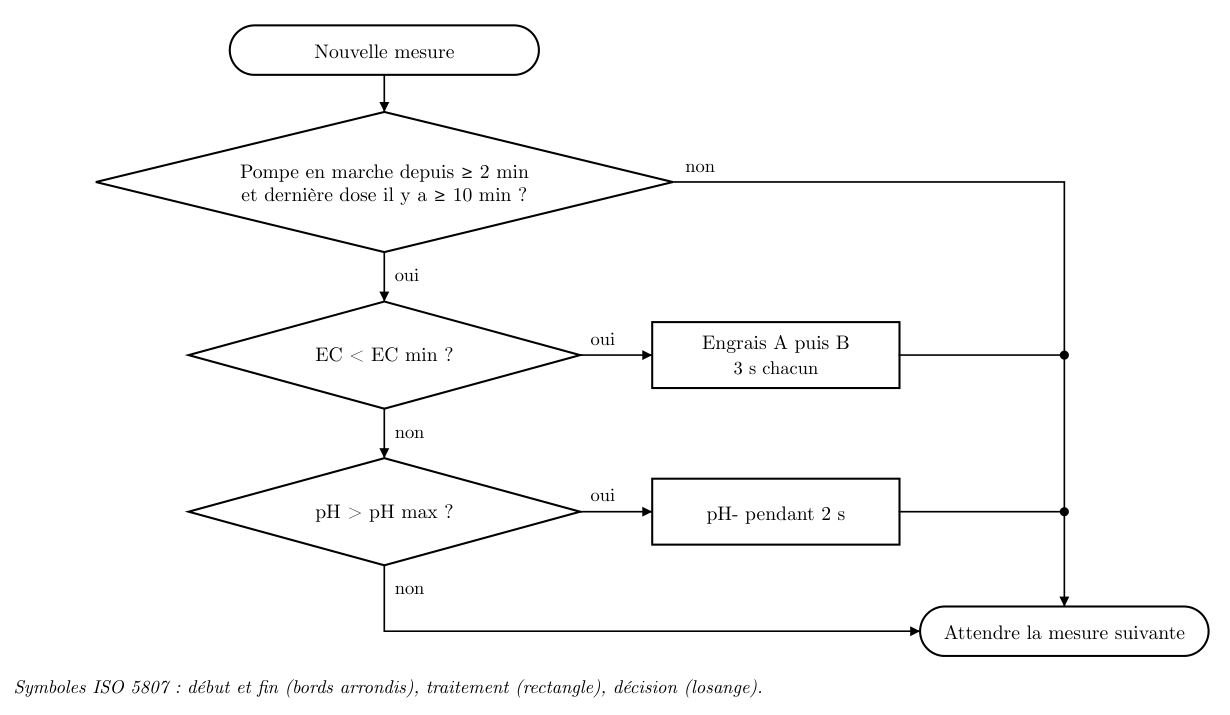
\includegraphics[width=0.85\textwidth]{img/inf/f_organigramme.png}
\schemacap{organi}{Organigramme (ISO 5807) du dosage, à chaque mesure. Pour rester lisible, il ne montre ni l'alternance entre engrais et pH$-$, ni la limite de 12 doses par jour.}
\end{figure}

\naturecalc{théorie (formule démontrée, valeurs de fiches techniques et hypothèses ; rien de mesuré)}
\begin{demonstration}[volume d'une dose]
\resultat{V_{\mathrm{engrais}} \approx \qty{5}{mL}\ \text{au plus}, \quad V_{\mathrm{pH-}} \approx \qty{3,3}{mL}\ \text{au plus}}
Les pompes péristaltiques\ix{8} débitent au plus $Q = \qty{100}{mL/min}$ (valeur de la fiche, à vide). Je calcule donc ici le volume maximal d'une dose. En divisant par $\qty{60}{s/min}$ :
\begin{align*}
Q &= \frac{\qty{100}{mL}}{\qty{60}{s}}\\
Q &\approx \qty{1,67}{mL/s}
\end{align*}
Le débit est constant : le volume versé pendant une durée $t$ (en secondes) est le produit du débit par la durée :
\[
V = Q \times t
\]
Pour chaque engrais, $t = \qty{3}{s}$ :
\begin{align*}
V &= \qty{1,67}{mL/s}\times\qty{3}{s}\\
V &\approx \qty{5}{mL}
\end{align*}
Pour le pH$-$, $t = \qty{2}{s}$ :
\begin{align*}
V &= \qty{1,67}{mL/s}\times\qty{2}{s}\\
V &\approx \qty{3,3}{mL}
\end{align*}
Le programme retire ces volumes du stock d'engrais saisi dans le dashboard, pour prévenir quand un flacon se vide. Ce sont des valeurs maximales : avec le débit en charge de \qty{80}{mL/min} supposé dans l'étude électrique (partie 5), une dose de \qty{3}{s} verse environ \qty{4}{mL} et une dose de \qty{2}{s} environ \qty{2,7}{mL}. La mesure M5 (partie 5) donnera le débit réel.
\end{demonstration}

\subsubsection*{Alertes et journal}

Un système autonome doit savoir prévenir quand il ne peut plus agir seul : réservoir vide, flacon d'engrais épuisé, pH trop bas alors qu'il n'y a pas de pH$+$. Je sépare les alarmes, qui demandent une action rapide, des simples avertissements, pour qu'on ne s'habitue pas à ignorer les messages rouges. À chaque mesure, le pilote dresse la liste des problèmes en cours. Les alarmes (en rouge) sont aussi notées dans le journal, avec les doses et les changements d'état :

\begin{table}[H]
\centering
\small
\begin{tabularx}{\textwidth}{|Y|l|Y|}
\hline
\textbf{Situation} & \textbf{Niveau} & \textbf{Message affiché} \\
\hline
Batterie sous le seuil de coupure & alarme & pompe arrêtée, reprise à \qty{35}{\percent} ou au soleil \\
\hline
Réservoir sous \qty{15}{\percent} & alarme & pompe et dosage arrêtés, ajouter de l'eau \\
\hline
12 doses dans la journée & alarme & dosage bloqué jusqu'au lendemain, vérifier la sonde \\
\hline
pH trop bas & à surveiller & pas de pH$+$ : corriger à la main \\
\hline
EC trop haute & à surveiller & ajouter de l'eau claire \\
\hline
Stock d'engrais sous \qty{0,2}{L} & à surveiller & flacon presque vide \\
\hline
Coupure sous \qty{30}{\percent} ou reprise sous \qty{35}{\percent} & conseil & valeurs conseillées pour protéger la batterie \\
\hline
Mode manuel & à surveiller & pilotage automatique en pause \\
\hline
\end{tabularx}
\caption{Alertes du pilote.}
\end{table}


% ---------------------------------------------------------------------
\Needspace{8\baselineskip}\subsection{Le dashboard}

Le dashboard existe déjà pour afficher les mesures. Je le complète pour qu'il devienne le poste de commande du pilotage : la tour n'a ni clavier ni grand écran, et je veux pouvoir tout régler depuis un téléphone. Je veux aussi comprendre à tout moment pourquoi la tour a agi, d'où l'importance des alertes et du journal.

Le dashboard est une page web servie par le Raspberry, à l'adresse \texttt{http://<ip-du-raspberry>:5000}. On l'ouvre depuis n'importe quel téléphone ou ordinateur du même réseau Wi-Fi ; elle se met à jour toutes les 10 secondes. Les captures ci-dessous sont faites avec un Arduino simulé (partie 8.9) ; l'accès depuis Internet et sa page de connexion sont présentés dans la partie 8.6. Cette sous-partie présente le dashboard onglet par onglet : d'abord les mesures, puis la tour en 3D et la commande manuelle des pompes, et enfin les réglages du pilotage et l'étalonnage des sondes.

\subsubsection*{Les mesures}

Sur l'onglet Mesures, je veux qu'on voie en un coup d'œil si tout va bien. Chaque mesure est comparée à la cible du légume, et les alertes du Raspberry s'ajoutent au bandeau du haut. J'ajoute aussi la pression, et j'affiche la lumière en pourcentage : le capteur du Sensor Kit n'est pas étalonné, et afficher des lux serait trompeur.

\begin{figure}[H]
\centering
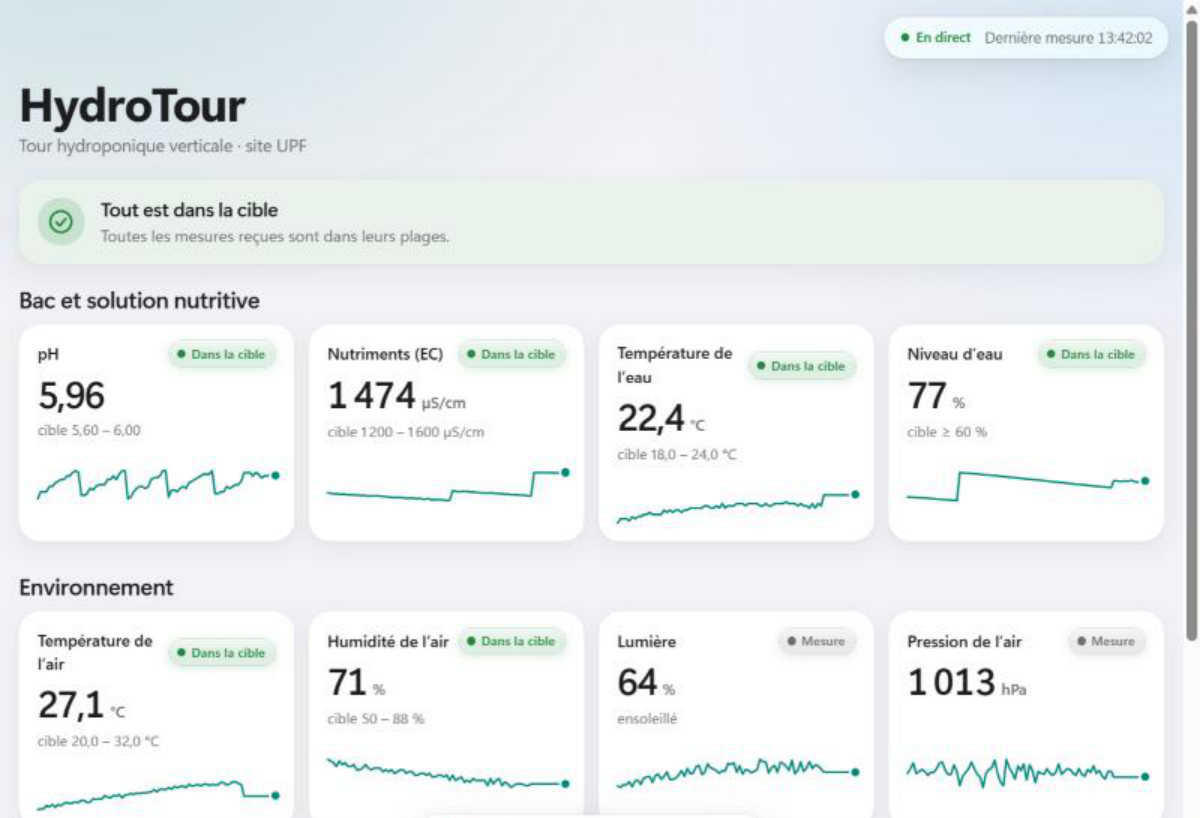
\includegraphics[width=\textwidth]{img/inf/d_mesures.png}
\caption{Onglet Mesures : chaque tuile indique la valeur, la cible du légume et la courbe des 6 dernières heures. Le bandeau du haut résume l'état et affiche les alertes du pilote.}
\end{figure}

\subsubsection*{La tour et les pompes}

La commande manuelle reste indispensable pour les essais et l'entretien. Je décide qu'un appui manuel sur la circulation mette l'automatique en pause : sinon, le Raspberry rallumerait la pompe dix secondes plus tard, et on ne comprendrait pas pourquoi. Je retire la pompe d'eau claire de l'affichage sur la vraie tour, puisqu'elle n'existe que dans la démonstration.

La figure suivante montre l'onglet Installation du dashboard.

\begin{figure}[H]
\centering
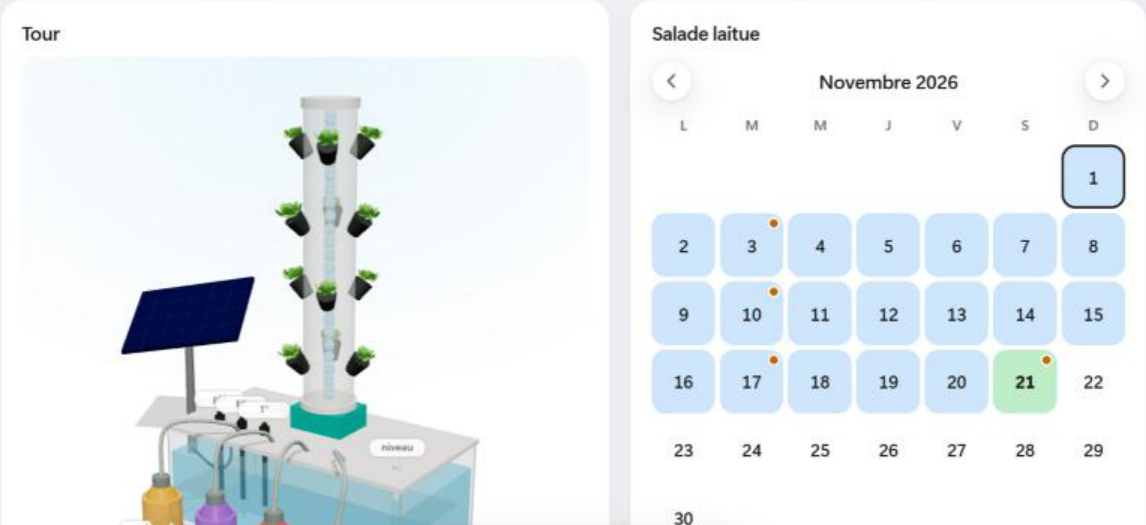
\includegraphics[width=\textwidth]{img/inf/d_tour.png}
\caption{Onglet Installation : la tour en 3D suit le stade du légume, et le calendrier rappelle les contrôles à faire.}
\end{figure}

La carte des pompes montre l'état de chacune. Le bouton Arrêter / Démarrer commande la circulation à la main : le pilotage automatique se met alors en pause, jusqu'à ce qu'on le réactive dans les paramètres. Les boutons Doser 3 s lancent une dose manuelle. Le stock d'engrais restant est rappelé sous chaque doseuse.

La figure suivante montre la carte des pompes.

\begin{figure}[H]
\centering
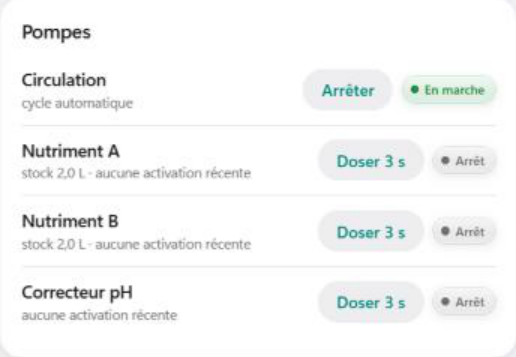
\includegraphics[width=0.6\textwidth]{img/inf/d_pompes.png}
\caption{Carte des pompes.}
\end{figure}

\subsubsection*{Les paramètres}

Les seuils de batterie conseillés ne conviennent pas forcément à toutes les situations : je choisis donc de les laisser réglables, tout en affichant un conseil quand on descend sous \qty{30}{\percent} ou \qty{35}{\percent}. Le serveur vérifie aussi les valeurs reçues, pour qu'une erreur de saisie ne puisse pas bloquer la pompe.

La figure suivante montre les réglages du pilotage et l'étalonnage.

\begin{figure}[H]
\centering
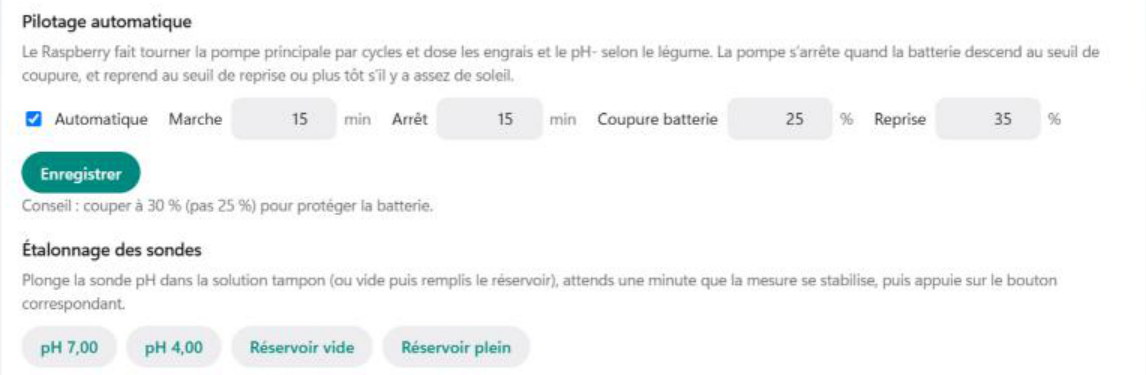
\includegraphics[width=\textwidth]{img/inf/d_param.png}
\caption{Réglages du pilotage et étalonnage. Avec une coupure à 25 \%, le dashboard conseille de couper à 30 \%.}
\end{figure}

Le bloc Pilotage automatique règle le cycle de la pompe et les seuils de la batterie ; le serveur refuse une reprise trop proche de la coupure. Le bloc Étalonnage des sondes enregistre la mesure du moment comme référence : pH 7 et pH 4 dans les solutions tampon, réservoir vide et plein. Le choix du légume et de sa date de plantation est envoyé au Raspberry, qui adapte aussitôt ses cibles. Enfin, le bloc Accès, en haut des paramètres, permet de changer l'identifiant et le mot de passe du site et de se déconnecter (partie 8.6).

% ---------------------------------------------------------------------
\Needspace{8\baselineskip}\subsection{Accès à distance et sécurité}

Jusqu'ici, le dashboard ne s'ouvre que depuis le Wi-Fi de la maison. Or la tour doit tourner seule pendant des jours : je veux pouvoir vérifier le pH ou la batterie depuis l'université, et réagir à une alarme sans être sur place. Mettre la tour sur Internet pose une nouvelle question : comment empêcher n'importe qui de commander les pompes ? Je cherche une solution gratuite, simple à installer sur le Raspberry, et qui ne m'oblige pas à toucher aux réglages de la box.

Cette sous-partie explique le choix de Tailscale\ix{20} Funnel\ix{20} pour rendre la tour joignable depuis Internet, puis la première version de la protection, trop compliquée, et la solution simple que je retiens. Elle présente ensuite la page de connexion, avec son identifiant, son mot de passe et son captcha, et se termine par les deux portes d'entrée du serveur et ce qui est protégé.

\subsubsection*{Rendre la tour joignable depuis Internet}

Le Raspberry est branché derrière la box de la maison : depuis Internet, on ne peut pas l'atteindre directement. Je compare trois solutions :

\begin{table}[H]
\centering
\small
\begin{tabularx}{\textwidth}{|l|Y|Y|}
\hline
\textbf{Solution} & \textbf{Avantages} & \textbf{Inconvénients} \\
\hline
Ouvrir un port de la box & aucun service extérieur & le Raspberry est exposé directement ; dépend de la box et de l'opérateur ; certificat https à gérer soi-même \\
\hline
Cloudflare Tunnel & gratuit, https, rien à ouvrir sur la box & demande un nom de domaine payant (environ 10 euros par an) pour une adresse fixe \\
\hline
Tailscale\ix{20} Funnel\ix{20} (retenu) & gratuit, https, adresse fixe en \texttt{.ts.net}, rien à ouvrir sur la box & dépend du service Tailscale\ix{20} \\
\hline
\end{tabularx}
\caption{Comparaison des trois solutions d'accès depuis Internet.}
\end{table}

Je retiens Tailscale\ix{20} Funnel\ix{20}. Un petit programme installé sur le Raspberry ouvre lui-même une connexion vers Tailscale\ix{20} ; les visiteurs passent par Tailscale\ix{20}, qui leur fournit le https et transmet leurs demandes au Raspberry. La box ne voit qu'une connexion sortante, comme pour n'importe quel site visité. L'adresse publique ne change jamais, et une seule commande suffit pour publier le serveur : \texttt{sudo tailscale funnel --bg 5001}.

\subsubsection*{Une première version trop compliquée}

Je conçois d'abord une gestion complète des comptes : un compte administrateur qui crée des comptes lecteurs, chacun avec son identifiant, son mot de passe et son adresse mail ; des mots de passe provisoires à changer à la première connexion ; et un lien de réinitialisation envoyé par mail, valable 15 minutes. Avant de l'écrire, j'évalue ce qu'elle demande : une base des comptes, une page d'administration, l'envoi de mails par le Gmail du projet\ldots{} J'en écris et j'en teste une première version.

En la reprenant, je me rends compte qu'elle est disproportionnée : la tour n'a que quelques utilisateurs, qui se connaissent tous. J'annule donc tout au profit d'une solution simple : un seul identifiant et un seul mot de passe, partagés. Quiconque les connaît a tous les droits. Le prix de cette simplicité est connu : on ne sait pas qui a fait quoi, et pour retirer l'accès à quelqu'un, il faut changer le mot de passe de tout le monde. Pour ce projet, ce compromis me paraît raisonnable.

\subsubsection*{La page de connexion}

Toute visite commence par une page de connexion, aussi bien depuis Internet que depuis le Wi-Fi de la maison : un invité branché sur le Wi-Fi ne doit pas pouvoir commander les pompes. La page demande trois choses : l'identifiant, le mot de passe et un captcha.

La figure suivante montre la page de connexion, avec son captcha.

\begin{figure}[H]
\centering
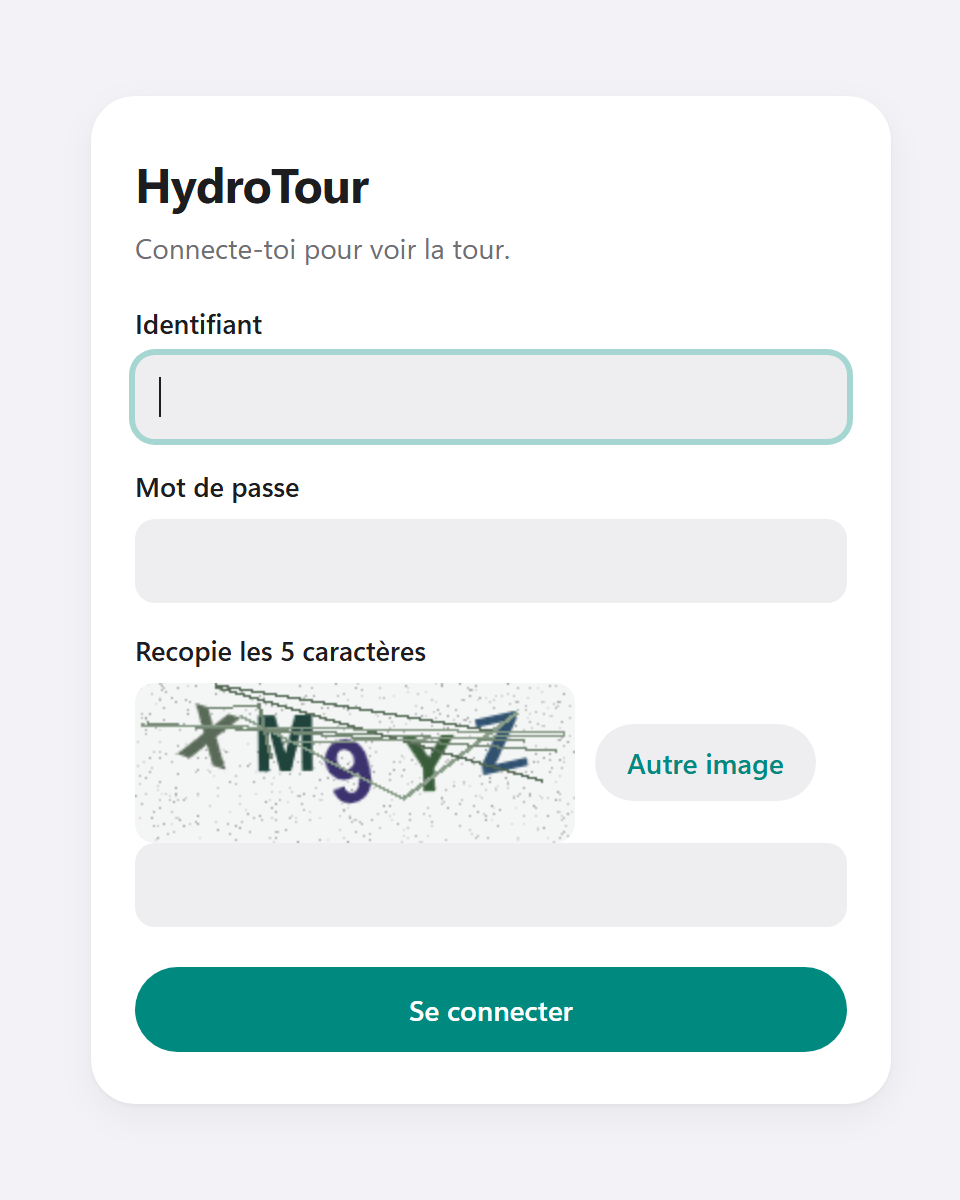
\includegraphics[width=0.5\textwidth]{img/inf/d_login.png}
\caption{La page de connexion, avec son captcha.}
\end{figure}

Le captcha est fait maison : le Raspberry dessine une image de cinq caractères penchés, de couleurs différentes, barrés de traits, avec la bibliothèque Pillow déjà utilisée pour l'écran. Je retire les caractères qui se confondent (0 et O, 1, I et L). Chaque image ne sert qu'une seule fois et expire au bout de 10 minutes : un robot ne peut pas réutiliser une réponse trouvée une fois. Le nombre d'essais n'est pas limité : c'est un choix volontaire, le captcha suffisant à ralentir un robot qui essaierait des mots de passe au hasard.

\begin{itemize}
\item \textbf{Mot de passe protégé} : il n'est jamais enregistré en clair, seulement son empreinte (hachage scrypt) ; même en lisant la base de données, on ne peut pas le retrouver.
\item \textbf{Premier lancement} : le serveur crée l'identifiant \texttt{hydrotour} avec un mot de passe provisoire, affiché sur le Raspberry et écrit dans un fichier qui s'efface dès qu'on le change.
\item \textbf{Changement} : dans Paramètres $>$ Accès, en redonnant l'ancien mot de passe. Tous les autres appareils sont alors déconnectés.
\item \textbf{Session} : on reste connecté 30 jours, ou jusqu'au bouton « Se déconnecter ».
\item \textbf{Oubli} : sur le Raspberry, la commande \texttt{python acces.py secours} crée un nouveau mot de passe provisoire.
\end{itemize}

\subsubsection*{Deux portes d'entrée}

En préparant la protection, je rencontre une difficulté : Tailscale\ix{20} transmet les visites d'Internet au Raspberry depuis le Raspberry lui-même (adresse 127.0.0.1). Pour le serveur, un visiteur venu d'Internet ressemble donc à un appareil de la maison. Or certaines demandes ne doivent venir que de la maison, comme \texttt{/api/data}, par laquelle un ancien Arduino Wi-Fi envoie ses mesures sans mot de passe. Je résous le problème en donnant au serveur deux portes :

Le schéma suivant montre les deux portes d'entrée du serveur et la règle commune.

\begin{figure}[H]
\centering
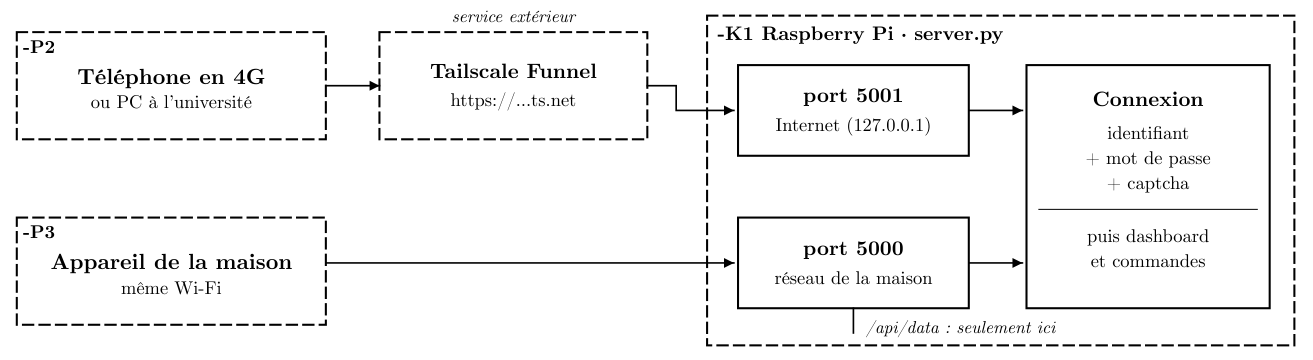
\includegraphics[width=\textwidth]{img/inf/f_portes.png}
\caption{Deux portes d'entrée, une seule règle : il faut se connecter. Seule la porte de la maison accepte aussi les mesures envoyées sans mot de passe.}
\end{figure}

La porte 5001 n'écoute que sur le Raspberry lui-même : seul Tailscale\ix{20} peut l'utiliser, et tout ce qui y arrive est traité comme venant d'Internet. La porte 5000 sert le réseau de la maison. Les deux demandent la connexion ; seule la porte 5000 accepte en plus \texttt{/api/data}, et seulement depuis une adresse locale. Je retire aussi une autorisation qui laisse n'importe quel site lire les mesures (en-tête CORS « $*$ »), et j'interdis l'affichage du dashboard à l'intérieur d'un autre site.

\begin{aretenir}
Sans connexion, seules la page de connexion et l'image du captcha répondent ; toute autre demande est renvoyée vers la connexion. Je vérifie chaque cas par des essais automatiques (23 cas : mauvais captcha, captcha réutilisé, mauvais mot de passe, déconnexion des autres appareils\ldots), puis depuis l'adresse publique : \texttt{/api/data} y est bien refusée.
\end{aretenir}

% ---------------------------------------------------------------------
\Needspace{8\baselineskip}\subsection{Mise en service sur le matériel}

Depuis le 1er novembre, une partie du matériel est enfin disponible : l'Arduino Uno et son Sensor Kit, l'horloge et la sonde pH, branchés au Raspberry. C'est le moment de vérifier que le programme, testé jusque-là avec un Arduino simulé, fonctionne vraiment. J'avance pas à pas, en contrôlant chaque étape avant de passer à la suivante, et je note chaque problème rencontré avec sa cause.

Cette sous-partie suit la mise en service dans l'ordre : l'installation du programme de l'Arduino, sans le débrancher du Raspberry, puis celle du serveur sur le Raspberry. Elle présente ensuite le script de diagnostic et ce qu'il trouve, les défauts découverts et leur correction, et enfin ce qu'affiche maintenant l'écran de la tour.

\subsubsection*{Installer le programme de l'Arduino}

L'Arduino est branché au Raspberry, qui n'a pas l'environnement Arduino. Plutôt que de le débrancher, je compile le programme sur l'ordinateur avec l'outil en ligne de commande de l'IDE Arduino (\texttt{arduino-cli}), ce qui révèle l'erreur de compilation décrite dans la partie 8.3. Le fichier obtenu (\texttt{HydroTour\_Firmata\_uno.hex}) est copié sur le Raspberry, puis téléversé dans l'Arduino par le port USB avec l'outil \texttt{avrdude}.

Il faut d'abord arrêter l'ancien programme \texttt{pont\_usb.py}, qui tourne encore sur le Raspberry et occupe le port USB de l'Arduino. Dans la nouvelle organisation, c'est le serveur qui parle directement à l'Arduino : ce pont est donc désactivé pour de bon.

\subsubsection*{Installer le serveur sur le Raspberry}

Les fichiers du dossier \texttt{SERVEUR} sont copiés depuis l'ordinateur, à travers Tailscale\ix{20}, avec la commande \texttt{scp}. Deux surprises apparaissent :

\begin{itemize}
\item \textbf{Installer des bibliothèques Python} : le système du Raspberry (Debian 13) refuse \texttt{pip install}, pour ne pas abîmer son propre Python. Flask et Pillow existent en paquets du système (\texttt{apt}) ; \texttt{pyfirmata2} non. Je l'installe donc dans un environnement virtuel (\texttt{venv}), un dossier qui garde ses propres bibliothèques tout en voyant celles du système.
\item \textbf{Lancer le serveur au démarrage} : un service du système (\texttt{hydrotour.service}) lance le serveur avec le Python du \texttt{venv} et le relance s'il s'arrête. J'ajoute l'option \texttt{-u} : sans elle, les messages du serveur restent en mémoire au lieu d'apparaître dans le journal du système, ce qui empêche de suivre ce qu'il fait.
\end{itemize}

\subsubsection*{Un script de diagnostic}

Au premier démarrage, rien ne s'affiche sur l'écran et plusieurs mesures manquent. Plutôt que de deviner, j'écris un court script, \texttt{diagnostic.py}, qui interroge chaque adresse I2C\ix{12} connue, lit les entrées analogiques et la sonde de l'eau, puis écrit un message sur l'écran. Voici son résultat, une fois les défauts décrits plus bas corrigés :

\begin{table}[H]
\centering
\small
\begin{tabularx}{\textwidth}{|l|l|Y|}
\hline
\textbf{Élément} & \textbf{Adresse / broche} & \textbf{Résultat} \\
\hline
Programme de l'Arduino & USB & HydroTour 3.3 : le bon programme est installé \\
\hline
DHT20\ix{24} (air) & I2C\ix{12} 0x38 & présent, \qty{27,9}{\celsius} ; \qty{79,6}{\percent} \\
\hline
BMP280 (pression) & I2C\ix{12} 0x77 & présent, \qty{1015,7}{hPa} ; identifiant 0x58 (BMP280) \\
\hline
Écran OLED & I2C\ix{12} 0x3C & présent \\
\hline
Horloge & I2C\ix{12} 0x68 & présente, à l'heure \\
\hline
Sonde pH & entrée A1 & \qty{1965}{mV} avant étalonnage \\
\hline
Carte 8 MOSFET\ix{15}, INA260\ix{22}, ADS1115\ix{16} & I2C\ix{12} 0x20, 0x40, 0x48 & absents : pas encore branchés \\
\hline
Sonde de l'eau DS18B20\ix{24} & D2 & absente : pas encore branchée \\
\hline
\end{tabularx}
\caption{Résultat du script de diagnostic.}
\end{table}

\subsubsection*{Les défauts trouvés et corrigés}

Le matériel réel fait apparaître trois défauts que l'Arduino simulé ne pouvait pas révéler :

Le tableau suivant liste les défauts révélés par le matériel réel.

\begin{table}[H]
\centering
\small
\begin{tabularx}{\textwidth}{|Y|Y|Y|}
\hline
\textbf{Symptôme} & \textbf{Cause} & \textbf{Correction} \\
\hline
Aucun module I2C\ix{12} ne répond ; écran noir ; pas de température de l'air & Pour une lecture « sans registre », ConfigurableFirmata 3 renvoie le registre 0 dans sa réponse, alors que mon programme attend 255 : il ne reconnaît jamais la réponse et croit tous les modules absents. & le programme attend désormais le registre 0 \\
\hline
Température de l'eau de \qty{0}{\celsius} alors qu'aucune sonde n'est branchée & Sans sonde, la réponse OneWire n'est faite que de zéros ; son code de contrôle vaut alors 0, ce qui la fait passer pour juste. & une réponse faite uniquement de zéros est refusée ; les faux \qty{0}{\celsius} sont effacés \\
\hline
pH jamais mesuré & La sonde est branchée sur l'entrée A1 de l'Arduino, alors que le programme la cherche sur l'ADS1115\ix{16}, pas encore câblé. & sans ADS1115\ix{16}, le pH est lu sur A1 (médiane des 20 dernières lectures) \\
\hline
\end{tabularx}
\caption{Défauts révélés par le matériel réel.}
\end{table}

\begin{aretenir}
Le premier défaut est instructif : mon Arduino simulé est écrit avec la même idée fausse que le programme. Les deux sont d'accord entre eux, mais pas avec le vrai ConfigurableFirmata. Un simulateur ne prouve que ce qu'on y a mis : seul l'essai sur le matériel réel permet de le confirmer.
\end{aretenir}

\subsubsection*{L'écran de la tour}

Avec un montage incomplet, afficher « -- » pour chaque capteur absent remplit l'écran de lignes inutiles. Je choisis donc d'afficher toujours l'heure et le pH, puis seulement les capteurs qui répondent : les autres lignes apparaîtront d'elles-mêmes quand leurs capteurs seront branchés. L'écran a six lignes ; s'il y a plus de mesures, les quatre lignes du bas changent à chaque mesure. La lumière n'y figure pas : une entrée analogique sans capteur donne quand même une valeur, qui serait trompeuse.

\begin{figure}[H]
\centering
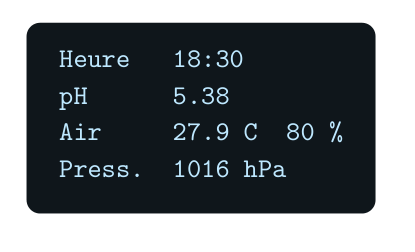
\includegraphics[width=0.3\textwidth]{img/inf/f_oled.png}
\caption{Contenu de l'écran avec le montage du 1\textsuperscript{er} novembre : heure 18:30, pH 5,38, air \qty{27,9}{\celsius} et \qty{80}{\percent}, pression \qty{1016}{hPa}.}
\end{figure}

% ---------------------------------------------------------------------
\Needspace{8\baselineskip}\subsection{Premières mesures réelles}

Une fois le matériel en service, j'enregistre les mesures pendant près d'une demi-heure, le 1er novembre de 18 h 20 à 18 h 48, avec les capteurs disponibles. Pendant cet essai, j'étalonne la sonde pH avec les solutions tampon pH 7 et pH 4, grâce aux boutons du dashboard. J'exporte les données depuis le dashboard (onglet Journal) et je les analyse ici. Cette sous-partie résume d'abord les mesures recueillies, puis compare le pH avant et après étalonnage. Elle montre ensuite ce que les valeurs du pH révèlent sur la précision de la mesure, et se termine par les anomalies repérées dans les données.

\subsubsection*{Les données recueillies}

143 mesures sont enregistrées, une toutes les \qty{11,6}{s} en moyenne (de \qty{11}{s} à \qty{14}{s}) : aux \qty{10}{s} d'attente prévues s'ajoute le temps de lecture des capteurs, surtout la sonde de l'eau, que le programme interroge même absente.

Le tableau suivant donne les mesures du 1\textsuperscript{er} novembre.

\begin{table}[H]
\centering
\small
\begin{tabularx}{\textwidth}{|l|l|c|c|c|c|}
\hline
\textbf{Grandeur} & \textbf{Capteur} & \textbf{Mesures} & \textbf{Minimum} & \textbf{Moyenne} & \textbf{Maximum} \\
\hline
pH (après étalonnage) & sonde pH sur A1 & 119 & 5,26 & 5,40 & 5,49 \\
\hline
Température de l'air & DHT20\ix{24} & 143 & \qty{27,8}{\celsius} & \qty{28,0}{\celsius} & \qty{28,1}{\celsius} \\
\hline
Humidité de l'air & DHT20\ix{24} & 143 & \qty{80}{\percent} & \qty{80}{\percent} & \qty{81}{\percent} \\
\hline
Pression de l'air & BMP280 & 143 & \qty{1016}{hPa} & \qty{1016}{hPa} & \qty{1016}{hPa} \\
\hline
\end{tabularx}
\caption{Mesures du 1er novembre.}
\end{table}

Pour le pH, la ligne du tableau ne garde que les mesures faites après l'étalonnage, hors un point isolé (voir la sous-partie suivante). L'air reste très stable pendant l'essai, ce qui est normal en intérieur sur une demi-heure : \qty{0,3}{\celsius} et \qty{1}{\percent} d'humidité d'écart. La pression, affichée au hPa près, ne bouge pas. EC, niveau, température de l'eau et batterie n'ont pas de valeur, leurs capteurs n'étant pas branchés ; la lumière, entre \qty{0}{\percent} et \qty{1}{\percent}, n'est que le bruit d'une entrée sans capteur.

\subsubsection*{Le pH avant et après étalonnage}

La courbe se lit en trois temps. Avant étalonnage (18 h 20 à 18 h 22), le programme utilise les valeurs par défaut du fabricant et affiche environ 4,5 : cette valeur n'a pas de sens physique tant que la sonde n'est pas étalonnée. Ensuite, dans la solution tampon pH 7 (18 h 24), la mesure monte à 6,88 -- 7,00 ; l'appui sur le bouton « pH 7,00 » enregistre la tension du moment comme référence. Enfin, après étalonnage (à partir de 18 h 25), le pH se stabilise à $5{,}40 \pm 0{,}04$ (moyenne $\pm$ écart-type, 119 mesures) dans l'eau mesurée.

La figure suivante montre le pH mesuré le 1\textsuperscript{er} novembre, avant et après étalonnage.

\begin{figure}[H]
\centering
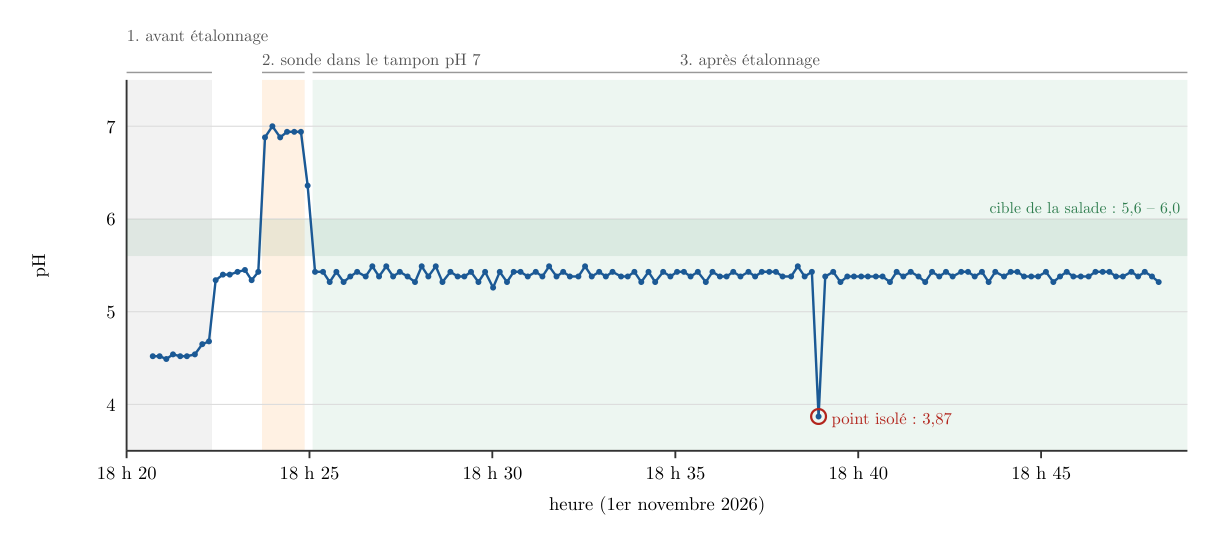
\includegraphics[width=\textwidth]{img/inf/f_ph_courbe.png}
\caption{pH mesuré le 1er novembre : avant étalonnage, dans la solution tampon pH 7, puis après étalonnage. La bande verte est la cible de la salade cultivée.}
\end{figure}

Cette valeur est en dessous de la cible de la salade (5,6 à 6,0). Le comportement attendu du pilote est alors de ne pas verser de pH$-$, qui ferait encore baisser le pH, et d'afficher l'avertissement « pH trop bas : pas de pH+, corriger à la main ». La mesure de 18 h 38 à 3,87 est un point isolé : la suivante revient aussitôt à 5,38. Elle correspond sans doute à une perturbation passagère (sonde bougée, bulle, faux contact). Une seule mesure de ce type ne déclenche pas de dose, puisque le pilote attend 10 minutes entre deux doses, mais un filtre qui écarte les valeurs isolées serait une amélioration utile.

\subsubsection*{La précision de la mesure du pH}

En regardant les valeurs une par une, je remarque que le pH ne prend que quelques valeurs bien précises : 5,26, 5,32, 5,38, 5,43 et 5,49. Ces « marches » sont la trace du convertisseur 10 bits de l'Arduino, qui ne distingue pas deux tensions séparées de moins de \qty{4,9}{mV}.

Le tableau suivant donne les valeurs de pH prises par la mesure après étalonnage.

\begin{table}[H]
\centering
\small
\begin{tabular}{|l|c|c|c|c|c|}
\hline
\textbf{pH affiché} & 5,26 & 5,32 & 5,38 & 5,43 & 5,49 \\
\hline
\textbf{Nombre de mesures} & 1 & 15 & 50 & 46 & 7 \\
\hline
\end{tabular}
\caption{Valeurs de pH prises par la mesure après étalonnage.}
\end{table}

\naturecalc{mesures du 1\textsuperscript{er} novembre sur le vrai matériel, comparées à la théorie}
\begin{demonstration}[ce que vaut une marche]
\resultat{\left|\Delta\mathrm{pH}\right| \approx 0{,}0275 \text{ par pas du convertisseur}}
D'après la droite d'étalonnage de la partie 8.4, le pH vaut $\mathrm{pH} = 7 + (U - U_7)\times\dfrac{4-7}{U_4 - U_7}$. Si la tension varie de $\Delta U$ (en mV), le pH varie de $\Delta\mathrm{pH}$ avec :
\begin{align*}
\mathrm{pH} + \Delta\mathrm{pH} &= 7 + (U + \Delta U - U_7)\times\frac{-3}{U_4 - U_7}\\
\Delta\mathrm{pH} &= \Delta U\times\frac{-3}{U_4 - U_7}
\end{align*}
En valeur absolue, la marche du pH vaut donc :
\[
\left|\Delta\mathrm{pH}\right| = \Delta U\times\frac{3}{U_4 - U_7}
\]
Une marche du convertisseur de l'Arduino correspond à un pas de $\Delta U = \dfrac{\qty{5000}{mV}}{1024} \approx \qty{4,88}{mV}$. L'étalonnage de la partie 8.4 donne $U_4 - U_7 = \qty{532}{mV}$, soit $\qty{532}{mV}/3 \approx \qty{177}{mV}$ par unité de pH. Pour un pas :
\begin{align*}
\left|\Delta\mathrm{pH}\right| &= \qty{4,88}{mV}\times\frac{3}{\qty{532}{mV}}\\
\left|\Delta\mathrm{pH}\right| &\approx 0{,}0275
\end{align*}
Les marches observées dans le relevé valent en moyenne, entre les valeurs extrêmes de 5,26 et de 5,49 séparées par 4 marches :
\begin{align*}
\Delta\mathrm{pH} &= \frac{5{,}49 - 5{,}26}{4}\\
\Delta\mathrm{pH} &= \frac{0{,}23}{4} = 0{,}0575
\end{align*}
Cela fait environ deux pas du convertisseur ($0{,}0575/0{,}0275 \approx 2{,}1$) : le bruit de la mesure saute souvent de deux pas à la fois. Avec l'ADS1115\ix{16} (pas de $\qty{0,1875}{mV}$ dans la plage par défaut), un pas ne vaudrait plus que :
\begin{align*}
\left|\Delta\mathrm{pH}\right| &= \qty{0,1875}{mV}\times\frac{3}{\qty{532}{mV}}\\
\left|\Delta\mathrm{pH}\right| &\approx 0{,}0011
\end{align*}
soit environ 26 fois moins que $0{,}0275$.
\end{demonstration}

Avec l'Arduino seul, le pH n'est donc connu qu'à environ \num{0,06} près (deux pas de bruit, soit \num{0,0575}). C'est suffisant pour surveiller, mais un peu juste pour doser au plus près d'une cible large de \num{0,4} seulement. Ces mesures confirment, avec des chiffres réels, le choix de l'ADS1115\ix{16} fait dans la partie 8.2.

\subsubsection*{Les anomalies des données}

L'export des journées du 31 octobre et du 1er novembre contient aussi des valeurs que j'écarte de l'analyse, parce qu'elles témoignent de défauts plutôt que de la réalité :

\begin{itemize}
\item \textbf{pH négatif le 31 octobre} (101 mesures, de $-5{,}91$ à $-0{,}20$) : enregistré avec l'ancien montage et sans étalonnage, il est physiquement impossible. Il montre qu'une mesure non étalonnée ou mal raccordée peut être totalement fausse, et pourquoi le pilote doit limiter le nombre de doses par jour.
\item \textbf{Température de l'eau à \qty{0,0}{\celsius}} le 1er novembre, sans aucune sonde branchée : c'est le deuxième défaut de la mise en service, corrigé depuis.
\item \textbf{Six lignes à l'heure incohérente} (de 19 h à 23 h le 1er novembre, alors que l'essai se déroule vers 18 h 30) : elles viennent probablement de la remise à l'heure au démarrage du serveur (horloge à pile ou Internet). Je les écarte ; ce point reste à vérifier.
\end{itemize}

\begin{aretenir}
Toute la chaîne de mesure fonctionne sur le vrai matériel : de la sonde au dashboard, en passant par l'Arduino, le Raspberry et la base de données. La sonde pH étalonnée donne une mesure stable ($\pm\num{0,04}$) ; sa finesse est limitée par le convertisseur de l'Arduino, ce que l'ADS1115\ix{16} corrigera.
\end{aretenir}


% ---------------------------------------------------------------------
\Needspace{8\baselineskip}\subsection{Essais}

Le matériel n'est pas encore disponible pendant l'écriture du programme. J'organise donc les essais en deux temps : d'abord tout vérifier sur ordinateur, ensuite préparer un essai complet à faire dès que la tour sera câblée. Je veux que cet essai se fasse d'un coup et qu'il indique, pour chaque échec, la piste à vérifier. Depuis le 1er novembre, une partie du matériel est en service (parties 8.7 et 8.8). Cette sous-partie présente les essais réalisés sans matériel et le défaut qu'ils révèlent, puis la procédure d'essai sur la tour. Elle fait enfin le point sur ce qui est déjà vérifié sur la tour et ce qui reste à confirmer.

\subsubsection*{Essais réalisés sans matériel}

Pour tester sans matériel, je simule l'Arduino. Une simulation trop simple ne prouverait rien : j'écris donc un faux Arduino qui répond aux vrais messages Firmata, pour que le code de communication soit réellement exercé, octet par octet. Voici ce que je vérifie sur ordinateur :

\begin{itemize}
\item \textbf{Conversions} : pH 7,00 à \qty{1500}{mV} et 4,00 à \qty{2032}{mV} ; \qty{1413}{\micro S/cm} pour la solution d'étalonnage ; niveau \qty{50}{\percent} à mi-course.
\item \textbf{Décisions} : scénario complet du pilote (doses espacées de \qty{10}{min}, coupure à \qty{29}{\percent}, reprise au soleil après 5 min, nouvel arrêt sans soleil, reprise à \qty{36}{\percent}, conseils sous \qty{30}{\percent} et \qty{35}{\percent}, stock bas).
\item \textbf{Dialogue avec l'Arduino} : un faux Arduino répond aux vrais messages Firmata (I2C\ix{12}, OneWire) ; il permet de vérifier la lecture de chaque capteur et l'ordre d'allumage des sondes.
\item \textbf{Dashboard} : réglages, conseils, doses manuelles, journal et alertes, testés dans un navigateur avec le serveur et l'Arduino simulé.
\end{itemize}

Ces essais font apparaître un défaut, corrigé depuis : quand l'EC reste trop basse, le pH n'est jamais corrigé ; les doses alternent maintenant entre engrais et pH$-$.

\subsubsection*{Procédure d'essai sur la tour}

Je choisis de tester tout le matériel d'un coup plutôt qu'élément par élément : le script donne un résultat pour chaque élément, ce qui permet de tout câbler puis de repérer aussitôt ce qui ne répond pas. Les essais des pompes demandent une confirmation, car seul l'opérateur peut voir si une pompe tourne vraiment.

Le script \texttt{essai\_materiel.py} teste tout le matériel d'un coup, avant de lancer le pilotage. Il affiche pour chaque élément OK ou ÉCHEC, avec un conseil de réparation. Il commence par les modules I2C\ix{12} : chaque module répond-il à son adresse ? Il passe ensuite aux capteurs, dont les valeurs sont à comparer avec la réalité (thermomètre, main sur le capteur de lumière\ldots). Il teste alors l'alternance pH / EC, en mesurant le pH sonde EC éteinte puis allumée. Il vérifie l'écran OLED, qui doit afficher « ESSAI HYDROTOUR », puis les pompes : chacune tourne de \qty{2}{s} à \qty{5}{s} et l'opérateur confirme. Il termine par la sécurité : le Raspberry se tait volontairement, et la pompe doit s'arrêter seule après \qty{30}{s}.

Le guide \texttt{ESSAIS.md} détaille ensuite l'étalonnage et les vérifications du pilotage (cycle court, coupure de la batterie forcée, mode manuel).

\subsubsection*{Ce qui est vérifié et ce qui reste à vérifier}

Je préfère lister honnêtement ce qui n'a pas encore été vérifié. Certains points ne peuvent être confirmés qu'avec le vrai matériel, comme le temps de retour de la sonde pH ou le débit réel des doseuses.

\textbf{Vérifié sur la tour (1er novembre) :}

\begin{itemize}
\item la compilation et le téléversement de \texttt{HydroTour\_Firmata}, et le dialogue Firmata avec le Raspberry ;
\item la lecture du DHT20\ix{24}, du BMP280 et de l'horloge, et l'affichage de l'écran ;
\item la lecture et l'étalonnage de la sonde pH (branchée provisoirement sur A1) ;
\item l'enregistrement des mesures, le dashboard et l'export des données ;
\item l'accès depuis Internet, la page de connexion et le refus de \texttt{/api/data} par Internet.
\end{itemize}

\textbf{Points à confirmer sur le vrai matériel :}

\begin{itemize}
\item l'ADS1115\ix{16}, puis la sonde pH sur celui-ci, la sonde EC et le ruban de niveau ;
\item la carte 8 MOSFET\ix{15}, les pompes et la sécurité des \qty{30}{s} ;
\item la lecture de la DS18B20\ix{24} ;
\item le sens du courant de l'INA260\ix{22} (charge positive au soleil) ;
\item le temps de retour du pH après la lecture de l'EC (\qty{5}{s} prévues) ;
\item le débit réel des doseuses, pour ajuster la durée des doses ;
\item l'étalonnage du ruban, et la cause des lignes à l'heure incohérente (partie 8.8) ;
\item l'essai complet avec \texttt{essai\_materiel.py}, une fois tout câblé.
\end{itemize}

% ---------------------------------------------------------------------
\Needspace{8\baselineskip}\subsection{Synthèse de l'étude informatique}

Pour faire le point, je reprends chaque fonction de la tour avec la solution retenue et son état d'avancement. Je tiens à distinguer ce qui est vérifié sur la tour, ce qui est écrit et testé sur ordinateur, et ce qui reste à essayer : cela montre exactement où en est le projet et par où continuer. Cette sous-partie rassemble dans un tableau les fonctions de la tour, les solutions retenues et leur état, puis dresse le bilan du programme.

\begin{table}[H]
\centering
\small
\begin{tabularx}{\textwidth}{|l|Y|l|}
\hline
\textbf{Fonction} & \textbf{Solution retenue} & \textbf{État} \\
\hline
Répartition des rôles & Raspberry : décisions en Python ; Arduino : ConfigurableFirmata & vérifié sur la tour \\
\hline
Mesures de l'air et heure & DHT20\ix{24}, BMP280 et horloge sur le bus I2C\ix{12} & vérifié sur la tour \\
\hline
Mesure du pH & ADS1115\ix{16} 16 bits ; en attendant, entrée A1 de l'Arduino (10 bits) & provisoire \\
\hline
Étalonnage & boutons pH 7, pH 4, vide, plein dans le dashboard & pH fait \\
\hline
Supervision & dashboard web, alertes, journal, écran OLED & vérifié sur la tour \\
\hline
Accès à distance & Tailscale\ix{20} Funnel\ix{20} ; identifiant, mot de passe et captcha & en service \\
\hline
Sécurité de liaison & coupure des pompes après \qty{30}{s} sans message & à essayer \\
\hline
Commande des pompes & carte 8 MOSFET\ix{15} I2C\ix{12}, sorties 0 à 3 & à essayer \\
\hline
Mesures EC et niveau & EC : sonde fabriquée sur D5, D6 et A0 ; niveau : ADS1115\ix{16} 16 bits & à essayer \\
\hline
Perturbation pH / EC & sonde pH coupée par la sortie 4, sonde EC alimentée par D5 et D6 & à essayer \\
\hline
Arrosage & cycle réglable, arrêt si réservoir sous \qty{15}{\percent} & écrit, testé \\
\hline
Protection de la batterie & coupure \qty{30}{\percent}, reprise \qty{35}{\percent} ou au soleil (\qty{1,5}{A} et \qty{60}{\percent}) & écrit, testé \\
\hline
Dosage & cibles selon légume et stade, doses de \qty{3}{s} / \qty{2}{s}, \qty{10}{min} d'écart, 12 par jour & écrit, testé \\
\hline
\end{tabularx}
\caption{Fonctions de la tour, solutions retenues et état.}
\end{table}

« Vérifié sur la tour » signifie essayé avec le vrai matériel le 1er novembre ; « écrit, testé » signifie vérifié sur ordinateur avec un Arduino simulé. Les essais suivants, guidés par \texttt{essai\_materiel.py}, valideront le reste au fur et à mesure du câblage.

Le programme est prêt à piloter la tour seule : il arrose, nourrit les plantes selon leur stade, protège sa batterie et prévient quand il a besoin d'une intervention. Les réglages se font depuis le dashboard, sans toucher au code, et chaque décision est expliquée dans le journal. Depuis novembre, la tour se surveille aussi depuis n'importe où, derrière une page de connexion, et les premières mesures réelles confirment que la chaîne complète fonctionne, de la sonde jusqu'au téléphone.

% ---------------------------------------------------------------------
\Needspace{8\baselineskip}\subsection{Organisation des fichiers}

Pour qu'une autre personne puisse reprendre le projet, je rassemble chaque fichier avec son rôle. Je fais en sorte que le dossier \texttt{SERVEUR} se suffise à lui-même : il suffit de le copier sur le Raspberry pour que tout fonctionne. Cette sous-partie donne la liste des fichiers du projet avec le rôle de chacun, puis les commandes pour installer et lancer la tour. Tous ces fichiers sont depuis le 20 novembre 2026 sur le dépôt GitHub du projet, dont la partie 9.6 donne l'adresse et le contenu.

\begin{table}[H]
\centering
\small
\begin{tabularx}{\textwidth}{|l|Y|}
\hline
\textbf{Fichier} & \textbf{Rôle} \\
\hline
\texttt{ARDUINO/HydroTour\_Firmata} & programme de l'Arduino : ConfigurableFirmata et sécurité de \qty{30}{s} \\
\hline
\texttt{SERVEUR/server.py} & programme principal : boucle de mesure, base de données, dashboard, écran \\
\hline
\texttt{SERVEUR/pilote.py} & décisions : cycle, batterie, soleil, dosage, alertes ; conversions \\
\hline
\texttt{SERVEUR/arduino.py} & dialogue avec l'Arduino et lecture de chaque capteur \\
\hline
\texttt{SERVEUR/hydrotour.html} & dashboard ; contient aussi le tableau des légumes \\
\hline
\texttt{SERVEUR/essai\_materiel.py} & essai de tout le matériel \\
\hline
\texttt{SERVEUR/ESSAIS.md} & guide des essais et de l'étalonnage \\
\hline
\texttt{SERVEUR/fausses\_mesures.py} & fausses mesures pour essayer le dashboard sans capteurs \\
\hline
\texttt{SERVEUR/acces.py} & page de connexion, captcha, identifiant et mot de passe partagés \\
\hline
\texttt{SERVEUR/diagnostic.py} & liste les modules et capteurs qui répondent vraiment \\
\hline
\texttt{SERVEUR/INTERNET.md} & guide de l'accès par Internet (Tailscale\ix{20} Funnel\ix{20}) et du premier accès \\
\hline
\texttt{ARDUINO/HydroTour\_Firmata\_uno.hex} & programme de l'Arduino déjà compilé pour l'Uno, à téléverser avec \texttt{avrdude} \\
\hline
\end{tabularx}
\caption{Fichiers du projet.}
\end{table}

Pour installer la tour, il suffit de copier le dossier \texttt{SERVEUR} sur le Raspberry (dans \texttt{\textasciitilde/hydrotour}) et d'exécuter :

\begin{verbatim}
sudo apt install python3-flask python3-pil
python3 -m venv --system-site-packages venv
venv/bin/pip install pyfirmata2
venv/bin/python -u server.py
\end{verbatim}

Sur la tour, la dernière commande est lancée par le service \texttt{hydrotour.service} à chaque démarrage. Pour l'accès par Internet, il faut en plus publier le port 5001 avec \texttt{sudo tailscale funnel --bg 5001} (guide \texttt{INTERNET.md}).

% ---------------------------------------------------------------------
\Needspace{8\baselineskip}\subsection{La première version du programme : cerveau.py}

Avant l'étude précédente, j'avais écrit une première architecture, dans laquelle un seul programme du Raspberry (\texttt{cerveau.py}) dialoguait avec un Arduino à lignes de texte. Je la garde ici parce que le code correspondant existe encore dans le dossier du projet et que d'autres parties du rapport s'y réfèrent, par exemple la détection de chute (partie 4). Les sous-parties précédentes décrivent la version actuelle ; celles-ci décrivent la première. Seule la version actuelle (\texttt{server.py}, \texttt{pilote.py} et \texttt{arduino.py}) est à installer sur le Raspberry (tutoriel de la partie 10) ; la première version est conservée pour mémoire, et c'est elle qui avait la sécurité de niveau dans l'Arduino.


\subsubsection*{Le choix d'architecture : un cerveau et un exécutant}

Je cherche un système qui lise les capteurs, décide, commande les pompes et se laisse surveiller à distance. Le Raspberry Pi 3 B est un vrai petit ordinateur : il garde l'historique, fait tourner un serveur web et peut être programmé en Python. Mais il n'a pas d'entrées analogiques et il peut se bloquer. L'Arduino Uno R3 n'a presque aucune mémoire, mais il lit les capteurs de façon fiable et fait ce qu'on lui demande, sans jamais s'arrêter. Je répartis donc les rôles ainsi :

\textbf{Le Raspberry Pi est le cerveau.} Il tourne sous Python (programme \texttt{cerveau.py}), garde les mesures dans une base de données, décide quand doser et quand faire circuler l'eau, et sert le dashboard.

\textbf{L'Arduino est l'exécutant et le garde-fou.} Il lit les capteurs en valeurs brutes, commande les pompes sur ordre du Pi, et applique seul les sécurités. Toute la logique est sur le Pi, toute la protection est sur l'Arduino : si le Pi plante, la tour ne peut pas se noyer ni se vider.

Les deux cartes communiquent par le câble USB, à \qty{115200}{bauds}, par des lignes de texte. Le Pi envoie des ordres courts et l'Arduino répond.

\begin{table}[H]
\centering
\small
\begin{tabularx}{\textwidth}{|c|Y|Y|}
\hline
\textbf{Ordre du Pi} & \textbf{Ce qu'il demande} & \textbf{Réponse de l'Arduino} \\
\hline
\texttt{P} & Es-tu là ? & \texttt{OK P} \\
\hline
\texttt{L} & Lis tous les capteurs & une ligne \texttt{M} avec pH, EC, niveau, température de l'eau et de l'air, humidité, lumière, inclinaison \\
\hline
\texttt{D <c> <ms>} & Fais tourner la pompe $c$ pendant $ms$ millisecondes (0 : circulation, 1 : engrais A, 2 : engrais B, 3 : pH$-$) & \texttt{OK D ...} ou \texttt{ERR ...} \\
\hline
\texttt{S} & Arrête toutes les pompes & \texttt{OK S} \\
\hline
\texttt{E} & Donne ton état & état des pompes, du mode secours, de la chute, du niveau \\
\hline
\texttt{N}, \texttt{Z}, \texttt{R} & Règle le seuil de niveau, mémorise la tour droite, réarme après une chute & \texttt{OK ...} \\
\hline
\end{tabularx}
\caption{Les ordres échangés entre le Raspberry Pi et l'Arduino.}
\end{table}

\subsubsection*{Les sécurités de l'Arduino}

Chaque durée de pompe est limitée : \qty{30}{s} au maximum pour une doseuse (\qty{30000}{ms}) et \qty{1000}{s} pour la circulation. Un ordre trop long reçoit la réponse \texttt{ERR duree}. L'Arduino applique ensuite quatre protections.

\textbf{Le niveau bas.} Si le niveau d'eau passe sous le seuil réglé, la circulation est coupée (une pompe qui tourne à sec s'abîme), mais les doseuses restent permises. Elle reprend quand le niveau remonte de plus de \qty{50}{mV} au-dessus du seuil (hystérésis\ix{31}, pour éviter de couper et reprendre sans cesse).

\textbf{La chute.} Si la tour penche de plus de \ang{35} pendant plus d'une seconde (calcul de la partie 7), toutes les pompes s'arrêtent et refusent tout ordre, jusqu'à ce que la tour soit redressée et réarmée.

\textbf{Le chien de garde.} Si le programme de l'Arduino se bloque pendant plus de \qty{8}{s}, il redémarre seul, et toutes les pompes repartent à l'arrêt.

\textbf{Le mode secours.} Si le Pi n'envoie plus rien pendant 5 minutes, l'Arduino passe en mode secours : la circulation tourne \qty{15}{min} puis s'arrête \qty{15}{min}, sans aucun dosage. Dès qu'un ordre arrive, le mode secours s'arrête. Ainsi, une panne du Pi ne tue pas les plantes : l'eau continue de circuler.

\subsubsection*{Le pilotage : planning, cibles et dosage}

Le Pi suit un planning de circulation : de 6 h à 18 h, \qty{15}{min} de marche puis \qty{15}{min} d'arrêt ; la nuit, \qty{15}{min} à 21 h, 0 h et 3 h. L'Arduino limite une commande à environ \qty{1000}{s} : pour une marche de \qty{15}{min}, le Pi envoie un ordre de \qty{90}{s} qu'il renouvelle toutes les minutes environ (un « bail »). Si le Pi se tait, la pompe s'arrête d'elle-même au bout de \qty{90}{s}.

Les cibles viennent de la recherche documentaire sur les besoins des plantes. Pour la laitue en croissance des feuilles, le pH visé est de 5,6 à 6,0 et l'EC de \qtyrange{1,2}{1,6}{mS/cm} (\qtyrange{1200}{1600}{\micro S/cm}) ; le dosage vise le milieu de la plage, soit environ \qty{1,4}{mS/cm}. L'alarme de température de l'eau se déclenche au-dessus de \qty{28}{\celsius}. Le dashboard contient le tableau des légumes (laitue, tomate cerise, poivron) avec leurs plages par stade de croissance.

\naturecalc{théorie (hypothèses à mesurer : sensibilité de l'EC et débit des doseuses)}
\begin{demonstration}[volume d'engrais pour remonter l'EC]
\resultat{V_A = \dfrac{(EC_{cible} - EC_{mes})\; V_{bac}}{s}}
Je note $EC_{mes}$ l'EC mesurée, en mS/cm, $EC_{cible}$ la cible, en mS/cm, $V_{bac}$ le volume du bac, en litres (\qty{152}{L}), $V_A$ le volume de solution mère A à ajouter, en mL (le même volume de B est ajouté), et $s$ l'augmentation d'EC provoquée par \qty{1}{mL} de A et \qty{1}{mL} de B par litre de bac, en (mS/cm)/(mL/L). Je prends $s = \qty{0,56}{(mS/cm)/(mL/L)}$ (hypothèse à mesurer). En solution diluée, l'EC est proportionnelle à la quantité de sels. Elle augmente donc proportionnellement à la dose $d$ (en mL par litre de bac) :
\begin{align*}
\Delta EC &= s\,d
\end{align*}
La dose est le volume ajouté divisé par le volume du bac, $d = V_A/V_{bac}$. En remplaçant et en isolant $V_A$ :
\begin{align*}
\Delta EC &= s\,\frac{V_A}{V_{bac}}\\
V_A &= \frac{\Delta EC\; V_{bac}}{s}
\end{align*}
Avec $\Delta EC = EC_{cible} - EC_{mes}$. Application : EC mesurée \qty{1,20}{mS/cm}, cible \qty{1,40}{mS/cm} :
\begin{align*}
V_A &= \frac{(\qty{1,40}{mS/cm} - \qty{1,20}{mS/cm}) \times \qty{152}{L}}{\qty{0,56}{(mS/cm)/(mL/L)}}\\
V_A &= \frac{\qty{30,4}{mS/cm\cdot L}}{\qty{0,56}{(mS/cm)/(mL/L)}}\\
V_A &\approx \qty{54,3}{mL}
\end{align*}
La durée de marche d'une pompe de débit $Q$ est le volume divisé par le débit, $t = V/Q$. Avec $Q = \qty{80}{mL/min}$ (hypothèse à mesurer, mesure M5) :
\begin{align*}
t &= \frac{\qty{54,3}{mL}}{\qty{80}{mL/min}} \approx \qty{0,679}{min} \approx \qty{40,7}{s}
\end{align*}
Cette durée dépasse la limite de \qty{30}{s} : le Pi découpe la dose en deux ordres d'environ \qty{20,4}{s}, espacés pour laisser l'eau se mélanger, et il mesure de nouveau l'EC avant de continuer.
\end{demonstration}

\subsubsection*{Le serveur et le dashboard}

Le Pi héberge un serveur web écrit en Python avec Flask (programme \texttt{server.py}, port 5000), protégé par un identifiant et un mot de passe. Il enregistre toutes les mesures dans une base SQLite, avec l'heure en temps universel, et répond à des adresses web simples : les dernières mesures, l'historique, le journal des actions et un export des données au format CSV. La page du dashboard (\texttt{hydrotour.html}) se met à jour toutes les 10 secondes. Pour y accéder depuis l'extérieur sans toucher à la box Internet, je passe par Tailscale\ix{20} ; Raspberry Pi Connect permet en plus de prendre la main sur le Pi. Les captures ci-dessous viennent du dashboard branché sur un Arduino simulé.

\begin{figure}[H]
\centering
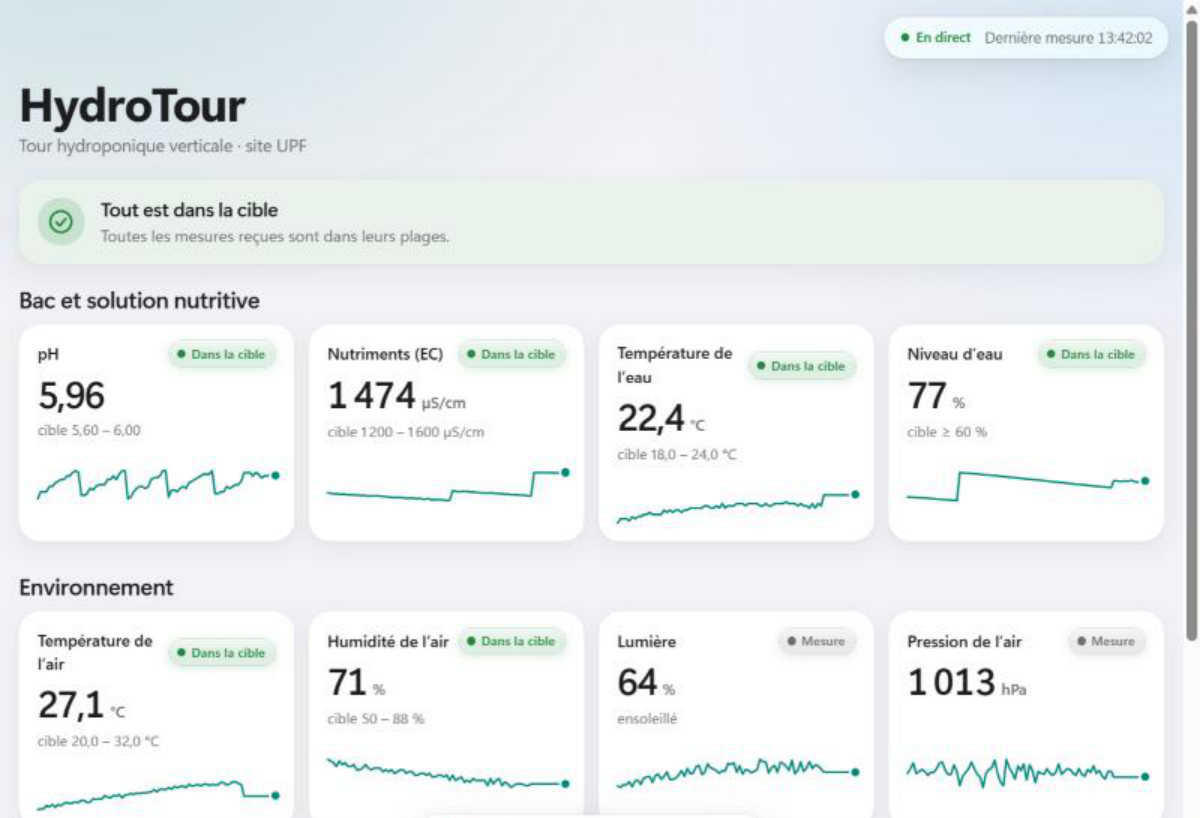
\includegraphics[width=0.82\textwidth]{img/dash_mesures.png}
\caption{Onglet Mesures : chaque tuile indique la valeur, la cible du légume et la courbe des dernières heures ; le bandeau du haut résume l'état.}
\end{figure}

\begin{figure}[H]
\centering
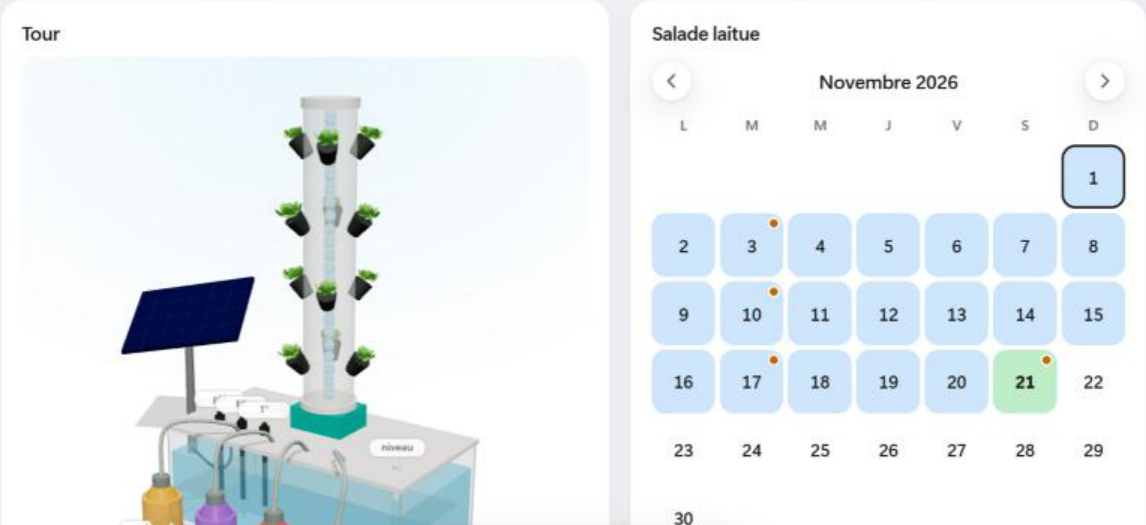
\includegraphics[width=0.82\textwidth]{img/dash_tour.png}
\caption{Onglet Installation : la tour en 3D suit le stade de la plante et le calendrier rappelle les contrôles.}
\end{figure}

\begin{figure}[H]
\centering
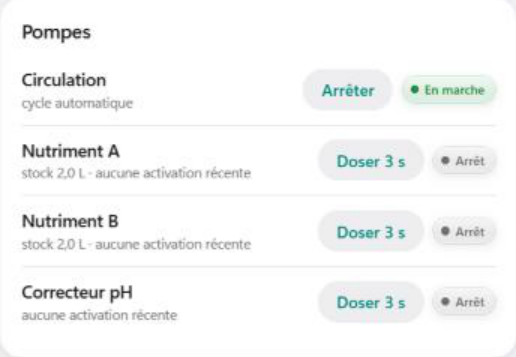
\includegraphics[width=0.55\textwidth]{img/dash_pompes.png}
\caption{Carte des pompes : état de chacune, dose manuelle de \qty{3}{s} et stock d'engrais restant.}
\end{figure}

\begin{figure}[H]
\centering
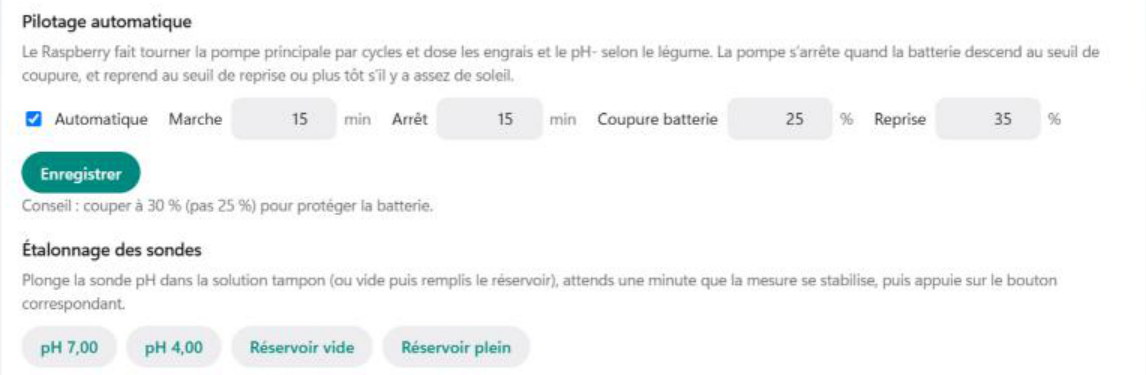
\includegraphics[width=0.9\textwidth]{img/dash_param.png}
\caption{Réglages du pilotage automatique et étalonnage des sondes (pH 7, pH 4, réservoir vide, réservoir plein).}
\end{figure}

Pour se rendre compte du fonctionnement réel du site, j'ai publié une copie de démonstration du dashboard, identique à l'interface réelle mais alimentée par des mesures fictives et figées : \href{https://claude.ai/artifact/G8rZH2kN7ZYfnY5RFY4Tiu}{\textbf{ouvrir le dashboard de démonstration}} (adresse complète : \url{https://claude.ai/artifact/G8rZH2kN7ZYfnY5RFY4Tiu}). La page s'ouvre sur l'écran de connexion. L'identifiant est \texttt{demo} et le mot de passe est \texttt{hydrotour-demo}. Il faut aussi recopier les cinq caractères du captcha affiché (le bouton « Autre image » en génère un nouveau). Les quatre onglets se parcourent comme sur la tour. Les ordres envoyés aux pompes n'agissent sur aucun matériel, et l'export du journal ne fonctionne pas dans cette version.

Un appui manuel sur la circulation met l'automatique en pause : sans cela, le Pi rallumerait la pompe dix secondes plus tard. Le serveur refuse les réglages absurdes, par exemple une reprise trop proche du seuil de coupure de la batterie.

\subsubsection*{Ce qui est fait et ce qui ne l'est pas}

\textbf{Vérifié sur le vrai matériel :} la sonde de pH étalonnée dans des solutions de référence, la chaîne de la sonde jusqu'au téléphone, le dashboard avec un Arduino simulé. \textbf{Compilé mais pas essayé sur la carte :} le programme de l'Arduino (flash \qty{23216}{octets} sur \qty{32256}{octets}, soit 72\,\% ; mémoire vive \qty{681}{octets} sur \qty{2048}{octets}, soit 33\,\%). \textbf{Compilé mais pas encore relu en entier :} \texttt{cerveau.py} (environ 1400 lignes). \textbf{Reste à faire :} un faux Arduino pour tester sans matériel, la relecture de \texttt{cerveau.py}, le script d'étalonnage, le fichier de configuration et le démarrage automatique du programme au branchement.

\begin{aretenir}
Le Raspberry Pi décide, l'Arduino exécute et protège : niveau bas, chute au-delà de \ang{35}, chien de garde de \qty{8}{s} et mode secours de la circulation après 5 minutes de silence. Une dose d'engrais se calcule par $V_A = \Delta EC\,V_{bac}/s$ (\qty{54}{mL} pour passer de \qty{1,20}{mS/cm} à \qty{1,40}{mS/cm}, hypothèses à mesurer). Le dashboard permet de tout surveiller et régler depuis un téléphone. Le programme de l'Arduino n'a pas encore tourné sur la carte.
\end{aretenir}


% =====================================================================
% PARTIE : LE DEPLOIEMENT DU 20 NOVEMBRE 2026
\clearpage
\partieENO{Le déploiement du 20 novembre 2026}

Cette partie est le compte rendu de la journée du 20 novembre 2026, au cours de laquelle la sonde de conductivité est passée de la conception à la mesure réelle. Je commence par la commande de mesure ajoutée au programme de l'Arduino, celle que la partie 7.6 annonçait comme restant à écrire. Je présente ensuite le calcul et l'étalonnage installés sur le Raspberry, puis la chaîne de compilation montée sur le Raspberry lui-même, qui permet de reprogrammer l'Arduino sans débrancher le câble. Je donne la première mesure obtenue dans l'eau. Je décris ensuite le nouvel écran d'étalonnage du dashboard. Je termine par le dépôt GitHub qui réunit tout le code, et par les problèmes rencontrés dans la journée avec la solution retenue pour chacun.

% ---------------------------------------------------------------------
\Needspace{8\baselineskip}\subsection{La commande de mesure dans l'Arduino}

La partie 7.6 explique pourquoi la mesure doit se faire entièrement dans l'Arduino : une phase dure environ \qty{130}{\micro s}, alors qu'un aller-retour par le câble USB dure plusieurs millisecondes. Cette commande est maintenant écrite et installée.

Elle s'ajoute au programme \texttt{HydroTour\_Firmata} sous la forme d'une fonctionnalité Firmata, c'est-à-dire d'un morceau de programme qui répond à un numéro de commande qui lui est propre. J'ai pris le numéro \texttt{0x0E}, qui fait partie des numéros laissés libres par la norme Firmata pour les commandes que chacun ajoute. Le Raspberry envoie trois octets, le début de message, le numéro de la commande, la fin de message. L'Arduino répond par les deux sommes $S_1$ et $S_2$, chacune découpée en trois paquets de sept bits, parce que Firmata ne transporte que des octets de sept bits.

À la réception, l'Arduino met D5 et D6 en sortie, fait soixante-quatre fois les deux phases, puis remet les deux broches en entrée pour déconnecter la sonde. Dans chaque phase, il attend \qty{20}{\micro s} que la tension se stabilise, lit l'entrée A0 et ajoute la lecture à la somme de cette phase. Les deux phases ont exactement la même durée, une attente et une conversion analogique, si bien que le courant moyen dans l'eau est nul, condition posée à la partie 7.4. La mesure complète dure environ \qty{17}{ms}, et la sonde reste déconnectée le reste du temps.

\Needspace{8\baselineskip}\subsection{Le calcul et l'étalonnage sur le Raspberry}

Le Raspberry reçoit les deux sommes et fait le reste, dans l'ordre démontré à la partie 7.7. Il calcule d'abord le rapport $x = S_1/S_2$, puis la résistance de l'eau $R_w = R_1 + P\,(x-1)$, puis la conductivité $\sigma_T = K/R_w$, qu'il ramène enfin à \qty{25}{\celsius} avec le coefficient $\alpha$. Ces calculs sont dans \texttt{pilote.py}, avec la démonstration de chaque formule en commentaire, et les valeurs de départ sont $R_1 = \qty{340}{\ohm}$, $P = \qty{365}{\ohm}$, $K = \qty{0,489}{cm^{-1}}$ et $\alpha = \qty{0,02}{\per\celsius}$.

La sonde EC perturbant la sonde pH, la carte de cette dernière est coupée pendant la mesure, par la sortie 4 de la carte 8 MOSFET\ix{15}, et le pH n'est pas lu dans les cinq secondes qui suivent. La mesure de l'EC a lieu une fois par minute, le pH toutes les dix secondes, conformément à la partie 7.6.

L'étalonnage à deux solutions est fait depuis le dashboard. Le Raspberry garde, pour chaque solution, sa conductivité et le rapport $x$ mesuré dedans, puis calcule $P$ et $K$ dès que les deux points sont connus. Si le résultat n'a pas de sens, c'est-à-dire si $P$ ou $K$ est négatif, il refuse l'étalonnage et demande de recommencer.

\Needspace{8\baselineskip}\subsection{Compiler et téléverser depuis le Raspberry}

Reprogrammer l'Arduino depuis l'ordinateur obligerait à débrancher le câble USB du Raspberry, à le brancher sur l'ordinateur, puis à le remettre. J'ai donc installé sur le Raspberry \texttt{arduino-cli}, qui est l'environnement Arduino sans fenêtres, avec le compilateur AVR et la bibliothèque \texttt{ConfigurableFirmata}. Le Raspberry compile désormais le programme et le téléverse lui-même, par le câble déjà en place.

\begin{verbatim}
curl -fsSL https://raw.githubusercontent.com/arduino/arduino-cli/master/install.sh \
  | BINDIR=~/outils sh
~/outils/arduino-cli core install arduino:avr
~/outils/arduino-cli lib install ConfigurableFirmata
\end{verbatim}

La compilation se fait sans arrêter la tour, puisqu'elle ne touche à rien. Le téléversement, lui, demande d'arrêter le service \texttt{hydrotour} le temps de l'opération, car ce service occupe le port USB en permanence. Les pompes se coupent alors d'elles-mêmes par la sécurité des trente secondes.

\begin{verbatim}
~/outils/arduino-cli compile --fqbn arduino:avr:uno HydroTour_Firmata
sudo systemctl stop hydrotour
~/outils/arduino-cli upload -p /dev/ttyACM0 --fqbn arduino:avr:uno HydroTour_Firmata
sudo systemctl start hydrotour
\end{verbatim}

Le programme occupe \qty{13110}{octets} de mémoire programme sur les \qty{32256}{} disponibles, soit \qty{40}{\percent}, et \qty{906}{octets} de mémoire vive sur \qty{2048}{}, soit \qty{44}{\percent}. L'ancien programme compilé, \texttt{HydroTour\_Firmata\_uno.hex}, est conservé : il suffit de le téléverser pour revenir en arrière.

\Needspace{8\baselineskip}\subsection{La première mesure}

Sonde en l'air, les deux sommes valent \num{65467} et \num{65470}, c'est-à-dire presque le maximum de \num{65472}. C'est le résultat attendu : sans eau entre les mines, le courant ne passe pas.

Sonde dans l'eau du réservoir, la chaîne complète a donné sa première valeur le 20 novembre 2026 à \qty{13}{h}\,\qty{21}{min}, heure de Tahiti :

\begin{verbatim}
2026-11-20T23:21:34Z {'ph': 7.67, 'ec': 1438, 'temp_air': 31.0,
                      'humidite': 70.9, 'lux': 2.0}
\end{verbatim}

Cette valeur de \qty{1438}{\micro S\per cm} est obtenue avec l'étalonnage de départ, et non avec un étalonnage mesuré : elle montre que la chaîne fonctionne de bout en bout, pas qu'elle est juste. La sonde DS18B20\ix{24} de l'eau n'étant pas encore branchée, le calcul suppose \qty{25}{\celsius} et n'applique donc aucune correction de température. L'étalonnage à deux solutions reste à faire, et c'est lui qui donnera la justesse annoncée à la partie 7.8.

\Needspace{8\baselineskip}\subsection{Le nouvel écran d'étalonnage}

L'écran d'étalonnage du dashboard ne proposait que quatre boutons, avec des valeurs figées : pH \num{7,00}, pH \num{4,00}, réservoir vide et réservoir plein. Je l'ai découpé en quatre sous-sections, une par sonde, et j'ai rendu les valeurs libres.

Pour le pH, les deux solutions tampons ne sont plus imposées. La conversion passe maintenant par la droite qui joint les deux points d'étalonnage, ce qui permet d'utiliser n'importe quel couple de tampons, par exemple \num{6,86} et \num{4,01}, ou \num{7,00} et \num{10,01} :

\[ \mathrm{pH} = \mathrm{pH}_1 + (U - U_1)\,\frac{\mathrm{pH}_2 - \mathrm{pH}_1}{U_2 - U_1} \]

Pour l'EC, la conductivité de chaque solution étalon se saisit en \unit{\micro S\per cm} au lieu d'être figée à \qty{1,413}{mS\per cm} et \qty{12,88}{mS\per cm}. Pour le niveau d'eau, les deux boutons sont conservés. Pour la température, une sous-partie nouvelle permet de saisir la température lue sur un thermomètre de référence : le programme enregistre l'écart avec la sonde et l'ajoute à toutes les mesures suivantes.

Chaque sous-section affiche en permanence la valeur brute lue par le capteur, la tension pour le pH, le rapport $x$ pour l'EC, la résistance pour le ruban, et l'étalonnage actuellement en mémoire. Chacune donne enfin son protocole en étapes numérotées, pour qu'il n'y ait pas à revenir au rapport pour étalonner.

L'étalonnage du pH déjà enregistré dans la base n'est pas perdu : au premier démarrage, le programme recopie les anciennes valeurs dans la nouvelle forme, une seule fois.

\Needspace{8\baselineskip}\subsection{Le dépôt GitHub}

Tout le code du projet est désormais sur GitHub, ce qui donne une sauvegarde hors du Raspberry et de mon ordinateur, et permet de suivre ce qui change d'une version à l'autre.

\textbf{Adresse :} \url{https://github.com/enoaarii/Projet-Hydroponique-}

Le dossier \texttt{HYDROCODE/} contient le code réellement installé sur la tour : le programme de l'Arduino et son binaire de secours, les quatre programmes Python du Raspberry, le dashboard, les outils de diagnostic et d'essai, et la copie de démonstration. Le dossier \texttt{archive\_premiere\_version/} contient la première architecture, celle du programme unique \texttt{cerveau.py} décrit à la partie 8.12 : elle est gardée pour mémoire et n'est pas installée. Les dossiers \texttt{etudes/}, \texttt{documents/} et \texttt{resume/} contiennent les sources des études, les PDF compilés et les résumés.

Les fichiers qui contiennent des secrets ou des données ne sont jamais envoyés : le fichier d'identifiants, la clé de session, la base de données et les fichiers d'étalonnage sont exclus par le fichier \texttt{.gitignore}. Le travail se fait sur une branche séparée, puis la branche est fusionnée dans la branche principale une fois relue.

Pour récupérer tout le code sur une machine neuve, une seule commande suffit.

\begin{verbatim}
git clone https://github.com/enoaarii/Projet-Hydroponique-.git
\end{verbatim}

\Needspace{8\baselineskip}\subsection{Les problèmes rencontrés et leurs solutions}

Quatre problèmes ont occupé la journée. Je les donne avec leur symptôme, leur cause et la correction retenue, parce que les trois derniers sont du genre à se reproduire.

\textbf{Le code du dépôt ne correspondait pas à celui de la tour.} J'avais d'abord écrit la sonde EC dans \texttt{cerveau.py}, le programme de la première architecture, avec un Arduino commandé par lignes de texte. Or la tour tourne avec \texttt{server.py}, \texttt{pilote.py}, \texttt{arduino.py} et Firmata. Téléverser le programme écrit pour la première architecture aurait fait perdre la mesure de la batterie, la pression, l'écran, l'horloge et la page de connexion. La relecture de la partie 8.12 de ce rapport a tranché : seule la version actuelle est installée. J'ai donc repris le travail sur le code réellement en service, et rangé la première version dans \texttt{archive\_premiere\_version/}.

\textbf{Deux versions différentes du même fichier.} Le fichier \texttt{arduino.py} du Raspberry faisait \qty{19118}{octets}, celui de mon ordinateur \qty{20052}{octets}. Le Raspberry tournait donc avec une version antérieure à mes améliorations de l'écran. J'ai comparé les empreintes des deux fichiers pour en être sûr, puis déployé la version récente, qui apporte l'écran en plus de la sonde. C'est le dépôt GitHub qui empêche désormais ce genre d'écart.

\textbf{La réponse de la mesure EC n'arrivait jamais.} Le programme du Raspberry demandait la mesure et n'obtenait rien, une seconde durant, puis abandonnait. En parlant à l'Arduino directement, sans passer par la bibliothèque, la réponse arrivait pourtant bien, en quelques millisecondes. La cause est dans la bibliothèque \texttt{pyfirmata2} : lorsqu'elle reçoit un message dont le numéro ne lui est pas connu, elle l'abandonne en plein milieu sans aller jusqu'à sa fin, puis lit la suite de ce message comme si c'étaient de nouvelles commandes. Le flux se décale, et la réponse suivante est perdue. Or les modules du bus I2C\ix{12} n'étant pas tous branchés, l'Arduino envoyait justement des messages de texte pour signaler ses erreurs de lecture. J'ai reproduit le défaut hors de la tour pour en être certain : sans gestionnaire de texte, la réponse disparaît ; avec, elle arrive. La correction tient en deux points, traiter les messages de texte, ce qui empêche le flux de se décaler, et réessayer une fois la mesure si la réponse manque malgré tout.

\textbf{Un essai qui ne prouvait rien.} Mon premier programme d'essai n'avait reçu aucune réponse, ce qui m'a fait croire un moment que l'Arduino était en cause. En réalité, il n'appelait pas la fonction qui lance le fil de lecture du port série, donc il ne pouvait rien recevoir, quoi que l'Arduino réponde. La leçon vaut d'être notée : un essai qui échoue n'accuse le matériel que si l'on a vérifié d'abord l'essai lui-même. C'est le dialogue direct avec l'Arduino, sans bibliothèque, qui a permis de trancher.

% =====================================================================
% PARTIE 8 : LE DASHBOARD DE DEMONSTRATION (etude informatique v2.4, partie III)
\clearpage
\partieENO{Le dashboard de démonstration}

Cette partie reprend en entier l'étude de la copie de démonstration du dashboard. Le dashboard réel ne peut tourner qu'avec la tour branchée ; je veux pouvoir le montrer à n'importe qui, sur n'importe quel ordinateur, sans matériel.

Je commence par donner le lien vers le dashboard de démonstration en ligne (9.1), pour qu'on puisse l'ouvrir tout de suite. Je présente ensuite l'objectif et la démarche (9.2), puis je décris l'architecture (9.3). Je détaille le faux Arduino et les calculs qui le font fonctionner (9.4), puis l'accès et le premier lancement (9.5). Je présente enfin les tests et les résultats (9.6), et le dashboard publié en ligne avec ses captures (9.7).

% ---------------------------------------------------------------------
\subsection{Lien vers le dashboard de démonstration}

Le dashboard de démonstration est publié en ligne : il s'ouvre dans un navigateur, sans rien installer. Depuis le 20 novembre 2026, la page publiée est celle de la tour elle-même, avec la simulation embarquée : les mesures évoluent au fil du temps au lieu d'être figées.

\textbf{Lien :} \href{https://claude.ai/artifact/KExrrcoxh41KNf55szF4Wk}{\textbf{ouvrir le dashboard de démonstration}}

\textbf{Adresse complète :} \url{https://claude.ai/artifact/KExrrcoxh41KNf55szF4Wk}

\textbf{Connexion.} La page s'ouvre sur l'écran de connexion. L'identifiant est \texttt{demo} et le mot de passe est \texttt{hydrotour-demo}. Il faut aussi recopier les cinq caractères du code affiché ; le bouton « Autre image » en génère un nouveau. Les quatre onglets se parcourent ensuite comme sur la tour, écran d'étalonnage compris. Les ordres envoyés aux pompes agissent sur la simulation, jamais sur du matériel. Deux actions disent qu'elles ne sont pas disponibles en ligne, parce qu'elles demandent la tour : le téléchargement des fichiers CSV et les boutons d'étalonnage.

\textbf{Accès.} La page est privée : seules les personnes à qui je donne l'accès peuvent l'ouvrir. Les parties 9.2 à 9.7 expliquent comment cette copie est construite et ce qu'elle montre.

% ---------------------------------------------------------------------
\subsection{Objectif et démarche}

Cette sous-partie dit d'abord ce que je veux obtenir, puis les choix que je fais pour y arriver, et enfin l'ordre dans lequel je travaille.

\subsubsection*{Ce que je veux obtenir}

Je dispose d'un dashboard qui pilote la vraie tour hydroponique : il lit un Arduino, décide de l'état des pompes et affiche tout dans une page protégée par un identifiant, un mot de passe et un captcha. Ce dashboard ne peut tourner qu'avec le matériel branché. Je veux donc en faire une copie exacte qui fonctionne sans aucun matériel, avec son propre identifiant et son propre mot de passe, pour pouvoir la montrer à n'importe qui.

Le point difficile est le mot « exacte ». Si je me contente de refaire une page qui ressemble à l'original avec des chiffres figés, je ne montre rien du système réel. Je préfère garder le vrai serveur, le vrai pilote et la vraie page, et ne remplacer que ce qui ne peut pas exister sans matériel : la carte Arduino.

\subsubsection*{Les choix que je fais}

Je compare trois façons de faire. La première est une page statique avec des valeurs écrites en dur : c'est simple, mais les courbes ne bougent pas, les boutons ne font rien et la connexion n'existe pas. La deuxième est d'envoyer de fausses mesures au vrai serveur avec le script \texttt{fausses\_mesures.py} qui existe déjà : les courbes vivent, mais la tour reste sans réaction, car le pilote ne tourne que s'il y a un Arduino. La troisième est de remplacer l'Arduino par une classe qui a la même interface mais qui simule la tour : tout le reste du programme tourne comme sur la vraie tour.

Je retiens la troisième. Elle demande un seul nouveau fichier et trois petites modifications, et elle a un avantage fort : quand une pompe s'allume dans la démonstration, la simulation réagit, donc le pilote voit son effet et décide la suite, exactement comme sur la tour.

\begin{aretenir}
La démo n'est pas un décor : le serveur, le pilote, la page et l'accès sont ceux de la vraie tour. Seule la carte Arduino est simulée.
\end{aretenir}

\subsubsection*{L'ordre de travail}

Je commence par retrouver le code du dashboard dans le dossier \texttt{HYDROCODE/SERVEUR} et par lire comment le serveur parle à l'Arduino. Ensuite je copie les fichiers utiles dans un nouveau dossier \texttt{HYDROCODE/DEMO}, sans toucher à l'original. J'écris le faux Arduino, puis j'adapte l'accès et le premier lancement. Enfin je lance le serveur, je teste chaque route et je relève les données.

% ---------------------------------------------------------------------
\Needspace{8\baselineskip}\subsection{Architecture}

Cette sous-partie décrit d'abord comment les éléments du programme se parlent, ensuite quels fichiers je copie, modifie ou crée, puis le déroulement d'un tour de mesure.

\subsubsection*{Vue d'ensemble}

Je cherche à montrer ce qui change entre la tour réelle et la démonstration. Le serveur \texttt{server.py} lit une carte à travers un objet qui s'appelle \texttt{Arduino} et qui offre une dizaine de méthodes (lire le pH, lire la batterie, allumer une pompe, etc.). Si je fournis un autre objet avec les mêmes méthodes, le serveur ne voit pas la différence. C'est ce que fait \texttt{arduino\_demo.py}.

Le schéma suivant montre l'architecture de la démonstration.

\begin{figure}[H]
\centering
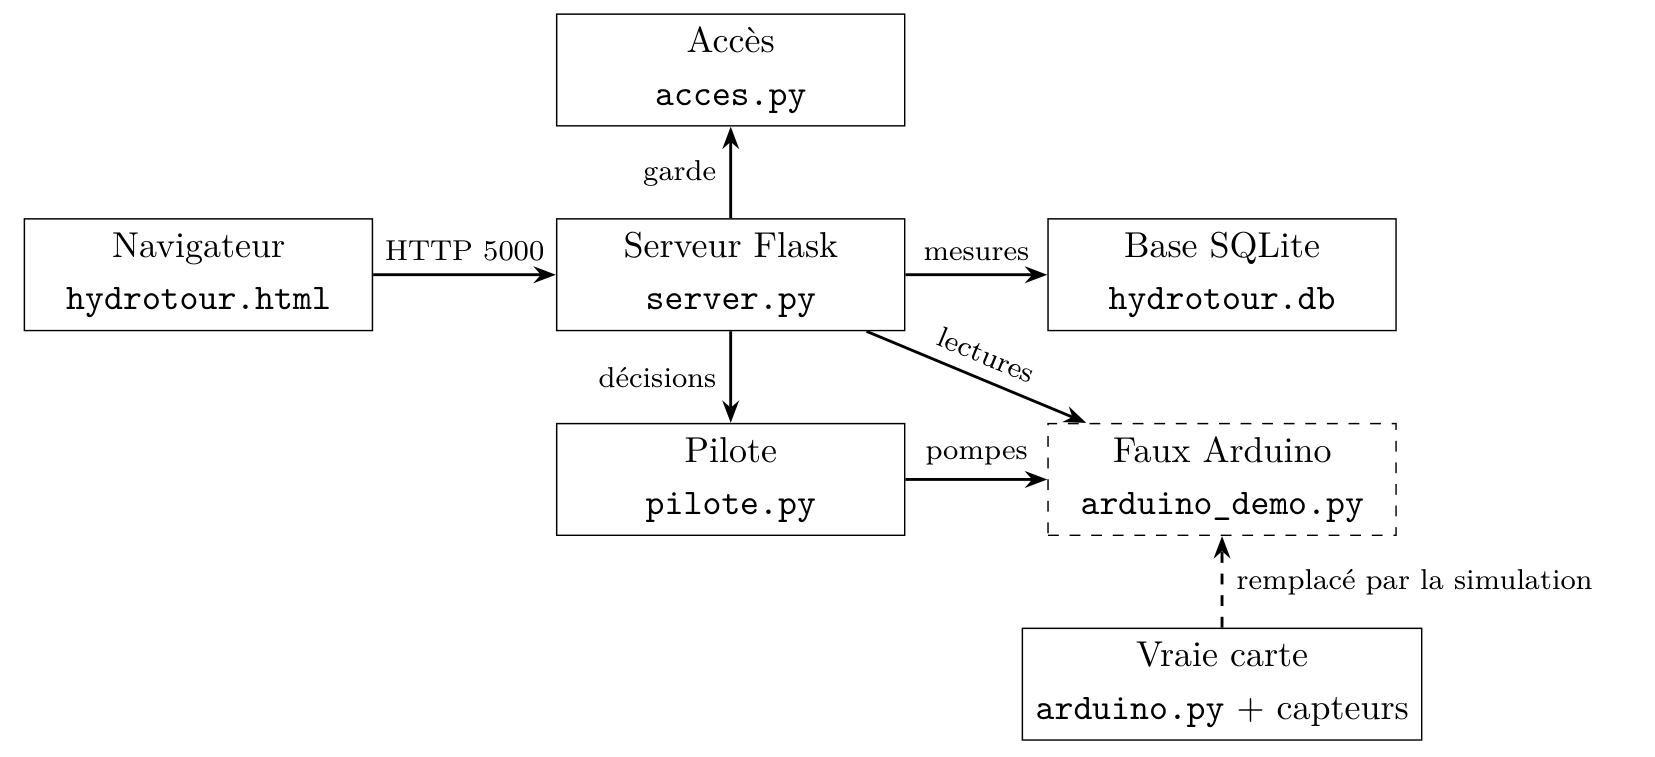
\includegraphics[width=0.85\textwidth]{img/inf/h_archi.png}
\caption{Architecture de la démo. Trait pointillé : l'élément qui remplace le matériel.}
\end{figure}

\subsubsection*{Les fichiers du dossier de démonstration}

Pour chaque fichier, je note s'il est copié tel quel, modifié ou nouveau. Je garde l'original intact dans \texttt{SERVEUR} : le dossier \texttt{DEMO} est une copie indépendante qu'on peut déplacer ou publier sans risque pour la vraie tour.

Le tableau suivant liste les fichiers de la démonstration.

\begin{table}[H]
\centering
\small
\begin{tabularx}{\textwidth}{|l|l|r|Y|}
\hline
\textbf{Fichier} & \textbf{État} & \textbf{Lignes} & \textbf{Rôle} \\
\hline
\texttt{hydrotour.html} & copié & 2097 & La page du dashboard \\
\hline
\texttt{pilote.py} & copié & 249 & Cycle de la pompe, batterie, dosage \\
\hline
\texttt{fausses\_mesures.py} & copié & 139 & Génère l'historique de départ \\
\hline
\texttt{server.py} & modifié & 544 & Serveur ; 22 lignes ajoutées \\
\hline
\texttt{acces.py} & modifié & 297 & Connexion ; 2 lignes ajoutées \\
\hline
\texttt{arduino\_demo.py} & nouveau & 134 & Simule la carte Arduino \\
\hline
\texttt{lancer\_demo.bat} & nouveau & 4 & Installe Flask et Pillow puis lance \\
\hline
\end{tabularx}
\caption{Fichiers de la démo.}
\end{table}

\subsubsection*{Un tour de mesure}

Le serveur répète le même tour toutes les \qty{10}{s}. Il lit les capteurs, convertit les valeurs brutes en grandeurs physiques, laisse le pilote décider, enregistre la ligne dans la base, puis attend. Comme la conversion se fait dans le serveur et non dans la carte, le faux Arduino doit renvoyer des valeurs brutes (millivolts, ohms) : c'est ce qui garantit que les conversions et l'étalonnage de la vraie tour sont aussi exercés.

L'organigramme suivant décrit la boucle de mesure du serveur.

\begin{figure}[H]
\centering
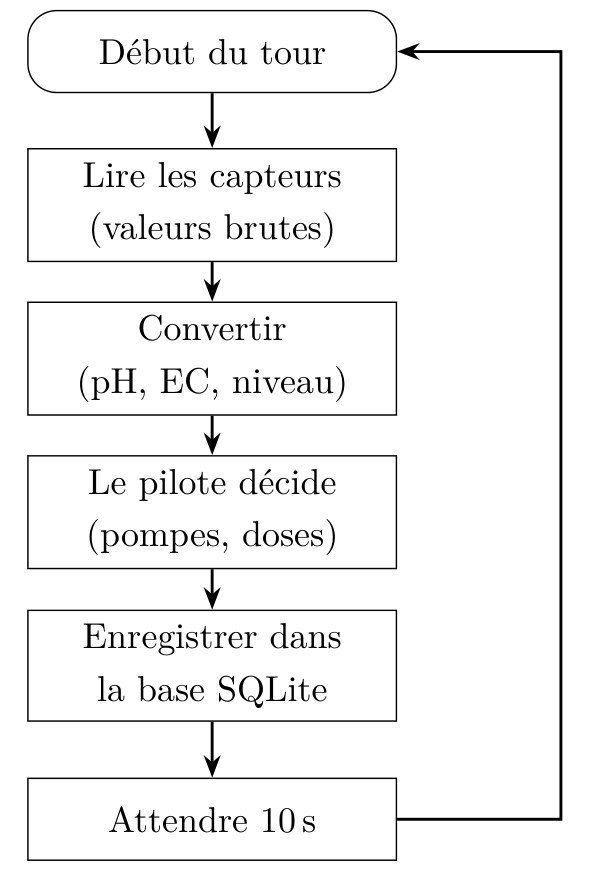
\includegraphics[width=0.42\textwidth]{img/inf/h_boucle.png}
\caption{Boucle de mesure du serveur (organigramme, ISO 5807).}
\end{figure}

% ---------------------------------------------------------------------
\Needspace{8\baselineskip}\subsection{Le faux Arduino}

Cette sous-partie explique d'abord le principe de la simulation. Elle présente ensuite les calculs qui transforment l'état simulé en valeurs brutes (pH, EC, niveau), puis le bilan d'énergie de la batterie, et enfin la façon dont les pompes agissent sur l'état.

\subsubsection*{Le principe}

Je cherche un modèle assez simple pour être écrit en cent lignes, mais assez réaliste pour que le pilote ait des décisions à prendre. L'état de la tour tient en quelques variables : le pH, l'EC, le niveau d'eau, la température de l'eau et la charge de la batterie. À chaque lecture, le temps réel écoulé depuis la dernière lecture fait avancer ces variables. Je plafonne ce temps à \qty{60}{s} pour qu'une mise en veille du PC ne fasse pas sauter la simulation.

Je choisis un temps réel et non un temps accéléré : le cycle de la pompe dure \qty{15}{min} en marche puis \qty{15}{min} à l'arrêt, et le soleil suit l'heure du PC. Une démonstration fidèle montre donc une vraie journée.

\begin{table}[H]
\centering
\small
\begin{tabularx}{\textwidth}{|l|l|Y|}
\hline
\textbf{Variable} & \textbf{Départ} & \textbf{Évolution sans intervention} \\
\hline
pH & 5,9 & monte de 0,002 par minute \\
\hline
EC & \qty{1150}{\micro S/cm} & baisse de \qty{0,6}{\micro S/cm} par minute \\
\hline
Niveau d'eau & \qty{78}{\percent} & baisse de \qty{0,03}{\percent} par minute, plus vite au soleil \\
\hline
Température de l'eau & \qty{21}{\celsius} & \qty{20,5}{\celsius} la nuit, jusqu'à \qty{22,3}{\celsius} en plein soleil \\
\hline
Batterie & \qty{70}{\percent} & selon le panneau et la consommation \\
\hline
\end{tabularx}
\caption{État simulé de la tour.}
\end{table}

Quand le niveau passe sous \qty{35}{\percent}, la simulation ajoute \qty{40}{\percent} d'eau et diminue l'EC de \qty{120}{\micro S/cm} : c'est le jardinier qui remet de l'eau. Sans ce geste, le pilote couperait la pompe sous \qty{15}{\percent} et la démonstration deviendrait vite immobile.

\subsubsection*{Du pH simulé à la tension}

Le serveur calcule le pH depuis la tension $U$ de la sonde. Pour que ce calcul soit exercé, la simulation doit faire le chemin inverse : à partir du pH voulu, elle renvoie la tension qui donnerait ce pH. Je pars de la droite d'étalonnage du serveur et j'isole $U$.

\naturecalc{simulation (valeurs du faux Arduino de la démonstration ; aucune mesure réelle)}
\begin{demonstration}[tension de la sonde pH]
\resultat{U \approx \qty{1693}{mV}}
Le serveur calcule le pH par la droite d'étalonnage, avec $U_7$ la tension dans le tampon pH 7 (en mV) et $U_4$ la tension dans le tampon pH 4 (en mV) :
\[
\mathrm{pH} = 7 + (U - U_7)\times\frac{4 - 7}{U_4 - U_7}
\]
Je soustrais 7 aux deux côtés :
\[
\mathrm{pH} - 7 = (U - U_7)\times\frac{4 - 7}{U_4 - U_7}
\]
Je multiplie par $\dfrac{U_4 - U_7}{4 - 7}$ pour isoler $U - U_7$ :
\[
U - U_7 = (\mathrm{pH} - 7)\times\frac{U_4 - U_7}{4 - 7}
\]
J'ajoute $U_7$ :
\[
U = U_7 + (\mathrm{pH} - 7)\times\frac{U_4 - U_7}{4 - 7}
\]
Avec un pH de $5{,}91$, $U_7 = \qty{1500}{mV}$ et $U_4 = \qty{2032}{mV}$ :
\begin{align*}
U &= \qty{1500}{mV} + (5{,}91 - 7)\times\frac{\qty{2032}{mV} - \qty{1500}{mV}}{4 - 7}\\
U &= \qty{1500}{mV} + (-1{,}09)\times\frac{\qty{532}{mV}}{-3}\\
U &= \qty{1500}{mV} + \qty{193,3}{mV}\\
U &\approx \qty{1693}{mV}
\end{align*}
Je m'arrête à l'unité du millivolt, qui est la précision de l'entrée analogique. Le journal du serveur affiche \qty{1694}{mV} : l'écart d'un millivolt vient du bruit aléatoire que la simulation ajoute exprès.
\end{demonstration}

\subsubsection*{De l'EC simulée à la tension}

La sonde d'EC donne une tension proportionnelle à la conductivité, corrigée de la température de l'eau. Le serveur ramène l'EC à \qty{25}{\celsius}. La simulation inverse cette conversion.

\naturecalc{simulation (valeurs du faux Arduino de la démonstration ; aucune mesure réelle)}
\begin{demonstration}[tension de la sonde EC]
\resultat{U_{EC} \approx \qty{173}{mV}}
Le serveur calcule l'EC (en \unit{\micro S/cm}) avec $U_{EC}$ la tension de la sonde (en mV), $K$ la constante de la sonde (sans unité, ici $1$) et $T$ la température de l'eau (en \unit{\celsius}) :
\[
EC = \frac{1000\times\dfrac{U_{EC}}{820\times 200}\times K}{1 + 0{,}0185\,(T - 25)}\times 1000
\]
Le numérateur est une conductivité en mS/cm, puis le facteur $1000$ final la convertit en \unit{\micro S/cm}. Je multiplie par le dénominateur et je divise par $1000$ à droite :
\[
EC\times\bigl(1 + 0{,}0185\,(T - 25)\bigr) = \frac{1000\times U_{EC}\times K\times 1000}{820\times 200}
\]
Puis j'isole $U_{EC}$ :
\[
U_{EC} = \frac{EC\times\bigl(1 + 0{,}0185\,(T - 25)\bigr)\times 820\times 200}{10^{6}\times K}
\]
Avec $EC = \qty{1140}{\micro S/cm}$, $T = \qty{21}{\celsius}$ et $K = 1$, je calcule d'abord le facteur de température :
\begin{align*}
1 + 0{,}0185\,(21 - 25) &= 1 - 0{,}074\\
&= 0{,}926
\end{align*}
Puis la tension :
\begin{align*}
U_{EC} &= \frac{1140\times 0{,}926\times 164\,000}{10^{6}}\ \unit{mV}\\
U_{EC} &= \frac{173{,}1\times 10^{6}}{10^{6}}\ \unit{mV}\\
U_{EC} &\approx \qty{173}{mV}
\end{align*}
Le journal du serveur affiche bien \qty{173}{mV}.
\end{demonstration}

\subsubsection*{Du niveau simulé à la résistance du ruban}

Le ruban eTape\ix{23} est une résistance qui diminue quand l'eau monte. Le serveur place le niveau entre deux étalonnages : \qty{2000}{\ohm} réservoir vide et \qty{400}{\ohm} réservoir plein.

\naturecalc{simulation (valeurs du faux Arduino de la démonstration ; aucune mesure réelle)}
\begin{demonstration}[résistance du ruban]
\resultat{R \approx \qty{752}{\ohm}}
Le serveur calcule le niveau $N$ (en \%) avec la résistance $R$ du ruban (en $\Omega$), $R_v$ la valeur à vide et $R_p$ la valeur à plein :
\[
N = \frac{R_v - R}{R_v - R_p}\times 100
\]
Je divise par $100$ et je multiplie par $R_v - R_p$ :
\[
\frac{N}{100}\times(R_v - R_p) = R_v - R
\]
J'isole $R$ :
\[
R = R_v - \frac{N}{100}\times(R_v - R_p)
\]
Avec $N = \qty{78}{\percent}$, $R_v = \qty{2000}{\ohm}$ et $R_p = \qty{400}{\ohm}$ :
\begin{align*}
R &= \qty{2000}{\ohm} - 0{,}78\times(\qty{2000}{\ohm} - \qty{400}{\ohm})\\
R &= \qty{2000}{\ohm} - 0{,}78\times\qty{1600}{\ohm}\\
R &= \qty{2000}{\ohm} - \qty{1248}{\ohm}\\
R &= \qty{752}{\ohm}
\end{align*}
Le journal affiche \qty{749}{\ohm} : l'écart vient du bruit ajouté à la mesure du niveau.
\end{demonstration}

\subsubsection*{La batterie et le soleil}

La batterie suit un bilan d'énergie. Le panneau fournit jusqu'à \qty{44}{W} (un panneau de \qty{55}{W} à \qty{80}{\percent} de rendement), multiplié par une courbe de soleil qui vaut zéro la nuit et un à midi. La consommation de base est celle du Raspberry, \qty{4,5}{W}. La pompe principale ajoute \qty{19}{W} et les doseuses \qty{6}{W}.

\naturecalc{simulation (valeurs du faux Arduino de la démonstration ; aucune mesure réelle)}
\begin{demonstration}[pente de décharge la nuit]
\resultat{\dfrac{\mathrm{d}\,\mathrm{SOC}}{\mathrm{d}t} \approx \qty{-30,6}{\percent/h}}
La charge $\mathrm{SOC}$ (en \%) varie avec la puissance nette $P$ (en W), positive en charge, et l'énergie $E$ de la batterie (en Wh) :
\[
\frac{\mathrm{d}\,\mathrm{SOC}}{\mathrm{d}t} = \frac{P}{E}\times 100
\]
L'énergie vaut la capacité $C$ (en Ah) fois la tension nominale $U_n$ (en V) :
\begin{align*}
E &= C\times U_n\\
E &= \qty{6}{Ah}\times\qty{12,8}{V}\\
E &= \qty{76,8}{Wh}
\end{align*}
La nuit, le panneau ne donne rien et la pompe tourne :
\[
P = -(\qty{4,5}{W} + \qty{19}{W}) = \qty{-23,5}{W}
\]
Je remplace :
\begin{align*}
\frac{\mathrm{d}\,\mathrm{SOC}}{\mathrm{d}t} &= \frac{\qty{-23,5}{W}}{\qty{76,8}{Wh}}\times 100\\
&= \qty{-0,306}{h^{-1}}\times 100\\
&\approx \qty{-30,6}{\percent/h}
\end{align*}
\end{demonstration}

Une nuit pompe en marche vide donc la batterie en quelques heures : le pilote doit couper la pompe sous \qty{30}{\percent}, ce que je vérifie dans les tests (9.5).

\subsubsection*{L'effet des pompes sur l'eau}

Pour que le pilote ait un retour, une pompe allumée change l'état simulé. Le débit d'une pompe péristaltique\ix{8} est de \qty{100}{mL/min}. J'admets que \qty{1}{mL} d'engrais ajoute \qty{6}{\micro S/cm} dans les \qty{40}{L} du réservoir, et que \qty{1}{mL} de solution pH- retire $0{,}03$ au pH.

\naturecalc{simulation (valeurs du faux Arduino de la démonstration ; aucune mesure réelle)}
\begin{demonstration}[effet d'une dose]
\resultat{\Delta EC \approx \qty{+30}{\micro S/cm}\quad\text{et}\quad \Delta\mathrm{pH} \approx -0{,}1}
Le volume versé $V$ (en mL) vaut le débit $Q$ (en mL/s) fois la durée $t$ (en s). Le débit vaut :
\begin{align*}
Q &= \frac{\qty{100}{mL}}{\qty{60}{s}}\\
Q &\approx \qty{1,67}{mL/s}
\end{align*}
Une dose d'engrais dure \qty{3}{s} (pour chacune des deux pompes, A puis B) :
\begin{align*}
V &= Q\times t\\
V &= \qty{1,67}{mL/s}\times\qty{3}{s}\\
V &\approx \qty{5}{mL}
\end{align*}
\begin{align*}
\Delta EC &= \qty{6}{\micro S/cm/mL}\times\qty{5}{mL}\\
\Delta EC &= \qty{30}{\micro S/cm}
\end{align*}
Une dose de pH- dure \qty{2}{s} :
\begin{align*}
V &= \qty{1,67}{mL/s}\times\qty{2}{s}\\
V &\approx \qty{3,3}{mL}\\
\Delta\mathrm{pH} &= -\qty{0,03}{mL^{-1}}\times\qty{3,3}{mL}\\
\Delta\mathrm{pH} &\approx -0{,}1
\end{align*}
\end{demonstration}

Le pH monte de $0{,}12$ par heure (soit $0{,}002\times 60$) et une dose le fait redescendre de $0{,}1$ : il faut en moyenne une dose par heure pour tenir le pH.

\begin{aretenir}
Le faux Arduino renvoie des valeurs brutes et réagit aux pompes. Le serveur et le pilote ne savent pas qu'il n'y a pas de matériel.
\end{aretenir}

% ---------------------------------------------------------------------
\Needspace{8\baselineskip}\subsection{Accès et premier lancement}

Cette sous-partie décrit d'abord le compte de démonstration et la sécurité conservée, ensuite le chemin d'une connexion, puis les routes du serveur, et enfin ce que le serveur prépare au tout premier lancement.

\subsubsection*{Le compte de démonstration}

Sur la vraie tour, le premier lancement crée un mot de passe provisoire au hasard, écrit dans un fichier. Pour une démonstration, ce n'est pas pratique : celui qui regarde doit connaître l'accès. Je remplace donc ce comportement par un compte fixe, et je l'écris sur la page de connexion.

Le tableau suivant donne l'accès à la démonstration.

\begin{table}[H]
\centering
\small
\begin{tabularx}{0.8\textwidth}{|l|Y|}
\hline
\textbf{Élément} & \textbf{Valeur} \\
\hline
Identifiant & \texttt{demo} \\
\hline
Mot de passe & \texttt{hydrotour-demo} \\
\hline
Adresse & \texttt{http://localhost:5000} \\
\hline
Port Internet & 5001 (publié par Tailscale\ix{20} Funnel\ix{20} si besoin) \\
\hline
\end{tabularx}
\caption{Accès à la démonstration.}
\end{table}

Je garde tout le reste de la sécurité. Le mot de passe n'est jamais stocké en clair mais sous forme d'une empreinte (fonction de hachage de Werkzeug). La session dure \qty{30}{jours}, le cookie est réservé au navigateur (HttpOnly) et refusé par les autres sites (SameSite=Lax), et le captcha est conservé. Les pages et l'API sont toutes protégées par une garde qui s'exécute avant chaque requête.

La figure suivante montre la page de connexion de la démonstration.

\begin{figure}[H]
\centering
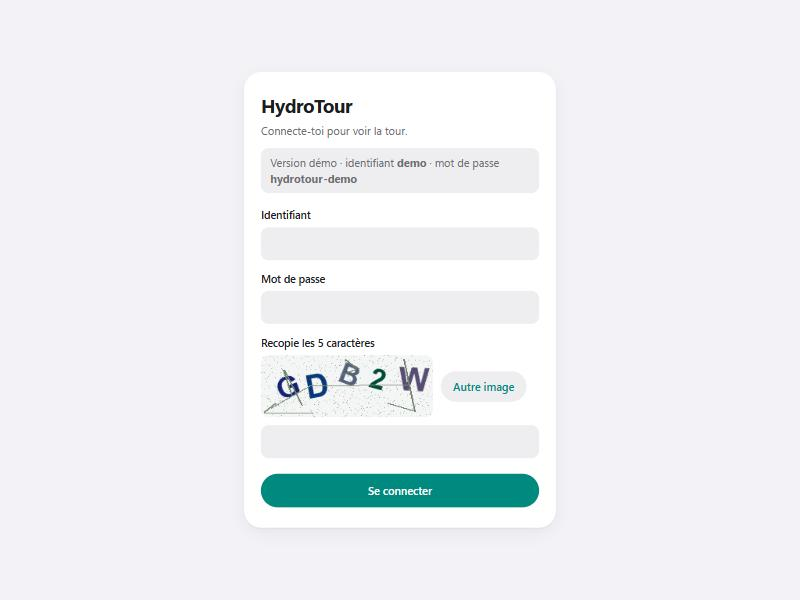
\includegraphics[width=0.75\textwidth]{img/inf/h_login.jpg}
\caption{Page de connexion de la démo, avec l'identifiant et le mot de passe rappelés et le captcha.}
\end{figure}

\subsubsection*{Le chemin d'une connexion}

Quand on ouvre la page, la garde regarde si la session est valide. Si elle ne l'est pas, elle renvoie vers la page de connexion. Le formulaire est accepté seulement si le captcha est juste, puis si le mot de passe correspond à l'empreinte. Je vérifie toujours le mot de passe, même quand l'identifiant est faux : le temps de réponse ne révèle donc pas si l'identifiant existe.

L'organigramme suivant décrit la connexion à la démonstration.

\begin{figure}[H]
\centering
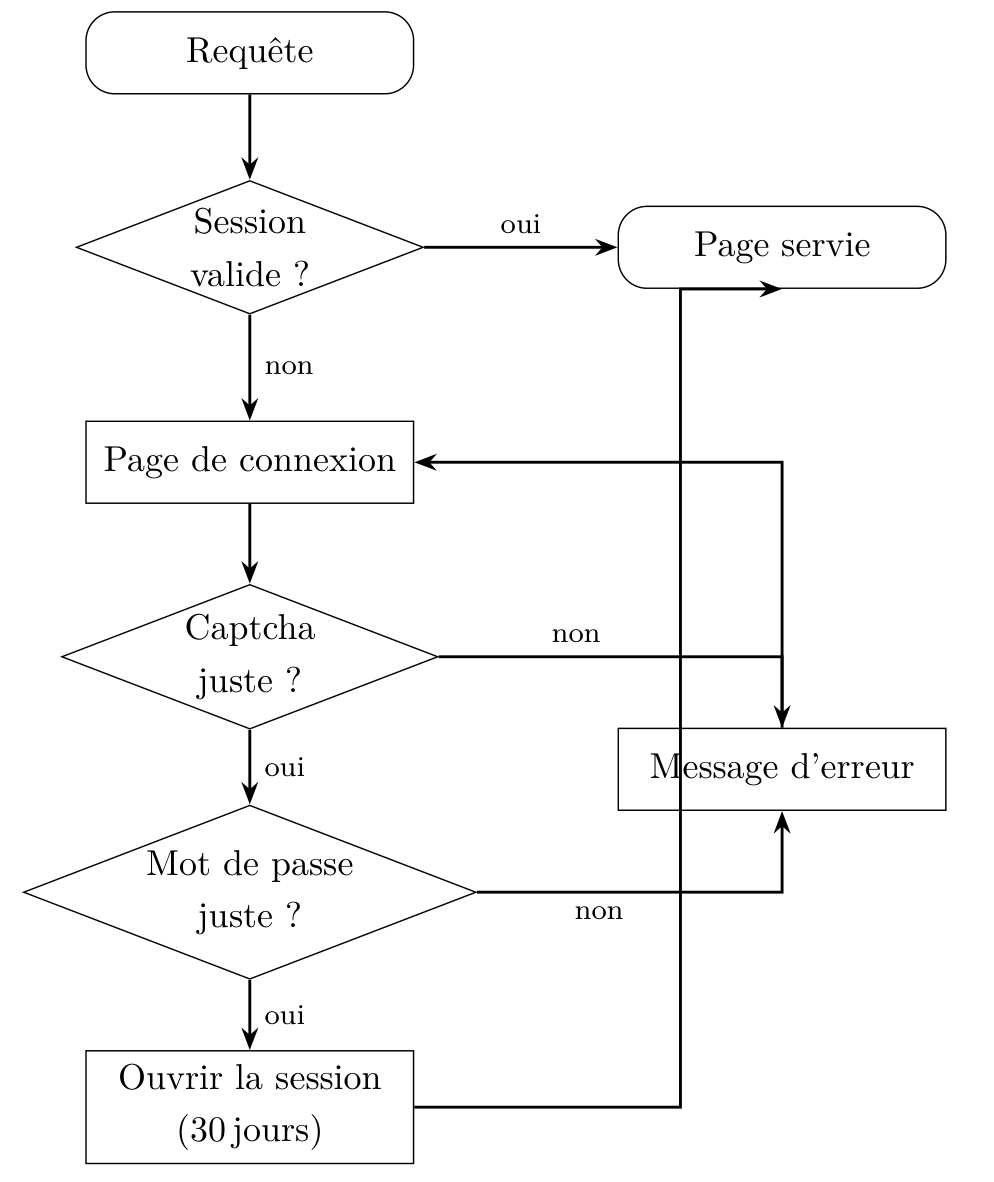
\includegraphics[width=0.6\textwidth]{img/inf/h_connexion.png}
\caption{Connexion à la démo (organigramme, ISO 5807).}
\end{figure}

\subsubsection*{Les routes du serveur}

Toutes les routes passent par la garde, sauf la page de connexion et l'image du captcha.

\begin{table}[H]
\centering
\small
\begin{tabularx}{\textwidth}{|l|l|Y|}
\hline
\textbf{Route} & \textbf{Méthode} & \textbf{Rôle} \\
\hline
\texttt{/} & GET & La page du dashboard \\
\hline
\texttt{/connexion} & GET, POST & Connexion (publique) \\
\hline
\texttt{/captcha.png} & GET & Image du captcha (publique) \\
\hline
\texttt{/api/latest} & GET & Dernière mesure, pompes, alertes, journal \\
\hline
\texttt{/api/history} & GET & Historique pour les courbes \\
\hline
\texttt{/api/pompe} & POST & Pompe principale ou dose à la main \\
\hline
\texttt{/api/pilotage} & GET, POST & Cycle, seuils de batterie, mode auto \\
\hline
\texttt{/api/culture} & GET, POST & Légume cultivé et date de plantation \\
\hline
\texttt{/api/stock} & GET, POST & Litres d'engrais A et B \\
\hline
\texttt{/api/batterie} & GET, POST & Capacité et tension de la batterie \\
\hline
\texttt{/api/etalonner} & POST & Étalonnage du pH et du niveau \\
\hline
\texttt{/api/acces} & GET, POST & Changer identifiant et mot de passe \\
\hline
\end{tabularx}
\caption{Routes de l'API.}
\end{table}

\subsubsection*{Le premier lancement}

Au premier lancement, la base est vide. Le serveur la remplit pour que la page ne soit pas vide à l'ouverture. Je génère trois jours d'historique, soit une mesure toutes les \qty{5}{min}, avec le script \texttt{fausses\_mesures.py} qui existait déjà. Je plante une tomate il y a \qty{30}{jours}, ce qui place la culture au stade floraison, avec les cibles de pH et d'EC correspondantes. Je mets enfin \qty{2}{L} dans chaque bidon d'engrais.

\naturecalc{simulation (valeurs du faux Arduino de la démonstration ; aucune mesure réelle)}
\begin{demonstration}[nombre de points d'historique]
\resultat{N = 864}
Le nombre $N$ de mesures (sans unité) vaut la durée $D$ (en h) divisée par le pas $p$ (en h) :
\[
N = \frac{D}{p}
\]
Avec $D = \qty{72}{h}$ et $p = \qty{5}{min} = \tfrac{1}{12}\,\unit{h}$ :
\begin{align*}
N &= \frac{\qty{72}{h}}{\frac{1}{12}\,\unit{h}}\\
N &= 72\times 12\\
N &= 864
\end{align*}
Le serveur en relève \num{870} dans l'historique, car quelques mesures en direct se sont ajoutées après le démarrage.
\end{demonstration}

Cette préparation ne se fait qu'une fois : si la base contient déjà des mesures, le serveur n'y touche pas.

% ---------------------------------------------------------------------
\Needspace{8\baselineskip}\subsection{Tests et résultats}

Cette sous-partie présente d'abord les vérifications que je fais, ensuite les données produites par la démonstration en tableaux et en courbes, puis ce que je constate et les limites. Elle se termine par le mode d'emploi pour lancer la démonstration.

\subsubsection*{Les vérifications}

Je teste d'abord que la connexion est bien exigée, puis que chaque route répond une fois la session ouverte. Pour ouvrir la session sans passer par le formulaire, j'utilise le client de test de Flask, qui écrit directement la session côté serveur. Je ne résous pas le captcha moi-même : c'est une protection anti-robot, et le formulaire de connexion reste à essayer à la main.

Le tableau suivant donne les résultats des essais.

\begin{table}[H]
\centering
\small
\begin{tabularx}{\textwidth}{|l|Y|l|}
\hline
\textbf{Essai} & \textbf{Attendu} & \textbf{Obtenu} \\
\hline
\texttt{/api/latest} sans session & refusé (401) & 401 \\
\hline
\texttt{/} sans session & redirigé vers \texttt{/connexion} & 302 \\
\hline
\texttt{/api/latest} avec session & données (200) & 200 \\
\hline
\texttt{/api/history} 72 h & environ 870 points & 870 \\
\hline
\texttt{/api/culture} & tomate, floraison & oui \\
\hline
\texttt{/api/stock} & 2 L et 2 L & oui \\
\hline
\texttt{/api/pilotage} & réglages (200) & 200 \\
\hline
\texttt{/} avec session & page complète & \qty{130782}{octets} \\
\hline
Bon mot de passe & accepté & oui \\
\hline
Mauvais mot de passe & refusé & oui \\
\hline
\end{tabularx}
\caption{Résultats des essais.}
\end{table}

\subsubsection*{La dernière mesure}

Voici la mesure renvoyée par \texttt{/api/latest} au moment des essais, avec l'état des pompes. La pompe principale tourne, car le cycle de \qty{15}{min} la met en marche, et les doseuses attendent que l'eau soit mélangée.

\begin{table}[H]
\centering
\small
\begin{tabularx}{0.7\textwidth}{|l|r|l|}
\hline
\textbf{Grandeur} & \textbf{Valeur} & \textbf{Unité} \\
\hline
pH & 5,91 & -- \\
\hline
EC & 1155 & \unit{\micro S/cm} \\
\hline
Température de l'eau & 20,5 & \unit{\celsius} \\
\hline
Température de l'air & 26,2 & \unit{\celsius} \\
\hline
Humidité & 75 & \unit{\percent} \\
\hline
Pression & 1012,7 & \unit{hPa} \\
\hline
Niveau d'eau & 77,9 & \unit{\percent} \\
\hline
Lumière & 0 & \unit{\percent} \\
\hline
Batterie (tension) & 12,967 & \unit{V} \\
\hline
Batterie (courant) & $-1{,}812$ & \unit{A} \\
\hline
Batterie (puissance) & $-23{,}5$ & \unit{W} \\
\hline
Batterie (charge) & 69,5 & \unit{\percent} \\
\hline
\end{tabularx}
\caption{Dernière mesure de la démo.}
\end{table}

\naturecalc{simulation (valeurs du faux Arduino de la démonstration ; aucune mesure réelle)}
\begin{demonstration}[courant de la batterie]
\resultat{I \approx \qty{-1,812}{A}}
La puissance $P$ (en W) vaut la tension $U$ (en V) fois le courant $I$ (en A) :
\[
P = U\times I
\]
J'isole $I$ :
\[
I = \frac{P}{U}
\]
\begin{align*}
I &= \frac{\qty{-23,5}{W}}{\qty{12,967}{V}}\\
I &\approx \qty{-1,812}{A}
\end{align*}
Cette valeur correspond à la mesure du tableau.
\end{demonstration}

\subsubsection*{Les statistiques sur 72 heures}

Je relève le minimum, le maximum et la moyenne de chaque grandeur sur l'historique de trois jours.

Le tableau suivant donne les statistiques de l'historique.

\begin{table}[H]
\centering
\small
\begin{tabularx}{\textwidth}{|l|r|r|r|l|}
\hline
\textbf{Grandeur} & \textbf{Minimum} & \textbf{Maximum} & \textbf{Moyenne} & \textbf{Unité} \\
\hline
pH & 5,82 & 6,02 & 5,92 & -- \\
\hline
EC & 1012 & 1184 & 1101 & \unit{\micro S/cm} \\
\hline
Eau & 20,3 & 22,1 & 20,97 & \unit{\celsius} \\
\hline
Air & 21,7 & 30,5 & 25,99 & \unit{\celsius} \\
\hline
Humidité & 66 & 93 & 79,99 & \unit{\percent} \\
\hline
Lumière & 0 & 99 & 22,5 & \unit{\percent} \\
\hline
Niveau & 65 & 83 & 74,9 & \unit{\percent} \\
\hline
Pression & 1011,4 & 1014,6 & 1013,0 & \unit{hPa} \\
\hline
Tension batterie & 12,61 & 13,84 & 13,01 & \unit{V} \\
\hline
Courant batterie & $-1{,}86$ & 2,83 & $-0{,}43$ & \unit{A} \\
\hline
Puissance batterie & $-23{,}5$ & 38,88 & $-5{,}28$ & \unit{W} \\
\hline
Charge batterie & 0 & 100 & 35,4 & \unit{\percent} \\
\hline
\end{tabularx}
\caption{Statistiques de l'historique (870 mesures).}
\end{table}

Le pH reste entre $5{,}82$ et $6{,}02$, donc dans la cible de la tomate à la floraison ($5{,}8$ à $6{,}3$). L'EC, elle, reste entre \qty{1012}{\micro S/cm} et \qty{1184}{\micro S/cm}, sous la cible de \qty{2000}{\micro S/cm} à \qty{2400}{\micro S/cm} : le pilote voudra donc doser de l'engrais en direct, ce qui rend la démonstration vivante.

\subsubsection*{Les courbes}

Je trace quatre grandeurs sur les \qty{72}{h} d'historique, une mesure toutes les \qty{30}{min}. Les données viennent directement de la route \texttt{/api/history}.

\begin{figure}[H]
\centering
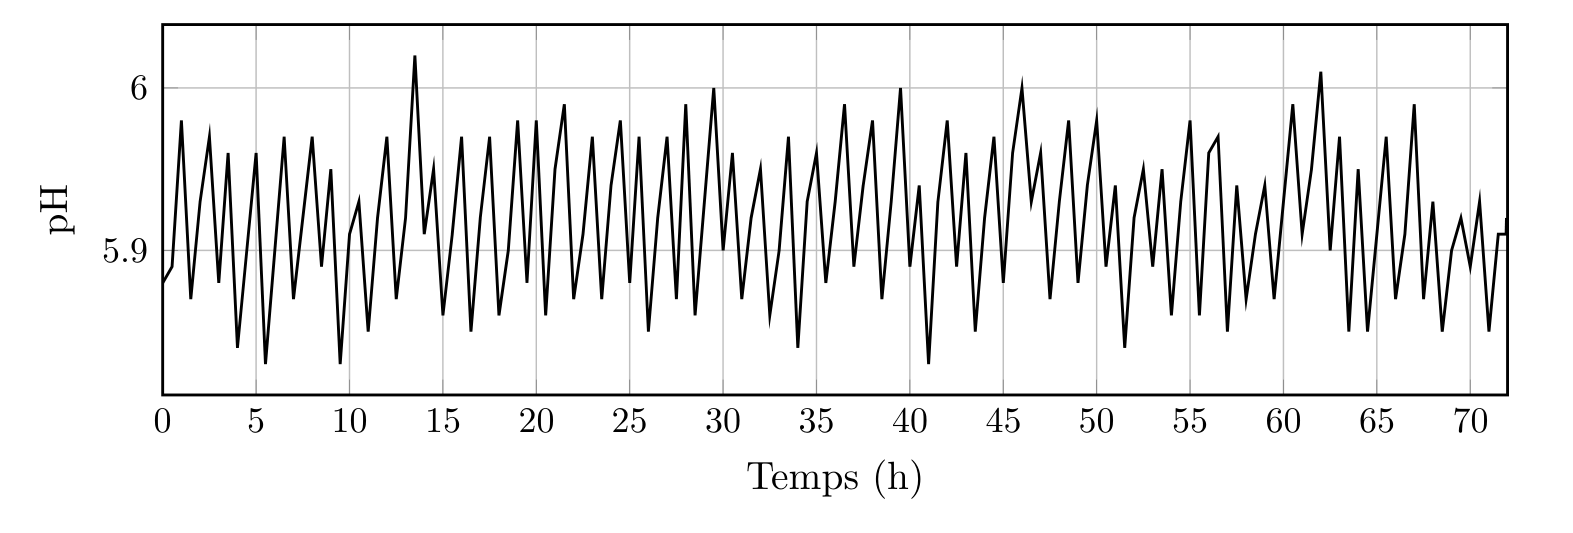
\includegraphics[width=0.9\textwidth]{img/inf/h_c_ph.png}
\caption{pH de la solution sur 72 h.}
\end{figure}

\begin{figure}[H]
\centering
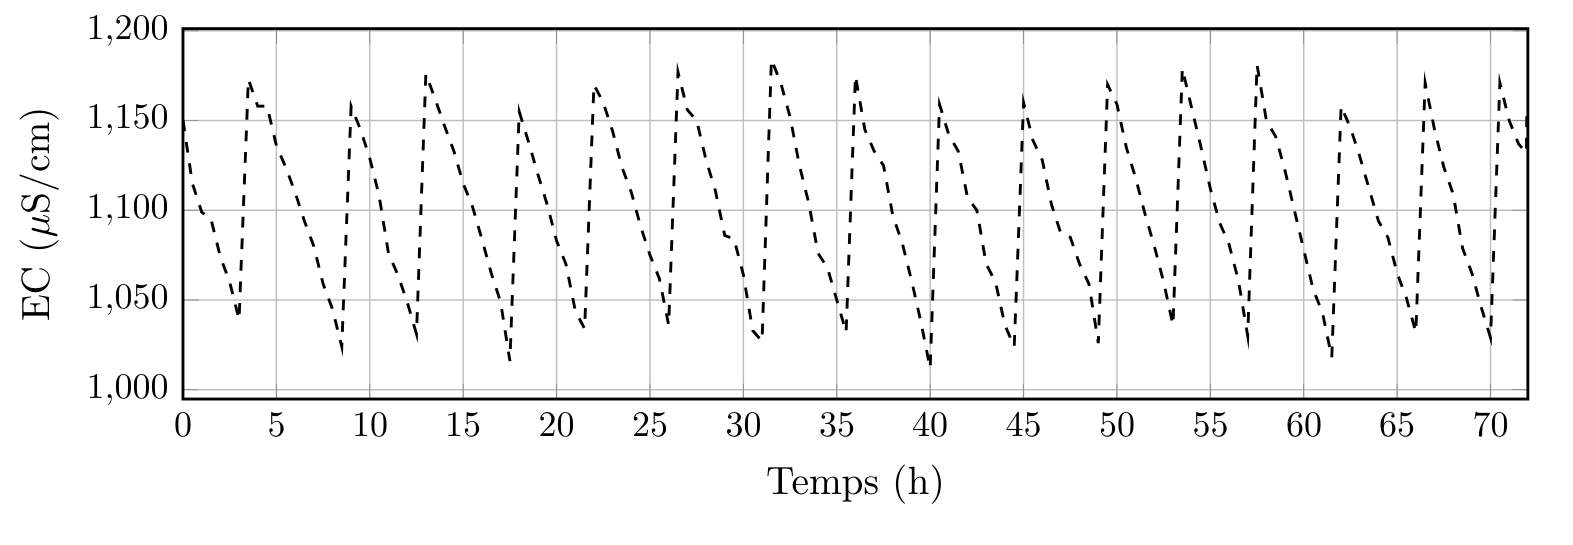
\includegraphics[width=0.9\textwidth]{img/inf/h_c_ec.png}
\caption{Conductivité de la solution sur 72 h.}
\end{figure}

\begin{figure}[H]
\centering
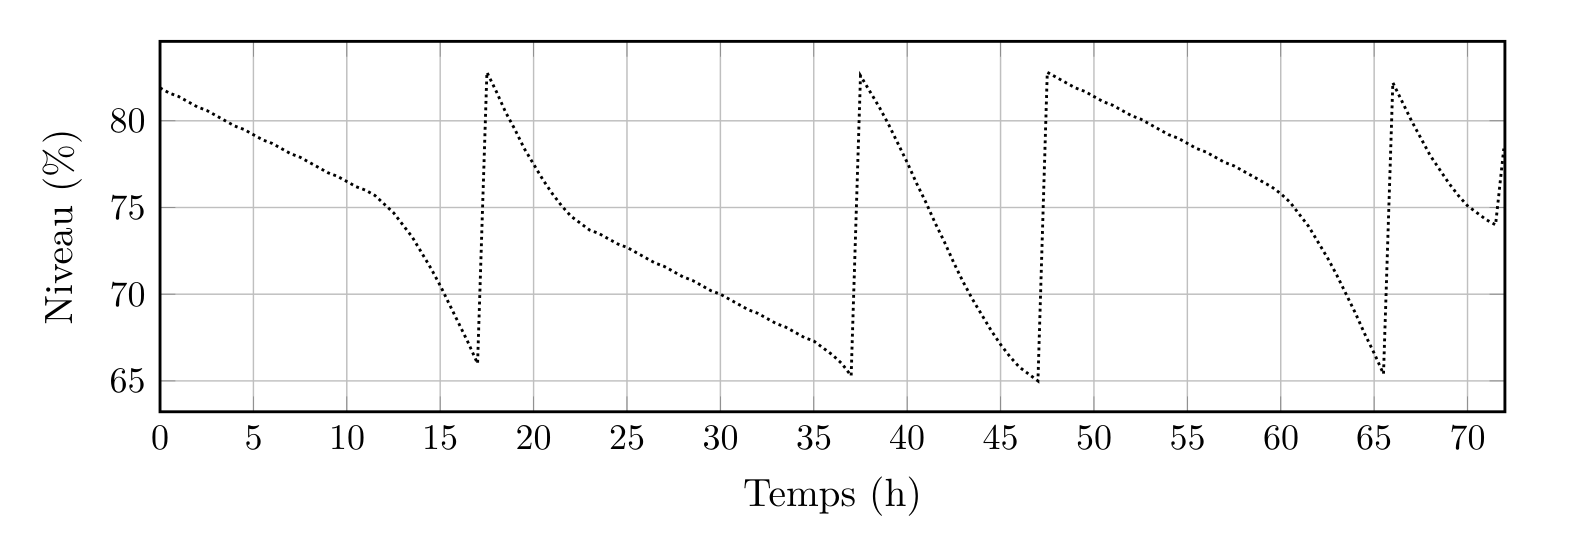
\includegraphics[width=0.9\textwidth]{img/inf/h_c_niv.png}
\caption{Niveau d'eau du réservoir sur 72 h.}
\end{figure}

\begin{figure}[H]
\centering
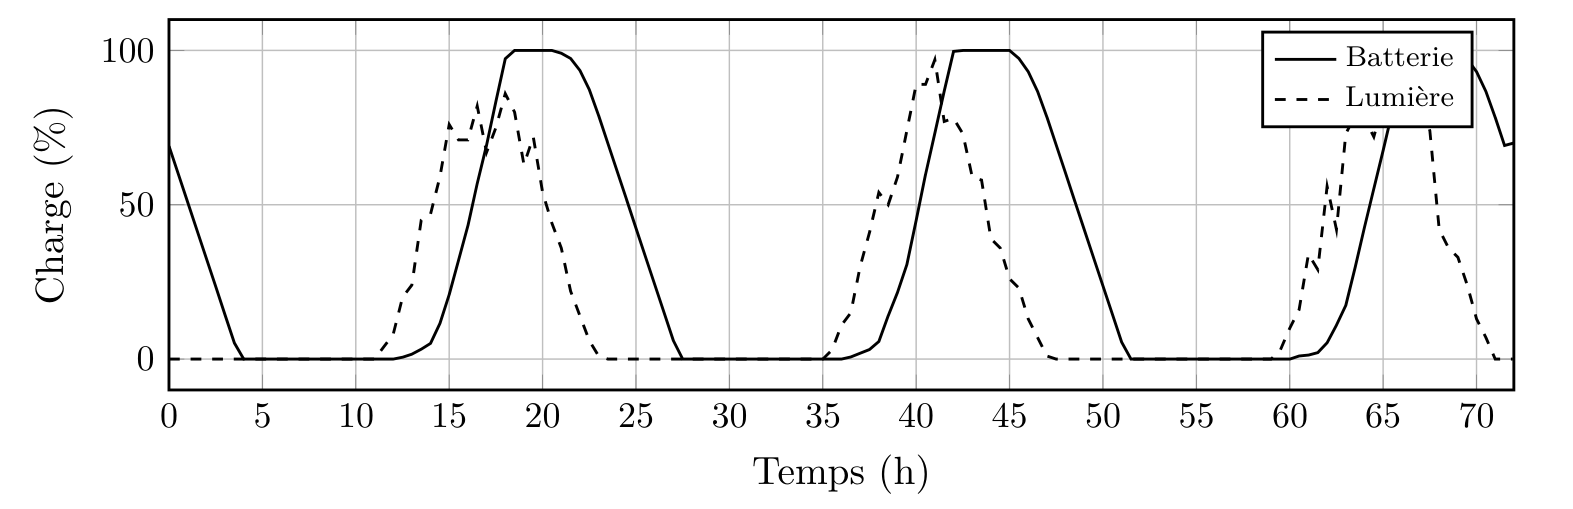
\includegraphics[width=0.9\textwidth]{img/inf/h_c_bat.png}
\caption{Charge de la batterie et lumière sur 72 h.}
\end{figure}

\subsubsection*{Ce que je constate et les limites}

Je constate d'abord que les courbes ont l'allure attendue : la lumière dessine un jour et une nuit, la batterie se charge le jour et se vide la nuit, le pH remonte puis redescend après chaque dose, et le niveau s'abaisse plus vite au soleil.

Deux limites sont à connaître. La première concerne l'historique : le script \texttt{fausses\_mesures.py} le génère sans pilote, avec une pompe qui tourne un quart d'heure sur deux, sans coupure de batterie. La charge descend donc jusqu'à \qty{0}{\percent} dans le passé, alors que le pilote en direct coupe la pompe à \qty{30}{\percent}. Il y a un saut entre la fin de l'historique et la première mesure en direct. La seconde limite concerne la connexion : je n'ai pas essayé moi-même le formulaire complet avec le captcha, car recopier un captcha est une action réservée à une personne. Les captures du dashboard de la sous-partie suivante viennent donc d'une copie statique de la page, qui embarque les données réelles du serveur de démo.

\begin{attention}
La démo tourne en temps réel : pour voir le pilote couper la pompe sous \qty{30}{\percent} ou doser de l'engrais, il faut la laisser tourner plusieurs heures, ou régler les seuils dans Paramètres.
\end{attention}

\subsubsection*{Lancer la démonstration}

Sur un ordinateur avec Python, j'ouvre le dossier \texttt{HYDROCODE/DEMO} et je lance \texttt{lancer\_demo.bat}. Ce fichier installe Flask et Pillow, puis démarre le serveur. J'ouvre ensuite \texttt{http://localhost:5000} et je me connecte avec \texttt{demo} et \texttt{hydrotour-demo}. Pour la rendre visible depuis Internet, il suffirait de publier le port 5001 avec Tailscale\ix{20} Funnel\ix{20}, comme pour la vraie tour : je ne l'ai pas fait.

\begin{aretenir}
La démo reprend le vrai serveur, le vrai pilote, la vraie page et la vraie sécurité. Elle fonctionne sans matériel, avec un compte fixe, et réagit comme la tour quand les pompes s'allument.
\end{aretenir}

% ---------------------------------------------------------------------
\Needspace{8\baselineskip}\subsection{Dashboard en ligne et captures}

Cette sous-partie explique d'abord comment je fabrique une copie statique du dashboard qui embarque les données de la démo. Elle présente ensuite les captures de chaque vue en lisant les valeurs qu'elles affichent, puis décrit la version publiée en ligne, avec ce qu'elle fait et ce qu'elle ne fait pas.

\subsubsection*{Une copie statique qui garde les données réelles}

Je cherche à obtenir des captures et une version en ligne sans dépendre du captcha ni d'un serveur qui tourne. La page \texttt{hydrotour.html} lit ses données avec la fonction \texttt{fetch} sur les routes \texttt{/api/...}. Je ne change donc rien à la page : j'ajoute avant elle un petit script qui remplace \texttt{fetch}. Ce script répond aux mêmes routes avec des données que j'ai relevées une fois sur le serveur de démo (client de test de Flask, session ouverte côté serveur). La page croit parler au serveur et passe en mode « En direct », comme sur la tour.

Le tableau suivant liste les routes imitées par la copie statique.

\begin{table}[H]
\centering
\small
\begin{tabularx}{\textwidth}{|l|Y|}
\hline
\textbf{Route imitée} & \textbf{Réponse du script} \\
\hline
\texttt{/api/latest} & dernière mesure, pompes, alertes, journal \\
\hline
\texttt{/api/history} & 942 mesures, filtrées sur la durée demandée \\
\hline
\texttt{/api/pilotage} & cycle 15/15 min, coupure \qty{30}{\percent}, reprise \qty{35}{\percent} \\
\hline
\texttt{/api/culture} & tomate plantée le 12 octobre \\
\hline
\texttt{/api/stock} & \qty{2}{L} d'engrais A et \qty{2}{L} d'engrais B \\
\hline
\texttt{/api/batterie} & \qty{6}{Ah}, \qty{12,8}{V} \\
\hline
\texttt{/api/pompe} (POST) & change l'état de la pompe en mémoire \\
\hline
\texttt{/api/acces}, \texttt{/api/etalonner} & refusés : pas de serveur derrière \\
\hline
\end{tabularx}
\caption{Routes imitées par la copie statique.}
\end{table}

Les mesures ont été prises à un moment précis, mais la page affiche « dernières 24 h » par rapport à l'instant présent. Je décale donc toutes les dates à chaque ouverture, pour que la dernière mesure tombe sur l'instant où la page s'ouvre.

\naturecalc{simulation (valeurs du faux Arduino de la démonstration ; aucune mesure réelle)}
\begin{demonstration}[décalage des dates]
\resultat{t'_i = t_i + \Delta\quad\text{avec}\quad \Delta = t_{\text{maintenant}} - t_{\text{dernière}}}
Je note $t_i$ la date de la mesure numéro $i$ dans les données relevées (en secondes depuis une origine fixe), $t_{\text{dernière}}$ la date de la dernière mesure et $t_{\text{maintenant}}$ l'instant d'ouverture de la page. Je veux que la dernière mesure tombe sur l'instant présent :
\[
t'_{\text{dernière}} = t_{\text{maintenant}}
\]
Je cherche un décalage $\Delta$ (en secondes) identique pour toutes les mesures, pour garder les écarts entre elles. Je pose :
\[
t'_i = t_i + \Delta
\]
Je l'écris pour la dernière mesure :
\begin{align*}
t'_{\text{dernière}} &= t_{\text{dernière}} + \Delta\\
t_{\text{maintenant}} &= t_{\text{dernière}} + \Delta\\
\Delta &= t_{\text{maintenant}} - t_{\text{dernière}}
\end{align*}
L'écart entre deux mesures est conservé :
\begin{align*}
t'_{i+1} - t'_i &= (t_{i+1} + \Delta) - (t_i + \Delta)\\
&= t_{i+1} - t_i
\end{align*}
Pour la vue 24 h, la page garde les mesures de date $t'_i \geq t_{\text{maintenant}} - \qty{24}{h}$. Avec une mesure toutes les \qty{5}{min} :
\begin{align*}
N &= \frac{\qty{24}{h}}{\frac{1}{12}\,\unit{h}}\\
N &= 24\times 12\\
N &= 288
\end{align*}
Les $942$ mesures relevées se décomposent en $864$ points d'historique et $942 - 864 = 78$ mesures en direct, soit $78\times\qty{10}{s} = \qty{780}{s} = \qty{13}{min}$ de fonctionnement du serveur avant le relevé.
\end{demonstration}

\subsubsection*{Les captures du dashboard}

Je prends moi-même les captures avec le navigateur intégré de l'application, dans une fenêtre de \qty{800}{px} de large. Chaque capture est lue en regard des données de la démo : les valeurs affichées sont celles du serveur, pas des valeurs écrites à la main.

La première vue est celle des mesures. Elle affiche en haut l'état de la liaison (« En direct »), puis une alarme quand une grandeur sort de sa cible. Ici l'alarme porte sur l'EC : \qty{1144}{\micro S/cm} contre une cible de \qty{2000}{\micro S/cm} à \qty{2400}{\micro S/cm}, ce qui correspond aux statistiques et explique pourquoi le pilote dose de l'engrais. Le pH, $5{,}94$, est dans sa cible de $5{,}8$ à $6{,}3$.

La figure suivante montre la vue Mesures, avec le bac et la solution nutritive.

\begin{figure}[H]
\centering
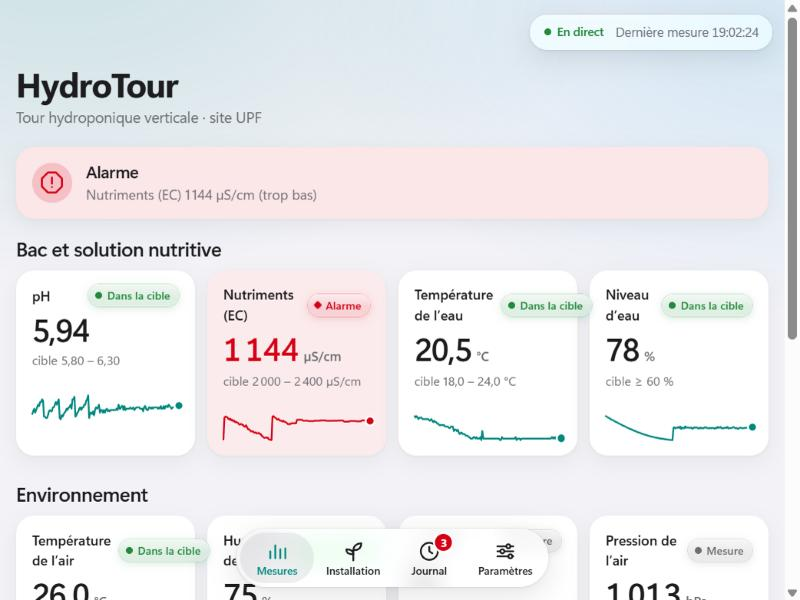
\includegraphics[width=0.8\textwidth]{img/inf/h_mesures.jpg}
\caption{Vue Mesures : bac et solution nutritive. L'EC est en alarme, le pH, la température de l'eau et le niveau sont dans leur cible.}
\end{figure}

Plus bas, la vue montre l'environnement (air, humidité, lumière, pression) et la batterie. Je contrôle l'autonomie affichée : la batterie contient \qty{49}{Wh} sur \qty{77}{Wh} et débite \qty{23,5}{W} (pompe et Raspberry).

\begin{figure}[H]
\centering
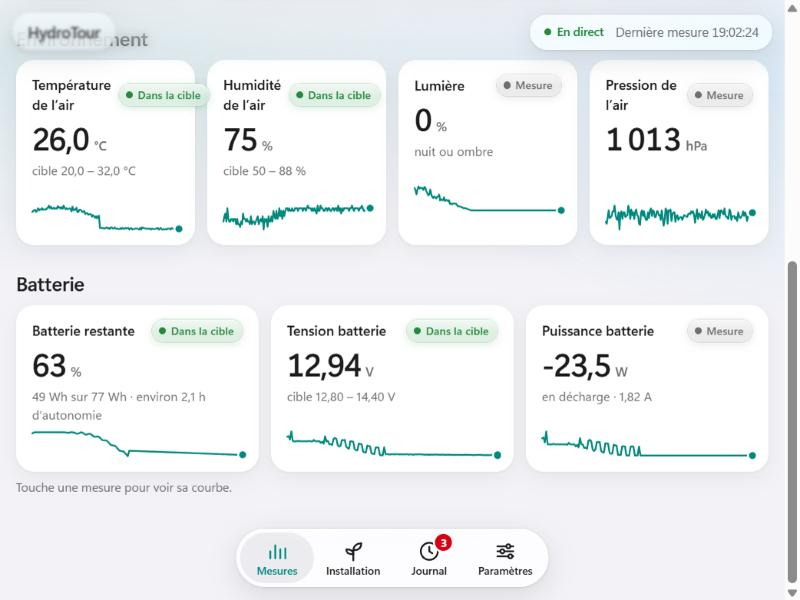
\includegraphics[width=0.8\textwidth]{img/inf/h_env.jpg}
\caption{Vue Mesures : environnement et batterie, avec l'autonomie estimée.}
\end{figure}

\naturecalc{simulation (valeurs du faux Arduino de la démonstration ; aucune mesure réelle)}
\begin{demonstration}[autonomie de la batterie]
\resultat{t \approx \qty{2,1}{h}}
L'autonomie $t$ (en h) vaut l'énergie restante $E$ (en Wh) divisée par la puissance de décharge $P$ (en W) :
\[
t = \frac{E}{P}
\]
L'énergie restante est la charge $\mathrm{SOC}$ (en \%) de l'énergie totale $E_0 = \qty{76,8}{Wh}$ :
\begin{align*}
E &= \frac{\mathrm{SOC}}{100}\times E_0\\
E &= 0{,}63\times\qty{76,8}{Wh}\\
E &\approx \qty{48,4}{Wh}
\end{align*}
La page arrondit la charge à partir d'une valeur un peu plus haute, ce qui donne \qty{49}{Wh}. Avec $P = \qty{23,5}{W}$ :
\begin{align*}
t &= \frac{\qty{49}{Wh}}{\qty{23,5}{W}}\\
t &\approx \qty{2,09}{h}
\end{align*}
La page affiche « environ 2,1 h ». Le courant affiché se contrôle de la même façon :
\[
\frac{\qty{23,5}{W}}{\qty{12,94}{V}} \approx \qty{1,82}{A}
\]
\end{demonstration}

La vue Installation montre la tour en trois dimensions, avec les plantes, le panneau solaire et le bac. Elle indique le stade de la culture (« Floraison, jour 30 »), qui vient de la date de plantation envoyée au serveur.

\begin{figure}[H]
\centering
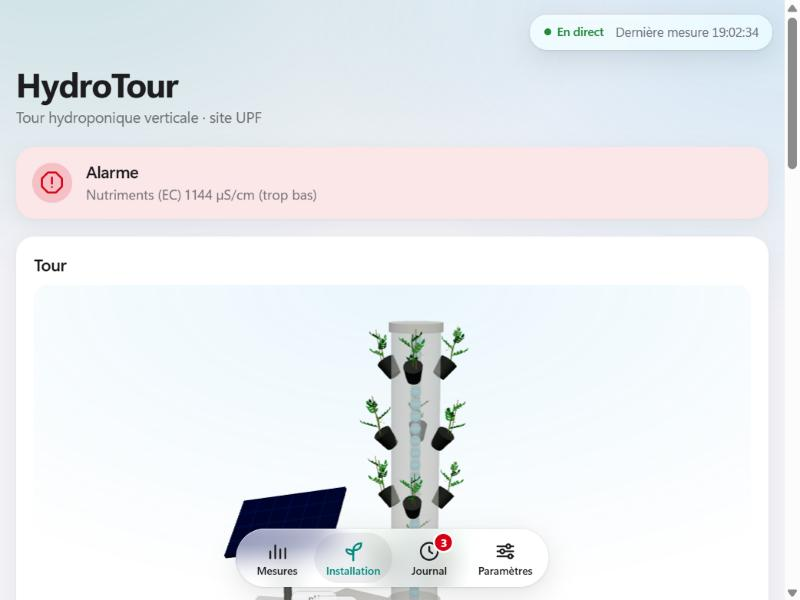
\includegraphics[width=0.8\textwidth]{img/inf/h_tour.jpg}
\caption{Vue Installation : la tour en 3D.}
\end{figure}

Sous la tour, le calendrier de la culture (tomate cerise, plantée le 12 octobre) colore chaque jour selon son stade. Je vérifie le numéro de jour : du 12 octobre au 11 novembre, il y a $19 + 11 = 30$ jours (les 19 jours restants d'octobre après le 12, puis 11 jours de novembre).

\begin{figure}[H]
\centering
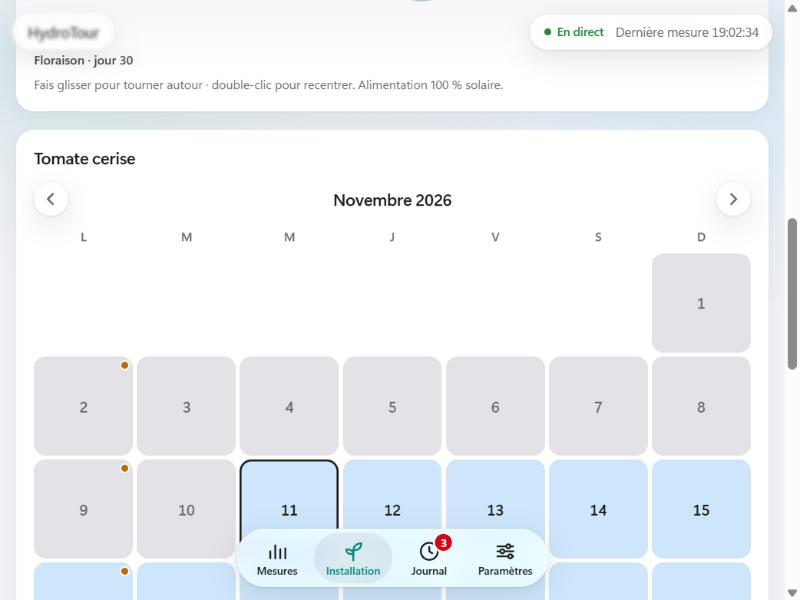
\includegraphics[width=0.8\textwidth]{img/inf/h_calendrier.jpg}
\caption{Vue Installation : calendrier de la culture.}
\end{figure}

La vue Journal liste les derniers événements du pilote (démarrage de la pompe, doses d'engrais et de pH-) puis un tableau des données récoltées par jour, sur 24 h, 7 j ou 30 j. Le tableau indique 942 mesures du 8 au 11 novembre.

\begin{figure}[H]
\centering
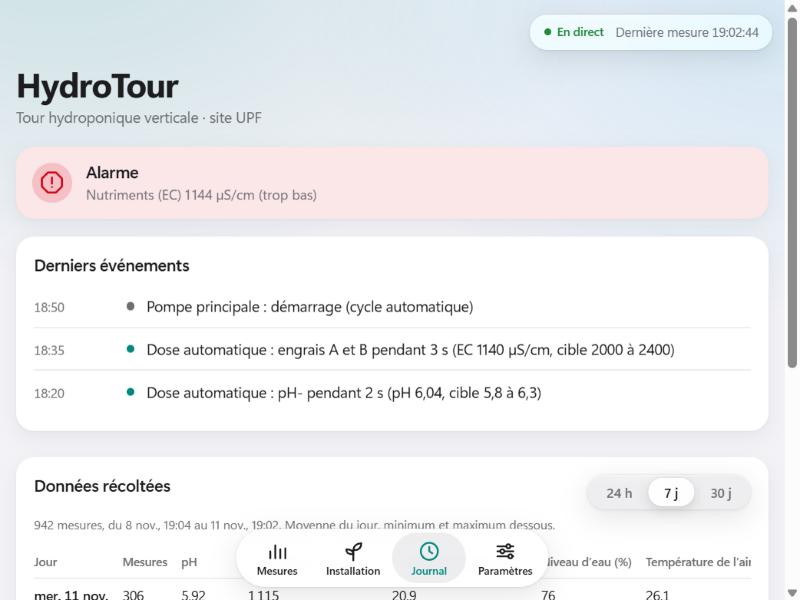
\includegraphics[width=0.8\textwidth]{img/inf/h_journal.jpg}
\caption{Vue Journal : événements du pilote et données récoltées.}
\end{figure}

\begin{attention}
Les trois lignes du journal de cette capture sont des exemples que j'ai écrits dans le style du pilote : le serveur utilisé pour le relevé n'avait pas encore produit d'événement. Les mesures et les cibles, elles, viennent de la démo.
\end{attention}

Enfin la vue Paramètres regroupe l'accès, le légume, la batterie, le pilotage et l'étalonnage. L'accès montre l'identifiant \texttt{demo}. Le pilotage affiche les valeurs par défaut du pilote : marche \qty{15}{min}, arrêt \qty{15}{min}, coupure de la batterie à \qty{30}{\percent} et reprise à \qty{35}{\percent}, soit le conseil du programme.

\begin{figure}[H]
\centering
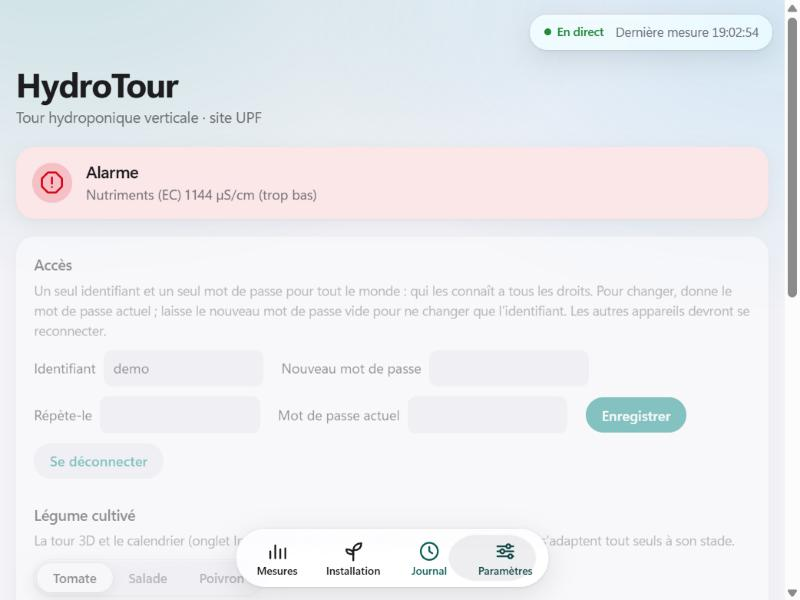
\includegraphics[width=0.8\textwidth]{img/inf/h_param.jpg}
\caption{Vue Paramètres : accès à la démo.}
\end{figure}

\begin{figure}[H]
\centering
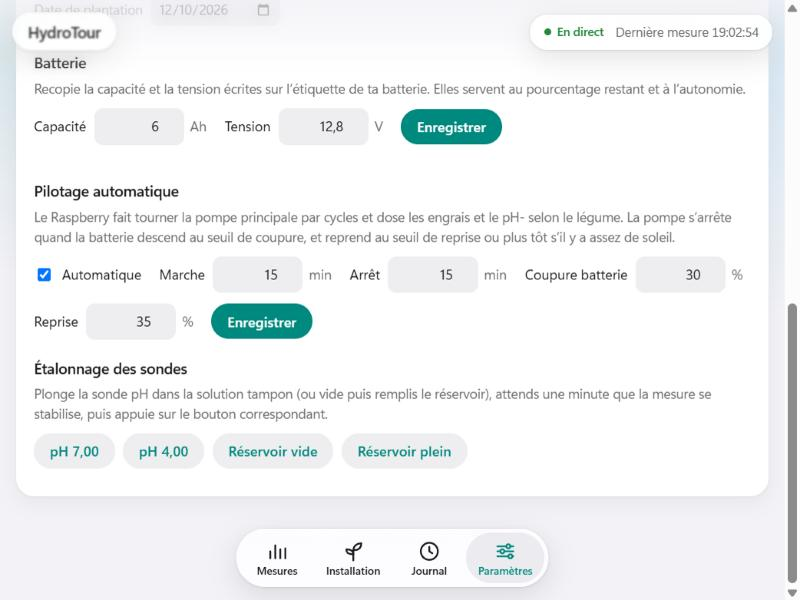
\includegraphics[width=0.8\textwidth]{img/inf/h_param2.jpg}
\caption{Vue Paramètres : batterie, pilotage automatique et étalonnage des sondes.}
\end{figure}

\subsubsection*{Le dashboard publié en artéfact}

Je publie le dashboard comme artéfact, une page web hébergée qui s'ouvre dans un navigateur sans rien installer. Depuis le 20 novembre 2026, la page publiée n'est plus une copie statique : c'est le fichier \texttt{hydrotour.html} de la tour, auquel j'ajoute une seule ligne qui pose un drapeau de démonstration. Le dashboard part alors dans son mode simulé, l'écran de pilotage et d'étalonnage reste affiché bien qu'aucun serveur ne réponde, et les actions qui demandent le matériel affichent un message au lieu de rester sans effet. La porte de connexion est ajoutée au même moment, par le programme \texttt{construire\_demo\_en\_ligne.py}. Il n'y a ainsi qu'une seule page à tenir à jour : \href{https://claude.ai/artifact/KExrrcoxh41KNf55szF4Wk}{\textbf{ouvrir le dashboard de démonstration}} (adresse complète : \url{https://claude.ai/artifact/KExrrcoxh41KNf55szF4Wk}). L'artéfact est privé : seules les personnes à qui je donne l'accès peuvent l'ouvrir.

Pour garder l'idée d'une copie avec identifiant et mot de passe, j'ajoute avant la page une porte de connexion : \texttt{demo} et \texttt{hydrotour-demo}. Il faut aussi recopier les cinq caractères du code affiché, dessiné dans la page avec des lettres penchées et des traits par-dessus (le bouton « Autre image » en génère un nouveau). Cette porte s'exécute dans le navigateur. Elle montre le même parcours que la vraie tour, mais elle ne protège rien, car le code de la page est lisible par celui qui l'ouvre. La vraie sécurité reste celle du serveur, décrite à la partie 8.6, et la page publiée ne contient aucune donnée réelle.

\begin{table}[H]
\centering
\small
\begin{tabularx}{\textwidth}{|l|Y|Y|}
\hline
 & \textbf{Serveur de démo} & \textbf{Artéfact} \\
\hline
Pilote et faux Arduino & oui, en temps réel & non \\
\hline
Données & générées en continu & figées, redatées à l'ouverture \\
\hline
Mot de passe & vérifié par le serveur & vérifié dans la page \\
\hline
Captcha & oui & oui, dans la page \\
\hline
Réglages et pompes & enregistrés dans la base & gardés dans la page seulement \\
\hline
Changer l'accès, étalonner & oui & refusé \\
\hline
Installation & Python, Flask, Pillow & aucune \\
\hline
\end{tabularx}
\caption{Comparaison des deux versions de la démo.}
\end{table}

Trois détails sont à connaître. Le bouton d'export du journal en fichier ne fait rien dans l'artéfact, car le lecteur d'artéfacts interdit les téléchargements lancés par une page. La vue 3D charge sa bibliothèque \texttt{three.js} depuis un réseau de diffusion, il faut donc une connexion Internet. Enfin, comme les données sont figées, la batterie et les courbes ne continuent pas d'évoluer : pour voir le pilote agir en temps réel, il faut lancer le serveur de démo.

\begin{aretenir}
La page du dashboard n'est pas modifiée : un script lui sert les données du serveur de démo, et une porte de connexion se place devant. Le serveur de démo prouve le fonctionnement, l'artéfact permet de le montrer partout.
\end{aretenir}


% =====================================================================
\clearpage
\partieENO{Tutoriel : installer le cerveau sur un Raspberry Pi 3 B}

Ce tutoriel s'adresse à quelqu'un qui n'a jamais utilisé un Raspberry Pi. Il part d'une carte vierge et va jusqu'à l'accès depuis un téléphone. Je commence par ce qu'il faut avoir. J'explique ensuite comment préparer la carte mémoire, comment se connecter au Pi à distance, comment installer le programme, comment le faire démarrer seul, puis comment y accéder de l'extérieur. Les commandes sont à taper telles quelles, dans le terminal du Pi, l'une après l'autre. Le programme complet de la tour (dossier \texttt{code}) n'est pas encore entièrement testé sur le vrai matériel : le fichier d'installation détaillé du projet (\texttt{INSTALL\_PI.md}) reste à écrire, et les noms exacts des dépendances sont à confirmer avec lui.

\Needspace{8\baselineskip}\subsection{Ce qu'il faut}

Il faut un Raspberry Pi 3 Model B, une carte microSD de \qty{16}{Go} ou plus, une alimentation \qty{5}{V} capable de fournir au moins \qty{2,5}{A} (dans la tour, c'est le convertisseur de \qty{3}{A}), un ordinateur avec un lecteur de carte, un réseau Wi-Fi, et un Arduino Uno R3 avec son câble USB. Le Pi 3 B se connecte en Wi-Fi sur la bande \qty{2,4}{GHz} seulement.

\Needspace{8\baselineskip}\subsection{Préparer la carte mémoire}

Le système du Raspberry Pi vit sur la carte microSD. Je télécharge sur l'ordinateur le logiciel gratuit Raspberry Pi Imager, je l'ouvre, je choisis le modèle « Raspberry Pi 3 », puis le système « Raspberry Pi OS Lite » (sans bureau graphique, plus léger : la tour n'a pas d'écran), puis ma carte microSD. Avant d'écrire, je clique sur les réglages pour renseigner un nom pour le Pi (par exemple \texttt{hydrotour}), un nom d'utilisateur et un mot de passe, le nom et le mot de passe de mon Wi-Fi, et je coche l'activation de SSH, qui permet de prendre la main à distance. Ensuite j'écris la carte, je la place dans le Pi et je l'alimente. Le premier démarrage dure environ deux minutes.

\Needspace{8\baselineskip}\subsection{Se connecter au Pi}

Depuis un ordinateur sur le même Wi-Fi, j'ouvre un terminal (sous Windows, le programme « Terminal » ou « PowerShell ») et je tape la commande ci-dessous, en remplaçant \texttt{utilisateur} par le nom choisi à l'étape précédente. Au premier essai, le terminal demande de confirmer l'empreinte : je tape \texttt{yes}, puis le mot de passe.

\begin{verbatim}
ssh utilisateur@hydrotour.local
\end{verbatim}

Si le nom \texttt{hydrotour.local} n'est pas reconnu, je cherche l'adresse du Pi dans la liste des appareils de ma box et je la tape à la place du nom. Une fois connecté, je mets le système à jour, ce qui peut prendre plusieurs minutes.

\begin{verbatim}
sudo apt update
sudo apt full-upgrade -y
sudo reboot
\end{verbatim}

\Needspace{8\baselineskip}\subsection{Installer le programme}

Après le redémarrage, je me reconnecte. J'installe les outils de base, je crée un dossier pour la tour et un environnement Python isolé, puis j'installe les bibliothèques dont le programme a besoin : Flask pour le serveur web, et pyserial pour parler à l'Arduino.

\begin{verbatim}
sudo apt install -y python3-pip python3-venv
mkdir ~/hydrotour
python3 -m venv ~/hydrotour/venv
source ~/hydrotour/venv/bin/activate
pip install flask pyserial
\end{verbatim}

Je copie ensuite les fichiers du projet (\texttt{cerveau.py}, \texttt{server.py}, \texttt{hydrotour.html}) depuis mon ordinateur vers le Pi. Cette commande se tape sur l'ordinateur, pas sur le Pi, depuis le dossier qui contient les fichiers.

\begin{verbatim}
scp cerveau.py server.py hydrotour.html utilisateur@hydrotour.local:~/hydrotour/
\end{verbatim}

Je branche l'Arduino au Pi avec le câble USB. Je vérifie que le Pi le voit : la commande suivante doit afficher un nom comme \texttt{/dev/ttyACM0}.

\begin{verbatim}
ls /dev/ttyACM*
\end{verbatim}

Je teste le programme à la main, avant de l'automatiser. S'il tourne, je peux ouvrir le dashboard depuis un téléphone sur le même Wi-Fi, à l'adresse \texttt{http://hydrotour.local:5000}, puis arrêter le programme avec les touches Ctrl et C.

\begin{verbatim}
cd ~/hydrotour
source venv/bin/activate
python3 server.py
\end{verbatim}

\Needspace{8\baselineskip}\subsection{Le faire démarrer seul}

Pour que la tour redémarre toute seule après une coupure de courant, je crée un service. J'ouvre un fichier avec l'éditeur de texte \texttt{nano}, en remplaçant \texttt{utilisateur} par le nom choisi :

\begin{verbatim}
sudo nano /etc/systemd/system/hydrotour.service
\end{verbatim}

J'y écris le texte suivant, j'enregistre avec Ctrl et O puis Entrée, et je quitte avec Ctrl et X.

\begin{verbatim}
[Unit]
Description=HydroTour
After=network.target

[Service]
User=utilisateur
WorkingDirectory=/home/utilisateur/hydrotour
ExecStart=/home/utilisateur/hydrotour/venv/bin/python server.py
Restart=always

[Install]
WantedBy=multi-user.target
\end{verbatim}

Puis j'active le service et je regarde s'il tourne.

\begin{verbatim}
sudo systemctl daemon-reload
sudo systemctl enable --now hydrotour
systemctl status hydrotour
\end{verbatim}

\Needspace{8\baselineskip}\subsection{Y accéder de l'extérieur}

Pour surveiller la tour depuis l'université, j'installe Tailscale\ix{20} sur le Pi, puis sur mon téléphone. Tailscale\ix{20} crée un réseau privé entre mes appareils, sans toucher aux réglages de la box. Sur le Pi, la première commande installe le programme, la seconde affiche un lien à ouvrir pour connecter le Pi à mon compte.

\begin{verbatim}
curl -fsSL https://tailscale.com/install.sh | sh
sudo tailscale up
\end{verbatim}

Je change le mot de passe du dashboard dès la première connexion (bloc « Accès » des paramètres). Raspberry Pi Connect permet en plus d'ouvrir un terminal sur le Pi depuis un navigateur.

\begin{attention}
Un Pi qui redémarre tout seul ou qui affiche un éclair jaune manque de courant. Utilise une alimentation de \qty{5}{V} et \qty{2,5}{A} au moins, et, dans la tour, un câble court et épais (au moins \qty{0,5}{mm^2}) entre le convertisseur et le Pi (partie 5).
\end{attention}



% ===== ETUDE FINANCIERE =====
% =====================================================================
\partieENO{Le matériel}

Avant d'entrer dans les études, il faut savoir de quoi je dispose et combien tout cela coûte. Cette partie fait l'inventaire du matériel. J'explique d'abord comment je calcule les prix, parce que les vendeurs ne comptent pas tous dans la même monnaie. Je donne ensuite un seul grand tableau : ce que j'ai déjà en main et ce qu'il reste à commander, avec une photo, un prix en francs Pacifique (XPF) et un total.

\subsection{Comment les prix sont calculés}

Les prix d'Adafruit et de DFRobot sont en dollars américains, ceux des vendeurs français en euros. Pour tout mettre en francs Pacifique, je cherche d'abord combien de francs valent un dollar. J'en déduis ensuite le prix d'un article, en dollars puis en euros, et enfin les totaux.

\naturecalc{calcul de coût, à partir de prix relevés et d'hypothèses ; ce n'est pas une mesure}
\begin{demonstration}[taux de conversion du dollar en franc Pacifique]
\resultat{t = \dfrac{\qty{119,332}{XPF/EUR}}{\qty{1,1236}{USD/EUR}} \approx \qty{106,2}{XPF/USD}}
Je note $t$ le nombre de francs Pacifique que vaut un dollar, en XPF par USD. Je pars de deux égalités : un euro vaut \qty{119,332}{XPF}, et un euro vaut \qty{1,1236}{USD}. Les deux membres valent un euro, donc ils sont égaux :
\begin{align*}
\qty{1,1236}{USD} &= \qty{119,332}{XPF}
\end{align*}
Je divise les deux membres par \num{1,1236} pour isoler un seul dollar :
\begin{align*}
\qty{1}{USD} &= \frac{\qty{119,332}{XPF}}{\num{1,1236}}\\
t &= \frac{\qty{119,332}{XPF}}{\num{1,1236}\ \unit{USD}}\\
t &\approx \qty{106,2}{XPF/USD}
\end{align*}
J'arrondis à un chiffre après la virgule.
\end{demonstration}

\naturecalc{calcul de coût, à partir de prix relevés et d'hypothèses ; ce n'est pas une mesure}
\begin{demonstration}[prix d'un article vendu en dollars]
\resultat{P_{\text{XPF}} = P_{\text{USD}} \times t}
Je note $P_{\text{USD}}$ le prix de l'article en dollars, en USD, et $P_{\text{XPF}}$ son prix en francs Pacifique, en XPF. Un dollar vaut $t$ francs, donc $P_{\text{USD}}$ dollars valent $P_{\text{USD}}$ fois $t$ francs. Pour le régulateur de charge MPPT\ix{19} à \qty{120}{USD} :
\begin{align*}
P_{\text{XPF}} &= \qty{120}{USD} \times \qty{106,205}{XPF/USD}\\
P_{\text{XPF}} &\approx \qty{12744,6}{XPF}\\
P_{\text{XPF}} &\approx \qty{12740}{XPF}
\end{align*}
J'arrondis aux dix francs les plus proches.
\end{demonstration}

\naturecalc{calcul de coût, à partir de prix relevés et d'hypothèses ; ce n'est pas une mesure}
\begin{demonstration}[prix d'un article vendu en euros]
\resultat{P_{\text{XPF}} = P_{\text{EUR}} \times \qty{119,332}{XPF/EUR}}
Je note $P_{\text{EUR}}$ le prix de l'article en euros, en EUR. Un euro vaut \qty{119,332}{XPF}, donc $P_{\text{EUR}}$ euros valent $P_{\text{EUR}}$ fois \qty{119,332}{XPF}. Pour la batterie Yuasa à \qty{61,32}{EUR} :
\begin{align*}
P_{\text{XPF}} &= \qty{61,32}{EUR} \times \qty{119,332}{XPF/EUR}\\
P_{\text{XPF}} &\approx \qty{7317,4}{XPF}\\
P_{\text{XPF}} &\approx \qty{7320}{XPF}
\end{align*}
J'arrondis aux dix francs les plus proches.
\end{demonstration}

\naturecalc{calcul de coût, à partir de prix relevés et d'hypothèses ; ce n'est pas une mesure}
\begin{demonstration}[totaux du tableau]
\resultat{S = \qty{84873}{XPF}}
Je note $S_{\text{dispo}}$ la somme des prix totaux du matériel disponible, $S_{\text{cmd}}$ celle du matériel à commander, et $S$ le total général, tous en XPF. J'additionne d'abord les treize lignes du matériel disponible, la couverture imprimée en 3D n'étant pas chiffrée :
\begin{align*}
S_{\text{dispo}} &= \qty{1060}{XPF} + \qty{4160}{XPF} + \qty{5063}{XPF} + \qty{14320}{XPF}\\
&\quad + \qty{12740}{XPF} + \qty{7320}{XPF} + \qty{2850}{XPF} + \qty{5080}{XPF}\\
&\quad + \qty{2450}{XPF} + \qty{5570}{XPF} + \qty{4200}{XPF} + \qty{1140}{XPF}\\
S_{\text{dispo}} &= \qty{65953}{XPF}
\end{align*}
Pour le matériel à commander, je multiplie chaque prix par sa quantité, puis j'additionne :
\begin{align*}
S_{\text{cmd}} &= 3 \times \qty{2650}{XPF} + \qty{370}{XPF} + \qty{1590}{XPF} + \qty{1590}{XPF}\\
&\quad + \qty{4240}{XPF} + 3 \times \qty{1060}{XPF}\\
S_{\text{cmd}} &= \qty{7950}{XPF} + \qty{370}{XPF} + \qty{3180}{XPF} + \qty{4240}{XPF} + \qty{3180}{XPF}\\
S_{\text{cmd}} &= \qty{18920}{XPF}
\end{align*}
Le total général est la somme des deux :
\begin{align*}
S &= S_{\text{dispo}} + S_{\text{cmd}}\\
S &= \qty{65953}{XPF} + \qty{18920}{XPF}\\
S &= \qty{84873}{XPF}
\end{align*}
\end{demonstration}

\subsection{Le matériel : disponible et à commander}

Le \textbf{tableau du matériel de la tour} range tout ce qu'il me faut dans un seul tableau, dans lequel je garde les deux titres : le matériel déjà disponible, puis le matériel à commander. Il part de ma liste d'achat, le « Bill of Materials » (BOM\ix{21}), recalculée pour \textbf{une seule tour}.

\textbf{À quoi sert ce tableau.} Il dit tout ce que la tour demande, en une seule vue : ce que j'ai, ce que je commande, et ce que cela coûte. Une ligne par élément, avec sa photo, son rôle, sa quantité et son prix.

\textbf{D'où viennent les prix.} Ce sont des prix relevés sur internet, en francs Pacifique, hors livraison et hors taxes d'importation en Polynésie. Le MPPT\ix{19} SLC-MT2024, la batterie Yuasa NP17-12I et les articles Adafruit, DFRobot, Vittascience et Raspberry Pi sont les produits exacts. Pour la batterie Steco, le bac, le panneau solaire et le tube PVC, je n'ai trouvé que des produits équivalents : une batterie Steco STX7A-BS, une malle noire de \qty{150}{L}, un panneau de \qty{120}{Wc} d'une autre marque et un tube PVC de \qty{160}{mm} de diamètre extérieur, de diamètre intérieur proche du mien (\qty{146}{mm}). Ces prix donnent un ordre de grandeur. Le couvercle est imprimé par moi et n'est pas chiffré ici. La pompe de circulation est comptée avec son port.

\textbf{Ce qu'il raconte.} Plus des trois quarts du total viennent du matériel que j'ai déjà : le panneau, le régulateur et les batteries pèsent le plus lourd. Ce qu'il reste à commander est surtout de l'électronique de mesure et de commande chez Adafruit, pour \qty{18920}{XPF}. La livraison par DHL n'est pas dans le tableau : elle dépend du panier final, et je la calcule une fois la liste arrêtée.

Trois choix expliquent la différence avec le BOM\ix{21} de départ. Je garde la pompe Amazon, la LPFIDI, comme pompe de circulation. Je n'achète qu'un seul capteur de niveau, parce que je n'ai qu'un seul bac. Je n'achète pas la sonde de conductivité du commerce : je fabrique la mienne, et son prix sera donné dans l'étude de la sonde.

Le tableau suivant liste le matériel de la tour, disponible et à commander.

\begin{table}[H]
\centering
\scriptsize
\renewcommand{\arraystretch}{1.05}
\begin{tabularx}{\textwidth}{|c|>{\raggedright\arraybackslash}p{4.8cm}|Y|c|>{\raggedright\arraybackslash}p{1.7cm}|>{\raggedright\arraybackslash}p{1.7cm}|}
\hline
\multicolumn{6}{|c|}{\textbf{Tableau du matériel de la tour}} \\
\hline
\textbf{Photo} & \textbf{Matériel} & \textbf{Rôle} & \textbf{Qté} & \textbf{Prix unitaire} & \textbf{Prix total} \\
\hline
\multicolumn{6}{|c|}{\textbf{Tableau du matériel déjà disponible}} \\
\hline
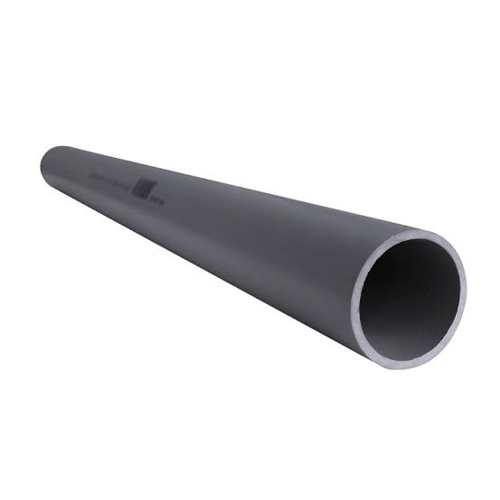
\includegraphics[height=0.5cm]{img/pvc.png} & Tour PVC de \qty{1}{m} (\qty{159}{mm} ext., \qty{144}{mm} int.) & Porte les 12 plants & 1 & \qty{1060}{XPF} & \qty{1060}{XPF} \\
\hline
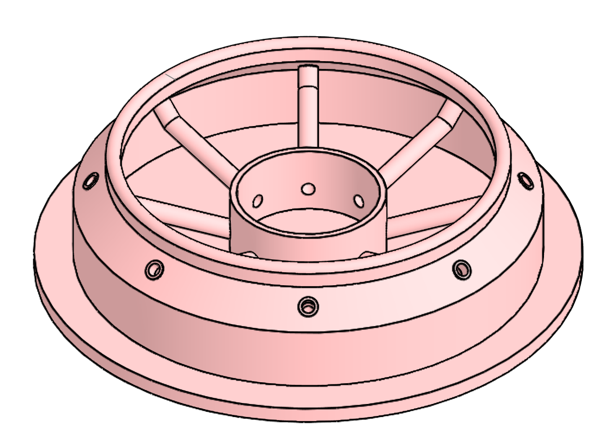
\includegraphics[height=0.5cm]{img/couvercle.png} & Couvercle répartiteur & Répartit l'eau en haut & 1 & – & – \\
\hline
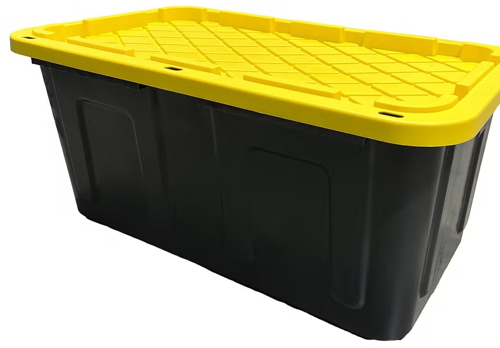
\includegraphics[height=0.5cm]{img/bac.png} & Bac de \qty{152}{L} & Réserve de solution & 1 & \qty{4160}{XPF} & \qty{4160}{XPF} \\
\hline
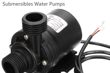
\includegraphics[height=0.5cm]{img/lpfidi.png} & Pompe de circulation \qty{12}{V} LPFIDI (Amazon) & Monte l'eau en haut & 1 & \qty{5063}{XPF} & \qty{5063}{XPF} \\
\hline
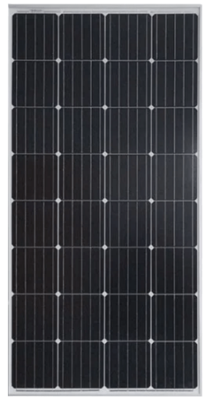
\includegraphics[height=0.5cm]{img/panneau.png} & Panneau solaire TE1250, \qty{120}{Wc} & Produit l'électricité & 1 & \qty{14320}{XPF} & \qty{14320}{XPF} \\
\hline
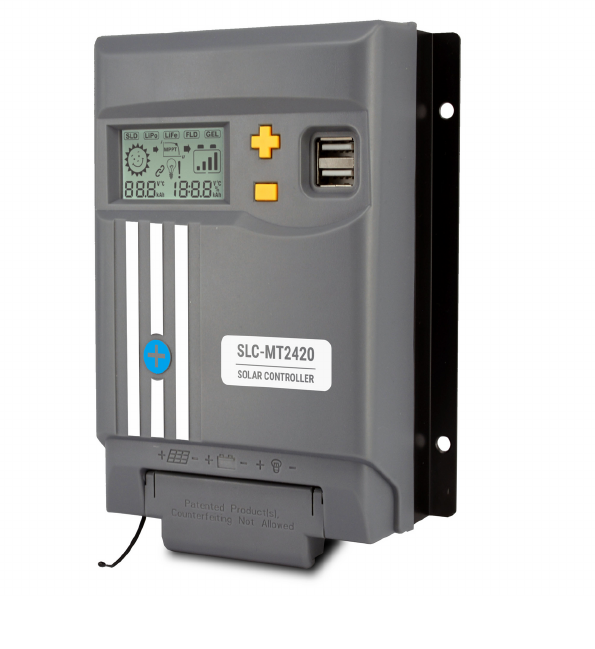
\includegraphics[height=0.5cm]{img/mppt.png} & Régulateur MPPT SLC-MT2024, \qty{20}{A} & Règle la charge & 1 & \qty{12740}{XPF} & \qty{12740}{XPF} \\
\hline
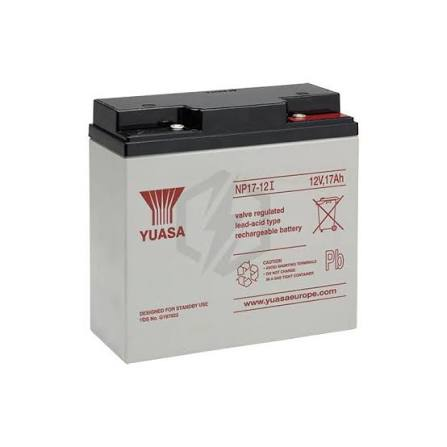
\includegraphics[height=0.5cm]{img/bat17.png} & Batterie Yuasa NP17-12I, \qty{12}{V} \qty{17}{Ah} & Stocke l'électricité & 1 & \qty{7320}{XPF} & \qty{7320}{XPF} \\
\hline
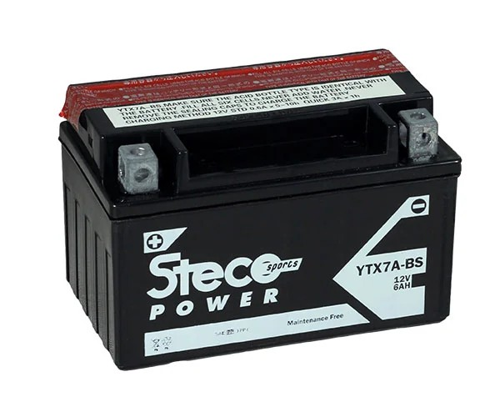
\includegraphics[height=0.5cm]{img/bat6.png} & Batterie Steco YTX7A-BS, \qty{12}{V} \qty{6}{Ah} & Stocke l'électricité & 1 & \qty{2850}{XPF} & \qty{2850}{XPF} \\
\hline
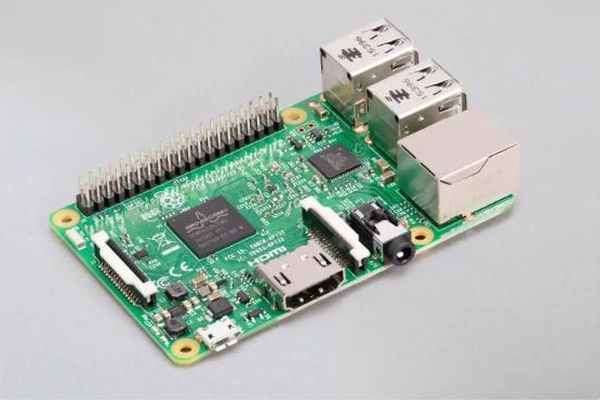
\includegraphics[height=0.5cm]{img/rpi3b.png} & Raspberry Pi 3 Model B & Le cerveau & 1 & \qty{5080}{XPF} & \qty{5080}{XPF} \\
\hline
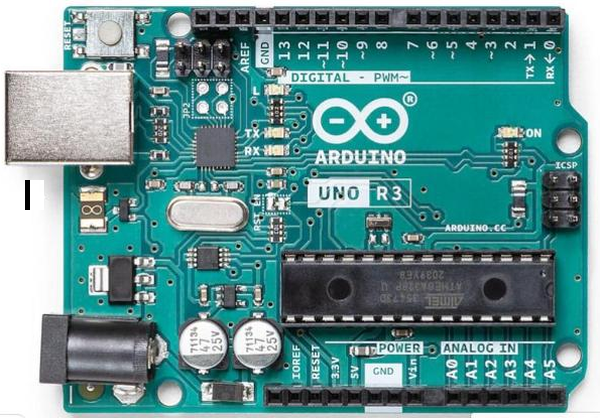
\includegraphics[height=0.5cm]{img/uno_r3.png} & Arduino Uno R3 & Exécute les ordres & 1 & \qty{2450}{XPF} & \qty{2450}{XPF} \\
\hline
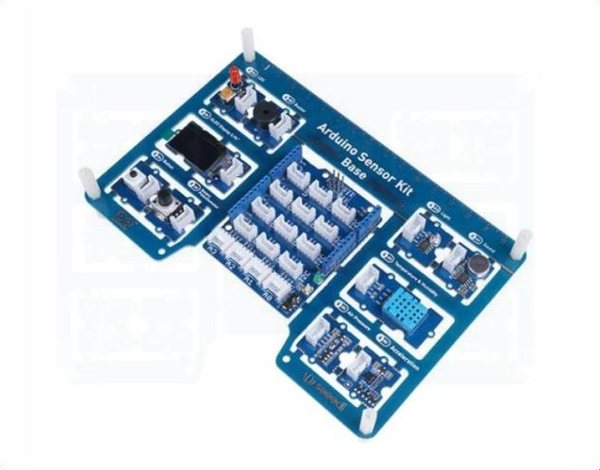
\includegraphics[height=0.5cm]{img/kit_vitta.png} & Arduino Sensor Kit (Vittascience) & Air, pression, écran, lumière & 1 & \qty{5570}{XPF} & \qty{5570}{XPF} \\
\hline
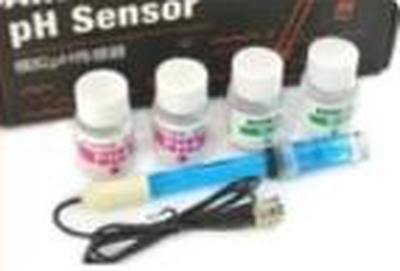
\includegraphics[height=0.5cm]{img/ph_dfrobot.png} & Sonde de pH Gravity SEN0161-V2 (DFRobot) & Mesure l'acidité & 1 & \qty{4200}{XPF} & \qty{4200}{XPF} \\
\hline
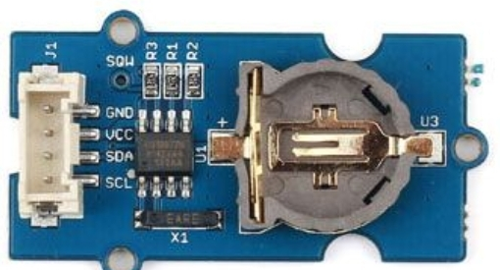
\includegraphics[height=0.5cm]{img/rtc.png} & Horloge temps réel DS1307 (Grove) & Donne l'heure & 1 & \qty{1140}{XPF} & \qty{1140}{XPF} \\
\hline
\multicolumn{6}{|c|}{\textbf{Tableau du matériel à commander pour une tour}} \\
\hline
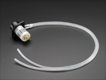
\includegraphics[height=0.5cm]{img/bom3_1.png} & Pompe péristaltique \qty{12}{V} (Adafruit) & Dosent engrais et pH & 3 & \qty{2650}{XPF} & \qty{7950}{XPF} \\
\hline
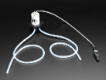
\includegraphics[height=0.5cm]{img/bom3_2.png} & Tuyau silicone d'\qty{1}{m} (Adafruit) & Tuyau de dosage & 1 & \qty{370}{XPF} & \qty{370}{XPF} \\
\hline
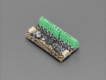
\includegraphics[height=0.5cm]{img/bom3_3.png} & Carte 8 canaux à MOSFET (Adafruit) & Commande les pompes & 1 & \qty{1590}{XPF} & \qty{1590}{XPF} \\
\hline
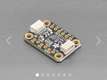
\includegraphics[height=0.5cm]{img/bom3_4.png} & Convertisseur ADS1115 (Adafruit) & Lit les sondes & 1 & \qty{1590}{XPF} & \qty{1590}{XPF} \\
\hline
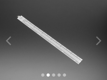
\includegraphics[height=0.5cm]{img/bom3_5.png} & Capteur de niveau eTape \qty{30}{cm} (Adafruit) & Niveau du bac & 1 & \qty{4240}{XPF} & \qty{4240}{XPF} \\
\hline
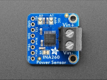
\includegraphics[height=0.5cm]{img/bom3_6.png} & Capteur INA260 (Adafruit) & Charge de la batterie & 1 & \qty{1060}{XPF} & \qty{1060}{XPF} \\
\hline
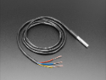
\includegraphics[height=0.5cm]{img/bom3_7.png} & Sonde de température d'eau DS18B20 (Adafruit) & Température du bac & 1 & \qty{1060}{XPF} & \qty{1060}{XPF} \\
\hline
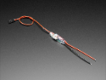
\includegraphics[height=0.5cm]{img/bom3_8.png} & Régulateur \qty{12}{V} vers \qty{5}{V} (Adafruit) & Alimente en \qty{5}{V} & 1 & \qty{1060}{XPF} & \qty{1060}{XPF} \\
\hline
\multicolumn{5}{|r|}{\textbf{Sous-total du matériel disponible}} & \textbf{\qty{65953}{XPF}} \\
\hline
\multicolumn{5}{|r|}{\textbf{Sous-total du matériel à commander}} & \textbf{\qty{18920}{XPF}} \\
\hline
\multicolumn{5}{|r|}{\textbf{Total général}} & \textbf{\qty{84873}{XPF}} \\
\hline
\end{tabularx}
\caption{Tableau du matériel de la tour : disponible et à commander.}
\end{table}


% =====================================================================
\clearpage
\partieENO{L'étude financière}

Cette partie répond à une question simple : combien coûte la tour, combien coûte son fonctionnement, et combien rapporte-t-elle ? Je commence par l'investissement de départ, repris de la partie 11. Je calcule ensuite les coûts annuels de fonctionnement, puis la valeur de la production de laitues. J'en déduis le temps de retour et le prix de revient d'une laitue. Plusieurs chiffres reposent sur des hypothèses : je les signale, parce qu'ils changeront avec les mesures et les vrais prix d'achat.

\Needspace{8\baselineskip}\subsection{L'investissement de départ}

Le matériel de la tour coûte \qty{84873}{XPF} (partie 11) : \qty{65953}{XPF} de matériel déjà disponible et \qty{18920}{XPF} à commander. S'y ajoute la livraison de la commande Adafruit par DHL Express, estimée à \qty{159,99}{USD}.

\naturecalc{calcul de coût, à partir de prix relevés et d'hypothèses ; ce n'est pas une mesure}
\begin{demonstration}[investissement total]
\resultat{I = \qty{101863}{XPF}}
Je convertis la livraison avec le taux de la partie 11 ($\qty{106,205}{XPF/USD}$) :
\begin{align*}
P_{liv} &= \qty{159,99}{USD} \times \qty{106,205}{XPF/USD}\\
P_{liv} &\approx \qty{16992}{XPF}\\
P_{liv} &\approx \qty{16990}{XPF}
\end{align*}
J'arrondis aux dix francs. L'investissement total est la somme du matériel et de la livraison :
\begin{align*}
I &= \qty{84873}{XPF} + \qty{16990}{XPF}\\
I &= \qty{101863}{XPF}
\end{align*}
La part restant à débourser est $\qty{18920}{XPF} + \qty{16990}{XPF} = \qty{35910}{XPF}$. Les taxes d'importation en Polynésie ne sont pas comprises.
\end{demonstration}

\Needspace{8\baselineskip}\subsection{Les coûts de fonctionnement}

L'électricité ne coûte rien : tout vient du panneau solaire. Les coûts sont les engrais, le correcteur de pH et le remplacement des batteries. L'eau du bac (\qty{2,3}{L/j}) est négligeable. Je ne chiffre pas les graines, la mousse de germination, les solutions d'étalonnage et le filament d'impression : leur coût est faible, mais je ne l'ai pas relevé.

\naturecalc{calcul de coût, à partir de prix relevés et d'hypothèses ; ce n'est pas une mesure}
\begin{demonstration}[coût annuel de fonctionnement]
\resultat{C_f \approx \qty{12260}{XPF/an}}
\textbf{Engrais.} La partie 5 estime à \qty{13,6}{mL/j} le volume de solution mère A, et autant de B. Sur un an :
\begin{align*}
V_{A} &= \qty{13,6}{mL/j} \times \qty{365}{j/an} = \qty{4964}{mL/an} \approx \qty{4,96}{L/an}
\end{align*}
Un lot d'engrais A et B de \qty{1}{L} chacun coûte \qty{12,90}{EUR}, soit $\qty{12,90}{EUR} \times \qty{119,332}{XPF/EUR} \approx \qty{1540}{XPF}$ (prix relevé en France, hors livraison jusqu'en Polynésie). Il faut donc $4{,}96$ lots par an :
\begin{align*}
C_{eng} &= 4{,}96 \times \qty{1540}{XPF}\\
C_{eng} &\approx \qty{7640}{XPF/an}
\end{align*}
\textbf{Correcteur de pH.} \qty{6}{mL/j}, soit $\qty{6}{mL/j} \times \qty{365}{j/an} = \qty{2190}{mL/an} = \qty{2,19}{L/an}$. Je suppose un prix de \qty{950}{XPF} le litre (hypothèse, à remplacer par le vrai prix) :
\begin{align*}
C_{pH} &= \qty{2,19}{L/an} \times \qty{950}{XPF/L} \approx \qty{2080}{XPF/an}
\end{align*}
\textbf{Batteries.} Je suppose une durée de vie de 4 ans pour les deux batteries au plomb, de prix \qty{7320}{XPF} et \qty{2850}{XPF} :
\begin{align*}
C_{bat} &= \frac{\qty{7320}{XPF} + \qty{2850}{XPF}}{4\ \text{ans}} = \frac{\qty{10170}{XPF}}{4\ \text{ans}} \approx \qty{2540}{XPF/an}
\end{align*}
Le total est la somme des trois :
\begin{align*}
C_f &= \qty{7640}{XPF/an} + \qty{2080}{XPF/an} + \qty{2540}{XPF/an}\\
C_f &= \qty{12260}{XPF/an}
\end{align*}
\end{demonstration}

\Needspace{8\baselineskip}\subsection{La valeur de la production}

La tour porte 12 laitues. Une laitue reste en tour environ 32 jours ; je compte 3 jours de nettoyage entre deux cultures, soit 35 jours par cycle. Les plants suivants sont semés en pépinière pendant que les précédents poussent, donc la tour ne reste jamais vide.

\naturecalc{calcul de coût, à partir de prix relevés et d'hypothèses ; ce n'est pas une mesure}
\begin{demonstration}[laitues par an et valeur de la production]
\resultat{R \approx \qty{47640}{XPF/an}}
Je note $n_c$ le nombre de cycles par an et $N$ le nombre de laitues par an. Un cycle dure \qty{35}{j} :
\begin{align*}
n_c &= \frac{\qty{365}{j/an}}{\qty{35}{j}} \approx 10{,}4 \qquad\text{(je retiens 10 cycles)}\\
N &= 10 \times 12 = 120\ \text{laitues/an}
\end{align*}
Le prix indicatif d'une laitue à Tahiti est d'environ \qty{397}{XPF} (valeur moyenne relevée sur internet, à confirmer au marché). La valeur de la production est :
\begin{align*}
R &= N \times p = 120 \times \qty{397}{XPF}\\
R &= \qty{47640}{XPF/an}
\end{align*}
Ce n'est pas un revenu : c'est la valeur des laitues au prix du marché, qu'elles soient vendues ou mangées. Le rendement réel sera connu à la première récolte.
\end{demonstration}

\Needspace{8\baselineskip}\subsection{Temps de retour et prix de revient}

\naturecalc{calcul de coût, à partir de prix relevés et d'hypothèses ; ce n'est pas une mesure}
\begin{demonstration}[temps de retour et prix de revient d'une laitue]
\resultat{T_r \approx \qty{2,9}{ans}\quad;\quad p_r \approx \qty{272}{XPF/laitue}}
Le gain annuel est la valeur de la production moins les coûts de fonctionnement :
\begin{align*}
G &= R - C_f = \qty{47640}{XPF/an} - \qty{12260}{XPF/an}\\
G &= \qty{35380}{XPF/an}
\end{align*}
Le temps de retour est l'investissement divisé par le gain annuel :
\begin{align*}
T_r &= \frac{I}{G} = \frac{\qty{101863}{XPF}}{\qty{35380}{XPF/an}} \approx \qty{2,9}{ans}
\end{align*}
Si l'on ne compte que ce qu'il reste à débourser (\qty{35910}{XPF}), puisque le reste du matériel est déjà acheté :
\begin{align*}
T_r' &= \frac{\qty{35910}{XPF}}{\qty{35380}{XPF/an}} \approx \qty{1,0}{an}
\end{align*}
Pour le prix de revient, j'amortis l'investissement sur 5 ans (hypothèse) :
\begin{align*}
a &= \frac{\qty{101863}{XPF}}{5\ \text{ans}} \approx \qty{20370}{XPF/an}\\
p_r &= \frac{a + C_f}{N} = \frac{\qty{20370}{XPF/an} + \qty{12260}{XPF/an}}{120\ \text{laitues/an}}\\
p_r &\approx \qty{272}{XPF/laitue}
\end{align*}
Le seuil de rentabilité est le nombre de laitues $N_s$ pour lequel la valeur égale les coûts, $N_s\,p = a + C_f$ :
\begin{align*}
N_s &= \frac{\qty{32630}{XPF/an}}{\qty{397}{XPF}} \approx 82{,}2 \longrightarrow 83\ \text{laitues/an}
\end{align*}
\end{demonstration}

\begin{aretenir}
La tour coûte \qty{101863}{XPF} (livraison comprise, hors taxes d'importation) et environ \qty{12260}{XPF} par an à faire fonctionner. Elle produit environ 120 laitues par an, d'une valeur de \qty{47640}{XPF} au prix indicatif de \qty{397}{XPF}. Le prix de revient d'une laitue est d'environ \qty{272}{XPF}, et la tour est rentable à partir de 83 laitues par an. Ces chiffres sont un temps de retour théorique estimé et un prix de revient minimal : ils ne comptent ni les graines, ni la mousse de germination, ni les solutions d'étalonnage, ni le filament d'impression, et ils supposent que les 12 emplacements sont occupés toute l'année sans perte de plants. Si les batteries vivent à \qty{35}{\celsius}, leur durée tombe vers $4 \times 0{,}42 \approx \qty{1,7}{ans}$ (partie 6.7) : le coût des batteries passe à environ \qty{6050}{XPF/an}, le coût annuel à environ \qty{15770}{XPF}, le temps de retour à environ \qty{3,2}{ans} et le prix de revient à environ \qty{300}{XPF} par laitue. L'intérêt réel de ce projet reste pédagogique : le résultat dépend du prix de vente, du rendement mesuré et de la température de l'eau (partie 6).
\end{aretenir}


% ===== PLANTES ET BILAN =====
% =====================================================================
\clearpage
\partieENO{Les plantes et les essais}

La tour n'a de sens que si elle fait pousser des plantes. Cette partie présente la plante que j'ai choisie pour commencer, la laitue, et ce que j'ai déjà observé. Je commence par les valeurs cibles de la laitue, puis par la conversion de l'EC en ppm, puis par les premiers semis avec leurs photos. Je termine par le calendrier prévu et la façon dont je suivrai la croissance.

\Needspace{8\baselineskip}\subsection{Les besoins de la laitue}

J'ai choisi la laitue pour débuter, parce qu'elle pousse vite (environ 32 jours après le repiquage) et qu'elle supporte bien l'hydroponie. Elle est cultivée en NFT (film d'eau) dans les études que j'ai trouvées, un système proche de ma tour. Le tableau donne les valeurs retenues dans le dashboard, par stade de croissance. Les jours sont comptés à partir de la mise en tour du plant.

\begin{table}[H]
\centering
\small
\begin{tabular}{|l|c|c|c|}
\hline
\textbf{Stade} & \textbf{Jours} & \textbf{EC cible (\unit{\micro S/cm})} & \textbf{pH cible} \\
\hline
Reprise & 0 à 5 & 1000 à 1200 & 5,6 à 6,0 \\
\hline
Croissance des feuilles & 5 à 22 & 1200 à 1600 & 5,6 à 6,0 \\
\hline
Pommaison & 22 à 32 & 1400 à 1800 & 5,6 à 6,0 \\
\hline
Prête à récolter & 32 et plus & 1400 à 1800 & 5,6 à 6,0 \\
\hline
\end{tabular}
\caption{Valeurs cibles de la laitue (recherche documentaire du 31 octobre 2026).}
\end{table}

Les alarmes du dashboard se déclenchent si l'EC sort de \qtyrange{800}{2200}{\micro S/cm} ou si le pH sort de 5,2 à 6,5. Au-dessus d'environ \qty{2200}{\micro S/cm}, la laitue risque des pointes de feuilles brûlées et un goût amer. L'eau idéale est entre \qty{18}{\celsius} et \qty{22}{\celsius}. La partie 6 montre que cette plage sera difficile à tenir à Tahiti : c'est un point à surveiller dès les premiers essais.

Pour la tomate cerise et le poivron, les plages sont plus élevées (EC jusqu'à \qty{2800}{\micro S/cm} pour la tomate en fructification) et leur culture est plus longue (60 à 75 jours avant la récolte). Elles sont enregistrées dans le dashboard, mais je ne les essaie qu'après la laitue.

\naturecalc{théorie (formule démontrée, valeurs de fiches techniques et hypothèses ; rien de mesuré)}
\begin{demonstration}[conversion de l'EC en ppm]
\resultat{\mathrm{ppm} = f \times EC}
Je note $EC$ la conductivité, en $\mu$S/cm, et $f$ un facteur de conversion sans unité qui dépend de l'échelle. Les appareils du commerce estiment la masse de sels dissous (en ppm, c'est-à-dire en mg/L) en multipliant la conductivité par un facteur : $f = 0{,}5$ pour l'échelle 500, $f = 0{,}7$ pour l'échelle 700. Pour la cible de croissance de la laitue, $EC = \qty{1400}{\micro S/cm}$ :
\begin{align*}
\mathrm{ppm}_{500} &= 0{,}5 \times \qty{1400}{\micro S/cm} = \qty{700}{ppm}\\
\mathrm{ppm}_{700} &= 0{,}7 \times \qty{1400}{\micro S/cm} = \qty{980}{ppm}
\end{align*}
La conversion dépend de l'échelle : je donne donc toujours l'EC en $\mu$S/cm, qui est la grandeur mesurée.
\end{demonstration}

\Needspace{8\baselineskip}\subsection{Les premiers semis}

J'ai semé les premières laitues le \qty{27}{octobre}. Elles poussent, sans eau nutritive pour l'instant, sous la seule lumière d'une fenêtre. Elles mesuraient environ \qty{5}{cm} le 11 novembre, soit 15 jours après le semis. Les photos montrent les plants dans la mousse de germination.

\begin{figure}[H]
\centering
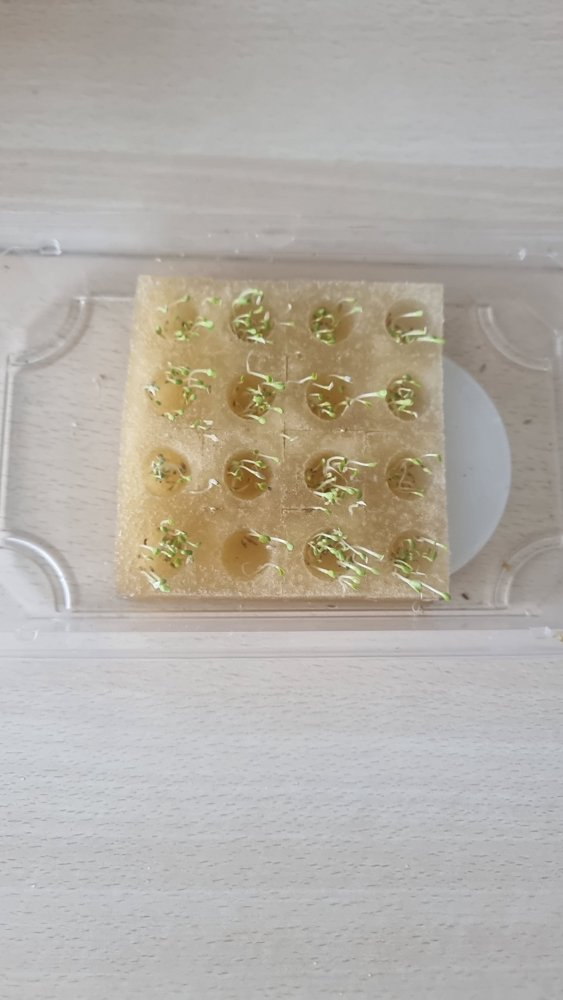
\includegraphics[height=6.2cm]{img/germ_haut2.jpg}\hfill
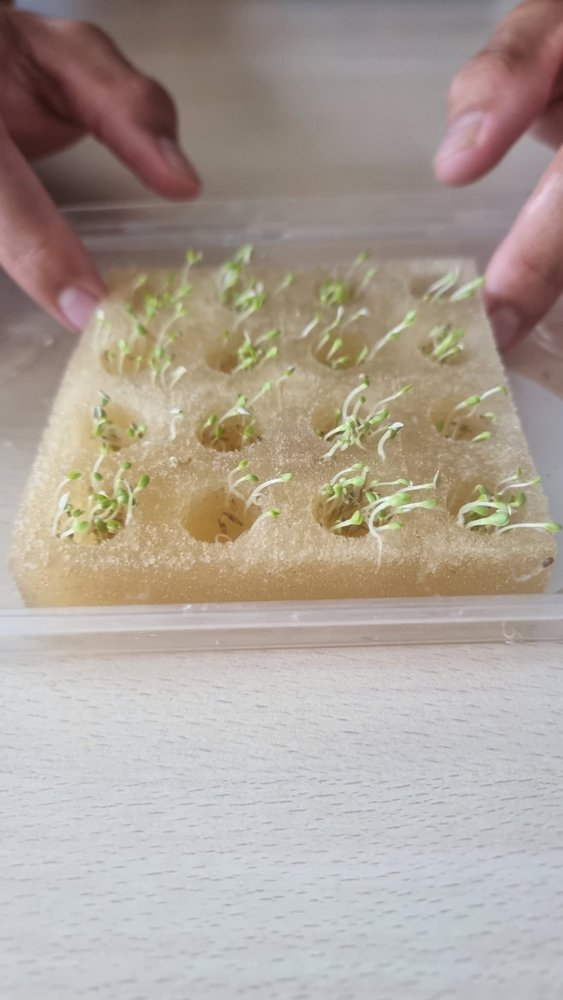
\includegraphics[height=6.2cm]{img/germ_main.jpg}\hfill
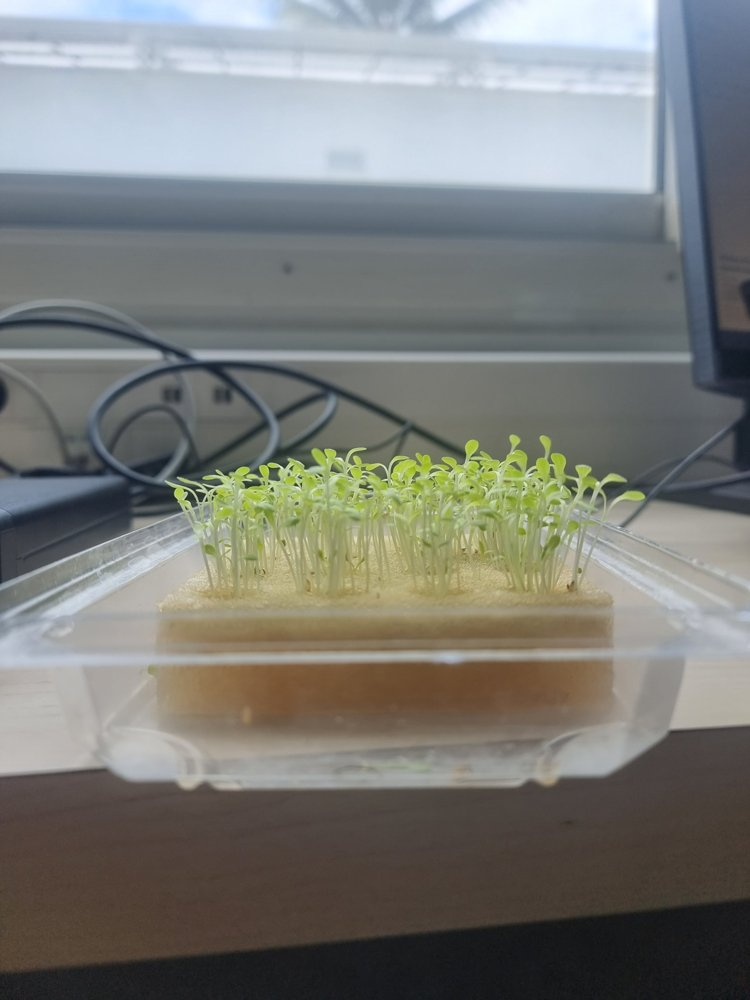
\includegraphics[height=6.2cm]{img/germ_cote.jpg}
\caption{Les semis de laitue dans la mousse de germination : vue de dessus, plants tenus à la main, vue de côté.}
\end{figure}

\Needspace{8\baselineskip}\subsection{Le calendrier prévu et le suivi}

D'après la recherche documentaire, le passage du semis au repiquage dure environ 18 jours pour la laitue, et la pleine maturité arrive vers le jour 32 après la mise en tour.

\naturecalc{prévision, à partir de la date de semis observée (27 octobre) et de durées tirées de la littérature}
\begin{demonstration}[dates prévues]
\resultat{\text{récolte} \approx 16\ \text{décembre 2026}}
Je note $d_s$ la date du semis, $d_r$ celle de la mise en tour et $d_h$ celle de la récolte. Le repiquage a lieu 18 jours après le semis, la récolte 32 jours après le repiquage :
\begin{align*}
d_r &= d_s + \qty{18}{j} = \text{27 octobre} + \qty{18}{j}\\
d_r &= \text{14 novembre}
\end{align*}
\begin{align*}
d_h &= d_r + \qty{32}{j} = \text{14 novembre} + \qty{32}{j}
\end{align*}
Du 14 au 30 novembre, il y a 16 jours ; il en reste $32 - 16 = 16$ en décembre :
\begin{align*}
d_h &= \text{16 décembre 2026}
\end{align*}
La fourchette de la littérature (25 à 45 jours après le repiquage) donne une récolte entre le 9 décembre 2026 et le 29 décembre 2026.
\end{demonstration}

Pour le suivi, je compterai chaque semaine le nombre de plants vivants, je mesurerai la hauteur de trois plants repères avec une règle et je photographierai la tour du même endroit. Je noterai aussi la date de passage à l'eau nutritive, la température de l'eau et les corrections de dosage faites par le Pi. À la récolte, je pèserai les 12 laitues pour connaître le rendement réel, que j'utilise dans l'étude financière.

\begin{aretenir}
La laitue demande un pH de 5,6 à 6,0 et une EC de 1200 à \qty{1600}{\micro S/cm} en croissance. Les premières sont semées depuis le 27 octobre et mesurent environ \qty{5}{cm} au 11 novembre. La récolte est attendue vers le 16 décembre, sous réserve du passage à l'eau nutritive et de la température de l'eau.
\end{aretenir}


% =====================================================================
\clearpage
\partieENO{Le bilan}

Cette dernière partie fait le point sur le projet. Je commence par le montage réalisé le 12 novembre 2026 à l'UPF, avec des photos de la tour et de l'installation solaire. Je présente ensuite le tableau d'avancement de chaque fonction, avec ce qui est calculé, ce qui est vérifié sur du vrai matériel et ce qui reste à faire. Je liste ensuite les points ouverts, c'est-à-dire les hypothèses à remplacer par des mesures. Je termine par les prochaines étapes.

\subsection{Le montage réalisé à l'UPF}

Le 12 novembre 2026, nous avons monté la tour à l'UPF, mon coéquipier Gabriel Piritua et moi, ensemble. Le montage de l'installation est le fruit du travail de Gabriel : c'est lui qui a conçu et réalisé la structure métallique qui porte le panneau solaire et le plateau de l'armoire électrique. Nous avons monté ensemble le panneau solaire et la batterie sur cette structure, puis installé la tour sur son bac, devant elle, sur la coursive extérieure du bâtiment. Le régulateur solaire est en place dans l'armoire et son écran est allumé. Avant de brancher le panneau, il indiquait \qty{13,2}{V}, la tension de la batterie seule. Une fois le panneau branché, cette tension a monté avec l'ensoleillement, ce qui montre que le panneau charge bien la batterie.

\begin{figure}[H]
\centering
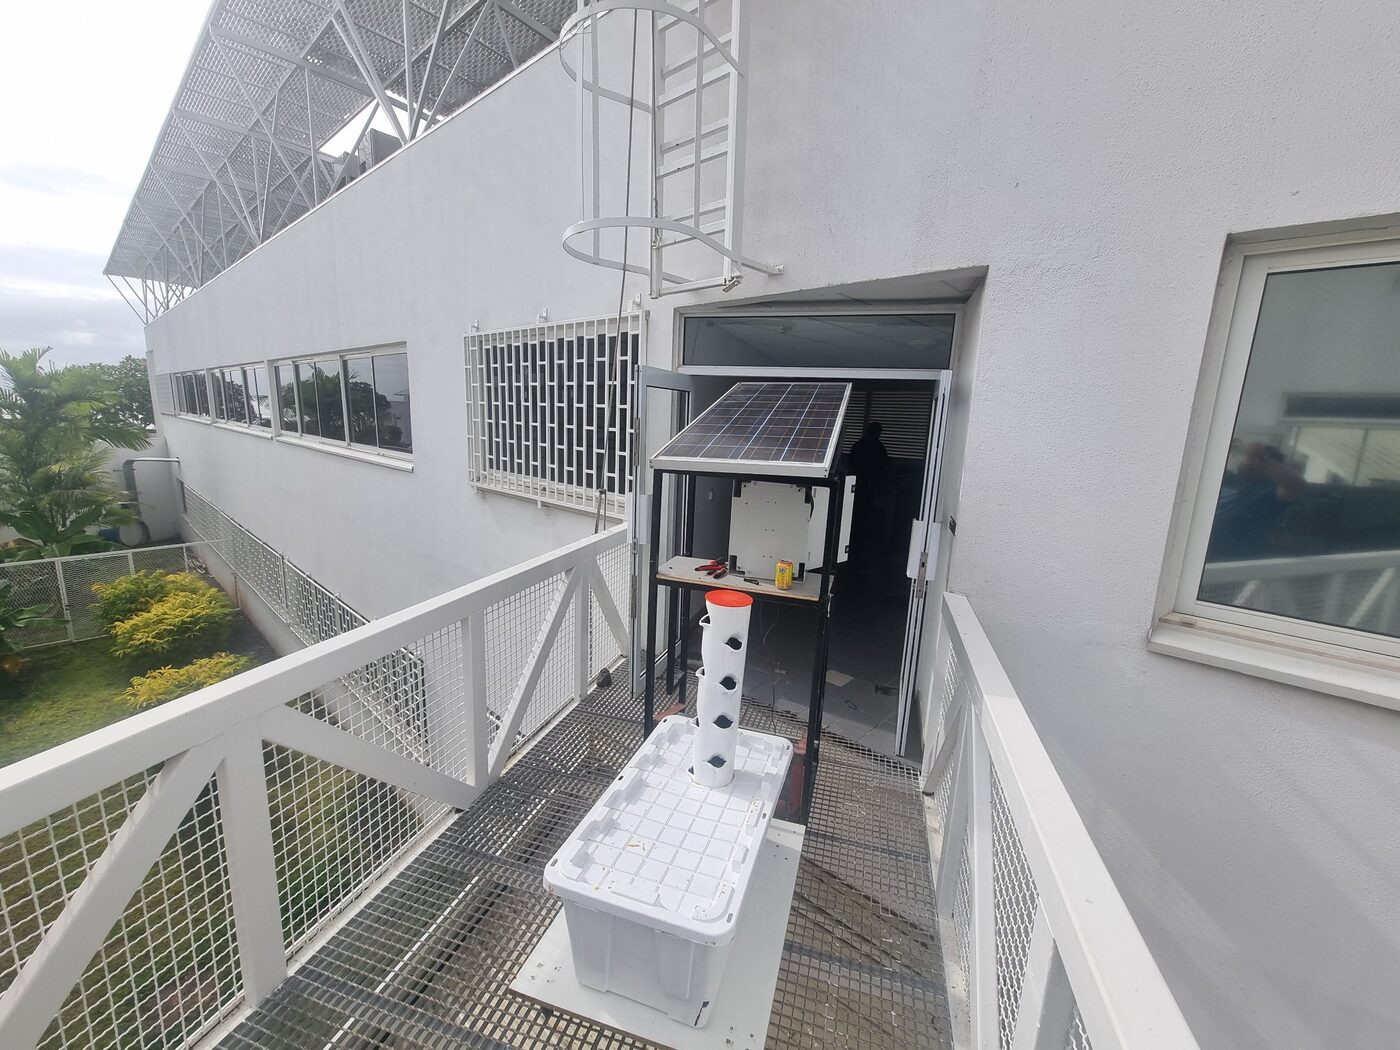
\includegraphics[width=0.9\linewidth]{img/montage/ensemble.jpg}
\caption{Vue d'ensemble : la tour et son bac au premier plan, la structure qui porte le panneau solaire et le plateau de l'armoire derrière.}
\end{figure}

\begin{figure}[H]
\centering
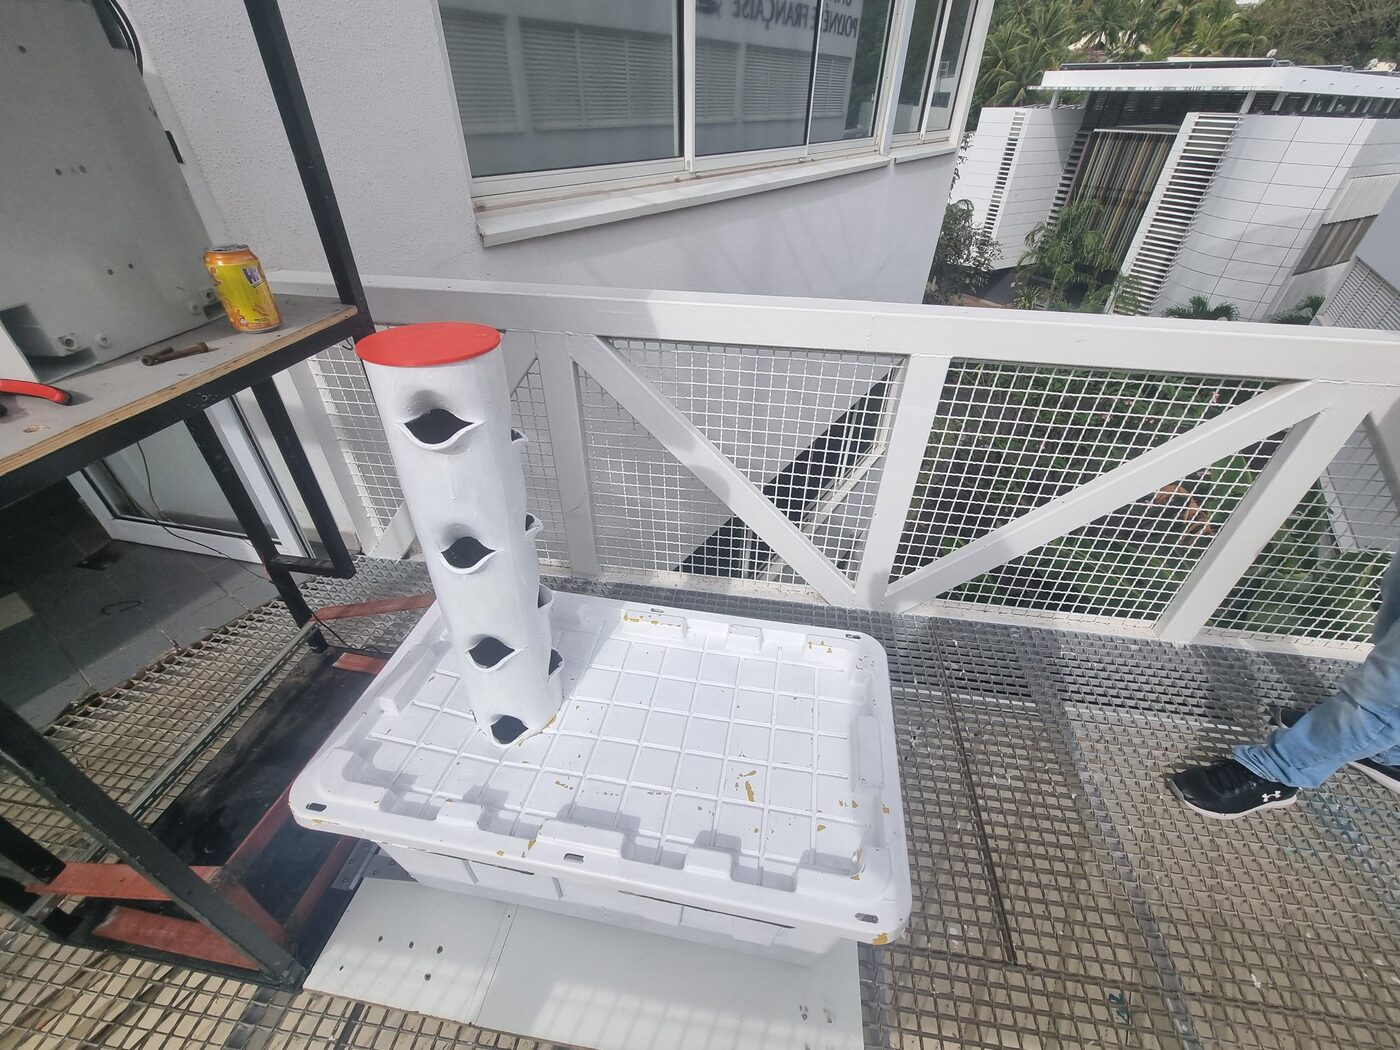
\includegraphics[width=0.78\linewidth]{img/montage/tour.jpg}
\caption{La tour posée sur le couvercle du bac, avec ses trous de plantation.}
\end{figure}

\begin{figure}[H]
\centering
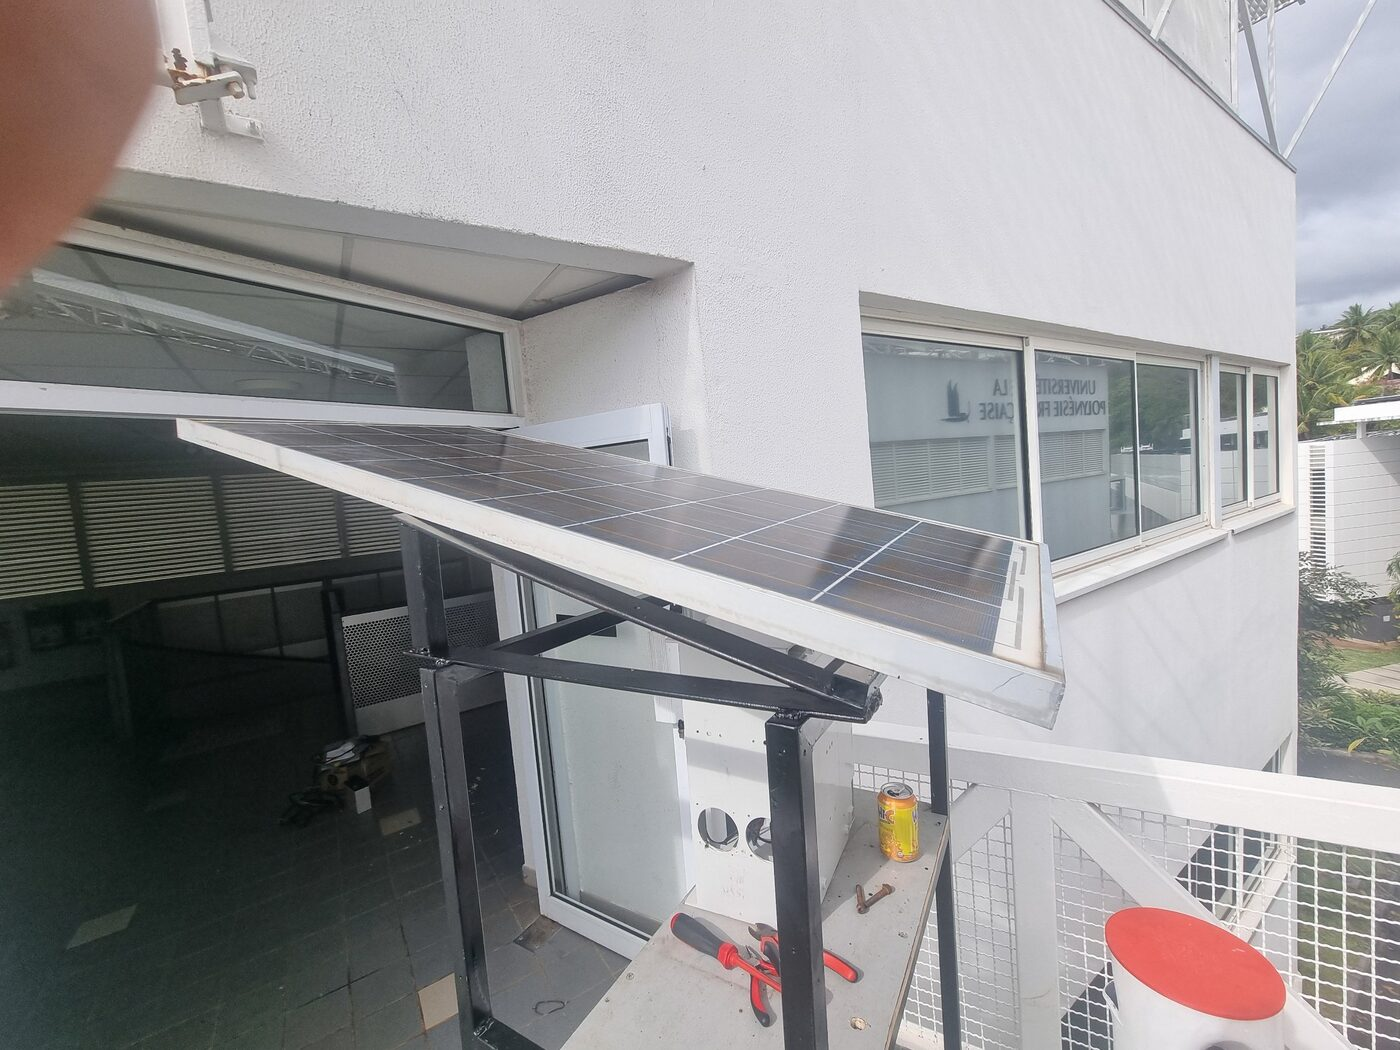
\includegraphics[width=0.9\linewidth]{img/montage/panneau.jpg}
\caption{Le panneau solaire, incliné, sur la structure métallique soudée.}
\end{figure}

\begin{figure}[H]
\centering
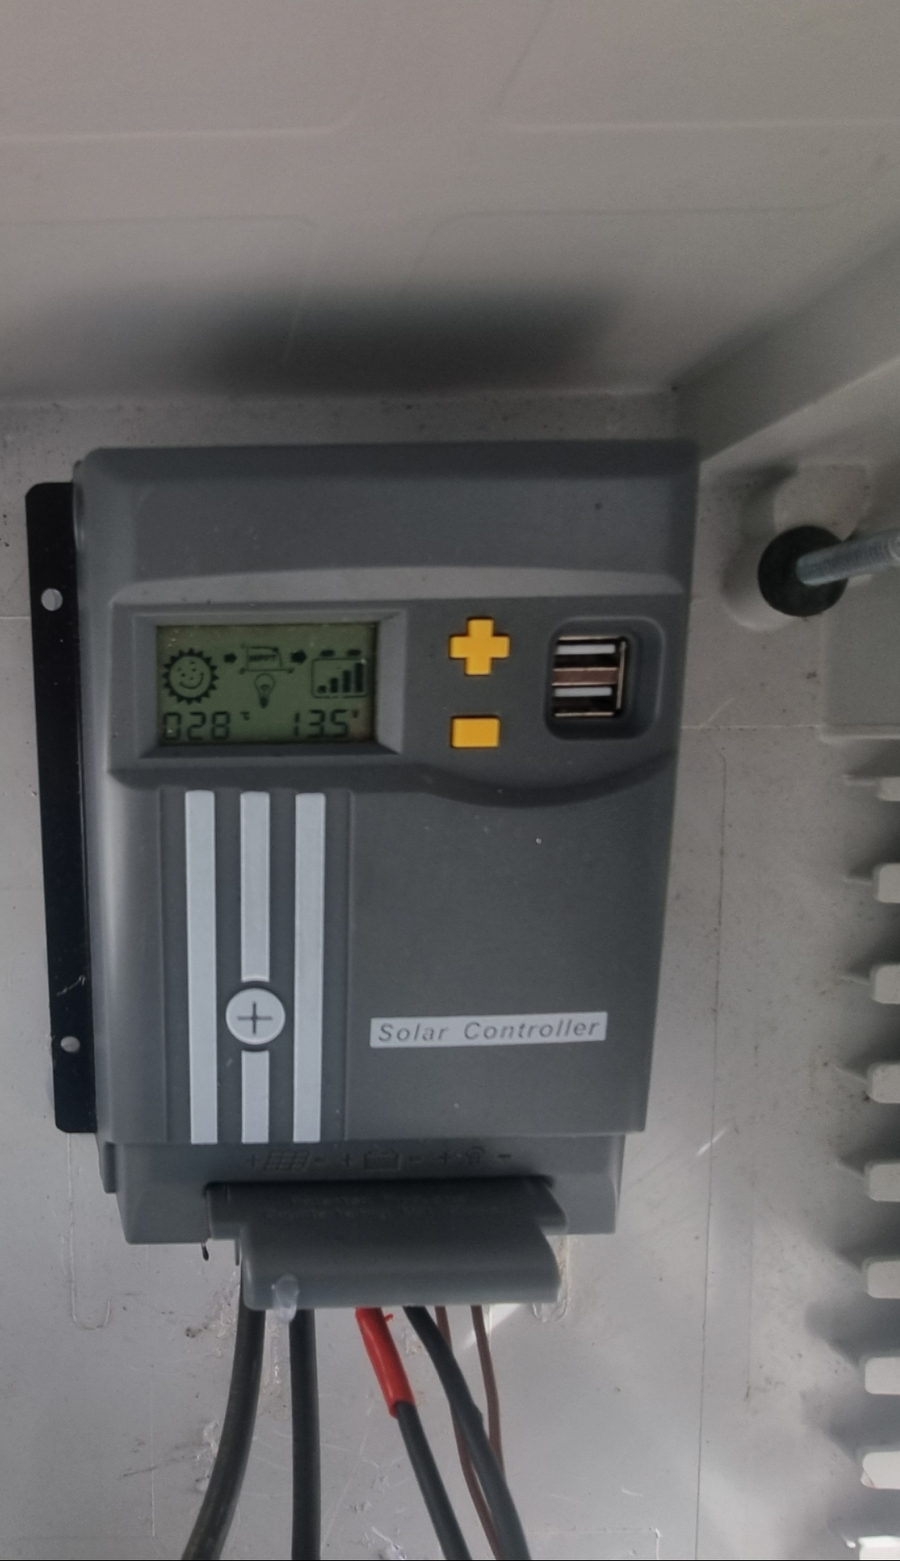
\includegraphics[height=0.32\textheight]{img/montage/regulateur.jpg}
\caption{Le régulateur solaire dans l'armoire, écran allumé (\qty{13,5}{V} au moment de la photo).}
\end{figure}

\textbf{Ce qui reste à faire sur le montage.} Il reste à fixer l'armoire électrique sur le plateau : c'est la suite du travail de Gabriel. De mon côté, je dois modéliser et imprimer le support qui tient la tour dans le bac, puis mesurer le débit réel de la pompe et les pertes de charge réelles du circuit, pour remplacer les valeurs calculées des parties 3 et 4 par des mesures.

\Needspace{8\baselineskip}\subsection{L'état d'avancement}

Le tableau suivant donne l'état d'avancement de chaque fonction de la tour.

\begin{table}[H]
\centering
\scriptsize
\renewcommand{\arraystretch}{1.1}
\begin{tabularx}{\textwidth}{|>{\raggedright\arraybackslash}p{2.6cm}|Y|Y|Y|}
\hline
\textbf{Fonction} & \textbf{Ce qui est fait} & \textbf{Ce qui est vérifié} & \textbf{Ce qui reste} \\
\hline
Circuit d'eau & Débit calculé : \qty{388}{L/h}, \qty{32}{L/h} par plant ; couvercle conçu et imprimé en 3D & Rien mesuré & Mesurer le débit réel, la répartition, la consommation d'eau \\
\hline
Mécanique & Masse du tube, trous, stabilité au vent calculés & Rien mesuré & Peser et mesurer le bac ; lester si bac presque vide \\
\hline
Énergie solaire & Consommation \qty{227}{Wh/j}, production \qty{272}{Wh/j} en juin, batteries, câbles, fusibles calculés & Le 12 novembre : batterie à \qty{13,2}{V}, et le panneau la charge ; rien d'autre mesuré & Lire l'étiquette de la Steco ; mesures M1 à M5 ; limiter le courant de charge \\
\hline
Thermodynamique & Bilan de chaleur du bac, effet du bac blanc, chaleur de la pompe & Rien mesuré & Enregistrer 24 h la température de l'eau et de l'air ; chercher une solution de refroidissement \\
\hline
Sonde EC & Principe, constante $K$ estimée entre \qty{0,97}{cm^{-1}} et \qty{3,04}{cm^{-1}}, formules et schéma & Montée et mesurée dans l'eau le 20 novembre 2026 : \qty{1438}{\micro S\per cm} avec l'étalonnage de départ (partie 9.4) & Étalonner avec deux solutions, en déduire $P$ et $K$ \\
\hline
Sonde de pH & Étalonnage en deux points, formules & Vérifiée le 1\textsuperscript{er} novembre (près d'une demi-heure de mesures) & Étalonner régulièrement ; suivre la dérive \\
\hline
Arduino & ConfigurableFirmata (flash \qty{39,9}{\percent}), coupure des pompes après \qty{30}{s} de silence & Tourne sur la carte depuis le 1\textsuperscript{er} novembre : lecture du pH, de l'air et de l'heure & Essai avec la carte MOSFET\ix{15} et les pompes ; protection locale du niveau à ajouter \\
\hline
Raspberry Pi & Programme de pilotage (\texttt{pilote.py}), serveur, dashboard, accès à distance & Chaîne de mesure vérifiée le 1\textsuperscript{er} novembre ; pilotage testé avec un Arduino simulé & Essai du pilotage sur les vraies pompes, planning de jour et de nuit compris \\
\hline
Plantes & Semis le 27 octobre & Laitues d'environ \qty{5}{cm} au 11 novembre & Repiquage vers le 14 novembre, passage à l'eau nutritive, récolte vers le 16 décembre \\
\hline
Finances & Investissement \qty{101863}{XPF}, coût annuel \qty{12260}{XPF}, retour \qty{2,9}{ans} & Prix indicatifs à confirmer & Relever les vrais prix (engrais, correcteur de pH, laitue au marché) \\
\hline
\end{tabularx}
\caption{État d'avancement de chaque fonction de la tour.}
\end{table}

\Needspace{8\baselineskip}\subsection{Les points ouverts}

Plusieurs hypothèses de ce rapport doivent être remplacées par des mesures. Le régulateur est un SLC-MT2024 alors que l'étude électrique de départ prévoyait un autre modèle (SLC-MPPT2420D) : j'ai recalculé avec la fiche du SLC-MT2024, mais le courant de charge réglable reste à lire dans sa notice. La technologie de la batterie Steco est à lire sur son étiquette, car je l'ai supposée de type AGM comme la Yuasa. Le prix du tube de PVC est un prix équivalent pour un diamètre de \qty{160}{mm}. Les dimensions du bac, les masses, le coefficient d'échange thermique, le débit des doseuses et la hauteur du tuyau de montée sont des hypothèses. Pour la protection de la pompe contre la marche à sec, l'Arduino actuel ne lit pas le niveau d'eau : cette fonction est à ajouter ou à confirmer. Pour la sonde EC, la sonde est maintenant montée et mesure, mais la constante de cellule reste inconnue tant que l'étalonnage à deux solutions n'est pas fait : la valeur affichée aujourd'hui repose sur la constante estimée. Enfin, le tuyau de la tour (flexible de \qty{9}{mm}) limite le débit : il faut mesurer le débit réel.

Un point reste important pour les plantes : d'après le bilan thermique complet (partie 6), l'eau du bac sera vers \qtyrange{26}{27}{\celsius} avec un air à \qty{27}{\celsius} (le premier calcul, plus simple, donnait \qty{28}{\celsius}), au-dessus de la plage idéale de la laitue. C'est un scénario calculé qui repose sur des hypothèses non mesurées (part de la chaleur d'évaporation prélevée dans l'eau, ciel dégagé la moitié du temps) et que l'enregistrement de 24 h doit confirmer. C'est le premier problème que les essais devront résoudre.

\Needspace{8\baselineskip}\subsection{Les prochaines étapes}

D'abord, je modélise et j'imprime le support de la tour dans le bac, puis je mesure le débit réel de la pompe et les pertes de charge réelles. Je repique ensuite les laitues dans la tour vers le 14 novembre, avec de l'eau seule, pour mesurer le débit et la répartition. Ensuite, je passe à l'eau nutritive en suivant le pH et l'EC à la main. La sonde EC étant désormais montée et en service, il me reste à l'étalonner avec les deux solutions. Une fois ces mesures faites, je branche l'Arduino aux pompes pour les premiers essais du pilotage automatique, avec la circulation d'abord, puis les doseuses. Enfin, je remplace les hypothèses par les mesures et je mets à jour ce rapport.

\begin{aretenir}
Le projet est abouti sur le papier : chaque fonction est dimensionnée et démontrée. Il lui manque surtout des mesures sur le vrai matériel. Les trois priorités sont : mesurer la température de l'eau, vérifier la batterie Steco avant de relier les deux batteries, et essayer le programme de l'Arduino sur les pompes.
\end{aretenir}


% ===== ANNEXES ET BIBLIOGRAPHIE =====
% ===== ANNEXES (numérotées) =====
\annexepaysage[page=1,trim=700bp 30bp 30bp 80bp,clip]{Plan_couvercle_repartiteur.pdf}{Plan du couvercle répartiteur}{planrep}{Plan du couvercle répartiteur : vue de dessus, vue de côté, vue de dessous avec les huit canaux et coupe B-B. Il est présenté dans la partie 3.2.}
\hypertarget{planrep}{}
\annexepaysage[page=1]{Plan_couvercle_bouchon.pdf}{Plan de la pièce COUVERCLE (bouchon et embout)}{planbou}{Plan de la pièce COUVERCLE (bouchon et embout). Il est présenté dans la partie 3.2.}
\hypertarget{planbou}{}
\annexepaysage{Schema_hydraulique_hydroponie.pdf}{Schéma hydraulique de la tour}{hydro}{Schéma hydraulique de la tour : bac unique, pompe de circulation -M1, pompes de dosage -M2 à -M4, sondes -B1 à -B4 et appoint manuel. Il est présenté dans la partie 3.1.}

\clearpage\refstepcounter{annexe}\phantomsection\addcontentsline{toc}{section}{Annexe \theannexe{} : Fiche du régulateur MPPT\ix{19} SLC-MT2024}
{\thispagestyle{empty}\centering{\large\bfseries Annexe \theannexe{} : Fiche du régulateur MPPT\ix{19} SLC-MT2024\par}\vspace{4pt}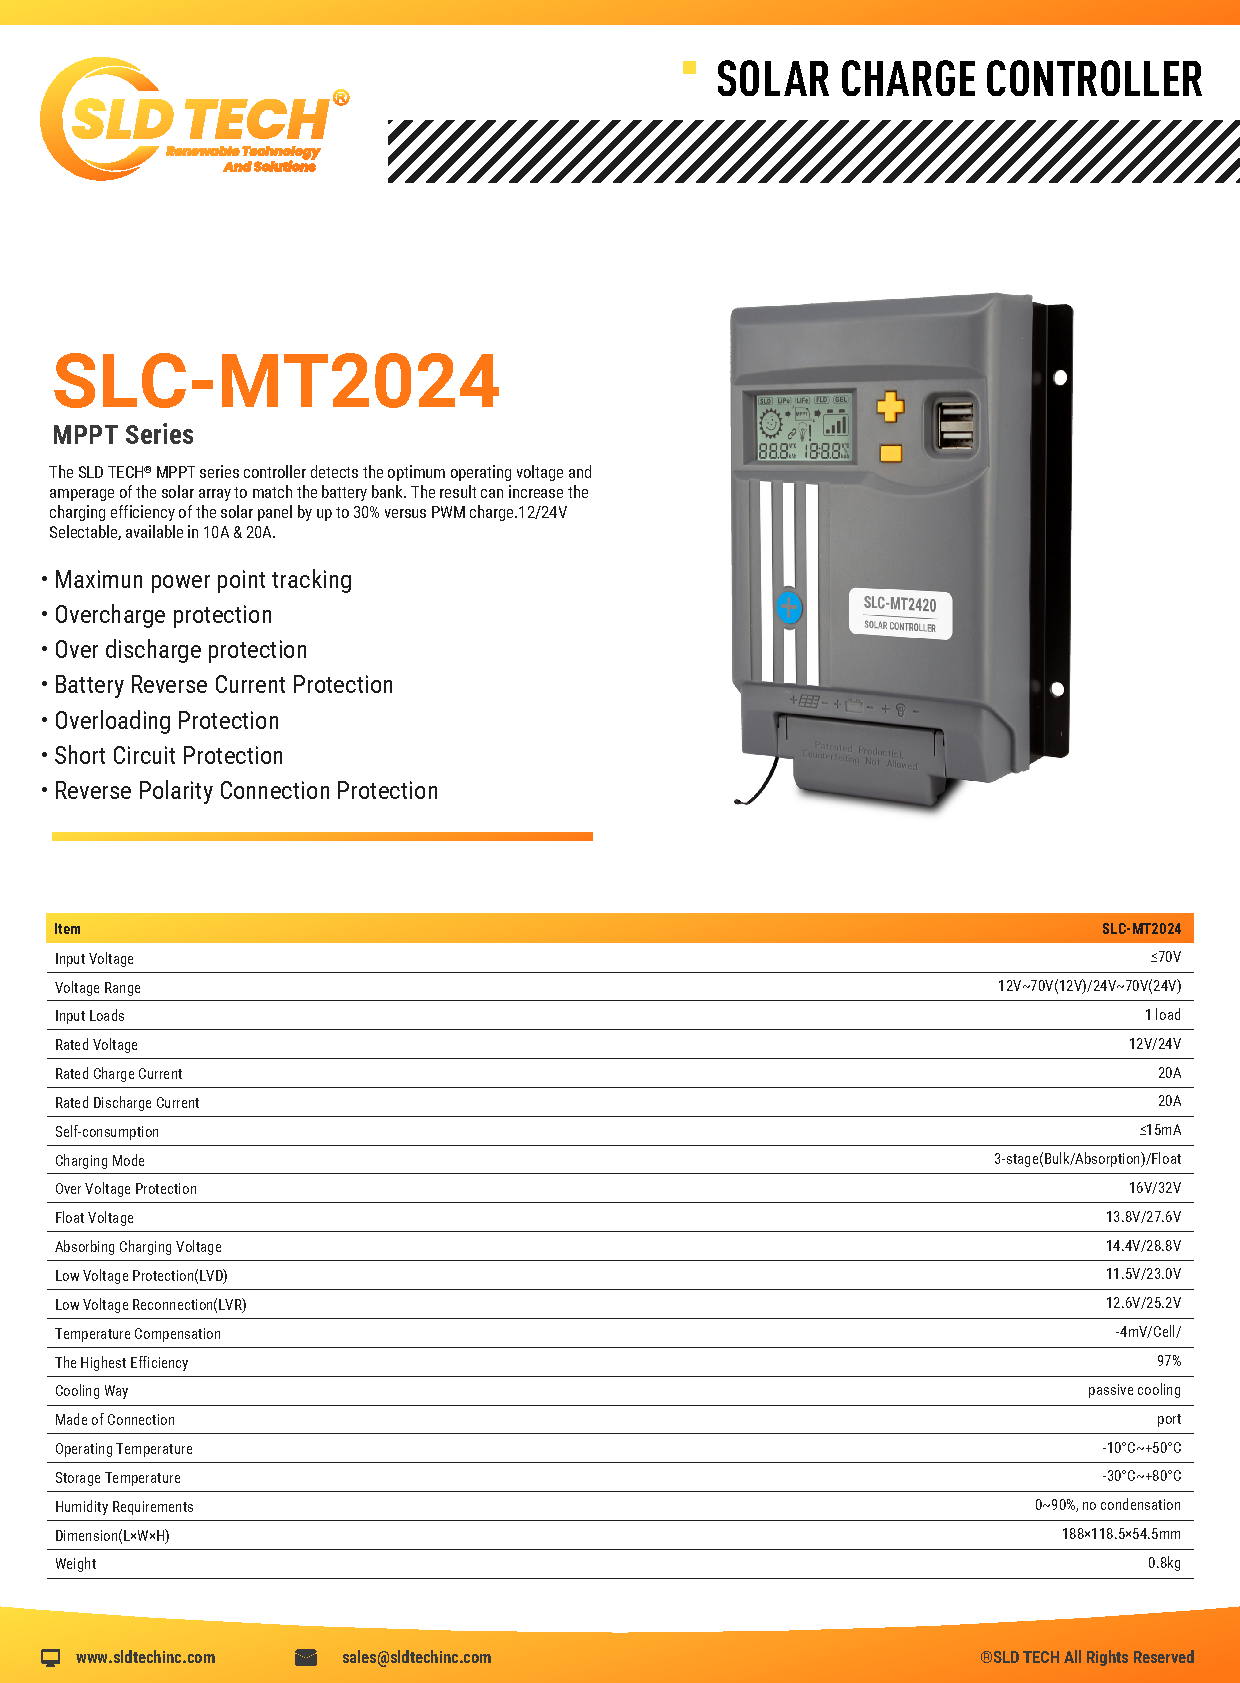
\includegraphics[page=1,width=\textwidth,height=0.86\textheight,keepaspectratio]{SLC-MT2024.pdf}\par}
\clearpage
{\begin{landscape}\thispagestyle{empty}\centering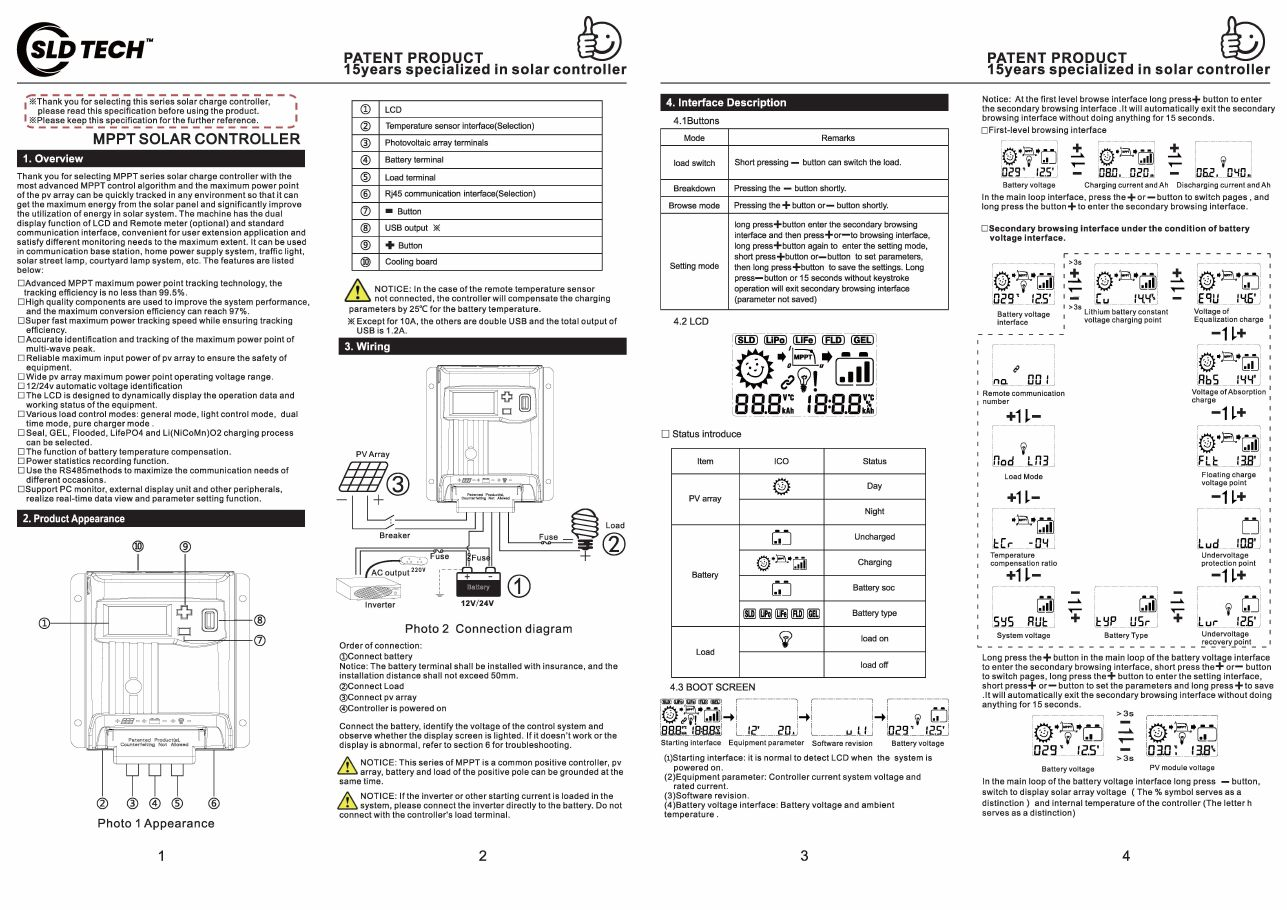
\includegraphics[height=0.93\textwidth,width=0.97\linewidth,keepaspectratio]{img/mppt_manuel_1.jpg}\end{landscape}}
\clearpage
{\begin{landscape}\thispagestyle{empty}\centering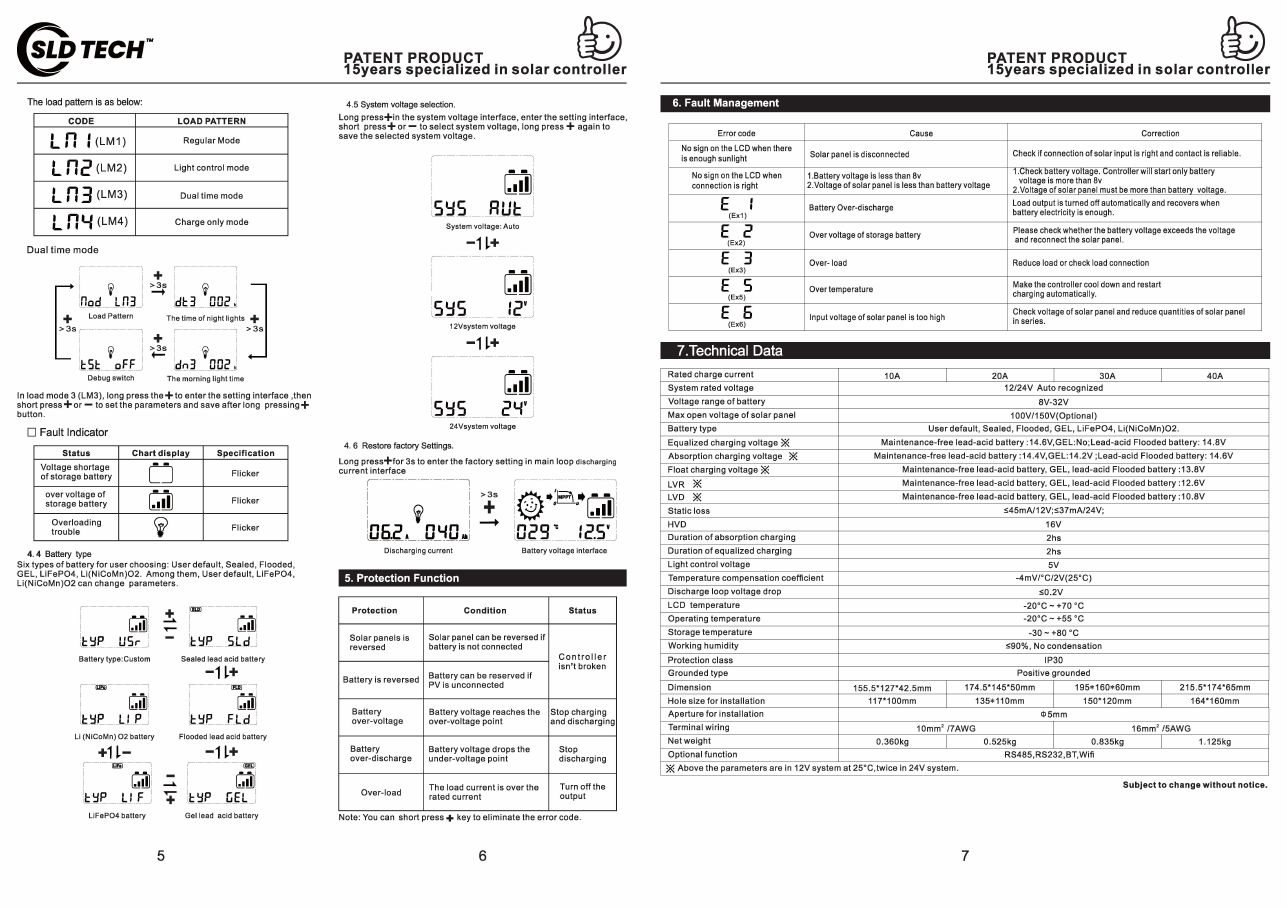
\includegraphics[height=0.93\textwidth,width=0.97\linewidth,keepaspectratio]{img/mppt_manuel_2.jpg}\end{landscape}}

\annexepaysage[page=1]{A000066-schematics.pdf}{Schéma électrique de l'Arduino Uno}{uno1}{Schéma électrique officiel de la carte Arduino Uno Rev3 (référence A000066), publié par le constructeur : alimentation, microcontrôleur et liaison USB. Les noms des broches (D5, D6, A0, A4, A5...) servent de repère pour lire les feuilles de commande de la partie 8.2.}
\pagesuite[page=2]{A000066-schematics.pdf}{uno2}{Schéma électrique officiel de la carte Arduino Uno Rev3 (suite) : les connecteurs.}

% ============================================================
\clearpage
\section*{Fiches techniques du matériel}
\addcontentsline{toc}{section}{Fiches techniques du matériel}

Chaque composant a sa fiche, qui est une annexe numérotée. Elles rassemblent, composant par composant, les caractéristiques utiles à la tour : celles des fiches techniques des fabricants et celles que j'ai relevées sur les pages des revendeurs. Pour chaque composant, je rappelle ensuite ce que la valeur change dans le projet. Les composants sont classés dans l'ordre du tableau de la partie 11 : structure et hydraulique, énergie, calcul et commande, mesures. Une valeur marquée « à mesurer » n'est pas une donnée du fabricant : c'est une hypothèse de mes calculs, à vérifier sur le montage réel.

\Needspace{8\baselineskip}
\subsection*{Structure et hydraulique}

\annexefiche{Tube PVC et bac}
\noindent Le tube est un tube de \qty{1}{m} de diamètre extérieur \qty{159}{mm} et de diamètre intérieur \qty{144}{mm}, dont l'épaisseur de paroi vaut donc :
\[
e = \frac{\qty{159}{mm} - \qty{144}{mm}}{2} = \qty{7,5}{mm}
\]
Le bac fait \qty{152}{L}. Les dimensions du bac et les masses sont des hypothèses de la partie 4, à mesurer.

\annexefiche{Pompe de circulation LPFIDI}
\noindent
\begin{table}[H]
\centering
\begin{tabularx}{\linewidth}{lY}
\hline
Caractéristique & Valeur \\
\hline
Tension d'alimentation & \qty{12}{V} continu \\
Puissance & \qty{19}{W} \\
Courant maximal & \qty{1}{A} \\
Débit maximal & \qty{800}{L/h} \\
Hauteur manométrique maximale & \qty{5}{m} \\
Sortie & filetage mâle 1/2 pouce \\
Câble & très court (rallonge à prévoir) \\
\hline
\end{tabularx}
\end{table}
Le point de fonctionnement réel de la tour est de \qty{388}{L/h} pour une hauteur de \qty{2,57}{m} (partie 3) : la pompe travaille donc bien en dessous de son débit maximal.

\Needspace{8\baselineskip}
\subsection*{Énergie}

\annexefiche{Panneau TE1250 (120 W crête)}
\noindent
\begin{table}[H]
\centering
\begin{tabularx}{\linewidth}{lY}
\hline
Caractéristique & Valeur \\
\hline
Puissance crête $P_c$ & \qty{120}{W} \\
Puissance minimale & \qty{117,5}{W} \\
Tension au point de puissance max $V_{mp}$ & \qty{17,6}{V} \\
Courant au point de puissance max $I_{mp}$ & \qty{6,8}{A} \\
Courant de court-circuit $I_{sc}$ & \qty{7,3}{A} \\
Tension à vide $V_{oc}$ & \qty{22,0}{V} \\
Fusible série maximal & \qty{10}{A} \\
NOCT & \qty{47}{\celsius} \\
\hline
\end{tabularx}
\end{table}
Les coefficients de température que j'utilise (tension $-\qty{80}{mV/\celsius}$, courant $+\qty{0,065}{\percent/\celsius}$, puissance $-\qty{0,5}{\percent/\celsius}$) sont ceux d'un panneau voisin : ce sont des hypothèses. Vérification de la cohérence de la puissance crête :
\begin{align*}
P_{mp} &= V_{mp} \times I_{mp}\\
P_{mp} &= \qty{17,6}{V} \times \qty{6,8}{A}\\
P_{mp} &= \qty{119,68}{W} \approx \qty{120}{W}
\end{align*}

\annexefiche{Régulateur MPPT SLC-MT2024}
\noindent
\begin{table}[H]
\centering
\begin{tabularx}{\linewidth}{lY}
\hline
Caractéristique & Valeur \\
\hline
Tension nominale batterie & \qty{12}{V} ou \qty{24}{V} (détection) \\
Tension d'entrée maximale & \qty{70}{V} \\
Courant de charge / de décharge & \qty{20}{A} / \qty{20}{A} \\
Sortie charge & 1 \\
Autoconsommation & $\leq \qty{15}{mA}$ \\
Charge & 3 étages \\
Absorption / floating & \qty{14,4}{V} / \qty{13,8}{V} \\
Coupure basse (LVD) / reconnexion (LVR) & \qty{11,5}{V} / \qty{12,6}{V} \\
Compensation en température & $-\qty{4}{mV}$ par élément \\
Rendement maximal & \qty{97}{\percent} \\
Refroidissement & passif \\
Température de service & \qtyrange{-10}{50}{\celsius} \\
Dimensions & \qtyproduct{188 x 118,5 x 54,5}{mm} \\
Masse & \qty{0,8}{kg} \\
\hline
\end{tabularx}
\end{table}
La coupure basse à \qty{11,5}{V} protège la batterie plomb d'une décharge profonde ; je m'en sers dans le bilan d'autonomie.

\annexefiche{Batteries au plomb}
\noindent
\begin{table}[H]
\centering
\begin{tabularx}{\linewidth}{lYY}
\hline
Caractéristique & Yuasa NP17-12I & Steco YTX7A-BS \\
\hline
Technologie & plomb étanche à soupape (VRLA, AGM) & sans entretien (AGM supposée) \\
Tension nominale & \qty{12}{V} & \qty{12}{V} \\
Capacité & \qty{17}{Ah} (20 h, jusqu'à \qty{10,5}{V}) & \qty{6}{Ah} \\
Capacité à 10 h & \qty{15,7}{Ah} (jusqu'à \qty{10,8}{V}) & non relevée \\
Dimensions (L x l x h) & \qtyproduct{181 x 76 x 167}{mm} & à relever sur l'étiquette \\
Masse & \qty{6,1}{kg} & à relever \\
Bornes & M5 femelles & à relever \\
Température de service & \qtyrange{-15}{50}{\celsius} (revendeur) & non relevée \\
\hline
\end{tabularx}
\end{table}
Le courant de décharge sur 20 h de la Yuasa se déduit de sa capacité :
\begin{align*}
I_{20} &= \frac{C_{20}}{t}\\
I_{20} &= \frac{\qty{17}{Ah}}{\qty{20}{h}}\\
I_{20} &= \qty{0,85}{A}
\end{align*}
L'énergie nominale des deux batteries mises en parallèle vaut :
\begin{align*}
E &= U \times (C_1 + C_2)\\
E &= \qty{12}{V} \times (\qty{17}{Ah} + \qty{6}{Ah})\\
E &= \qty{276}{Wh}
\end{align*}
Ce chiffre est l'énergie brute ; l'énergie utilisable (\qty{138}{Wh}) tient compte d'une profondeur de décharge de \qty{50}{\percent}, voir partie 5. Avant de mettre la Steco en parallèle avec la Yuasa, je dois lire son étiquette pour confirmer qu'elle est bien de technologie AGM.

\Needspace{8\baselineskip}
\subsection*{Calcul et commande}

\annexefiche{Raspberry Pi 3 Model B}
\noindent
\begin{table}[H]
\centering
\begin{tabularx}{\linewidth}{lY}
\hline
Caractéristique & Valeur \\
\hline
Processeur & Broadcom BCM2837, 4 c\oe urs ARM Cortex-A53, \qty{1,2}{GHz} \\
Mémoire & \qty{1}{Go} LPDDR2 \\
Réseau & Wi-Fi 2,4 GHz, Bluetooth 4.1, Ethernet \\
USB & 4 ports USB 2.0 \\
GPIO & 40 broches, logique \qty{3,3}{V} \\
Alimentation & \qty{5}{V} par micro-USB, \qty{2,5}{A} conseillé \\
Stockage & carte micro-SD \\
\hline
\end{tabularx}
\end{table}
Le Pi tourne en \qty{5}{V} : il passe par le convertisseur \qty{12}{V} vers \qty{5}{V} de la partie 5. Ces valeurs sont celles de la fiche du constructeur.

\annexefiche{Arduino Uno R3}
\noindent
\begin{table}[H]
\centering
\begin{tabularx}{\linewidth}{lY}
\hline
Caractéristique & Valeur \\
\hline
Microcontrôleur & ATmega328P \\
Tension de fonctionnement & \qty{5}{V} \\
Entrées analogiques & 6, convertisseur 10 bits \\
Entrées/sorties numériques & 14 (dont 6 PWM) \\
Mémoire flash / SRAM / EEPROM & \qty{32}{ko} / \qty{2}{ko} / \qty{1}{ko} \\
Fréquence d'horloge & \qty{16}{MHz} \\
Courant maximal par broche & \qty{20}{mA} (conseillé) \\
\hline
\end{tabularx}
\end{table}
La résolution de son convertisseur 10 bits sur \qty{5}{V} se démontre ainsi : il découpe la plage en $2^{10}$ pas.
\begin{align*}
N &= 2^{10} = 1024\\
q &= \frac{\qty{5}{V}}{1024}\\
q &\approx \qty{4,88}{mV}
\end{align*}
C'est trop grossier pour la sonde pH, d'où l'ADS1115\ix{16} plus bas.

\annexefiche{Arduino Sensor Kit (Vittascience)}
\noindent Le kit est une extension à poser sur la carte Uno, qui regroupe 10 modules Grove câblés sur la carte imprimée : voyant, bouton, potentiomètre, buzzer, capteurs de température et d'humidité, de lumière, de son, de pression atmosphérique, accéléromètre et écran OLED. Je n'en utilise que quatre : le capteur de température et d'humidité (DHT20\ix{24}), le capteur de lumière, l'accéléromètre LIS3DHTR (mesure d'inclinaison de la tour) et la prise Grove pour le module d'horloge.

\annexefiche{Horloge temps réel Grove (DS1307)}
\noindent Cette horloge à pile (Grove, DS1307, adresse I2C\ix{12} 0x68) est celle du montage (repère -K4, partie 8.2).

\noindent
\begin{table}[H]
\centering
\begin{tabularx}{\linewidth}{lY}
\hline
Caractéristique & Valeur \\
\hline
Circuit & DS1307, interface I2C\ix{12}, adresse 0x68 \\
Alimentation & \qty{5}{V}, pile bouton CR1225 de secours \\
Information & secondes, minutes, heures, date, mois, année \\
\hline
\end{tabularx}
\end{table}
Valeurs relevées dans la fiche du circuit.

\Needspace{8\baselineskip}
\subsection*{Cartes d'interface à commander}

\annexefiche{Pompe péristaltique 12 V (doseuse)}
\noindent
\begin{table}[H]
\centering
\begin{tabularx}{\linewidth}{lY}
\hline
Caractéristique & Valeur \\
\hline
Tension du moteur & \qty{12}{V} continu \\
Courant du moteur & \qtyrange{200}{300}{mA} \\
Débit maximal & \qty{100}{mL/min} \\
Température de service & \qtyrange{0}{40}{\celsius} \\
Tuyau fourni & silicone, environ \qty{4}{mm} extérieur et \qty{2}{mm} intérieur (la cote varie selon les lots) \\
Masse & \qty{200}{g} \\
Dimensions & moteur \qty{27}{mm} de diamètre, longueur environ \qty{72}{mm} \\
Amorçage & auto-amorçante jusqu'à environ \qty{0,5}{m} \\
Sens de rotation & réversible \\
\hline
\end{tabularx}
\end{table}
Mon calcul de dose utilise un débit de \qty{80}{mL/min} (à mesurer), inférieur au maximum du fabricant. Le volume dosé pendant $t$ vaut :
\begin{align*}
Q &= \frac{\qty{80}{mL}}{\qty{60}{s}} \approx \qty{1,33}{mL/s}\\
V &= Q \times t\\
V &= \qty{1,33}{mL/s} \times \qty{3}{s}\\
V &\approx \qty{4}{mL}
\end{align*}
La puissance électrique de chaque pompe, au courant maximal, vaut :
\begin{align*}
P &= U \times I\\
P &= \qty{12}{V} \times \qty{0,3}{A}\\
P &= \qty{3,6}{W}
\end{align*}

\annexefiche{Tuyau silicone et flexible}
\noindent Le tuyau silicone d'un mètre prolonge celui de la pompe. Il n'est pas de qualité alimentaire garantie : le fabricant le destine aux essais, et il doit être nettoyé avant usage. Le flexible de répartition a un diamètre intérieur de \qty{9}{mm} (mesure faite sur le montage).

\annexefiche{Carte 8 canaux MOSFET (Adafruit 6318)}
\noindent
\begin{table}[H]
\centering
\begin{tabularx}{\linewidth}{lY}
\hline
Caractéristique & Valeur \\
\hline
Expandeur & MCP23017, I2C\ix{12}, adresse par défaut 0x20 \\
Canaux & 8, chacun avec un MOSFET\ix{15} AO3406 canal N et une diode de roue libre \\
Tension de charge & \qtyrange{3}{24}{V} continu \\
Courant par canal & \qty{3,6}{A} en pointe \\
Tension drain-source maximale & \qty{30}{V} \\
Résistance à l'état passant $R_{DS(on)}$ & \qty{70}{m\ohm} \\
Alimentation et logique & \qty{3}{V} ou \qty{5}{V} \\
Dimensions & \qtyproduct{51 x 28 x 10,2}{mm} \\
Masse & \qty{10,7}{g} \\
Chaînage & jusqu'à 8 cartes sur le même bus (3 broches d'adresse) \\
\hline
\end{tabularx}
\end{table}
La perte par effet Joule dans un canal traversé par une pompe de \qty{0,3}{A} vaut :
\begin{align*}
P_{pertes} &= R_{DS(on)} \times I^2\\
P_{pertes} &= \qty{0,070}{\ohm} \times (\qty{0,3}{A})^2\\
P_{pertes} &= \qty{6,3}{mW}
\end{align*}
Elle est négligeable devant la puissance de la pompe.

\annexefiche{Convertisseur ADS1115 (Adafruit)}
\noindent
\begin{table}[H]
\centering
\begin{tabularx}{\linewidth}{lY}
\hline
Caractéristique & Valeur \\
\hline
Résolution & 16 bits \\
Voies & 4 asymétriques ou 2 différentielles \\
Cadence & \qtyrange{8}{860}{échantillons/s} \\
Amplificateur à gain programmable & $\times 2/3$, 1, 2, 4, 8, 16 \\
Alimentation & \qtyrange{2}{5,5}{V} \\
Courant en conversion continue & environ \qty{150}{\micro A} \\
Adresses I2C\ix{12} & 0x48 à 0x4B (4 cartes sur un bus) \\
\hline
\end{tabularx}
\end{table}
Au gain 1, la pleine échelle vaut $\pm\qty{4,096}{V}$ ; en mode asymétrique, le bit de signe est inutilisé et il reste 15 bits utiles, soit $2^{15}$ pas pour \qty{4,096}{V} :
\begin{align*}
q &= \frac{\qty{4,096}{V}}{2^{15}}\\
q &= \frac{\qty{4,096}{V}}{32768}\\
q &= \qty{0,125}{mV}
\end{align*}
Le pas est donc environ 39 fois plus fin que celui du convertisseur de l'Uno :
\[
\frac{\qty{4,88}{mV}}{\qty{0,125}{mV}} \approx 39
\]

\annexefiche{Capteur de niveau eTape (30 cm)}
\noindent
\begin{table}[H]
\centering
\begin{tabularx}{\linewidth}{lY}
\hline
Caractéristique & Valeur \\
\hline
Principe & ruban résistif comprimé par la pression hydrostatique \\
Longueur du capteur (modèle 12") & environ \qty{305}{mm} utiles \\
Gradient de résistance & environ \qty{60}{\ohm/cm} (\qty{150}{\ohm}/pouce) \\
Plage de sortie & \qtyrange{400}{2000}{\ohm}, $\pm\qty{20}{\percent}$ \\
Résistance de référence & \qty{2000}{\ohm} $\pm\qty{20}{\percent}$ \\
Profondeur d'actionnement & environ \qty{25,4}{mm} \\
Puissance maximale & \qty{0,5}{W} \\
Résolution annoncée & \qty{0,25}{mm} \\
Température de service & \qtyrange{-9}{60}{\celsius} \\
Tension d'alimentation du montage & \qty{3}{V} ou \qty{5}{V} \\
\hline
\end{tabularx}
\end{table}
Plus le niveau est bas, plus la résistance est grande. Avec une résistance série $R_s = \qty{560}{\ohm}$ et une alimentation $U_{cc}$, le capteur de résistance $R_e$ forme un diviseur, et la tension mesurée $U_m$ entre la résistance série et la masse se déduit de la loi des mailles :
\begin{align*}
U_{cc} &= (R_s + R_e) \times I\\
U_m &= R_s \times I\\
\frac{U_m}{U_{cc}} &= \frac{R_s}{R_s + R_e}\\
R_e &= R_s \times \left(\frac{U_{cc}}{U_m} - 1\right)
\end{align*}
Avec $U_{cc} = \qty{5}{V}$ et $U_m = \qty{2,5}{V}$, on trouve $R_e = \qty{560}{\ohm}$.

\annexefiche{Capteur de courant et tension INA260 (Adafruit)}
\noindent
\begin{table}[H]
\centering
\begin{tabularx}{\linewidth}{lY}
\hline
Caractéristique & Valeur \\
\hline
Tension de bus mesurable & \qtyrange{0}{36}{V} \\
Courant & $\pm\qty{15}{A}$ en continu \\
Résistance de mesure intégrée & \qty{2}{m\ohm} \\
Erreur de gain & \qty{0,15}{\percent} au maximum \\
Erreur de décalage & \qty{5}{mA} au maximum \\
Alimentation & \qtyrange{2,7}{5,5}{V} \\
Interface & I2C\ix{12}, calcul de la puissance intégré \\
Résolution du courant & environ \qty{1,25}{mA} \\
Montage & côté positif ou côté masse \\
\hline
\end{tabularx}
\end{table}
La chute de tension dans la résistance intégrée, au courant maximal de la charge :
\begin{align*}
\Delta U &= R \times I\\
\Delta U &= \qty{0,002}{\ohm} \times \qty{15}{A}\\
\Delta U &= \qty{30}{mV}
\end{align*}
Au courant du panneau (\qty{6,8}{A}), elle tombe à \qty{13,6}{mV}, négligeable devant \qty{12}{V}.

\annexefiche{Sonde de température DS18B20 étanche}
\noindent
\begin{table}[H]
\centering
\begin{tabularx}{\linewidth}{lY}
\hline
Caractéristique & Valeur \\
\hline
Plage de mesure & \qtyrange{-55}{125}{\celsius} \\
Exactitude & $\pm\qty{0,5}{\celsius}$ de \qtyrange{-10}{85}{\celsius} \\
Résolution & 9 à 12 bits, soit \qty{0,0625}{\celsius} à 12 bits \\
Alimentation & \qtyrange{3}{5,5}{V} \\
Bus & 1-Wire, résistance de rappel \qty{4,7}{k\ohm} \\
Temps de conversion à 12 bits & environ \qty{750}{ms} \\
\hline
\end{tabularx}
\end{table}
À 12 bits, la valeur est codée avec 4 bits après la virgule, donc \qty{1}{\celsius} occupe $2^4 = 16$ pas, d'où :
\[
q = \frac{\qty{1}{\celsius}}{16} = \qty{0,0625}{\celsius}
\]

\annexefiche{Convertisseur 12 V vers 5 V (UBEC)}
\noindent Il alimente le Raspberry Pi et l'Arduino à partir de la batterie. Je prends un modèle de courant de sortie d'au moins \qty{3}{A} : le Pi demande \qty{2,5}{A} au maximum, l'Uno quelques dizaines de milliampères. La puissance dissipée se déduit du rendement $\eta$ (hypothèse : \qty{90}{\percent}) :
\begin{align*}
P_{pertes} &= P_{sortie} \times \left(\frac{1}{\eta} - 1\right)\\
P_{pertes} &= (\qty{5}{V} \times \qty{2,5}{A}) \times \left(\frac{1}{0,9} - 1\right)\\
P_{pertes} &= \qty{12,5}{W} \times 0,111\\
P_{pertes} &\approx \qty{1,4}{W}
\end{align*}

\Needspace{8\baselineskip}
\subsection*{Sondes de mesure}

\annexefiche{Sonde pH Gravity SEN0161-V2 (DFRobot)}
\noindent
\begin{table}[H]
\centering
\begin{tabularx}{\linewidth}{lY}
\hline
Caractéristique & Valeur \\
\hline
Plage de mesure & pH 0 à 14 \\
Exactitude & $\pm0,1$ pH à \qty{25}{\celsius} \\
Température de service & \qtyrange{5}{60}{\celsius} \\
Point zéro & pH $7 \pm 0,5$ \\
Temps de réponse & moins de 2 min \\
Résistance interne & moins de \qty{250}{M\ohm} \\
Durée de vie de la sonde & plus de 0,5 an (selon l'usage) \\
Câble & \qty{100}{cm} \\
Alimentation de la carte & \qtyrange{3,3}{5,5}{V} \\
Tension de sortie & \qtyrange{0}{3,0}{V} analogique \\
Connecteurs & BNC (sonde) et Gravity 3 broches (signal) \\
Étalonnage & deux points, pH 4,0 et pH 7,0 \\
\hline
\end{tabularx}
\end{table}
Le fabricant recommande une compensation de température avec une sonde de type DS18B20\ix{24}, ce que fait ma chaîne de mesure. La sonde ne doit pas rester branchée hors tension longtemps, et se conserve dans sa solution de stockage.

\annexefiche{Sonde de conductivité (sonde fabriquée en graphite)}
\noindent Cette sonde est décrite en détail dans l'étude de la sonde de conductivité (partie 7). Elle est alimentée en courant alternatif par les broches D5 et D6 de l'Arduino, pour limiter l'électrolyse, et lue sur l'entrée A0. La sonde du commerce DFR0300 ne sert plus que de solution de repli.

\annexefiche{Autres capteurs du kit Grove}
\noindent Le DHT20\ix{24} du Sensor Kit mesure l'humidité relative et la température de l'air, sur le bus I2C\ix{12} (adresse 0x38, partie 8.2). La première version du montage utilisait un DHT11 sur la broche D3. Le capteur de lumière est lu sur l'entrée analogique A3. L'accéléromètre LIS3DHTR est sur le bus I2C\ix{12}, à l'adresse 0x19. La clé Wi-Fi USB branchée sur le Raspberry Pi permet l'envoi des mesures au tableau de bord en cas de besoin d'un second réseau.

\annexefiche{Bibliothèques Arduino utilisées}
\noindent Le programme de l'actionneur s'appuie sur Adafruit MCP23017 (2.3.2), Adafruit BusIO (1.17.4), Adafruit ADS1X15 (2.6.2), OneWire (2.3.8), DallasTemperature (4.0.6), DHT sensor library (1.4.7), Adafruit Unified Sensor (1.1.15) et Grove LIS3DHTR (1.2.4).

\annexefiche{Brochage de l'Uno}
\noindent
\begin{table}[H]
\centering
\begin{tabularx}{\linewidth}{lY}
\hline
Broche & Fonction \\
\hline
A1 & signal de la sonde pH (lecture directe, montage provisoire ; ADS1115\ix{16} A0 ensuite) \\
A3 & capteur de lumière \\
D5 / D6 & courant alternatif de la sonde de conductivité fabriquée (lecture sur A0) \\
D2 & bus 1-Wire du DS18B20\ix{24} \\
A4 / A5 & bus I2C\ix{12} (SDA\ix{13} / SCL\ix{14}) : MCP23017, ADS1115\ix{16}, INA260\ix{22}, DS1307, DHT20\ix{24}, BMP280, écran OLED, LIS3DHTR \\
\hline
\end{tabularx}
\end{table}


% ===== BIBLIOGRAPHIE (toute fin du document) =====
\clearpage\phantomsection\section*{Bibliographie}\addcontentsline{toc}{section}{Bibliographie}

Cette bibliographie liste toutes les sources citées dans le rapport : celles de la partie 2.1 (sources A à G) et celles de l'étude des besoins des plantes (parties 3.6 et 3.7, sources C, H, J, K, L, M et N). Je les ai retenues pour leur sérieux : articles de revues scientifiques, publications d'universités et d'organismes publics. Les chiffres du texte viennent de ces documents, et les formulations sont les miennes. Les liens sont cliquables, et les sources sont proposées pour validation. Je n'ai pas lu toutes les pages en entier : je m'appuie sur les passages qui donnent les chiffres cités.

\textbf{Source A.} Revue \emph{HortScience}, volume 59, numéro 8, pages 1202 et suivantes, American Society for Horticultural Science. Article d'histoire de l'hydroponie : Woodward en 1699, Knop en 1868, Gericke et le mot « hydroponie » en 1937. Lien : \url{https://journals.ashs.org/hortsci/}

\textbf{Source B.} USDA, National Agricultural Library, page « Hydroponics ». Rappelle Woodward (1699), Sachs et Knop, Gericke dans les années 1920 et la solution de Hoagland et Arnon en 1938. Lien : \url{https://nal.usda.gov/legacy/afsic/hydroponics}

\textbf{Source C.} Barbosa, G. L. et coauteurs (Arizona State University), « Comparison of Land, Water, and Energy Requirements of Lettuce Grown Using Hydroponic vs. Conventional Agricultural Methods », \emph{International Journal of Environmental Research and Public Health}, 2015, volume 12, pages 6879 et suivantes. DOI : 10.3390/ijerph120606879. Lien : \url{https://www.ncbi.nlm.nih.gov/pmc/articles/PMC4483736/}

\textbf{Source D.} Article de synthèse « Pathogenic and beneficial microorganisms in soilless cultures », \emph{Agronomy for Sustainable Development}, 2011, volume 31, pages 191 à 203. DOI : 10.1051/agro/2010018 (auteurs à confirmer avant citation définitive).

\textbf{Source E.} Revue sur les bactéries bénéfiques et pathogènes des systèmes hydroponiques, base PubMed Central, identifiant PMC11548230. Lien : \url{https://pmc.ncbi.nlm.nih.gov/articles/PMC11548230}

\textbf{Source F.} Wageningen University \& Research, document « Disinfection in hydroponic systems and hygiene ». Lien : \url{https://edepot.wur.nl/403803}

\textbf{Source G.} Gold, S. E. et Stanghellini, M. E., « Effects of temperature on Pythium root rot of spinach grown under hydroponic conditions », \emph{Phytopathology}, 1985, volume 75, pages 333 à 337. Cité dans la bibliographie de la source D.

\textbf{Source H.} Wheeler, R. M. et coauteurs, « Growth and Gas Exchange by Lettuce Stands in a Closed, Controlled Environment », \emph{Journal of the American Society for Horticultural Science}, 1994, 119(3), 610 à 615 : \textcolor{blue}{\url{https://journals.ashs.org/downloadpdf/view/journals/jashs/119/3/article-p610.pdf}}.

\textbf{Source J.} Kratky, B. A., « Three non-circulating hydroponic methods for growing lettuce », \emph{Acta Horticulturae}, 2009, 843, 65 à 72, université d'Hawaï : \textcolor{blue}{\url{https://www.ctahr.hawaii.edu/Hawaii/downloads/Three_Non-circulating_Hydroponic_Methods_for_Growing_lettuce.pdf}}.

\textbf{Source K.} Alabama Cooperative Extension System, « Greenhouse Lettuce Production », fiche ANR-2903 : \textcolor{blue}{\url{https://www.aces.edu/wp-content/uploads/2022/08/ANR-2903_GreenhouseLettuceProduction_072822L-G.pdf}}.

\textbf{Source L.} « Curva de absorção de nutrientes em alface hidropônica », \emph{Revista Caatinga}, janvier 2009 : \textcolor{blue}{\url{https://doaj.org/article/3cad1b7f657c4b9897b2eca48a74d30d}}.

\textbf{Source M.} Sharkey, A. et coauteurs, « Characterizing the Temporally Dynamic Nature of Relative Growth Rates: A Kinetic Analysis on Nitrogen-, Phosphorus-, and Potassium-Limited Growth », \emph{Agriculture}, juillet 2025 : \textcolor{blue}{\url{https://doaj.org/article/3f4baf90f7064b70be9ff31b0bc3bfbc}}.

\textbf{Source N.} Vought, K., Bayabil, H. et Martin-Ryals, A., « How Efficient Are Hydroponic Lettuce Production Systems in Nutrient Usage Under Low and High Salinity? », université de Floride (UF/IFAS), fiche AE610 : \textcolor{blue}{\url{https://edis.ifas.ufl.edu/publication/AE610/pdf}}.

\textbf{Limites.} L'étude de la source C repose sur un modèle de serre dans une région désertique des États-Unis, pas sur une mesure sur une tour comme la mienne. Les sources D à G n'ont pas toutes été lues en entier : je m'appuie sur leurs résumés. Je propose de valider ce point avec mon tuteur avant la version finale.

\end{document}
